% !TEX Program = xelatex
\documentclass[doctor, vlined]{DissertUESTC}


% join
\setlength{\headheight}{13pt} % 自己设定，可能影响格式
\usepackage{changepage}
\usepackage{diagbox}

\begin{document}
	% 以下两条命令为高亮示例文档中的关键内容而设，正式撰写时切不可使用
	\newcommand{\shad}[1]{\textcolor{DodgerBlue}{\ttfamily #1}}
	\newcommand{\shadcmd}[1]{\shad{$\backslash$#1}}
	% 下方命令允许跨页排版包含多个行间公式的公式组，可选参数可取值为1,2,3,4，越大表示跨页倾向越高
	% \allowdisplaybreaks[3]
	% 当论文中某节的内容接近填满页面且其下紧随几项标题时，LaTeX更倾向于在后续的标题前分页，并且纵向拉伸当前页内容的段间距，以实现纵向分散对齐，也就是很多人在问的现象。这是LaTeX特性。
	% 出现这种情况的本质原因是用户的内容，尤其是在页面中有些图、表、标题的时候，它们的高度很可能不是正文行距的整数倍，那必然就会出现这种问题。
	% 如果你觉得Word从上到下直接堆叠内容，然后在页尾留下明显空白的处理方式更合你意，那就使用下方的\raggedbottom命令
	% \raggedbottom  % 此命令可让LaTeX像Word那样直接堆叠页面内容，而不再默认拉伸段间距，代价是页尾可能会有明显空白

	% 	% 封面示例————“双学位学士”以外的学位论文
%	\uestccover[<学院名称排版风格>]{<论文题目>}{<学科专业>}{<学号>}{<作者姓名>}{<指导教师>}{<教师职称>}{<学院>} % 单学位学士、研究生通用
% \uestccover{}{}{}{}{}{}{}  % 空封面

\uestccover{城市时空计算中的大规模轨迹数据高效处理研究}
            {计算机科学与技术}
            {202211081351}
            {李\hspace{1em}科}
            {商  烁}
            {教授}%{终南山古墓派}
            {计算机科学与工程学院(网络空间安全学院)}  % 默认将过长的学院名称压缩至下划线宽度

% 中文扉页， 仅研究生用
\DegLv{}  % 清空文档类选项设置的<申请学位级别>
% \uestczhtitlepage  % 空白中文扉页

\ClsNum{TP399}  % \ClsNum{<分类号>}
\ClsLv{公开}  % \ClsLv{<密级>}
\UDC{004.9}  % \UDC{<UDC号>}
\DissertationTitle{城市时空计算中的大规模轨迹数据高效处理研究}  % \DissertationTitle{<题名>}
\Author{李科}  % \Author{<作者姓名>}
\Supervisor{商烁}{教授}{电子科技大学}{成都}  % \Supervisor{<指导教师>}{<职称>}{<单位名称>}{<单位地址>}
% 副导师信息， 无则注释
%  \AssociateSupervisor{陈力思}{教授}{电子科技大学}{成都}
\DegLv{博士}  % \DegLv{<申请学位级别>}， 该信息由文档类选项自动确定， 需修改默认内容时使用， 否则注释即可
\Major{计算机科学与技术}  % \Major{<学科专业>}
\Profield{}  % \Profield{专业学位领域代码}， 此为专业学位独有， 学术学位用户注释即可
\Date{2026年3月18日}{2026年5月26日}  % \Date{<论文提交日期>}{<论文答辩日期>}
\Grant{电子科技大学}{2026年6月}  % \Grant{<学位授予单位>}{<学位授予日期>}
\Reviewer{姜仁河 \hspace{1em} 教授}{}  % \Reviewer{<答辩委员为主席>}{<评阅人>}
\uestczhtitlepage
% \uestczhtitlepage[compress]  % 在compress选项下，“中文扉页”将自动压缩过长职称的字宽， 使之不超出官方模板为该内容设定的长度


% 英文扉页， 仅研究生用
% \uestcentitlepage{<文题>}{<专业>}{<学号>}{<作者>}{<导师>}{<副导师>}{<学院>}， 若无副导师， 则将“<副导师>”参数留空即可
% \uestcentitlepage{}{}{}{}{}{}{}  % 空白英文扉页
\uestcentitlepage{Efficient Processing of Large-Scale Trajectory Data in Urban Spatiotemporal Computing}
                {Computer Science and Technology}
                {202211081351}
                {Li Ke}
                {Prof.Shang Shuo}{}
                {School of Computer Science and Engineering (School of Cyber Security)}

% 独创性声明：[<签名宽度>]{<日期>}{<作者签名图片1>}[<作者签名图片2 默认值为作者签名图片1>]{<导师签名图片>}， 仅研究生用
% \declaration{}{}{}  % 空白独创性声明

\declaration[2cm]{2026年5月26日}{authsign}{spvrsign}

% \declaration[2cm]{}{}[]{spvrsign}
	% % 开启中文摘要
\zhabstract
	
杨过少年时期母亲染病而亡，随后他便过着四处流浪的生活。后来遇到郭靖夫妇，便由他们照看。但之后因杨过与郭芙等人之间的矛盾，郭靖便送其去全真派习武。其后，又从全真派逃出，机缘巧合下于古墓遇见小龙女，之后便跟随小龙女练功。他身边有许多红颜知己钟情于他，而他却一心只爱小龙女，后结为夫妇；他和郭家恩怨难分，数度因误会关系紧张，却始终挺身而出相助他们，解除嫌隙，化气为和；命运多舛，与小龙女分隔十六年里，随伴亦师亦友的神雕行侠仗义，惩恶扬善。江湖人称“神雕大侠”。后等小龙女不至毅然跳崖殉情，在谷底与小龙女重逢后携手保卫襄阳城，杨过一展其旷世武学的威力，打败金轮法王，飞石击杀蒙古大汗，保大宋十三年和平。成为名扬天下的“神雕侠侣”。最后一次华山论剑后，与妻子小龙女绝迹江湖。


% 中文关键词
\zhkeywords{练武；离经叛道；复仇；抗敌；练武；离经叛道；复仇；抗敌；练武；离经叛道；复仇；抗敌；练武；离经叛道；复仇；抗敌；\textcolor{DarkRed}{注意：2025年09月03日修订的\href{https://gr.uestc.edu.cn/xiazai/114/3917}{\color{DarkRed}\CJKunderline*[thickness=0.5bp, format=\color{DarkRed}]{研究生论文撰写规范}}要求改用“；”分隔关键词；（\href{https://www.jwc.uestc.edu.cn/info/1507170256521551874}{\color{DarkRed}\CJKunderline*[thickness=0.5bp, format=\color{DarkRed}]{双学位}}）\href{https://www.sice.uestc.edu.cn/info/1140/14689.htm}{\color{DarkRed}\CJKunderline*[thickness=0.5bp, format=\color{DarkRed}]{学士论文撰写规范}}尚未调整，仍使用“，”分隔关键词}}


% 开启英文摘要
\enabstract

When Yang was a teenager, his mother contracted a disease and died, and he then lived a wandering life. When he met Guo Jing and his wife, they took care of him. However, due to the conflict between Yang and Guo Fu, Guo Jing sent him to learn martial arts in the Quanzhen Sect. Later, he escaped from the Quanzhen Sect and met Xiao Longnian at the ancient tomb, where he practised kung fu with Xiao Longnian. He was surrounded by many confidantes who were in love with him, but he only loved Little Dragon Girl, and later married; he and the Guo family feud, several times due to misunderstanding tension, but always stepped forward to help them, lifting the suspicion, turning the gas into peace; ill-fated, separated from Little Dragon Girl for sixteen years, along with the Divine Eagle who is also a teacher and friend of the chivalrous, punishing the evil and promoting the good. Jianghu people ``divine eagle hero". After the little dragon lady is not to perseverance to jump off the cliff to martyrdom, in the bottom of the valley and the little dragon lady reunited with the defence of Xiangyang City, Yang past a show of its unparalleled martial arts power to defeat the Golden Wheel of the Fa Wang, flying stone to kill the Mongolian Khan, to protect the thirteen years of peace in the Great Song Dynasty. He became the world-famous ``Divine Eagle Couple". After the last Mount Hua sword debate, he and his wife Xiaolongnu went into exile.


% 英文关键词
\enkeywords{Martial arts；Apostasy；Revenge；Fighting against the enemy；Martial arts；Apostasy；Revenge；Fighting against the enemy}
	
	\tableofcontents  % 主目录，必要
	\listoffigures  % 图多则放，反之不放
	\listoftables  % 表多则放，反之不放
	\listofsymbs  % 生成主要符号表标题，需要额外维护符号表内容
	
	% 生成主要符号表的章标题需使用本模板提供的\shadcmd{listofsymbs}命令。排版主要符号表的内容则需要使用本模板提供的\shad{symbtable}环境。该环境基于\shad{longtable}环境进行封装，依次接受两个可选参数：
	
	\shadcmd{begin\{symbtable\}[<表格整体位置>](<主要符号表的列控制参数>)}
	
	\noindent 其中，第一项可选参数用于设置\shad{longtable}环境的可选参数，且默认值与\shad{longtable}环境保持一致；第二项可选参数用于设置\shad{longtable}环境的必选参数，其默认值设置为\shad{p\{3.5em\} p\{$\backslash$linewidth-9em\} p\{3em\}<\{$\backslash$centering\}}。
	
	若非必要，用户不应指定\shad{symbtable}环境的可选参数。但若出于对排版美观性的考虑，可适当调整主要符号表各列的宽度。注意，按照学位论文撰写规范中的示例，\textbf{主要符号表有且仅有三列}。因此，切勿对第二项可选参数设置其他列数。
	
	\textbf{重要提醒}：\shadcmd{listofsymbs}命令和\shad{symbtable}环境必须同时出现或消失。不需要主要符号表时，通通注释掉即可；需要时，必须使用\shad{symbtable}环境生成表格内容。
	
	\begin{symbtable}
		a & 加速度（acceleration） & 1 \\
	\end{symbtable}
	
	
	% 打印缩略词表，\printnomenclature[<英文缩写宽度>](<中文全称宽度>)
	\printnomenclature
	\nomchn{LP}{Linear Programming}{线性规划}  % 创建缩略词条目，% \nomchn{<缩略词>}{<英文全称>}{<中文全称>}
	\nomchn{PLE}{Path Loss Exponent}{路径损失指数}
	
	生成缩略词表相对复杂一些：
	\begin{enumerate}
		\item 先使用\shadcmd{printnomenclature[<英文缩写宽度>](<中文全称宽度>)}，第一项可选参数控制\textbf{英文缩写}的列宽，默认为\shad{5em}；第二项可选参数控制\textbf{中文全称}的列宽，默认为\shad{7.5em}。
		
		\item 然后在正文中出现缩略词的位置使用命令\\\shadcmd{nomchn[<排序前缀>]\{<缩略词>\}\{<英文全称>\}\{<中文全称>\}}添加该缩略词条目。其中\shad{排序前缀}是可选参数，仅在对特定条目有特殊排序需求时才使用。具体细节参考\href{https://mirrors.hust.edu.cn/CTAN/macros/latex/contrib/nomencl/nomencl.pdf}{\ttfamily\color{DarkRed}\CJKunderline*[thickness=0.5bp, format=\color{DarkRed}]{nomencl}}宏包对\shadcmd{nomenclature}命令的参数说明。
	\end{enumerate}
	
	另外，本地用户需要先编译生成缩略词表的辅助文件，再编译完整文档才能获得正确的结果，辅助文件编译教程参见\href{https://zhuanlan.zhihu.com/p/46442713}{\color{DarkRed}\CJKunderline*[thickness=0.5bp, format=\color{DarkRed}]{编译缩略词表}} 或 \href{https://github.com/MGG1996/DissertationUESTC?tab=readme-ov-file#6-目录图目录表目录主要符号表缩略词表}{\color{DarkRed}\CJKunderline*[thickness=0.5bp, format=\color{DarkRed}]{项目readme第6节}}给出的操作图示。简言之：
	\begin{itemize}
		\item TeXstudio用户可直接添加自定义命令，操作步骤见图\ref{fig: TeXstudio编译缩略词表}，图中命令为：\newline
		\shad{txs:///compile | makeindex \%.nlo -s nomencl.ist -o \%.nls | txs:///compile}
		\item VSCode用户需要先按照图\ref{fig: VSCode手动编译缩略词表}打开终端，并运行下列命令：\newline
		\shad{makeindex "TeX文件名".nlo -s nomencl.ist -o "TeX文件名".nls}\newline
		注意修改命令中的文件名，之后再次编译TeX文件才会生成缩略词表。
		
		\textbf{\color{DarkRed}如果不希望每次更新缩略词表时都手动敲命令}，那可以在配置编译工具\verb*|"latex-workshop.latex.tools"|时增加\shad{makeindex}工具（下左），并将其嵌入\verb*|"latex-workshop.latex.recipes"|的某条编译链（下右），后续编译TeX文件时只需使用该编译链即可生成缩略词表。若已经配置了\shad{bibtex}工具，所示编译链也会更新参考文献。\textcolor{DarkRed}{（2026.01.19）}
	\end{itemize}
	\begin{boxedminipage}[t]{0.48\linewidth}
		\vspace*{5pt}%
		\begin{verbatim}
	"latex-workshop.latex.tools": [
		..., // 其他原有工具
		{// 增加makeindex工具
			"name": "makeindex",
			"command": "makeindex",
			"args": [
				"%DOCFILE%.nlo",
				"-s", "nomencl.ist",
				"-o", "%DOCFILE%.nls"
			]
		},
	],
		\end{verbatim}
	\end{boxedminipage}
	\begin{boxedminipage}[t]{0.51\linewidth}
		\vspace*{5pt}
		\begin{verbatim}
	"latex-workshop.latex.recipes": [
		..., // 其他原有编译链
		{// 增加包含makeindex的编译链
			"name": "Xe > Bib > Ind > Xe*2",
			"tools": [
				"xelatex",
				"bibtex", // 编译参考文献
				"makeindex", // 编译缩略词表
				"xelatex", "xelatex"
			]
		},
	],
		\end{verbatim}
	\end{boxedminipage}
	

	\begin{figure}[!htb]
		\centering
		\includegraphics[width=0.95\linewidth]{TeXstudio-nomenclature1}
		\\
		\includegraphics[width=0.95\linewidth]{TeXstudio-nomenclature2}
		\\
		\includegraphics[width=0.95\linewidth]{TeXstudio-nomenclature3}
		\caption{TeXstudio编译缩略词表的操作步骤} \label{fig: TeXstudio编译缩略词表}
	\end{figure}
	\begin{figure}[!htb]
		\centering
		\includegraphics[width=0.95\linewidth]{VSCode-nomenclature}
		\caption{VSCode手动编译缩略词表的操作步骤} \label{fig: VSCode手动编译缩略词表}
	\end{figure}

	\chapter{前截断章节} %删除前检查是否存在前截断章节
	\section{当前版本编译时间}
	\noindent%
	\begin{center}%
		\zihao{-2}\bfseries\color{DarkRed}%
		\zhdigits*{\the\year} 年\zhnumber{\the\month} 月\zhnumber{\the\day} 日\;\xxivtime
	\end{center}

	% 


\chapter{模板使用说明}


\section{表格}

\textbf{写在最开始}：由于一些实现上的问题，对于\textbf{确定非置底排版}的任何表格，用户在通过\shad{table}环境的选项指定可选择的排版模式时，\textbf{\color{DarkRed}不可提供\shad{b}模式}，否则表格的上间距将过窄；反之，对于页内\textbf{确定置底排版}的第一个表格，用户需要\textbf{\color{DarkRed}显式在选项中指定\shad{b}或\shad{!b}}，否则此表格上间距将过宽。

若出现意料之外的情况，用户可以通过在\shad{table}环境开始后和结束前的位置插入\shad{$\backslash$vspace*\{<距离长度>\}}来调整其上下间距，使之看起来协调。

\subsection{普通表格}

普通表格的排版本身无需多言，使用\shad{table}+\shad{tabular}环境即可，但是要注意三线表中的三条线分别需要使用\shad{$\backslash$toprule}、\shad{$\backslash$midrule}、\shad{$\backslash$bottomrule}生成，这样才符合研究生规范中对线粗的要求（\shad{1.5}磅、\shad{0.75}磅、\shad{1.5}磅）。注意不要用\shad{$\backslash$hline}。而对于本科生，学士学位论文规范要求表格中的线粗统一为\shad{0.5}磅。因此，在\shad{bachelor}和\shad{doublebachelor}选项下，\shad{$\backslash$toprule}、\shad{$\backslash$midrule}、\shad{$\backslash$bottomrule}和\shad{$\backslash$cmidrule}的线粗均设置为\shad{0.5}磅（2025.05.01调整）。

\begin{table}[htp]
    \caption{$\backslash$cmidrule示例}\label{tab: cmidrule示例}
    \begin{threeparttable}
        \begin{tabular}{ccccc}
            \toprule
            \multirow{2}{*}{Column0} &  \multicolumn{2}{c}{Column1\tnote{1}} & \multicolumn{2}{c}{Column2\tnote{2}} \\
            \cmidrule(lr){2-3}\cmidrule[2.5bp](l){4-5}
            ~     & subcolumn1 & subcolumn2 & subcolumn1 & subcolumn2 \\
            \midrule
            Row1  & element11 & element12 &element13 & element14 \\
            Row2  & element21 & element22 &element23 & element24 \\
            \cmidrule{2-3}\cmidrule[2.5bp]{4-5}
            Row3  & element31 & element32 &element33 & element34 \\
            \bottomrule
        \end{tabular}
        \begin{tablenotes}
            \item[1] 在\shad{bachelor}和\shad{doublebachelor}选项下，\shadcmd{cmidrule}默认线粗设置为0.5bp，而在其他论文类型下，默认值为0.75bp，两者规范的要求不同。可用第二项可选参数同时修剪掉框线的左右端点
            \item[2] 通过指定\shadcmd{cmidrule}的第一项可选参数调整线粗，并用第二项可选参数仅修剪掉框线的左端点
        \end{tablenotes}
    \end{threeparttable}
\end{table}

在需要为表格中的某些单元格添加水平框线时，应使用\newline\shadcmd{cmidrule[<线粗>](<修剪>)\{<起始列-终止列>\}}而非\shadcmd{cline\{<起始列-终止列>\}}。后者似乎无法调整线粗，也无法对框线的端点进行修剪。前者的第一项可选参数允许用户设置框线粗细，其默认值在\shad{bachelor}和\shad{doublebachelor}选项下设置为了\shad{0.5}磅，而在其他论文类型下设置为了\shad{0.75}磅。若非必要，用户无需设置该可选参数；第二项可选参数允许用户对框线的端点进行修剪，该选项可防止同行独立的相邻框线在视觉上连通到一起，参见表\ref{tab: cmidrule示例}中的示例。有关第二项可选参数可取的值，建议用户查阅\href{https://mirrors.sustech.edu.cn/CTAN/macros/latex/contrib/booktabs/booktabs.pdf}{\ttfamily\color{DarkRed}\CJKunderline*[thickness=0.5bp, format=\color{DarkRed}]{booktabs}}宏包的官方文档。

若要调整表格中单元格的水平对齐方式，自适应宽度的表格可以直接使用\shad{tabular}环境的\shad{l/c/r}参数；如果同时需要限定单元格宽度，则可使用\shad{p\{<宽度值>\}}、\shad{p\{<宽度值>\}<\{$\backslash$centering\}}、\shad{p\{<宽度值>\}<\{$\backslash$raggedleft\}}参数，效果见表\ref{tab: 单元格三种水平对齐方式}。

\begin{table}[!ht]
    \caption{\shad{单元格三种水平对齐方式}} \label{tab: 单元格三种水平对齐方式}
    \begin{tabular}{p{2cm} p{3cm}<{\centering} p{7cm}<{\raggedleft}}
        \toprule
        \textbf{姓名} & \textbf{所属势力} & \textbf{武功绝学} \\
        \midrule
        郭靖 & 重阳宫 & 降龙十八掌 \\
        黄蓉 & 丐帮 & 打狗棒法 \\
        洪七公 & 丐帮 & 降龙十八掌、打狗棒法 \\
        黄老邪 & 桃花岛 & 弹指神通、落英神剑掌、玉箫剑法 \\
        老顽童 & 重阳宫 & 左右互博术 \\
        一灯 & 云南大理 & 一阳指、千里传音 \\
        \bottomrule
    \end{tabular}
\end{table}

若要调整具有多行内容的固定列宽单元格的垂直对齐方式，可以使用\shad{tabular}环境的\shad{p\{<宽度值>\}}、\shad{m\{<宽度值>\}}、\shad{b\{<宽度值>\}}参数，\textbf{它们分别表示使用对应单元格内容的上线、中线、底线作为垂直对齐时的基准线}，\textcolor{DarkRed}{而非使单元格内容上端对齐、垂直居中对齐、下端对齐}，效果见表\ref{tab: 单元格三种垂直对齐方式}。如果这段说明不好理解，那可以参考这个：\href{https://tex.stackexchange.com/questions/35293}{\ttfamily\color{DarkRed}\CJKunderline*[thickness=0.5bp, format=\color{DarkRed}]{p, m and b columns in tables}}。

\begin{table}[!ht]
    \caption{\shad{单元格三种垂直对齐方式}} \label{tab: 单元格三种垂直对齐方式}
    \begin{tabular}{p{2cm} b{2cm} m{2cm}}
        \toprule
        \textbf{姓名} & \textbf{所属势力} & \textbf{武功绝学} \\
        \midrule
        洪七公 & 丐帮 & 降龙十八掌、打狗棒法 \\
        黄老邪黄老邪黄老邪 & 桃花岛桃花岛桃花岛 & 弹指神通、落英神剑掌、玉箫剑法 \\
        \bottomrule
    \end{tabular}
\end{table}

\newpage
\subsection{带附注表格}

更需要说明的是生成带附注的表格。本模板采用\shad{threeparttable}宏包实现将表格中的附注内容顶格排版在表格底部：
\begin{enumerate}
    \item 使用\shadcmd{tnote\{<label>\}}在表格中插入上标编号；
    \setcounter{enumi}{98}% 更改后续列表编号的起始值
    \item 使用\shad{tablenotes}环境在表格底部排版附注。该环境提供选项\shad{online}用于将附注文本前的标号从默认的上标样式（见表\ref{tab: 江湖势力背调}）更改为非上标样式（见表\ref{tab: 已习得武功}）。
\end{enumerate}

\begin{table}[!ht]
    \caption{江湖势力背调} \label{tab: 江湖势力背调}
    \begin{threeparttable}
        \begin{tabular}{p{2cm} p{3cm}<{\centering} p{7cm}<{\raggedleft}}
            \toprule
            \textbf{姓名} & \textbf{所属势力} & \textbf{武功绝学} \\
            \midrule
            郭靖 & 重阳宫 & 降龙十八掌 \\
            黄蓉 & 丐帮 & 打狗棒法 \\
            洪七公 & 丐帮 & 降龙十八掌、打狗棒法 \\
            黄老邪 & 桃花岛 & 弹指神通、落英神剑掌、玉箫剑法 \\
            老顽童 & 重阳宫 & 左右互博术\tnote{1} \\
            一灯 & 云南大理 & 一阳指\tnote{2}、千里传音 \\
            \bottomrule
        \end{tabular}
        \begin{tablenotes}
            \item[1] 左右互搏术是金庸小说《射雕英雄传》中「老顽童」周伯通在桃花岛的地洞中创出的武功，本质是一心二用，能够两手同时做不同的事情，在金庸武侠体系中是一门非常精妙的武学，其对于人物本身的战斗力加成堪称台阶性。
            \item[2] 云南大理段氏嫡传的武功，在点穴功夫中位居天下第一，运功后以右手食指点穴，出指可缓可快，缓时潇洒飘逸，快则疾如闪电，但着指之处，分毫不差。当与敌挣搏凶险之际，用此指法既可贴近径点敌人穴道，也可从远处欺近身去，一中即离，一攻而退，实为克敌保身的无上妙术。
        \end{tablenotes}
    \end{threeparttable}
\end{table}

\begin{table}[!ht]
    \caption{已习得武功} \label{tab: 已习得武功}
    \begin{threeparttable}
        \begin{tabular}{p{3cm} p{3cm} p{5cm}}
            \toprule
            \textbf{武功绝学} & \textbf{传授者} & \textbf{传授地点} \\
            \midrule
            蛤蟆功 & 欧阳锋 & 重阳山脉 \\
            九阴真经 & 小龙女 & 活死人墓 \\
            打狗棒法 & 洪七公、黄蓉 & 华山之巅、英雄大会 \\
            玉箫剑法 & 黄老邪 & 深山老林 \\
            黯然销魂掌\tnote{1} & 自创 & 海边 \\
            \bottomrule
        \end{tabular}
        \begin{tablenotes}[online]
            \item[1] 黯然销魂掌，是在杨过与小龙女离别后，认为今生再也见不到小龙女，悲从中来，由此创作了黯然销魂掌。黯然销魂掌和心情有关，此后杨过与小龙女重逢后，其心理愉悦，故使不出黯然销魂掌。
        \end{tablenotes}
    \end{threeparttable}
\end{table}

上述方式排版的带附注表格无法通过点击表格中的编号跳转到对应附注。为此，本模板提供命令\shadcmd{puttablenotelabel\{<标签>\}}和\shadcmd{tablenoteref\{<标签>\}}来实现该操作\textcolor{red}{（2025.01.05新增）}：

\begin{itemize}
    \item 首先将\shad{tablenotes}环境中手动设置的编号替换为\shadcmd{puttablenotelabel\{<标签>\}}；
    \item 然后在表格内容的对应位置使用\shadcmd{tablenoteref\{<标签>\}}即可。编号将自动生成，并按照使用\shadcmd{puttablenotelabel}的顺序递加。
\end{itemize}

这种方式由于需要建立交叉引用，通常需要用户编译两次。切记，\textbf{标签必须全文唯一}。表\ref{tab: 江湖势力背调（基于puttablenotelabel和tablenoteref）}提供了使用示例。

\begin{table}[!ht]
    \caption{江湖势力背调（基于\shadcmd{puttablenotelabel}和\shadcmd{tablenoteref}）} \label{tab: 江湖势力背调（基于puttablenotelabel和tablenoteref）}
    \begin{threeparttable}
        \begin{tabular}{p{2cm} p{3cm} p{7cm}}
            \toprule
            \textbf{姓名} & \textbf{所属势力} & \textbf{武功绝学} \\
            \midrule
            郭靖 & 重阳宫 & 降龙十八掌 \\
            黄蓉 & 丐帮 & 打狗棒法 \\
            洪七公 & 丐帮 & 降龙十八掌、打狗棒法 \\
            黄老邪 & 桃花岛 & 弹指神通、落英神剑掌、玉箫剑法 \\
            老顽童 & 重阳宫 & 左右互博术\tablenoteref{tn: 左右互搏术} \\
            一灯 & 云南大理 & 一阳指\tablenoteref{tn: 一阳指}、千里传音 \\
            \bottomrule
        \end{tabular}
        \begin{tablenotes}
            \item[\puttablenotelabel{tn: 左右互搏术}] 左右互搏术是金庸小说《射雕英雄传》中「老顽童」周伯通在桃花岛的地洞中创出的武功，本质是一心二用，能够两手同时做不同的事情，在金庸武侠体系中是一门非常精妙的武学，其对于人物本身的战斗力加成堪称台阶性。
            \item[\puttablenotelabel{tn: 一阳指}] 云南大理段氏嫡传的武功，在点穴功夫中位居天下第一，运功后以右手食指点穴，出指可缓可快，缓时潇洒飘逸，快则疾如闪电，但着指之处，分毫不差。当与敌挣搏凶险之际，用此指法既可贴近径点敌人穴道，也可从远处欺近身去，一中即离，一攻而退，实为克敌保身的无上妙术。
        \end{tablenotes}
    \end{threeparttable}
\end{table}


\clearpage
\subsection{跨页表格}

原则上，长度不足一页的表格不应跨页。而对于本身超过一页的表格，本模板使用\href{https://mirrors.tuna.tsinghua.edu.cn/CTAN/macros/latex/required/tools/longtable.pdf}{\ttfamily\color{DarkRed}\CJKunderline*[thickness=0.5bp, format=\color{DarkRed}]{longtable}}宏包提供的\shad{longtable}环境实现。用户需要了解\shad{longtable}环境的基本使用方法，它与\shad{tabular}环境的最大区别在于需要用户自行定义分页后的表题、表头以及表尾。

本模板提供了命令\shadcmd{CPcaption\{<当前表格总列数>\}\{<跨页表题>\}}来正确排版跨页之后的表题\textcolor{red}{（2025.01.05更新命令使用方式）}。\textbf{务必使用此命令}，否则跨页后的表题将会与表格内容采用相同的行距和段前段后，而非与规范中要求的表题格式保持一致；并且在跨页表题长度超过表宽时，无法产生预期的排版结果。

此外，\textbf{\textcolor{DarkRed}{不应将\shad{longtable}环境嵌套在\shad{table}等浮动环境中}}，否则长表格将无法正常跨页。具体细节参见本小节示例表\ref{tab: 中国计算机学会部分推荐期刊及会议}和表\ref{tab: 中国计算机学会部分推荐期刊及会议简表}。

% \newpage

\begin{longtable}{p{2em} p{4.5em} p{11em} p{6em} p{11em}}
    \caption{中国计算机学会部分推荐期刊及会议} \label{tab: 中国计算机学会部分推荐期刊及会议} \\
    
    \toprule
    \textbf{序号} & \textbf{刊物简称} & \textbf{刊物全称} & \textbf{出版社} & \textbf{网址} \\
    \midrule
    \endfirsthead
    
    % 在这里设计首页以外的表题和表头
    \CPcaption{5}{中国计算机学会部分推荐期刊及会议}\\
    \toprule
    \textbf{序号} & \textbf{刊物简称} & \textbf{刊物全称} & \textbf{出版社} & \textbf{网址} \\
    \midrule
    \endhead
    
    % 在这里设计首页以外的表尾
    \bottomrule
    \multicolumn{5}{l}{续下页} \\  % 如不希望跨页表尾显示任何内容则注释掉即可
    \endfoot
    
    \bottomrule
    \endlastfoot
    
    1 & JSAC & IEEE Journal on Selected Areas in Communications & IEEE & http://dblp.uni-trier.de/db/journals/jsac/ \\
    2 & TMC & IEEE Transactions on Mobile Computing & IEEE & http://dblp.uni-trier.de/db/journals/tmc/ \\
    3 & TON & IEEE/ACM Transactions on Networking & IEEE/ACM & http://dblp.uni-trier.de/db/journals/ton/ \\
    1 & TOIT & ACM Transactions on Internet Technology & ACM & http://dblp.uni-trier.de/db/journals/toit/ \\
    2 & TOMM & ACM Transactions on Multimedia Computing, Communications and Applications & ACM & http://dblp.uni-trier.de/db/journals/tomccap/ \\
    3 & TOSN & ACM Transactions on Sensor Networks & ACM & http://dblp.uni-trier.de/db/journals/tosn/ \\
    4 & CN & Computer Networks & Elsevier & http://dblp.uni-trier.de/db/journals/cn/ \\
    5 & TCOM & IEEE Transactions on Communications & IEEE & http://dblp.uni-trier.de/db/journals/tcom/ \\
    6 & TWC & IEEE Transactions on Wireless Communications & IEEE & http://dblp.uni-trier.de/db/journals/twc/ \\
    1 & & Ad Hoc Networks & Elsevier & http://dblp.uni-trier.de/db/journals/adhoc/ \\
    2 & CC & Computer Communications & Elsevier & http://dblp.uni-trier.de/db/journals/comcom/ \\
    3 & TNSM & IEEE Transactions on Network and Service Management & IEEE & http://dblp.uni-trier.de/db/journals/tnsm/ \\
    4 & & IET Communications & IET & http://dblp.uni-trier.de/db/journals/iet-com/ \\
    5 & JNCA & Journal of Network and Computer Applications & Elsevier & http://dblp.uni-trier.de/db/journals/jnca/ \\
    6 & MONET & Mobile Networks and Applications & Springer & http://dblp.uni-trier.de/db/journals/monet/ \\
    7 & & Networks & Wiley & http://dblp.uni-trier.de/db/journals/networks/ \\
    8 & PPNA & Peer-to-Peer Networking and Applications & Springer & http://dblp.uni-trier.de/db/journals/ppna/ \\
    9 & WCMC & Wireless Communications and Mobile Computing & Wiley & http://dblp.uni-trier.de/db/journals/wicomm/ \\
    10 & & Wireless Networks & Springer & http://dblp.uni-trier.de/db/journals/winet/ \\
    11 & IOT & IEEE Internet of Things Journal & IEEE & https://dblp.org/db/journals/ iotj/index.html \\
    1 & SIGCOMM & ACM International Conference on Applications, Technologies, Architectures, and Protocols for Computer Communication & ACM & http://dblp.uni-trier.de/db/conf/sigcomm/ index.html \\
    2 & MobiCom & ACM International Conference on Mobile Computing and Networking & ACM & http://dblp.uni-trier.de/db/conf/mobicom/ \\
    3 & INFOCOM & IEEE International Conference on Computer Communications & IEEE & http://dblp.uni-trier.de/db/conf/infocom/ \\
    4 & NSDI & Symposium on Network System Design and Implementation & USENIX & http://dblp.uni-trier.de/db/conf/nsdi/ \\
    1 & SenSys & ACM Conference on Embedded Networked Sensor Systems & ACM & http://dblp.uni-trier.de/db/conf/sensys/ \\
    2 & CoNEXT & ACM International Conference on Emerging Networking Experiments and Technologies & ACM & http://dblp.uni-trier.de/db/conf/conext/ \\
    3 & SECON & IEEE International Conference on Sensing, Communication, and Networking & IEEE & http://dblp.uni-trier.de/db/conf/secon/ \\
    4 & IPSN & International Conference on Information Processing in Sensor Networks & IEEE/ACM & http://dblp.uni-trier.de/db/conf/ipsn/ \\
    5 & MobiSys & ACM International Conference on Mobile Systems, Applications, and Services & ACM & http://dblp.uni-trier.de/db/conf/mobisys/ \\
    6 & ICNP & IEEE International Conference on Network Protocols & IEEE & http://dblp.uni-trier.de/db/conf/icnp/ \\
    7 & MobiHoc & International Symposium on Theory, Algorithmic Foundations, and Protocol Design for Mobile Networks and Mobile Computing & ACM/IEEE & http://dblp.uni-trier.de/db/conf/mobihoc/ \\
    8 & NOSSDAV & International Workshop on Network and Operating System Support for Digital Audio and Video & ACM & http://dblp.uni-trier.de/db/conf/nossdav/ \\
    9 & IWQoS & IEEE/ACM International Workshop on Quality of Service & IEEE & http://dblp.uni-trier.de/db/conf/iwqos/ \\
    10 & IMC & ACM Internet Measurement Conference & ACM/USENIX & http://dblp.uni-trier.de/db/conf/imc/ \\
    
    
\end{longtable}

\newpage

\begin{longtable}{p{2em} p{4.5em}}
    \caption{中国计算机学会部分推荐期刊及会议简表（用于测试跨页表宽低于表题长度的情况）} \label{tab: 中国计算机学会部分推荐期刊及会议简表} \\
    
    \toprule
    \textbf{序号} & \textbf{刊物简称} \\
    \midrule
    \endfirsthead
    
    % 在这里设计首页以外的表题和表头
    \CPcaption{2}{中国计算机学会部分推荐期刊及会议简表（用于测试跨页表宽低于表题长度的情况）}\\
    \toprule
    \textbf{序号} & \textbf{刊物简称} \\
    \midrule
    \endhead
    
    % 在这里设计首页以外的表尾
    \bottomrule
    \multicolumn{2}{r}{续下页} \\  % 如不希望跨页表尾显示任何内容则注释掉即可
    \endfoot
    
    \bottomrule
    \endlastfoot
    
    1 & JSAC \\
    2 & TMC \\
    3 & TON \\
    1 & TOIT \\
    2 & TOMM \\
    3 & TOSN \\
    4 & CN \\
    5 & TCOM \\
    6 & TWC \\
    2 & CC \\
    3 & TNSM \\
    5 & JNCA \\
    6 & MONET \\
    8 & PPNA \\
    9 & WCMC \\
    11 & IOT \\
    1 & SIGCOMM \\
    2 & MobiCom \\
    3 & INFOCOM \\
    4 & NSDI \\
    1 & SenSys \\
    2 & CoNEXT \\
    3 & SECON \\
    4 & IPSN \\
    5 & MobiSys \\
    6 & ICNP \\
    7 & MobiHoc \\
    8 & NOSSDAV \\
    9 & IWQoS \\
    10 & IMC \\
    1 & JSAC \\
    2 & TMC \\
    3 & TON \\
    1 & TOIT \\
    2 & TOMM \\
    3 & TOSN \\
    4 & CN \\
    5 & TCOM \\
    6 & TWC \\
    2 & CC \\
    3 & TNSM \\
    5 & JNCA \\
    6 & MONET \\
    8 & PPNA \\
    9 & WCMC \\
    11 & IOT \\
    1 & SIGCOMM \\
    2 & MobiCom \\
    3 & INFOCOM \\
    4 & NSDI \\
    1 & SenSys \\
    2 & CoNEXT \\
    3 & SECON \\
    4 & IPSN \\
    5 & MobiSys \\
    6 & ICNP \\
    7 & MobiHoc \\
    8 & NOSSDAV \\
    9 & IWQoS \\
    10 & IMC \\
\end{longtable}

\clearpage
\subsection{跨页带附注表格（2025.01.05）}

很遗憾，\shad{threeparttable}无法做到跨页，而\shad{longtable}又无法像前者那样稳定完美地排版附注。无奈之下，本模板提供了一种繁琐但可行的做法。

思路是利用\shad{longtable}提供的表尾自定义功能来插入附注，即用户需要修改\shad{longtable}在\shadcmd{endlastfoot}前对表格尾部的设置。为此，模板提供命令：

\shadcmd{tablenotetext(online)(<附注编号悬挂距离>)[<附注上方垂直间隔>]\{<附注总宽度>\}\{<附注标签>\}\{<附注内容>\}}。

\begin{itemize}
    \item 此命令的第一项可选参数以\shad{()}标识，它仅接受参数\shad{online}，作用是将附注编号从默认的上标形式更改为行内形式，即模仿\shad{tablenotes}环境的选项。此间差异可参考表\ref{tab: 跨页带附注表格示例}的附注；
    \item 第二项可选参数仅在设置了第一项可选参数为\shad{online}时有效，用于调整附注编号的悬挂缩进距离，默认是\shad{1em}。当表格的附注数量过多时，可通过手动调整该可选参数来避免过长的编号与后方文字重叠，见表\ref{tab: 跨页带附注表格恰巧在附注开始处换页示例}；
    \item 第三项可选参数以\shad{[]}标识，在生成的附注与上方内容间的垂直距离不合适时，可通过此可选参数手动对其进行调整，默认为\shad{0bp}；
    \item 第四项强制参数对应附注整体的宽度，其取值需要根据表格排版后的宽度反复调整，直至附注与表格尾线等宽为止。这的确很繁琐，但我实在能力有限，想不出更好的办法，自动确定表格的实际宽度真的很难；
    \item 第五项强制参数负责设置附注编号对应的标签，以便后续在表格中使用\shadcmd{tablenoteref\{\}}进行引用，标签同样需要全文唯一；
    \item 第六项强制参数对应附注的实际内容。
\end{itemize}

\textcolor{red}{\textbf{注意：}}使用\shadcmd{tablenotetext}命令的前提是对表格首列进行特定设置，用户\textbf{必须}通过\shad{p\{<长度>\}}或\shad{m\{<长度>\}}来人为指定\shad{longtable}的首列宽度，\textcolor{red}{\textbf{切不可}}将之设置为\shad{c}、\shad{r}或\shad{l}。另外，表格中最后一条\shadcmd{tablenotetext}之后不需要\shadcmd{\shadcmd{}}，否则表尾与下方文本的间隔将偏大。

可能出现一种极端情况：跨页表格恰好在附注开始处发生了分页，此时也会产生另类的排版结果。要解决该问题，用户得手动在表格内容的适当位置使用\href{https://mirrors.tuna.tsinghua.edu.cn/CTAN/macros/latex/required/tools/longtable.pdf}{\ttfamily\color{DarkRed}\CJKunderline*[thickness=0.5bp, format=\color{DarkRed}]{longtable}}宏包提供的\shadcmd{pagebreak}命令提前断页，代价是前一页底部可能有更多空白，参考表\ref{tab: 跨页带附注表格恰巧在附注开始处换页示例}中的做法。如果你运气尤其差，附注特别长，而且在附注中间跨页了，那我实在无能为力了。

必须要承认，\shadcmd{tablenotetext}命令很不稳定。其参数在不同的表格中需要特调，甚至在同一表格的不同排版设置下都是如此，可谓一表一参。如遇到不得不用的时候，用户必须要投入很多精力。可惜，这已经是我目前所能做到的极限。


\newpage

\begin{longtable}{p{2em} p{4.5em} p{20em} p{6em}}
    \caption{跨页带附注表格示例} \label{tab: 跨页带附注表格示例} \\
    
    \toprule
    \textbf{序号} & \textbf{刊物简称} & \textbf{刊物全称} & \textbf{出版社} \\
    \midrule
    \endfirsthead
    
    % 在这里设计首页以外的表题和表头
    \CPcaption{4}{跨页带附注表格示例}\\
    \toprule
    \textbf{序号} & \textbf{刊物简称} & \textbf{刊物全称} & \textbf{出版社} \\
    \midrule
    \endhead
    
    % 在这里设计首页以外的表尾
    \bottomrule
    \multicolumn{4}{l}{续下页} \\  % 如不希望跨页表尾显示任何内容则注释掉即可
    \endfoot
    
    \bottomrule
    \tablenotetext[-7bp]{37.2em}{tn: 手动跨页表格附注标签IEEE}{IEEE是指电气和电子工程师学会，是一个国际性的专业学会，以促进电气工程、电子工程、计算机科学和相关领域的科学和技术发展为宗旨。成立于1884年，总部位于美国纽约。IEEE 的会员包括来自世界各地的专业人士、工程师、学者和学生，是全球最大的技术专业组织之一。} \\
    \tablenotetext(online)[6bp]{37.2em}{tn: 手动跨页表格附注标签ACM}{ACM是指国际计算机学会，成立于1947年，是一个国际性的科技教育组织，是世界上第一个科学性及教育性计算机学会，总部设在美国纽约。国际计算机学会是世界上最大的计算机领域专业性学术组织，汇集了国际计算机领域教育家，研究人员，工业界人士及学生。ACM致力于提高在中国的活动的规格与影响力。在此基础上，学会成立了ACM中国理事会，为在中国的学会会员与学会活动提供支持。}% 注意这里不需要\\
    \endlastfoot
    
    1 & JSAC & IEEE Journal on Selected Areas in Communications & IEEE \\
    2 & TMC & IEEE Transactions on Mobile Computing & IEEE \\
    3 & TON & IEEE/ACM Transactions on Networking & IEEE/ACM \\
    1 & TOIT & ACM Transactions on Internet Technology & ACM \\
    2 & TOMM & ACM Transactions on Multimedia Computing, Communications and Applications & ACM \\
    3 & TOSN & ACM Transactions on Sensor Networks & ACM \\
    4 & CN & Computer Networks & Elsevier \\
    5 & TCOM & IEEE Transactions on Communications & IEEE \\
    6 & TWC & IEEE Transactions on Wireless Communications & IEEE \\
    1 & & Ad Hoc Networks & Elsevier \\
    2 & CC & Computer Communications & Elsevier \\
    3 & TNSM & IEEE Transactions on Network and Service Management & IEEE \\
    4 & & IET Communications & IET \\
    5 & JNCA & Journal of Network and Computer Applications & Elsevier \\
    6 & MONET & Mobile Networks and Applications & Springer \\
    7 & & Networks & Wiley \\
    8 & PPNA & Peer-to-Peer Networking and Applications & Springer \\
    9 & WCMC & Wireless Communications and Mobile Computing & Wiley \\
    10 & & Wireless Networks & Springer \\
    11 & IOT & IEEE Internet of Things Journal & IEEE \\
    1 & SIGCOMM & ACM International Conference on Applications, Technologies, Architectures, and Protocols for Computer Communication & ACM \\
    2 & MobiCom & ACM International Conference on Mobile Computing and Networking & ACM \\
    3 & INFOCOM & IEEE International Conference on Computer Communications & IEEE \\
    4 & NSDI & Symposium on Network System Design and Implementation & USENIX \\
    1 & SenSys & ACM Conference on Embedded Networked Sensor Systems & ACM \\
    2 & CoNEXT & ACM International Conference on Emerging Networking Experiments and Technologies & ACM \\
    3 & SECON & IEEE International Conference on Sensing, Communication, and Networking & IEEE \\
    4 & IPSN & International Conference on Information Processing in Sensor Networks & IEEE/ACM \\
    5 & MobiSys & ACM International Conference on Mobile Systems, Applications, and Services & ACM \\
    6 & ICNP & IEEE International Conference on Network Protocols & IEEE\tablenoteref{tn: 手动跨页表格附注标签IEEE} \\
    7 & MobiHoc & International Symposium on Theory, Algorithmic Foundations, and Protocol Design for Mobile Networks and Mobile Computing & ACM/IEEE \\
    8 & NOSSDAV & International Workshop on Network and Operating System Support for Digital Audio and Video & ACM\tablenoteref{tn: 手动跨页表格附注标签ACM} \\
    9 & IWQoS & IEEE/ACM International Workshop on Quality of Service & IEEE \\
    10 & IMC & ACM Internet Measurement Conference & ACM/USENIX \\
    
    
\end{longtable}

表格后参照文本表格后参照文本表格后参照文本表格后参照文本表格后参照文本表格后参照文本表格后参照文本表格后参照文本表格后参照文本表格后参照文本表格后参照文本表格后参照文本表格后参照文本表格后参照文本表格后参照文本表格后参照文本表格后参照文本表格后参照文本表格后参照文本表格后参照文本表格后参照文本

\newpage

\begin{longtable}{m{2em}<{\centering} p{4.5em} p{15em} p{6em}}
    \caption{跨页带附注表格恰巧在附注开始处换页示例} \label{tab: 跨页带附注表格恰巧在附注开始处换页示例} \\
    
    \toprule
    \textbf{序号} & \textbf{刊物简称} & \textbf{刊物全称} & \textbf{出版社} \\
    \midrule
    \endfirsthead
    
    % 在这里设计首页以外的表题和表头
    \CPcaption{4}{跨页带附注表格恰巧在附注中需要换页示例}\\
    \toprule
    \textbf{序号} & \textbf{刊物简称} & \textbf{刊物全称} & \textbf{出版社} \\
    \midrule
    \endhead
    
    % 在这里设计首页以外的表尾
    \bottomrule
    \multicolumn{4}{l}{续下页} \\  % 如不希望跨页表尾显示任何内容则注释掉即可
    \endfoot
    
    \bottomrule
    \tablenotetext[5bp]{32.1em}{tn: 手动跨页表格附注标签Elsevier}{爱思唯尔，创办于1880年，属于RELX集团旗下，总部位于阿姆斯特丹。爱思唯尔是一家荷兰的国际化多媒体出版集团，主要为科学家、研究人员、学生、医学以及信息处理的专业人士提供信息产品和革新性工具。爱思唯尔是全球领先的科学与医学信息服务机构，旗下出版《柳叶刀》《细胞》等2800多种学术期刊。} \setcounter{tablenote}{99}\\
    \tablenotetext(online)(2em)[5bp]{32.1em}{tn: 手动跨页表格附注标签USENIX}{USENIX成立于1975年，当时的名字叫做Unix用户群。它的主要目的是学习及开发Unix以及类似系统。1977年六月，美国电话电报公司的律师告诉用户群他们不能继续使用UNIX这个名字，因为UNIX是美国电话电报公司所拥有的一个商标。所以这个用户群更名成USENIX.从那以后，USENIX逐渐发展成一个倍受尊敬的由计算机操作系统用户，开发者和研究者所组成的机构。}% 注意这里不需要\\
    \endlastfoot
    
    1 & JSAC & IEEE Journal on Selected Areas in Communications & IEEE \\
    2 & TMC & IEEE Transactions on Mobile Computing & IEEE \\
    3 & TON & IEEE/ACM Transactions on Networking & IEEE/ACM \\
    1 & TOIT & ACM Transactions on Internet Technology & ACM \\
    2 & TOMM & ACM Transactions on Multimedia Computing, Communications and Applications & ACM \\
    3 & TOSN & ACM Transactions on Sensor Networks & ACM \\
    4 & CN & Computer Networks & Elsevier \\
    5 & TCOM & IEEE Transactions on Communications & IEEE \\
    6 & TWC & IEEE Transactions on Wireless Communications & IEEE \\
    1 & & Ad Hoc Networks & Elsevier \\
    2 & CC & Computer Communications & Elsevier\tablenoteref{tn: 手动跨页表格附注标签Elsevier} \\
    3 & TNSM & IEEE Transactions on Network and Service Management & IEEE \\
    % 4 & & IET Communications & IET \\
    % 5 & JNCA & Journal of Network and Computer Applications & Elsevier \\
    % 6 & MONET & Mobile Networks and Applications & Springer \\
    % 7 & & Networks & Wiley \\
    % 8 & PPNA & Peer-to-Peer Networking and Applications & Springer \\
    % 9 & WCMC & Wireless Communications and Mobile Computing & Wiley \\
    % 10 & & Wireless Networks & Springer \\
    % 11 & IOT & IEEE Internet of Things Journal & IEEE \\
    1 & SIGCOMM & ACM International Conference on Applications, Technologies, Architectures, and Protocols for Computer Communication & ACM \\
    2 & MobiCom & ACM International Conference on Mobile Computing and Networking & ACM \\
    3 & INFOCOM & IEEE International Conference on Computer Communications & IEEE \\
    4 & NSDI & Symposium on Network System Design and Implementation & USENIX\tablenoteref{tn: 手动跨页表格附注标签USENIX} \\
    1 & SenSys & ACM Conference on Embedded Networked Sensor Systems & ACM \\
    \pagebreak  % 用户可以尝试注释掉这条命令看看现象
    2 & CoNEXT & ACM International Conference on Emerging Networking Experiments and Technologies & ACM \\
    % 3 & SECON & IEEE International Conference on Sensing, Communication, and Networking & IEEE \\
    % 4 & IPSN & International Conference on Information Processing in Sensor Networks & IEEE/ACM \\
    % 5 & MobiSys & ACM International Conference on Mobile Systems, Applications, and Services & ACM \\
    % 6 & ICNP & IEEE International Conference on Network Protocols & IEEE \\
    % 7 & MobiHoc & International Symposium on Theory, Algorithmic Foundations, and Protocol Design for Mobile Networks and Mobile Computing & ACM/IEEE \\
    % 8 & NOSSDAV & International Workshop on Network and Operating System Support for Digital Audio and Video & ACM \\
    % 9 & IWQoS & IEEE/ACM International Workshop on Quality of Service & IEEE \\
    % 10 & IMC & ACM Internet Measurement Conference & ACM/USENIX \\
    
    
    
\end{longtable}

表格后参照文本表格后参照文本表格后参照文本表格后参照文本表格后参照文本表格后参照文本表格后参照文本表格后参照文本表格后参照文本表格后参照文本表格后参照文本表格后参照文本表格后参照文本表格后参照文本表格后参照文本表格后参照文本表格后参照文本表格后参照文本表格后参照文本表格后参照文本表格后参照文本

\clearpage

\section{伪代码}

除了\href{https://mirrors.sustech.edu.cn/CTAN/macros/latex/contrib/algorithm2e/doc/algorithm2e.pdf}{\ttfamily\color{DarkRed}\CJKunderline*[thickness=0.5bp, format=\color{DarkRed}]{algorithm2e}}宏包本身提供的各种条件、循环语句，本模板基于宏包提供的接口，追加了\shad{Do While}和\shad{Loop}循环语句：
\begin{itemize}
    \item \shadcmd{DoWhile(<紧跟关键字do的文本，可用于添加注释>)\{<循环条件>\}\{<循环体>\}}
    \item \shadcmd{Loop(<紧跟关键字loop的文本，可用于添加注释>)\{<循环体>\}}
\end{itemize}


此外，基于调整后的\shad{algorithm2e}环境，本模板进一步封装了\shad{algo}环境，它将生成比\shad{algorithm}环境更\textbf{\color{DarkRed}窄}的伪码浮动区域。除了接受浮动可选参数\shad{[htbp]}，\shad{algo}环境还支持另一可选参数\shad{(<伪码距正文文本边界的总距离>)}：该参数控制浮动体距正文文本边界的总距离，默认\shad{4em}，即单边缩进\shad{2em}，与其下首行文本对齐。两项可选参数可以单独或同时使用，\textbf{同时使用时的顺序必须与下方示例保持一致：}

\begin{verbatim}
    \begin{algo}[<浮动选项>](<伪码距正文文本边界的总距离>)
        .....
    \end{algo}
\end{verbatim}

算法\ref{alg: algorithm环境伪码示例}和算法\ref{alg: algo环境伪码示例}分别展示了两种环境默认生成的伪码样式；过程\ref{alg: algorithm环境修改伪码标签示例}和过程\ref{alg: algo环境修改伪码标签并调整宽度示例}展示了如何修改伪码中的一些标签，以及调整\shad{algo}伪码宽度的具体做法。


\begin{algorithm}[!h]
    \caption{algorithm环境伪码示例} \label{alg: algorithm环境伪码示例}
    \Input{1) 输入1;\newline 2) 输入2。}
    \Output{输出结果。}
    伪码行1。
    
    \For(\tcc*[f]{循环条件注释1}){循环条件1}{
        伪码行2。
        
        \tcp{注释2}
        伪码行3。
        
        \DoWhile(\tcc*[f]{循环条件注释3}){循环条件2}{
            伪码行4。
        }
        
        \tcc{loop循环}
        \Loop(\tcc*[f]{注释4}){
            循环体1。
        }
        
        \Repeat(\tcc*[f]{循环条件注释5}){循环条件3}{
            循环体2。
        }
        
        \tcp{if-elseif-else结构示例}
        \uIf(\tcc*[f]{条件注释6}){条件语句5}{
            条件语句5为真，伪码行5。
        }
        \uElseIf(\tcc*[f]{elseif条件语句}){条件语句6}{
            条件语句6为真，伪码行6。
        }
        \Else{
            条件5和6均为假，伪码行7。\tcp*[f]{else代码内容}
        }
        
        \If(\tcc*[f]{条件注释7}){条件语句7}{
            伪码行8。
        }
    }
    \textbf{return} 算法结果。
\end{algorithm}

\begin{algorithm}[!h]
    \renewcommand{\algorithmcfname}{过程}  % 修改伪码标签需要在\caption{}之前
    \caption{algorithm环境临时修改伪码标签示例} \label{alg: algorithm环境修改伪码标签示例}
    \SetKwInOut{Input}{In}
    \SetKwInOut{Output}{Out}
    \Input{1) 输入1; 2) 输入2。}
    \Output{输出结果。}
    伪码行1。
    
    \For(\tcc*[f]{循环条件注释1}){循环条件1}{
        伪码行2。
        
        \tcp{注释2}
        伪码行3。
        
        \DoWhile(\tcc*[f]{循环条件注释3}){循环条件2}{
            伪码行4。
        }
        
        \tcc{loop循环}
        \Loop(\tcc*[f]{注释4}){
            循环体1。
        }
        
        \Repeat(\tcc*[f]{循环条件注释5}){循环条件3}{
            循环体2。
        }
        \eIf(\tcc*[f]{条件注释6}){条件语句6}{
            为真，伪码行5。
        }{
            条件为假，伪码行6。\tcp*[f]{else代码内容}
        }
        
        \If(\tcc*[f]{条件注释7}){条件语句7}{
            伪码行7。
        }
    }
    \textbf{return} 算法结果。
\end{algorithm}

\begin{algo}[!h]
    \caption{algo环境伪码示例} \label{alg: algo环境伪码示例}
    \Input{1) 输入1;\newline 2) 输入2。}
    \Output{输出结果。}
    伪码行1。
    
    \For(\tcc*[f]{循环条件注释1}){循环条件1}{
        伪码行2。
        
        \tcp{注释2}
        伪码行3。
        
        \DoWhile(\tcc*[f]{循环条件注释3}){循环条件2}{
            伪码行4。
        }
        
        \tcc{loop循环}
        \Loop(\tcc*[f]{注释4}){
            循环体1。
        }
        
        \Repeat(\tcc*[f]{循环条件注释5}){循环条件3}{
            循环体2。
        }
        \eIf(\tcc*[f]{条件注释6}){条件语句6}{
            为真，伪码行5。
        }{
            条件为假，伪码行6。\tcp*[f]{else代码内容}
        }
        
        \If(\tcc*[f]{条件注释7}){条件语句7}{
            伪码行7。
        }
    }
    \textbf{return} 算法结果。
\end{algo}

\begin{algo}[!h](8em)
    \renewcommand{\algorithmcfname}{过程}  % 修改伪码标签需要在\caption{}之前
    \caption{algo环境临时修改伪码标签并调整宽度示例} \label{alg: algo环境修改伪码标签并调整宽度示例}
    \SetKwInOut{Input}{In}
    \SetKwInOut{Output}{Out}
    \Input{1) 输入1; 2) 输入2。}
    \Output{输出结果。}
    伪码行1。
    
    \For(\tcc*[f]{循环条件注释1}){循环条件1}{
        伪码行2。
        
        \tcp{注释2}
        伪码行3。
        
        \DoWhile(\tcc*[f]{循环条件注释3}){循环条件2}{
            伪码行4。
        }
        
        \tcc{loop循环}
        \Loop(\tcc*[f]{注释4}){
            循环体1。
        }
        
        \Repeat(\tcc*[f]{循环条件注释5}){循环条件3}{
            循环体2。
        }
        \eIf(\tcc*[f]{条件注释6}){条件语句6}{
            为真，伪码行5。
        }{
            条件为假，伪码行6。\tcp*[f]{else代码内容}
        }
        
        \If(\tcc*[f]{条件注释7}){条件语句7}{
            伪码行7。
        }
    }
    \textbf{return} 算法结果。
\end{algo}

\clearpage
\section{定义、公理、定理、命题、推论、引理、示例、假设、注、证明}

本模板分别定义了环境：\shad{definition}、\shad{axiom}、\shad{theorem}、\shad{proposition}、\shad{corollary}、\shad{lemma}、\shad{example}、\shad{assumption}、\shad{annotation}和\shad{proof}。示例如下：

% 云南大理段氏嫡传的武功，在点穴功夫中位居天下第一，运功后以右手食指点穴，出指可缓可快，缓时潇洒飘逸，快则疾如闪电，但着指之处，分毫不差。当与敌挣搏凶险之际，用此指法既可贴近径点敌人穴道，也可从远处欺近身去，一中即离，一攻而退，实为克敌保身的无上妙术。



\begin{axiom}[具体名称]
    云南大理段氏嫡传的武功，在点穴功夫中位居天下第一，运功后以右手食指点穴，出指可缓可快，缓时潇洒飘逸，快则疾如闪电。
\end{axiom}

\begin{theorem}[具体名称]
    云南大理段氏嫡传的武功，在点穴功夫中位居天下第一，运功后以右手食指点穴，出指可缓可快，缓时潇洒飘逸，快则疾如闪电。

    \begin{enumerate}
        \item 当与敌挣搏凶险之际，用此指法既可贴近径点敌人穴道，也可从远处欺近身去，一中即离，一攻而退，实为克敌保身的无上妙术。
        \begin{enumerate}
            \item 当与敌挣搏凶险之际，用此指法既可贴近径点敌人穴道，也可从远处欺近身去，一中即离，一攻而退，实为克敌保身的无上妙术。
        \end{enumerate}
    \end{enumerate}
\end{theorem}

\begin{proposition}[具体名称]
    云南大理段氏嫡传的武功，在点穴功夫中位居天下第一，运功后以右手食指点穴，出指可缓可快，缓时潇洒飘逸，快则疾如闪电。
\end{proposition}

\begin{corollary}[具体名称]
    云南大理段氏嫡传的武功，在点穴功夫中位居天下第一，运功后以右手食指点穴，出指可缓可快，缓时潇洒飘逸，快则疾如闪电。
\end{corollary}

\begin{lemma}[具体名称]
    云南大理段氏嫡传的武功，在点穴功夫中位居天下第一，运功后以右手食指点穴，出指可缓可快，缓时潇洒飘逸，快则疾如闪电。
\end{lemma}

\begin{example}[具体名称]
    云南大理段氏嫡传的武功，在点穴功夫中位居天下第一，运功后以右手食指点穴，出指可缓可快，缓时潇洒飘逸，快则疾如闪电。
\end{example}

\begin{assumption}[具体名称]
    云南大理段氏嫡传的武功，在点穴功夫中位居天下第一，运功后以右手食指点穴，出指可缓可快，缓时潇洒飘逸，快则疾如闪电。
\end{assumption}

\begin{annotation}[具体名称]
    云南大理段氏嫡传的武功，在点穴功夫中位居天下第一，运功后以右手食指点穴，出指可缓可快，缓时潇洒飘逸，快则疾如闪电。
\end{annotation}

\begin{proof}
    云南大理段氏嫡传的武功，在点穴功夫中位居天下第一，运功后以右手食指点穴，出指可缓可快，缓时潇洒飘逸，快则疾如闪电。
\end{proof}

\newpage

\section{脚注}

本模板使用包含了带圈数字的字体来替换LaTeX绘制的带圈数字，提供了充足的带圈编号数量，同时保证了带圈脚注编号足够优雅。

在正文中加入脚注直接在需要放置脚注标签的位置使用\shadcmd{footnote\{<脚注内容>\}}即可。

在其他环境中，如表格，则需要需要使用\shadcmd{footnotemark}配合\shadcmd{footnotetext\{<脚注文本>\}}。在需要放置脚注标签的位置使用\shadcmd{footnotemark}，然后在环境外使用\shadcmd{footnotetext\{<脚注文本>\}}指明脚注内容\footnote{更详细的使用方法参考\href{https://blog.csdn.net/xovee/article/details/127563209}{\ttfamily\color{DarkRed}\CJKunderline*[thickness=0.5bp, format=\color{DarkRed}]{LaTeX脚注}}。冗余文本用于展示脚注内容发生换行后的情况；冗余文本用于展示脚注内容发生换行后的情况；冗余文本用于展示脚注内容发生换行后的情况。}。


\section{模板中的各种编号}

“标题”、“图片”、“表格”、“伪码”、“公式”、“定义”、“定理”、“命题”、“推论”、“引理”、“证明”、“脚注”这些文档元素均可自行计算并生成编号，无需使用者费心。\textbf{但形如\textcolor{DodgerBlue}{(1-1a)}的子公式编号不能完全自动生成}，为此，模板提供了\shadcmd{subeqtag[<子公式编号标签>]}命令。

在为数学模型的约束创建编号时，常见的方式可能是使用\shadcmd{tag\{\}}命令直接指定编号内容。但是，该方式操作繁琐，且在后续需要调换或增删约束时很容易漏改某些tag，导致子公式编号混乱，而又不容易察觉。

本模板提供的\shadcmd{subeqtag[<子公式编号标签>]}命令彻底避免了上述问题。使用者只需要在对应的约束后插入\shadcmd{subeqtag}，即可赋予该约束与当前主公式编号保持一致的次级编号。而且，对连续多个约束使用该命令会\textbf{自动生成}递增的子公式编号，交换约束顺序编号也会自行更新，断不会出错。

如果需要在正文中引用某个子公式编号，那么可以像往常一样在\shadcmd{subeqtag}之后使用\shadcmd{label\{<编号标签>\}}，或者直接指定\shadcmd{subeqtag[<子公式编号标签>]}的可选参数，非常人性化。

下面的源码将产生式\eqref{eq: obj 1}\textasciitilde \eqref{eq: constriant gamma}对应的例子，其中式\eqref{eq: constraint x}和\eqref{eq: constriant gamma}使用了\shadcmd{subeqtag[<子公式编号标签>]}的可选参数。


\begin{verbatim}
    \begin{align}
        \max \log \left(x^2 + y^2 + z^2 + v^2 + g^2 + m^2 + k^2\right)
        \label{eq: obj 1} \\
        \text{s.t.} \quad x \leq 1, \subeqtag[eq: constraint x] \\
        y \leq 2, \subeqtag \\
        z \leq 4, \subeqtag
    \end{align}
    
    \begin{align}
        \min \left(\boldsymbol{\alpha} + \beta + \gamma_{中文}\right)^2
        \label{eq: obj 2} \\
        \text{s.t.} \quad \boldsymbol{\alpha} \leq 9, \subeqtag \\
        \beta \geq -10, \subeqtag \\
        \gamma_{中文} \geq 8, \subeqtag[eq: constriant gamma]
    \end{align}
\end{verbatim}
\begin{align}
    \thinmuskip=-3mu \medmuskip=-2mu \thickmuskip=-1mu
    \max \log \left(x^2 + y^2 + z^2 + v^2 + g^2 + m^2 + k^2\right) \label{eq: obj 1} \\
    \text{s.t.} \quad x \leq 1, \subeqtag[eq: constraint x] \\
    y \leq 2, \subeqtag \\
    z \leq 4, \subeqtag
\end{align}
\begin{align}
    \min \left(\boldsymbol{\alpha} + \beta + \gamma_{中文}\right)^2 \label{eq: obj 2} \\
    \text{s.t.} \quad \boldsymbol{\alpha} \leq 9, \subeqtag \\
    \beta \geq -10, \subeqtag \\
    \gamma_{中文} \geq 8, \subeqtag[eq: constriant gamma]
\end{align}


$\boldsymbol{x}^2 + \mathrm{y}^2 + z^2 + \mathcal{B}^2 + \mathcal{M}^2 + \mathbb{I}^2 + v^2 + g^2 + m^2 + k^2$

$\check{\boldsymbol{C}}^t_n + \hat{p}^j_{n, s} + \tilde{r}^t_{u,b} + \overline{i}^t_{x, y} + \acute{\alpha}^t_v + \acute{\boldsymbol{\alpha}}^t + \hat{\boldsymbol{\alpha}}^t + f^t_j + f^{"t}_j + l^t_j + l^{"t}_j$

$\xlongequal{uvw}, \cdot, \cdots, \xLeftrightarrow{xyz}, \mathcal{N} \triangleq \left\{1, \dots, N\right\}, \times, \partial, \emptyset, \in, \subseteq, \leftarrow, \rightarrow, \leq, \geq$

有两点需要提醒：
\begin{itemize}
    \item \shadcmd{subeqtag[<子公式编号标签>]}的可选参数全文不可重复定义，因为它本质上还是调用的\shadcmd{label\{<编号标签>\}}。
    \item 尽管使用\shadcmd{subeqtag[<子公式编号标签>]}的可选参数指定的标签本质上是基于\shadcmd{label\{<编号标签>\}}进行的封装，TeXstudio编辑器在使用\shadcmd{ref\{<编号标签>\}}或\shadcmd{eqref\{<编号标签>\}}却不会自动弹出这些标签的选项，需要手动输入；而如果是直接用\shadcmd{label\{<编号标签>\}}指定的标签，引用时会出现在选项提示中，可以直接选择。这是\shadcmd{subeqtag[<子公式编号标签>]}在接受可选参数后的不便之处，可惜我并不知道该如何解决。
\end{itemize}

	
\section{排版及微调数学公式}

对于不熟悉数学符号与LaTeX源码对应关系的用户，请参考\href{https://www.cnblogs.com/1024th/p/11623258.html}{\color{DarkRed}\CJKunderline*[thickness=0.5bp, format=\color{DarkRed}]{LaTeX公式手册（全网最全）@樱花赞}}，此处不再赘述。

当出现包含公式较多的数学模型或行间公式组，且当页剩余的排版空间无法完整容纳它们时，用户可以在导言区或文档开头使用\shadcmd{allowdisplaybreaks[<跨页倾向值>]}来允许跨页排版行间公式组，从而避免该页底部出现大幅空白。该命令的可选参数可取的值有\shad{1,2,3,4}，值越大表示跨页排版的倾向越高。

当某些行间公式过长以致于超出页面边界时，用户可以在\shad{equation}环境中嵌套\shad{aligned}环境将之调整为多行排版。此外，若公式超出页面边界的部分不多，也可以在\shad{equation}环境内通过调整公式中数学符号间的三种间距\shadcmd{thinmuskip}、\shadcmd{medmuskip}、\shadcmd{thickmuskip}来略微压缩公式的排版长度。这三项长度的单位只能是\shad{mu}，用户可对比公式\eqref{eq: 超长行间公式}和\eqref{eq: 微调公式中数学符号间距}的排版效果：两者的内容完全相同，但式\eqref{eq: 微调公式中数学符号间距}调整了上述三项长度。
\begin{equation} \label{eq: 超长行间公式}
    \sum_{k=a}^{b} f(k) = \int_{a}^{b} f(x) \, dx + \frac{f(a) + f(b)}{2} + \sum_{m=1}^{\lfloor p/2 \rfloor} \frac{B_{2m}}{(2m)!} \left( f^{(2m-1)}(b) - f^{(2m-1)}(a) \right) + R_p,
\end{equation}
\begin{equation} \label{eq: 微调公式中数学符号间距}
    \thinmuskip=-1mu \medmuskip=-1mu \thickmuskip=0mu
    \sum_{k=a}^{b} f(k) = \int_{a}^{b} f(x) \, dx + \frac{f(a) + f(b)}{2} + \sum_{m=1}^{\lfloor p/2 \rfloor} \frac{B_{2m}}{(2m)!} \left( f^{(2m-1)}(b) - f^{(2m-1)}(a) \right) + R_p,
\end{equation}


\section{在标题中排版数学符号\texorpdfstring{$\tilde{r}^t_{u,b}, \acute{\alpha}^t_v, \check{\boldsymbol{C}}^t_n$}{示例}}

尽管我不建议在标题中排版数学符号（因为规范甚至不建议在标题中排版英文缩略词），但如果非排版不可，那可参考本节标题的做法，使用\href{https://mirrors.tuna.tsinghua.edu.cn/CTAN/macros/latex/contrib/hyperref/doc/hyperref-doc.pdf}{\ttfamily\color{DarkRed}\CJKunderline*[thickness=0.5bp, format=\color{DarkRed}]{hyperref}}宏包（模板已载入该宏包）提供的\shadcmd{texorpdfstring\{<TeXstring>\}\{<PDFstring>\}}命令，该命令的具体用法参考这个帖子：\href{https://blog.csdn.net/qq_42679415/article/details/139592054}{\ttfamily\color{DarkRed}\CJKunderline*[thickness=0.5bp, format=\color{DarkRed}]{texorpdfstring使用方法}}。


\section{排版化学方程式}

本模板基于\href{https://mirrors.cloud.tencent.com/CTAN/macros/latex/contrib/mhchem/mhchem.pdf}{\ttfamily\color{DarkRed}\CJKunderline*[thickness=0.5bp, format=\color{DarkRed}]{mhchem}}和\href{https://mirrors.bfsu.edu.cn/CTAN/macros/generic/chemfig/chemfig-en.pdf}{\ttfamily\color{DarkRed}\CJKunderline*[thickness=0.5bp, format=\color{DarkRed}]{chemfig}}宏包来排版化学方程式、结构式和键线式等。相关命令的使用可参考宏包的官方文档或\href{https://www.luogu.com.cn/user/45443}{\color{DarkRed}\CJKunderline*[thickness=0.5bp, format=\color{DarkRed}]{@codesonic}}的文章：\href{https://www.luogu.com.cn/article/o7mlv3w8}{\color{DarkRed}\CJKunderline*[thickness=0.5bp, format=\color{DarkRed}]{用LaTeX写化学方程式}}。下方示例取自该文章，感谢。

\ce{2H2 + O2 ->T[点燃] 2H2O}，\quad \ce{N2 + 3H2 <=>T[高温、加压][催化剂] 2NH3}

\ce{SO4^2- + Ba^2+ -> BaSO4 v}，\quad \ce{2HCl + Na2CO3 -> H2O + CO2 ^ + 2NaCl}

\ce{^{227}_{90}Th+}，\quad \ce{KCr(SO4)2 * 12H2O}，\quad \ce{C6H5-CHO}，\quad \ce{X=Y#Z}

\ce{\chemfig{CH_3C(=[1]O)(-[7]CH_3)} + \chemfig{CN(-[2]H)} ->T[催化剂] \chemfig{CH_3(-[0]C(-[2]OH)(-[0]CN)(-[6]CH3))}}

\ce{\chemfig{CH_3C(=[1,0.7]O)(-[7,0.7]CH_3)} + \chemfig{CN(-[2,0.7]H)} ->T[催化剂] \chemfig{CH_3(-[0,0.7]C(-[2,0.7]OH)(-[0,0.7]CN)(-[6,0.7]CH3))}}

\chemfig{[,0.7]*6(-=(*5(-N(-H)-=(-[:30]CH_2CH_2NHCOCH_3)--))-=-(-H_3CO)=)}

\chemfig{[,0.7]*6(-=(*5(-[0.7]N(-H)-=(-[:30,0.7](-[:330,0.7](-[:30,0.7]N(-[2,0.7]H)(-[:330,0.7](=[6,0.7]O)(-[:30,0.7])))))--))-=-(-[,0.7]O(-[1,0.7]))=)}


\section{引用}

对“公式”、“图片”、“表格”、“伪码”、“定义”、“公理”、“定理”、“命题”、“推论”、“引理”、“示例”、“假设”、“证明”等编号的引用直接用\shadcmd{ref\{<编号label>\}}即可，其中需要带括号公式编号则使用\shadcmd{eqref\{<公式label>\}}。

若要对子图题编号进行完整引用直接使用\shadcmd{ref\{<子图题标签>\}}即可，\shad{DissertUESTC}文档类默认生成形如\textcolor{DodgerBlue}{1-1(a)}的完整编号，但若指定了文档类的\shad{subfigsimple}选项，则会生成形如\textcolor{DodgerBlue}{1-1a}的完整编号（\textit{注：学位论文撰写规范中并未明确说明引用子图编号应该采用哪种形式，但我翻了本中文专著，里面采用了\textcolor{DodgerBlue}{1-1(a)}的形式，故而将之设为默认样式}）；反之，若只希望单独引用子图题编号，比如在图题结尾按编号添加子图题文本，则需要使用\shadcmd{subref\{<子图题标签>\}}，它将生成形如\textcolor{DodgerBlue}{(a)}的单独编号。

对参考文献的行内引用直接使用\shadcmd{cite\{<参考文献label>\}}，以上标形式引用则使用\shadcmd{citess\{<参考文献label>\}}。







	% \chapter{绪论}


\section{研究背景与意义}

\zhdigits*{\the\year} 年\zhnumber{\the\month} 月\zhnumber{\the\day} 日\;\xxivtime
随着汽车产业、智能移动设备以及基于位置服务的快速发展，带有地理位置信息的时空数据呈现爆炸式增长。其中，路网数据和轨迹数据是两个代表性的时空数据。路径规划、轨迹分析等基于时空数据挖掘的位置服务在城市计算中扮演着日益重要的角色。一个动态路网是由顶点集和边集构成的，其中顶点代表路段的连接点，交叉点；连边则代表具体的路段。每条边连接着两个顶点。为了便于描述，我们假定所有行程请求的起点和终点位置都已经被映射到离它们最近的顶点上。

路径规划不仅直接影响人们的日常出行方式，也关系到物流运输、智慧城市管理以及能源优化等多个领域。近年来，随着网络购物、共享出行和自动驾驶技术的发展，城市路网中行程请求呈现出高频、密集和动态的特点，传统基于单次行程或静态路径集合的最优路径规划方法已难以适应实时、连续的行程请求流。

综上，城市计算中面临的核心挑战包括大规模数据处理、动态环境适应以及对象间潜在交互的准确建模。围绕路径规划、联合移动模式挖掘、接触搜索与轨迹相似连接等任务，设计高效算法与索引结构不仅具有理论价值，也具有显著应用潜力：一方面可提升城市交通系统的调度效率与拥堵缓解能力；另一方面可支持公共卫生管理、生态监测及智能出行等多领域的决策优化。基于此，本文旨在系统研究城市计算中高效算法设计问题，通过统一的时空数据建模与高性能计算框架，实现对移动对象行为的实时、准确与可扩展分析，为智慧城市应用提供技术支撑。



\section{研究目标}

\section{研究所面临的挑战}

\section{研究内容}
在此背景下，本研究聚焦于四类关键问题：持续最优路径规划、联合移动模式挖掘、接触搜索与轨迹相似连接。这些问题均涉及海量移动对象和复杂时空约束，典型研究意义如下：

\subsection{面向大规模行程请求流的持续最优路线组合规划} 
交通拥堵是城市化进程中普遍存在的问题。传统路径规划往往基于单一行程或当前交通状态进行局部优化，忽略了新到达请求对未来路网负载的影响。面对持续到达的行程请求流，单次最优路径规划可能导致集中拥堵，降低整体通行效率。因此，需要设计面向持续请求流的全局协同路径规划算法，实现对时间窗口内行程请求的联合优化，从整体视角缓解交通拥堵，提高路网利用率。

\subsection{基于轨迹数据的群体联合移动模式挖掘} 
在大规模移动对象环境中，识别群体运动模式（如 flock、convoy、swarm 等）可揭示潜在的协同行为与社会动态规律。这类模式在拼车推荐、交通拥堵预测、异常行为检测以及生态监测中具有广泛应用。高效挖掘联合移动模式的核心挑战在于对象轨迹在时间上可能暂时离群或不连续，导致候选群体数量指数级增长，需要设计高效的索引结构与过滤策略以保证算法可扩展性。

\subsection{大规模移动对象上的持续密切接触发现} 
在公共卫生管理与疫情防控中，及时识别个体间潜在接触事件对于控制疾病传播具有关键意义。由于移动对象的轨迹数据通常存在采样间隔与定位误差，仅依赖离散采样点判断接触关系容易产生误判。面向大规模连续轨迹数据的接触搜索算法必须支持高并发、低延迟处理，并在动态更新环境下保证结果的准确性与一致性，为公共卫生决策提供数据支撑。

\subsection{面向时空运动范围的轨迹相似性连接方法} 
传统轨迹相似性连接方法多依赖离散采样点计算对象间距离，难以刻画未观测时间区间内的潜在交互。IS-Join 通过引入运动范围的概念，将对象在给定时间段内可能经过的空间区域作为分析单元，采用交集相似性度量量化对象间潜在重叠关系。这一方法可应用于交通监控、野生动物迁徙分析、接触追踪等场景，在稀疏采样或不确定条件下仍能稳健地识别潜在关联。


\section{论文的主要贡献}

\section{论文的组织结构}

	% \chapter{相关技术及相关研究综述}

\section{路线搜索和推荐}

\section{本章小结}
	
\newcommand{\CORC}{\mbox{\sf CORC}\xspace}
\newcommand{\EGT}{\mbox{\sf EGT}\xspace}
\newcommand{\tabincell}[2]{\begin{tabular}{@{}#1@{}}#2\end{tabular}} 

\chapter{动态路网中的交通拥堵缓解：面向行程请求流的持续最优路线组合}

\section{引言}

\section{研究背景及应用场景}
    随着基于位置服务的应用的兴起，路径规划服务已经成为我们生活中不可或缺的一部分。路径规划和行程推荐在近几年引起了学者们的广泛研究\cite{DBLP:journals/networks/DumitrescuB03,DBLP:journals/vldb/SharifzadehKS08,DBLP:journals/pvldb/LevinKSS10,DBLP:conf/mdm/ShangLPX13,DBLP:journals/tkde/LiYM13,DBLP:conf/ijcai/ZengCCQCX15,DBLP:conf/wise/XuCYSZZL17}。这些研究的研究目标是基于当前的交通状态为单行程制定最优的路线。值得关注的是，在路径规划服务使用越来越频繁的情况下，大量的用户很有可能会在极短的时间间隔内密集地发布行程请求，特别是在通勤时间等高峰时期，从而形成了持续的行程请求流。在这种新的场景下，实现针对行程请求流的路径规划这一需求变得更加迫切。已经存在的相关研究旨在为行程请求中的单个行程依次制定个人最优路线\cite{DBLP:conf/icde/MalviyaMB11,DBLP:conf/dasfaa/XuGDSL12}。然而，在为行程请求流规划路线时，仅仅基于当前的交通状态以个人最优为最终目标规划个人最优的路线，可能会导致交通拥堵。更合理的路线规划应该考虑到之前已经规划的行程会对未来的交通状态产生影响，因为它们会增加路网中各路段的车流量。
    


    \begin{figure}[tbh]
		\centering
		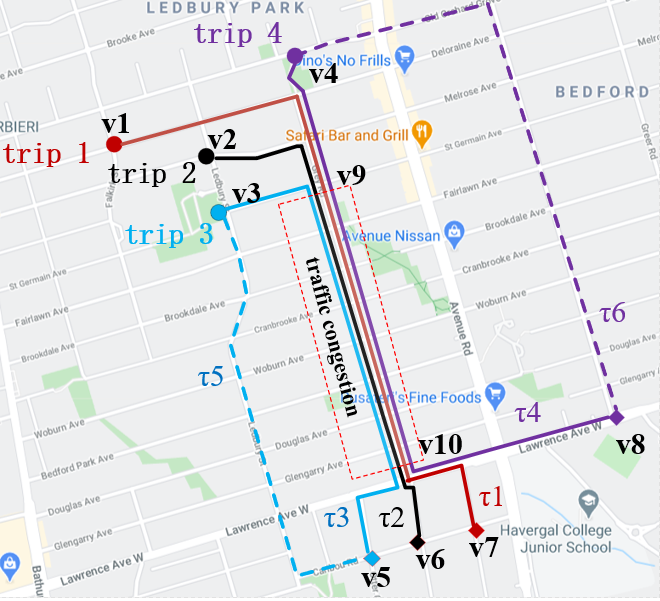
\includegraphics[width=0.6\linewidth]{fig/section3/ex1.png}
		\caption{行程请求和路线}
		\label{fig1:selfaware_ex}
    \end{figure}

以图1为例，图中的每个行程包含一个起点和终点，分别用圆圈和钻石形状标记。顶点$v_1-v_4$是行程1--4对应的起点，而顶点$v_5-v_8$是行程1--4对应的终点。行程请求1--3分别发布于8:00:01,8:00:01,8:00:05。它们的最优路线分别是$\tau_1$,$\tau_2$和$\tau_3$，在图中我们用实线标记。这三条路线预计分别会在[8:02:00,8:05:00], [8:01:40, 8:04:40],[8:01:30, 8:04:30]行驶在路段$e(v_9,v_{10})$。在[8:02:00, 8:04:30], 它们都会都会行驶在路段$e(v_9,v_{10})$，而这也许会导致交通拥堵，从而延路段$e(v_9,v_{10})$所有正在行驶的其他车辆的通行时间。行程4发布于8：00：20，基于在8：00：20这一时刻的交通状态我们为它制定的最优路线为$\tau_4$。很明显，该规划没有意识到路段$e(v_9,v_{10})$由于
之前规划的路线$\{\tau_1,\tau_2,\tau_3\}$，在未来可能会产生潜在的交通拥堵。糟糕的是，我们为行程4制定了最优路线$\tau_4$，该路线再一次经过了路段$e(v_9,v_{10})$，也许会进一步加剧交通拥堵。
综上，给定一组密集发布的行程请求流，为了缓解交通拥堵，我们需要把它们看作一个整体进行路线规划。如例1，我们可以先把行程1--3看作一个整体，考虑到可能产生的交通拥堵。我们可以调整行程3的最优路线为$\tau_5$, 在图\ref{fig1:selfaware_ex}中用虚线表示。对当前到达的行程4，通过把行程1--4看作一个整体，同理我们可以调整其最优路线为$\tau_6$。这些调整后的路线对单个请求来说也许是次优的路线，但路段$e(v_9,v_{10})$的交通拥堵却可以得到大大缓解，行程1--4总的通行时间也会大大减少。通过采用$\{tau_1,tau_2,tau_5,tau_6\}$这一路线组合，行程1--4的总的通行时间可能会是最小的，我们称这样的一个路线组合是最优的路线组合。


\subsection{研究内容与挑战}
本文提出和研究了一种针对持续的行程请求流的路线规划问题：在一个动态路网上给定一组行程请求流，行程请求流中的行程请求数是不断增加的，我们需要找到一个路线组合$\Pi=\{\pi_1,\pi_2,\ldots\}$使得所有在$\Pi$中的路线的总的通行时间最小。其中，每一条路线$\pi_i \in \Pi$是为每一个具体的行程请求$q_i$对应规划的。该问题具有十分广泛的应用场景，包括但不限于城市交通流量管理，实时的路线规划以及持续的拥堵预防上。针对该问题的精确算法具有指数级的时间复杂度，因此不能有效地运用到实际的应用场景中。为了解决这个问题，我们提出了一个自感知的批处理算法。对应的实验研究证明了该算法的准确性和高效性。
\subsection{研究成果与贡献}

\section{问题描述}

\subsection{Dijkstra 算法}
\subsection{位置点间的距离计算}
\subsection{问题定义}

\subsection{路网及其构成}
\begin{definition}[动态路网]
    一个动态路网G=(V,E)是由顶点集V和边集E构成的，其中$E\subseteq V\times V$，顶点代表路段的连接点，交叉点；连边则代表具体的路段。每条边$e(v_i,v_j)\in E$连接着两个顶点$v_i$和$v_j$，这里$v_i,v_j \in V $。为了便于描述，我们假定所有行程请求的起点和终点位置都已经被映射到离它们最近的顶点上。针对每个路段$e$, 我们用$C_e$来代表该路段的车容量，用$T_m(e)$代表在路段$e$的最小通行时间（e.g.，当路段$e$上没有其他车辆时的通行时间）。在我们的设定中，每一个路段的权重 (通行时间)是动态变化的。一个路段的最小通行时间是$T_m(e)$，而实际的通行时间是和该路段上的动态车流量成比例的。
\end{definition}

\begin{definition}[通行时间函数]
    车辆在时刻$t$经过路段$e$的通行时间和当前时刻路段$e$上的车流量$f(e,t)$相关。参照已经存在的研究\cite{Lim2012Stochastic,JavaniPath,DBLP:conf/ijcai/LiCS20}，基于当前时刻路段$e$上的车流量，我们使用下式来计算路段$e$在时刻$t$的通行时间，我们用$T(e,t)$表示。
    \begin{equation}\label{eq:tf}
    	    T(e,t)=T_m(e)\times(1+\alpha\times{(\frac{f(e,t)}{C_e})}^\beta)
    \end{equation}
    其中，$C_e$代表路段$e$的车流量，$\alpha$和$\beta$是由路段的不同性质（e.g.,限速，路宽) 等决定的可变参数。我们的解决方案是和这些参数独立的，如何为这些参数设置合适的值并不在我们的研究范围内。由式\ref{eq:tf}我们可以知道，随着车辆数目的动态变化，每条路段的通行时间也会随之发生改变。
\end{definition}

\begin{definition}[路线及其通行时间]
    我们用一个有限的顶点序列$\langle v_0,v_1,\ldots,v_{|\pi|-1}\rangle$来表示一条路线 $\pi$。假定路线$\pi$出发时间为$t_0$，$t_i$是其经过的顶点$v_i$的预计到达时间(i.e., $t_i=t_{i-1}+T(e(v_{i-1},v_i),t_{i-1})$)。结合式\ref{eq:tf}，我们用式$ET(\pi, t_0)$来计算一条路线 $\pi$的预计通行时间，即路线$\pi$中每个路段的预计通行时间之和，我们用$ET(\pi, t_0)$来表示。

    \begin{equation}\label{eq:tpi}
    ET(\pi, t_0)=\sum_{i=0}^{|\pi|-2}T(e(v_{i},v_{i+1}),t_i)
    \end{equation}
    之后我们使用$\pi.v_0$和 $\pi.v_{|\pi|-1}$ 来分别代表一条路线$\pi$对应的第一个顶点(起点)和最后一个顶点(终点)。
\end{definition}

\begin{definition}[行程请求流]
    我们用$q=(s, d, t)$来代表一个行程请求，其中$s$是该行程的起点位置，$d$是该行程的终点位置，而$t$是该行程的出发时间。$Q=\{q_1,\ q_2,\ldots\}$由多个行程请求组成，代表一组行程请求 流(i.e.,$\forall q_i,q_j\in Q, i>j$:  $q_i.t \geq q_j.t$)。需要注意的是，$Q$ 是以流数据的形式到达的行程请求集合并且$Q$是动态更新的。
\end{definition}

\begin{definition}[全局最优路径规划问题]
    在一个动态路网$G=(V,E)$上，给定一组行程请求流$Q=\{q_1,\ q_2,\ldots\}$和时间间隔$T$，持续的最优路线组合问题 (CORC问题) 旨在不断地处理最近到达的一批行程请求$Q_n=\{q_k,q_{k+1},\ldots,q_{|Q|}\}$ ($Q_n \subset Q \wedge q_{|Q|}.t-q_k.t=T$)，找到一个最优的路线组合$\Pi=\{\pi_1,\pi_2,\ldots\}$使得：
      (1) $|Q|=|\Pi|$; 
      (2) $(\forall \pi_i \in \Pi)\;(\pi_i.v_0 = q_i.s \wedge \pi_i.v_{|\pi_i|-1} = q_i.d)$; 
      (3) 在$\Pi$中规划的所有路线的总的通行时间最小，我们用$TT (\Pi)$来表示所有路线的总的通行时间 (参照公式\ref{eq:gt})。
      	\begin{equation}\label{eq:gt}
        TT (\Pi)=\sum_{i=1}^{|\Pi|}ET(\pi_i,q_i.t)
	\end{equation}
\end{definition}


\section{精确遍历算法}
针对CORC问题，一个简单直接的办法就是对每一个行程请求，搜索起点和终点间可能存在的所有路线，然后对所有的路线组合进行遍历评估，比较各个路线组合所有路线总的通行时间，最终筛选出具有最小通行时间的路线组合。具体来说，对于每一个行程请求$q_i\in Q$，我们可以采取深度优先算法(DFS)来查找从起点$s_i$到终点$d_i$可能存在的所有路线。其中，我们可以应用一些剪枝策略来加速深度优先搜索。随后，对于每一个路线组合我们计算它所有路线总的通行时间。最终，我们返回具有最小通行时间的路线组合作为返回结果。
精确算法比较简单直接，便于理解。当行程请求数量|Q|较小时，精确算法可以在有限时间内得到最优解。但是，当行程请求数量|Q|很大时，精确算法显然大量的计算时间，不能运用到实际的应用场景中。



\section{自感知的批处理算法}


为了高效解决CORC问题，我们提出了一个自感知的批处理算法 (SBP算法)，该算法主要包含两大组成部分：(1)初始路线搜索和(2)批优化处理。具体来说，给定一组行程请求流$Q_n$，我们首先采用初始路线搜索生成一个高质量的初始路线组合$\Pi_n$，该组合包含了为该行程请求流中的每个请求指定的初始路线。接下来，我们执行批优化处理对初始路线组合中的每个初始路线进行优化。最终，我们将优化后的路线组合$\Pi_n$加入到全局的路线组合$\Pi$中去。每当我们处理完一批行程请求后，我们返回$\Pi$作为实时的规划结果。我们的自感知思想合理考虑了新规划的路线会影响未来的交通状态这一事实, 即规划的路线会增加一些路段的车流量从而影响该路段的实际通行时间。
\subsection{初始路线搜索}
初始路线搜索的目标是为新一批到达的行程请求流中的每个行程请求规划一条高质量的个人路线。每个路段的动态车流量由两部分组成的，一部分是在我们规划系统中的请求车辆所造成的交通流量，即我们规划的路线在各路段上造成的车流量，我们称之为系统内的车流量，一部分是系统外的车流量即在各路段上没有使用我们规划系统的车辆数目，我们把系统外的车流量直接作为算法输入。
\subsubsection{路段标签}

为了实现对系统内车流量的快速计算，我们在每个路段上维持一系列的路段标签$L_e=\{l_1,l_2,\ldots\}$。这些路段标签记录了经过该路段的路线在该路段的时间信息。每个路段标签$l_i=\{t_a,t_b\}$记录了一条特定的路线进入路段$e$的时间$t_a$以及离开该路段的时间$t_b$。刚开始没有行程请求的时候，每个路段维持的路段标签是一个空集。之后每当我们处理完一批新的行程请求集合的时候，对应路段的路段标签会进行动态地更新。


	
	
\subsubsection{系统内的车流量计算}
 我们可以快速地计算在各个路段上由我们规划系统规划的路线所产生的车流量。由我们规划系统规划的路线在路段$e$, 时刻$t$所造成的车流量,也就是满足$[l_i.t_a, l_i.t_b] \ni t$的路段标签$l_i$的数量，其中$l_i \in L_e$。在我们的实验中，我们应用了一个优先队列来加速计算。
 

\subsubsection{通行时间下界}
我们用一个启发值$H(v_i,v_j)$来代表从一个顶点$v_i$到另一个顶点$v_j$的通行时间下界。给定最小的系统外的车流量作为静态的车流量输入，该下界是由Dijkstra 算法~\cite{Edsger1959A}预计算的。在本文中，我们将非请求车辆的车流量直接作为算法输入。


 
 
\subsubsection{算法描述}
算法~\ref{alg:alg1}提出了初始路线搜索的伪代码。算法输入包含一个动态路网$G=(V,E)$，一个行程请求$q=(v_s,v_d,t)$，所有两点间的通行时间下界$H(v_i,v_j)$，所有路段的路段标签集合$\mathcal{L}=\{L_{e_1},L_{e_2},...\}$。算法输出为行程请求$q$制定的一条初始路线。每个顶点$v\in V$ 包含以下记录信息: 从起点$v_s$到达该点的精确通行时间$t_s$；从该点到达终点的通行时间下界$t_d$；从起点到达该点的最小时刻$et$以及一个前驱节点记录$pred$。首先，我们初始化每一个顶点$v\in V$的信息记录，设置 路线 $\pi$是一个空集 (line 1)。接着我们把起点$v_s$加入一个优先队列$PQ$中。该优先队列$PQ$内部对顶点对象按照该点的$v.t_s+v.t_d$的值从小到大排序，队头元素为
具有最小$v.t_s+v.t_d$的顶点 (line 2)。在搜索过程中，每一次我们从$ PQ $选出对头元素$ v $并探索它的邻接顶点。具体来说，每一次我们选出的$ v $都具有最小的$v.t_s+v.t_d$，之所以这样选择，是基于这样的顶点扩张可能会产生最小的通行时间 (line 4)。如果选择的$v$是行程请求的终点$v_d$，我们就利用相应节点的前驱节点记录生成一条路线$\pi$，并将$\pi$作为结果返回 (lines 5--11)。如果选择的$v$不是行程请求的终点$v_d$，对于每一个从顶点$v$出发的路段$e$，我们计算当前时刻该路段的车流量 (line 13)。
对于路段$e(v, v')$的结束点$v'$，我们需要检查该点能否通过顶点$v$到达，并且所花的时间比从其他点到达该点更小 (line 14)。如果满足，我们将分别更新顶点$v'$对应的$t_s$, $et$和$pred$
记录 (lines 15--17)。接下来，如果顶点$v'$不在优先队列$PQ$中，我们将其加入。当优先队列$PQ$为空或者我们已经扩张到行程请求对应的终点时，初始路线搜索算法终止。


初始路线搜索： 对于每一个新到达的行程请求（包含起点，终点，出发时刻），寻找一条在出发时刻出发，从起点能最快到达终点的路径（最短路径）。假设车辆通过特定路段的时间是和该路段的属性和车流量决定的，而车流量由两部分组成。一部分是非请求车辆车流量，即没有使用我们路线规划系统的车辆，直接作为输入数据，不是我们研究的范畴；一部分是请求车辆的车流量，即使用了我们规划系统的车辆，这些车辆按照规划的路线行驶而在经过的路段上增加的车流量。由于路网每个路段车流量是动态变化的，通行时间也会随之动态变化，我们就是要在这样一个动态变化的路网中寻找从出发时刻出发，起点到终点的最短路径。

初始路线搜索过程从起点开始，对与起点相连的邻接顶点做网络扩张，接着选择一个新的顶点继续扩张，直到扩张到终点。我们的扩张策略是，每次选择一个最可能最快到达终点的顶点作为下一个扩张顶点，什么是最可能最快到达终点的顶点呢？即 （从起点到该点的精确耗时+从该点到终点的最小耗时） 最小的顶点。从起点到该点的精确耗时是根据每个路段的实时车流量准确计算出来的，而从该点到终点的最小耗时是预处理中计算的。在预处理中，我们取每个路段的最小车流量作为静态的车流量，利用dijkstra算法计算顶点两两之间的最短路径（即耗时最小的路径），并将顶点两两之间的最小耗时存储起来作为我们初始路线搜索的算法输入。综上，我们从起点开始，按照该扩张策略一直扩张，直到扩张到终点，则我们就找到了一条在出发时刻能最快到达终点的路径。

批优化处理：
对于在较短时间间隔(比如1s)内发出的行程请求集合（包含起点，终点，出发时刻），我们为这些请求分别调用初始路线搜索后，这些初始路线可能会导致潜在的拥堵，从而增加对应路段的通行时间， （比如说行程数量很多，而为它们规划的路线都要经过同一路段，则可能造成拥堵)。因此这些最优路线的部分路段是需要优化的，我们将在同一时间间隔(比如1s)内发出的行程请求作为一个整体，对我们之前为它们规划的初始路线集合进行批优化处理。
对于一批初始路线集合，我们批优化策略如下：
1）从该集合中选取其中一条路线，将该集合内的其他路线看作已经发布的路线 (其实还没有发布)，假定这些用户将会按照发布的路线行驶，对应道路上就会增加一定车流量，从而全局车辆（包括之前已经规划的车辆在每个路段的耗时也会变化）。我们需要计算这些路线在各个路段增加的车流量，更新路段上的车流量，更新所有行程在各路段的通行时间，这些就相当于更新了交通信息。
2) 对于这个选取的初始路线，我们根据1）更新的交通信息，重新查找一条从起点到终点的最短路径。如果该最短路径不是原来的初始路线且经过计算该最短路径可以减少全局所有行程的耗时超过一定幅度，我们称新搜索到的这条最短路线是有效的，将原来的初始路线更新为新的最短路径。
3）重复1）2）过程直到对于每一条路线，都不存在新的有效最短路径。将该批次优化后的路线发布给用户。

\begin{algorithm}[!h]
    \caption{InitSearch($G,q,\mathcal{L}$)}
    \label{alg:alg1}
    
    \Input{
    动态路网 $G=(V,E)$；\newline
    行程请求 $q=(v_s,v_d,t)$；\newline
    所有两点间的通行时间下界 $H(v_i,v_j)$；\newline
    规划路线的路段标签集合 $\mathcal{L}$。
    }
    \Output{
    为请求 $q$ 制定的初始化路线 $\pi$。
    }
    
    \textbf{Init:}
    $\forall v\in V$: $v.t_s=\infty$, $v.t_d=H(v,v_d)$, $v.et=t$；\newline
    $v_s.pred=null$, $v_s.t_s=0$；$\pi=\emptyset$；
    
    $PQ \leftarrow \{v_s\}$；
    
    \While(\tcc*[f]{主搜索循环}){$PQ \neq \emptyset$}{
        $v \leftarrow PQ.pop()$；
    
        \If(\tcc*[f]{到达目的节点}){$v = v_d$}{
            \While{$v_d.pred \neq null$}{
                $\pi \leftarrow \{v_d, \pi\}$；
                $v_d \leftarrow v_d.pred$；
            }
            \textbf{return} $\pi$；
        }
    
        \For(\tcc*[f]{遍历邻接路段}){each edge $e(v,v') \in G$}{
            计算当前时刻 $v.et$ 下路段 $e$ 的通行时间 $T(e,v.et)$；
    
            \If{$v.t_s + T(e,v.et) \leq v'.t_s$}{
                $v'.t_s \leftarrow v.t_s + T(e,v.et)$；
                $v'.et \leftarrow t + v'.t_s$；
                $v'.pred \leftarrow v$；
    
                \If{$v' \notin PQ$}{
                    $PQ.push(v')$；
                }
            }
        }
    }
    \end{algorithm}
	







    
    
    

    \subsection{批优化处理}
    为了提高算法质量，我们提出了一个批优化处理方法对由算法\ref{alg:alg1}产生的初始路线进行优化。一个初始路线组合$\Pi_n$包含了为最近到达的行程请求$Q_n$制定的初始路线。不同于$\Pi_n$的是，全局的路线组合$\Pi$包含了所有在当前时间之前已经规划的路线。优化处理过程重新利用了初始路线组合$\Pi_n$，并通过一种自感应的批处理交换策略对$\Pi_n$中的每一条初始路线进行优化。批优化处理的精髓在于：在每一个优化过程中，我们选择一条路线$\pi_i \in \Pi_n$。我们将除了该路线的其他正在规划的初始路线作为已知的路线规划输入到交通流量信息中，重新预测未来的交通状态并尝试重新分配一条新的路线$\pi_i'$给行程$q_i$。我们用$\pi'$对原始地初始路线$\pi \in \Pi_n$进行交换，该交换操作可以用$\Pi_n.swap(\pi,\pi')$
   表示。如果该交换操作能够使所有行程的通行时间之和减少至少1 + $\epsilon$的比例 (e.g., $\frac{TT(\{\Pi, \Pi_n\})}{TT(\{\Pi, \Pi_n.swap(\pi,\pi')\})}>(1+\epsilon)$)，我们认为该操作是有效的并采用该操作去更新原有的初始路线。其中，我们采用一个极小的常数值$\epsilon$排除一些"无用"的操作，这里无效操作指通过该操作只能减少很小的通行时间。此外，$\epsilon$的使用还保证了交换操作的次数是有限的。实际上，有效的交换操作的次数是和$\epsilon$成反比的。具体来说，最大的有效交换操作的次数是$log_{(1+\epsilon)} \frac{TT}{TT_{m}}$。其中$TT$是当前规划的初始路线组合的总的通行时间，而$TT_{m}$是理想的最小通行时间。当路线组合$Q_n$中不存在有效交换操作，不能
  再产生一个更好的规划结果，批优化处理算法终止。在本文中，我们也提出了一个预检查策略来进一步提高效率。
	  
	\subsubsection{交换操作}
	在优化过程中，除了考虑系统外车流量和系统内已经规划的路线产生的车流量外，我们进一步考虑了当前正在规划的初始路线可能对未来交通产生的潜在影响。一个新的路段标签集合$\mathcal{L}'=\{\mathcal{L},\mathcal{L}(\Pi_n\setminus \pi_i)\}$ 是由原有的路段标签$\mathcal{L}$以及预估的正在规划的初始路线的时间信息联合组成的 (cf. 算法 \ref{alg:alg1})。把$\mathcal{L}'$作为已知的交通信息输入，我们再次执行算法\ref{alg:alg1}为行程$q_i$分配一条新的路线$\pi_i'$。如果该交换操作被确定是有效的，我们将使用新路线$\pi_i'$替换原有的路线$\pi_i\in \Pi_n$ 。
	
	\subsubsection{预检查策略} 
	为了检查一个交换操作的有效性，我们必须更新所有路段的路段标签去计算所有行程总的通行时间的降低率，这是非常费时的。因此，我们提出了一个预检查策略进一步提高算法效率。具体来说，我们定义了一个所有行程总的通行时间的降低率上界$UB$，计算如下。 
	\begin{equation}\label{eq:pre-check}
	   % UB(\pi) = TT(\{\Pi,\Pi'\}) - TT(\{\Pi,\Pi' \setminus \pi\})
	   UB(\pi) = \frac{TT(\{\Pi,\Pi_n\})}{TT(\{\Pi,\Pi_n \setminus \pi\}}
	\end{equation}
	 注意$TT(\{\Pi,\Pi_n \setminus \pi\}) \neq TT(\{\Pi,\Pi_n\})-ET(\pi,t)$, 在这里 $TT(\{\Pi,\Pi_n \setminus \pi\})$ 是将路线$\pi$剔除，假设该路线不存在下的所有路线的总的通行时间。我们不仅要剔除路线$\pi$本身的通行时间，也要消除路线$\pi$对其他行程的影响，因为路线$\pi$造成了额外的交通流量，会对其他路线的通行时间造成一定的影响。
	
     \begin{algorithm}[!h]
        \caption{BatchRefining($G,\Pi,\Pi_n,\mathcal{L},\epsilon$)}
        \label{alg:alg2}
        
        \Input{
        动态路网 $G=(V,E)$；\newline
        全局路线组合 $\Pi$；\newline
        初始路线组合 $\Pi_n$；\newline
        路段标签集合 $\mathcal{L}$；\newline
        参数 $\epsilon$。
        }
        \Output{
        优化后的路线组合 $\Pi_n$。
        }
        
        \textbf{Init:} $flag \leftarrow true$；
        
        \While(\tcc*[f]{批量迭代优化}){$flag$}{
            $flag \leftarrow false$；
        
            \For(\tcc*[f]{遍历当前路线集合}){each route $\pi_i \in \Pi_n$}{
                \If{$UB(\pi_i) > (1+\epsilon)$}{
                    $\mathcal{L}' \leftarrow \{\mathcal{L}, \mathcal{L}(\Pi_n \setminus \pi_i)\}$；
        
                    $\pi' \leftarrow InitSearch(G,q_i,\mathcal{L}')$；
        
                    \If(\tcc*[f]{可行替换}){操作 $\Pi_n.swap(\pi_i,\pi')$ 是有效的}{
                        $\Pi_n \leftarrow \Pi_n.swap(\pi_i,\pi')$；
                        $flag \leftarrow true$；
                    }
                }
            }
        }
        \end{algorithm}
	
	\subsubsection{算法描述}
	算法\ref{alg:alg2}提出了批优化处理算法的伪代码。初始地，我们使用一个标志flag来标记在上一次"while"循环中是否存在有效的操作，算法开始我们设置其为true (line 1)。在优化过程中，对于每一条初始路线$\pi \in \Pi_n$，我们检查它能否被一条新的路线$\pi'$替换 (lines 4--13)。具体来说，我们首先更改标志flag为false,假设在本轮循环中不存在有效的交换操作 (line 3)。对于每一条路线$\pi \in \Pi_n$，我们通过计算提升上界$UB(\pi)$来预检查该交换操作的有效性。如果该交换操作是可能有效的，我们生成一个新的路段标签 $\mathcal{L}'$(line 6). 将$\mathcal{L}'$作为输入，我们执行算法 \ref{alg:alg1}产生一条新的路线$\pi'$(line 7). 如果该交换操作最终被
    确定是有效的，我们将采用这次交换操作并设置标志flag为true来记录当前循环仍然具有有效的交换操作 (lines 8--11). 当一轮循环，对所有的$\pi \in \Pi_n$都没有检测到有效的交换操作，算法终止。也就是说已经没有能够产生更好结果的有效操作存在。
	
	\subsection{CORC问题的总体解决方案}
	通过整合上文提出的所有方法，我们在这里提出针对CORC问题的总体解决方案即SBP算法。SBP算法执行流程如下：对于每一个新到达的行程请求$q$，我们先执行初始路线搜索为其分配一条初始个人路线。接着我们执行算法\ref{alg:alg1}周期性的批优化最近规划的初始路线，这些初始路线是为最近一段时间发布的行程请求制定的。一旦有新的行程请求发布，SBP算法将不断执行上述操作。
	
	\subsubsection{优化间隔}
	在我们的设定中，批优化算法是以固定的时间间隔周期性执行的 (e.g., 2s)。我们用$T$表示每两次批优化处理之间的时间间隔。通过利用这样一个时间间隔$T$，我们合理考虑了更多的正在规划的初始路线对未来交通的潜在影响，在这种情况下我们能更准确地预测未来的交通状态，从而通过一次交换操作我们也许可以减少更多的通行时间，整个优化过程中总的交换次数也会减少，算法效率也就得到了提高。
    \begin{algorithm}[!h]
        \caption{SBP($G,Q,T,\epsilon$)}
        \label{alg:alg3}
        
        \Input{
        动态路网 $G=(V,E)$；\newline
        行程请求流 $Q$；\newline
        优化时间间隔 $T$；\newline
        参数 $\epsilon$。
        }
        \Output{
        实时的最优路线组合 $\Pi$。
        }
        
        \textbf{Init:}
        $\mathcal{L} \leftarrow \emptyset$；
        $\Pi \leftarrow \emptyset$；
        $\Pi_n \leftarrow \emptyset$；
        
        \While(\tcc*[f]{系统持续运行}){\textbf{true}}{
        
            \For(\tcc*[f]{处理到达的行程请求}){each trip request $q \in Q$}{
                $\pi \leftarrow InitSearch(G,q,\mathcal{L})$；
                $\Pi_n \leftarrow \{\Pi_n,\pi\}$；
            }
        
            \If(\tcc*[f]{周期性批量优化}){当前时间 $\bmod\, T = 0$}{
                $\Pi_n \leftarrow BatchRefining(G,\Pi,\Pi_n,\mathcal{L},\epsilon)$；
                $\Pi \leftarrow \{\Pi,\Pi_n\}$；
                $\mathcal{L} \leftarrow \{\mathcal{L},\mathcal{L}(\Pi_n)\}$；
                $\Pi_n \leftarrow \emptyset$；
        
                \textbf{Output} $\Pi$ \tcp*[f]{实时输出结果}
            }
        }
        \end{algorithm}
	\subsubsection{算法描述}
	算法 \ref{alg:alg3}提出了针对CORC problem的总体解决方案，即SBP算法的伪代码。
	初始地，我们的规划系统中没有接收到任何行程请求，我们设置路段标签$\mathcal{L}$和全局的路线组合$\Pi$都是空集。全局的路线组合$\Pi$记录了所有已经规划完毕的行程的路线。我们也使用了一个路线组合$\Pi_n$来记录为新的一批行程$Q_n$规划的初始路线，初始的$\Pi_n$也是空集 (line 1). 首先我们执行算法\ref{alg:alg1}为每一个新到达的行程$q \in Q$请求分配一条初始化路线 (lines 3--6)。我们持续地为新到达的请求生成初始路线直到下一次批优化处理 (line 7)。在批优化处理过程中，我们执行算法\ref{alg:alg2}去生成一个优化后的路线组合$\Pi_n$ (line 8)。接下来，我们将这些优化后的路线加入全局的路线组合$\Pi$中，并根据新规划的路线对所有路段的路段标签记录进行更新 (lines 9--10)。
	   每一个优化处理完成后，由于所有的初始路线已经被优化了，我们设置$\Pi_n$为空并继续用于记录下一批到达的行程的初始路线 (line 11)。每当我们处理完一批新的行程请求流，我们输出全局最优的路线组合$\Pi$作为实时的规划结果 (line 12)。
    
   

\section{实验研究}
	
\subsection{实验设定}
\subsubsection{数据集}
我们使用两个路网数据集用于我们的实验研究：
 San Joaquin County Road Network  (TG路网)\footnote{https://www.cs.utah.edu/~lifeifei/SpatialDataset.htm}和 the New York Road Network  (NY路网)\footnote{https://publish.illinois.edu/dbwork/open-data}.
 我们用邻接表进行路网图的存储。对于每个路段连边，我们基于该路段的长度分配一个数值为20--100间的车容量$C_e$。每个路段的最小通行时间$T_m(e)$是随机生成的，位于5--10分钟之间。为了模拟非请求车辆，我们假设每个路段$e$上的非请求车辆的平均车流量$\bar{x}$为0.4$\times C_e$，实时的非请求车辆在平均车流量附近周期性地动态变化0.8$\bar{x}$ 到1.2$\bar{x}$。
给定最小的非请求车流量0.8$\bar{x}$作为所有路段的静态车流量，我们提前计算好所有顶点两两间的通行时间下界,该下界即算法\ref{alg:alg1}中的启发值$H(v_i,v_j)$。在路网较为密集的区域，我们随机采样起点-终点对来模拟行程请求。为了模拟持续到达的行程请求流，给定第一个行程的出发时间$q_1.t$，接下来的第i个行程的出发时间$q_i.t$在上一个行程请求的出发时间$q_{i-1}.t$的基础上小幅度增加或保持不变。行程请求到达的速率设定见表\ref{tb:para}。


\subsubsection{车流量的计算}
在我们的实验设定中，在时刻$t$路段$e$ 实时的车流量$f(e,t)$是由式~\ref{eq:flow}计算的。
\begin{equation}\label{eq:flow}
f(e,t) = f{'}(e,t)+f{''}(e,t)
\end{equation}
其中，$f{'}(e,t)$代表系统外的非请求车辆的车流量，而$f{''}(e, t) $代表系统内请求车辆的车流量。为了模拟非请求车辆，我们假设$f{'}(e,t)$是随时间周期性动态变化的 (e.g.,$f{'}(e,t+T)$=$f{'}(e,t)$ ,T=2h)。如何计算系统内请求车辆的车流量我们已经在算法\ref{alg:alg1}中给出。

\begin{table}
\centering
\begin{tabular}{|p{3.2cm}|p{4cm}|p{4cm}|}
    \hline
    \bfseries & \bfseries TG路网 & \bfseries NY 路网\\
    \hline
    行程请求数 \textbf{$|Q|$} & \tabincell{c}{4,000-20,000 | default 4,000} &  \tabincell{c}{2,000-10,000 | default 2,000} \\
    \hline
    参数 $ \epsilon $ &
    \tabincell{c}{0.0002-0.0010 | default 0.001}& \tabincell{c}{0.0002-0.0010 | default 0.001} \\
    \hline
    优化间隔 \textbf{T} &
    \tabincell{c}{1s-5s | default 2s}& \tabincell{c}{1s-5s | default 2s} \\
    \hline
    行程到达速率 &
    \tabincell{c}{20/s-100/s | default 50/s}& \tabincell{c}{20/s-100/s | default 50/s} \\
    \hline
    $ \alpha$ (cf. 式 \ref{eq:tf}) & \tabincell{c}{1-5 | default 2}& \tabincell{c}{1-5 | default 2} \\
    \hline
    $\beta$ (cf. 式 \ref{eq:tf}) & \tabincell{c}{1-3 | default 2}& \tabincell{c}{1-3 | default 2} \\
    \hline
\end{tabular}
\caption{参数设定}
\label{tb:para}
\end{table}


\subsubsection{算法评估设定}
我们主要评估了自感应批处理算法 （SBP算法) 的算法表现。为了评估该算法的结果质量，我们额外实施了一个基于个人的搜索算法 (Ind 算法)。具体来说，给定一组行程请求流$Q$，对于每一个行程请求$q \in Q$， Ind算法基于单个行程的出发时刻的交通状态生成一条最优的个人最优路线，这和一些已经存在的研究相符 \cite{DBLP:conf/icde/MalviyaMB11,DBLP:conf/dasfaa/XuGDSL12}. 由于精确算法十分耗时，在默认设定下需要至少一天的时间，因此我们不研究精确算法的表现。我们知道SBP算法由两部分组成：初始路线搜索和批优化处理。我们提出的的初始路线搜索合理考虑了自感应的思想和网络的动态性，为了验证其优越性，我们分别又实施了SBP*SA算法和SBP*DA算法。 其中，SBP*SA算法是初始路线搜索没有采用自感知思想的SBP算法，即它没有考虑由我们规划系统规划的路线随交通流量造成的额外影响。SBP*DA
算法是没有考虑网络动态性的SBP算法，它在初始路线搜索过程中面向的是一个静态的交通状态快照即一个行程的出发时刻所对应的静态交通状态。
我们使用CPU运行时间和所有行程总的通行时间$TT(\Pi)$作为算法效率和算法准确性的评估指标。除非特别申明，我们的实验结果是超过20次独立实验的平均值结果。所有的算法都是在windows10平台上运行的，采用Java编程，使用Intel(R) Core(TM) i5-9300H Processor (2.40 GHz)的处理器和16GB的内存。具体的默认参数设定见表\ref{tb:para}。

\subsection{实验结果}
\subsubsection{行程请求数目对算法效果的影响}

\begin{figure*}[h]
% 	Figure 1 effect Of Query Count
    \centering
        \subfloat[NY]{
            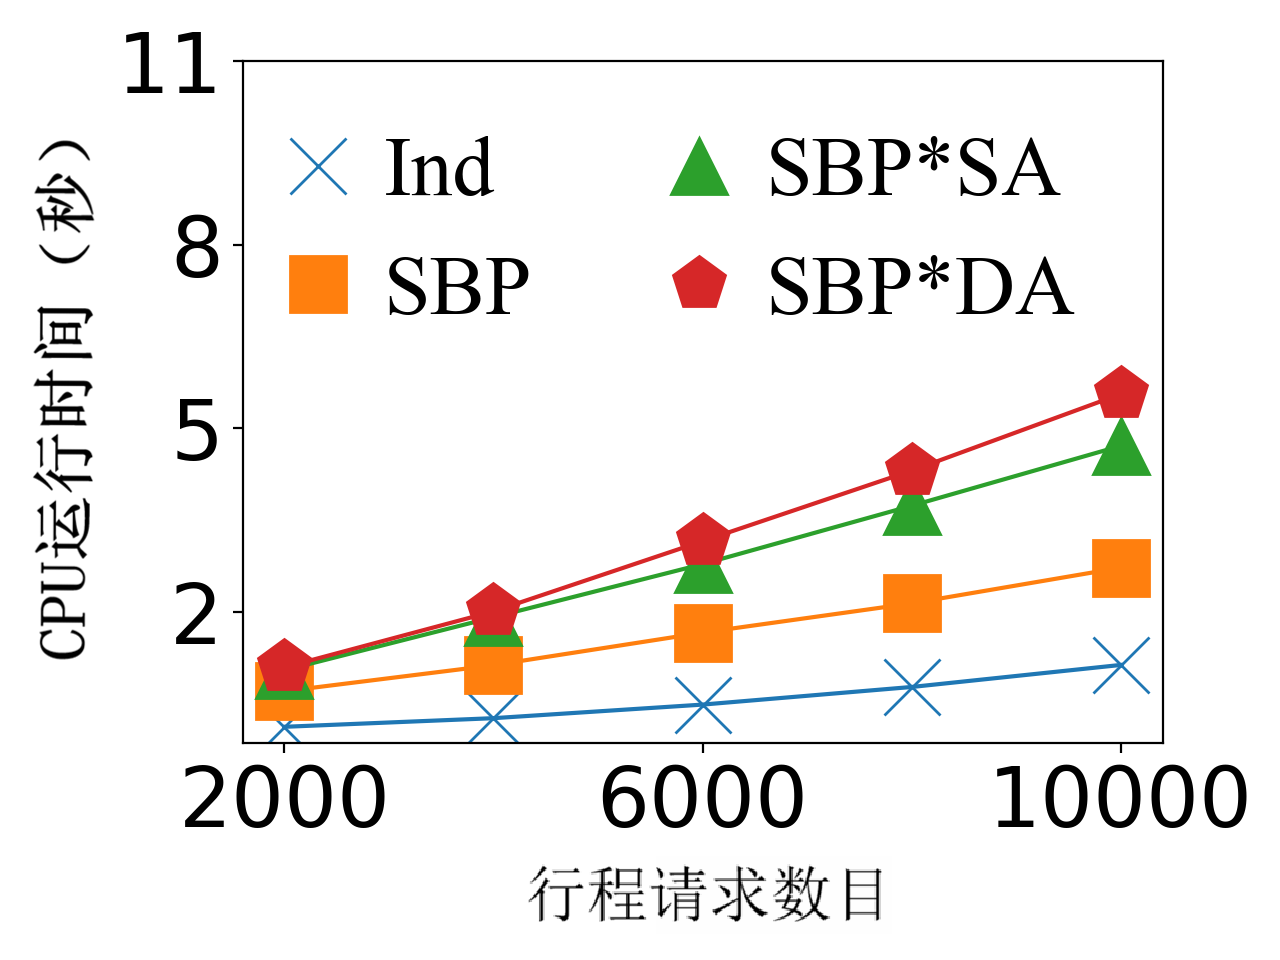
\includegraphics[width=0.4\linewidth]{fig/section3/fig1_NYC_time.png}
            \label{fig1:a}
        }%
        \hfill
        \subfloat[NY]{
        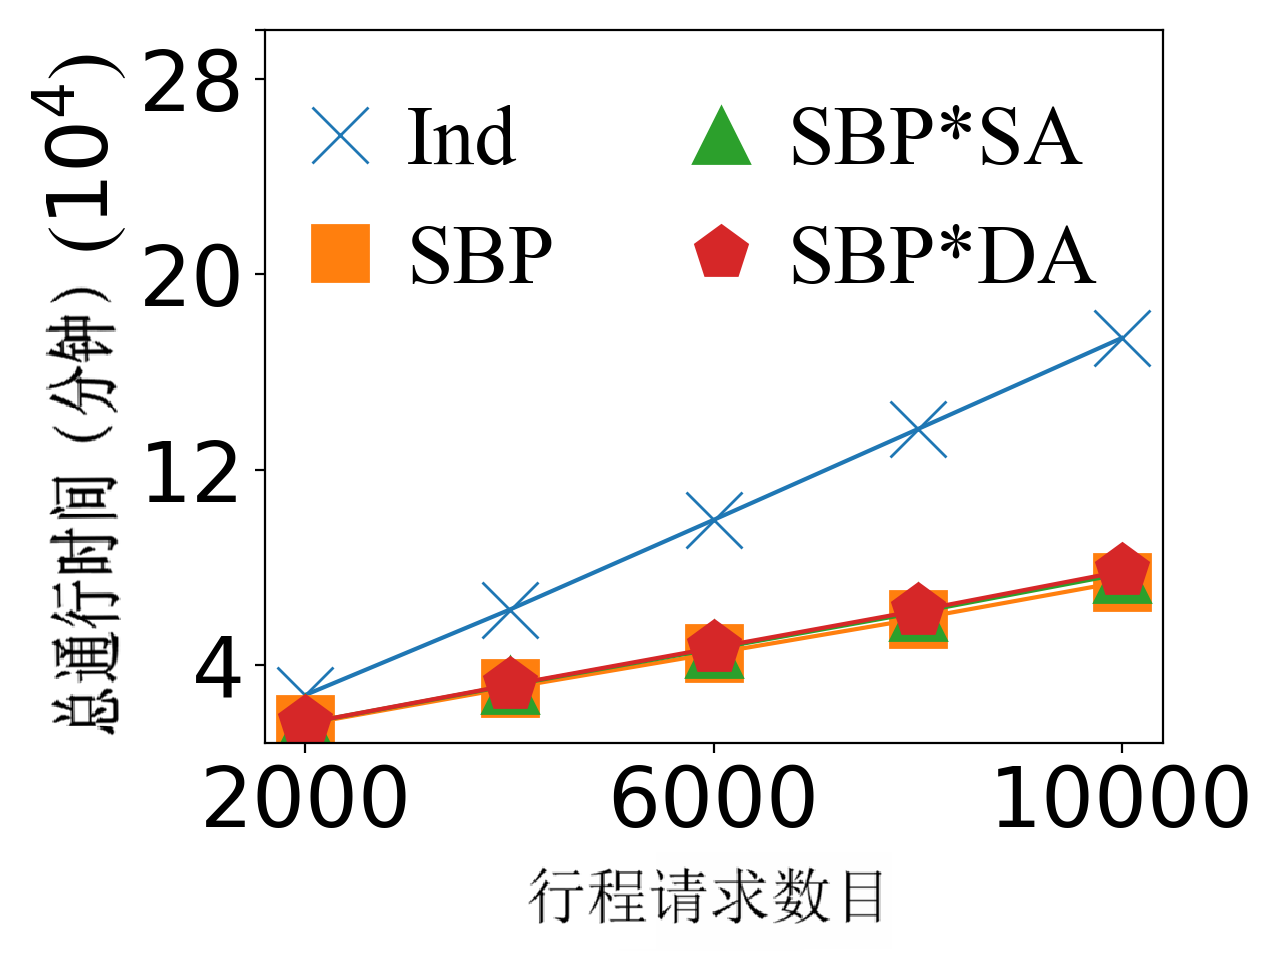
\includegraphics[width=0.4\linewidth]{fig/section3/fig1_NYC_cost.png}
            \label{fig1:b}
        }%
        \\
        \subfloat[TG]{
        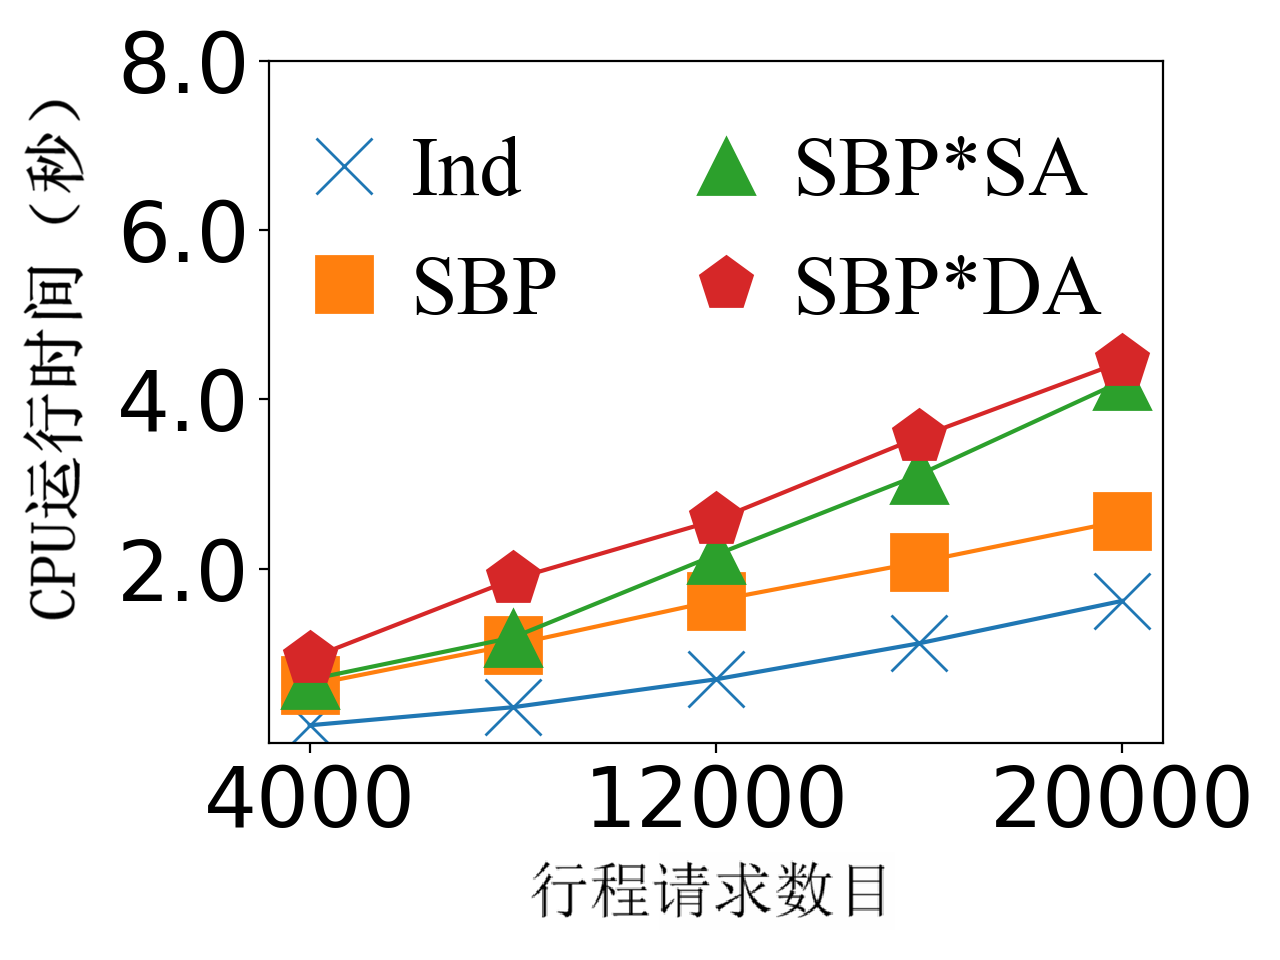
\includegraphics[width=0.4\linewidth]{fig/section3/fig1_TGC_time.png}
            \label{fig1:c}
        }%
        \hfill
        \subfloat[TG]{
        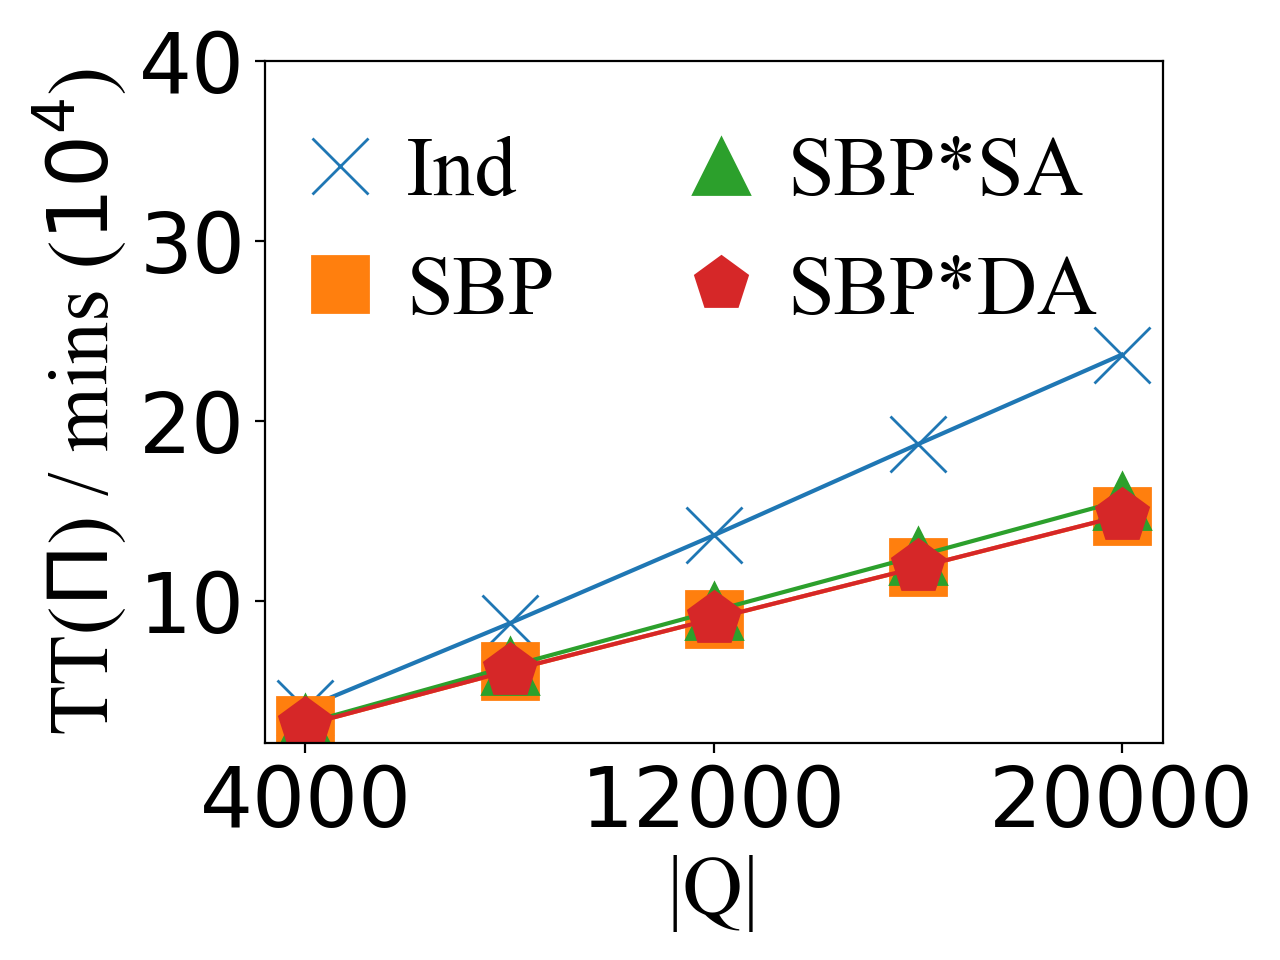
\includegraphics[width=0.4\linewidth]{fig/section3/fig1_TGC_cost.png}
            \label{fig1:d}
        }%
        \caption{行程请求数目$|Q|$的影响}
        \label{fig1}
    \end{figure*}


\begin{figure*}[h]
% Figure 2 effect Of Query arrival rate
\centering
        \subfloat[CPU time]{
            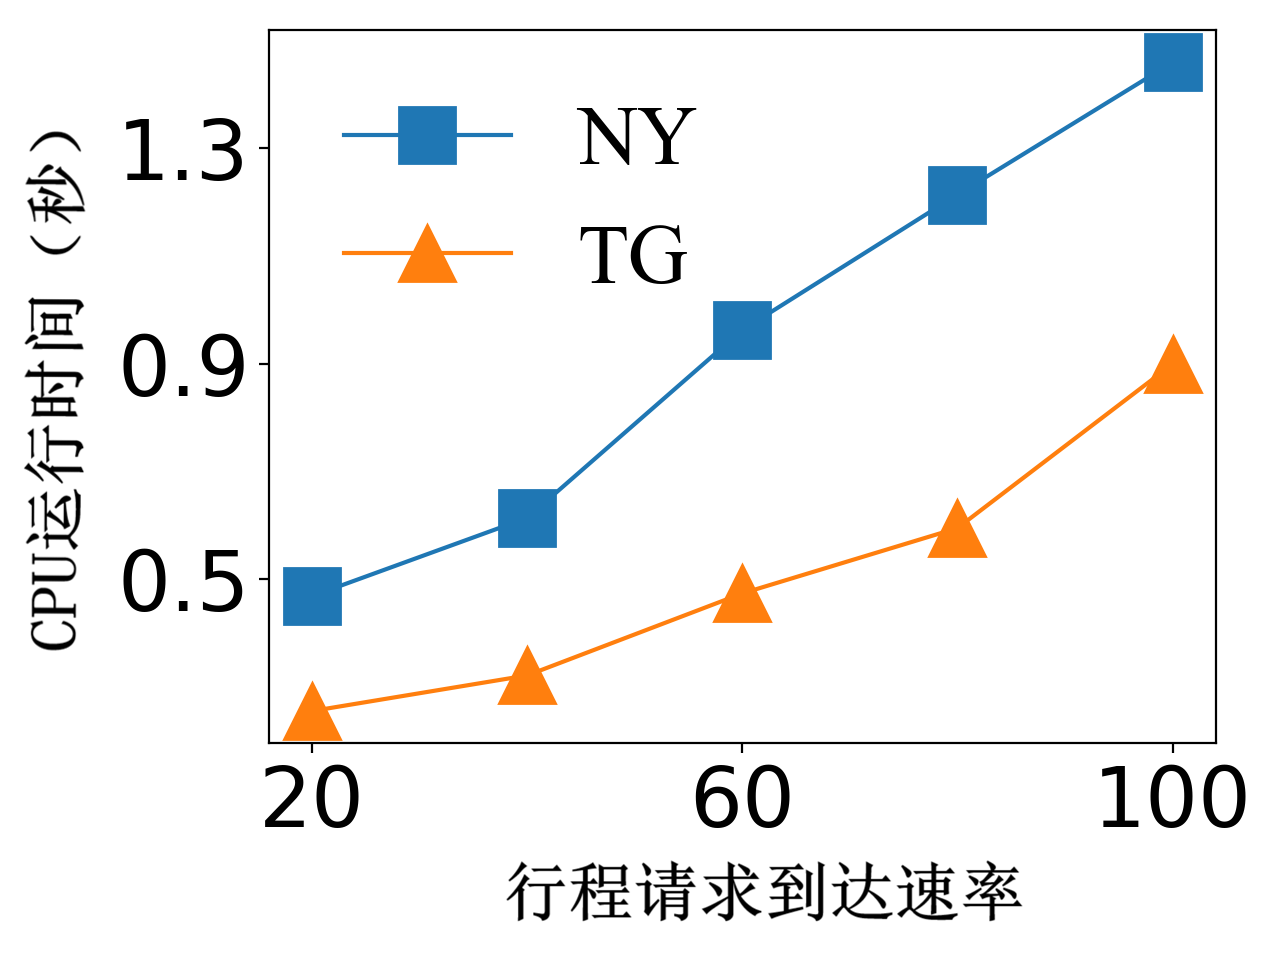
\includegraphics[width=0.4\linewidth]{fig/section3/fig2_time.png}
            \label{fig2:a}
        }% 
        \hfill
        \subfloat[Travel time]{
        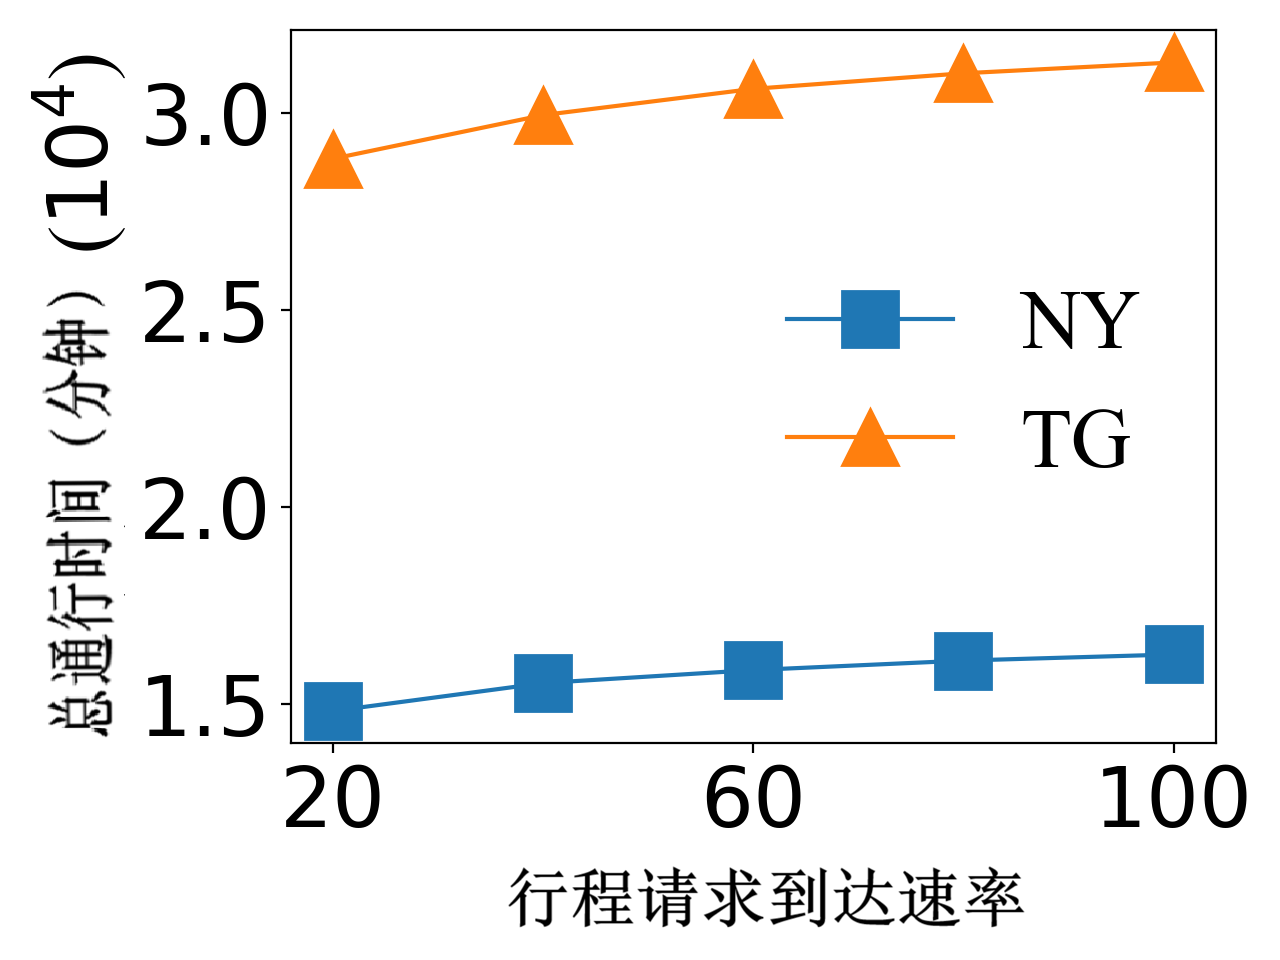
\includegraphics[width=0.4\linewidth]{fig/section3/fig2_cost.png}
            \label{fig2:b}
        }%
        \caption{行程请求到达速率的影响}
        \label{fig2}
\end{figure*}

\begin{figure*}[htbp]
% Figure 3 effect Of Refining Interval
\centering
        \subfloat[CPU time]{
            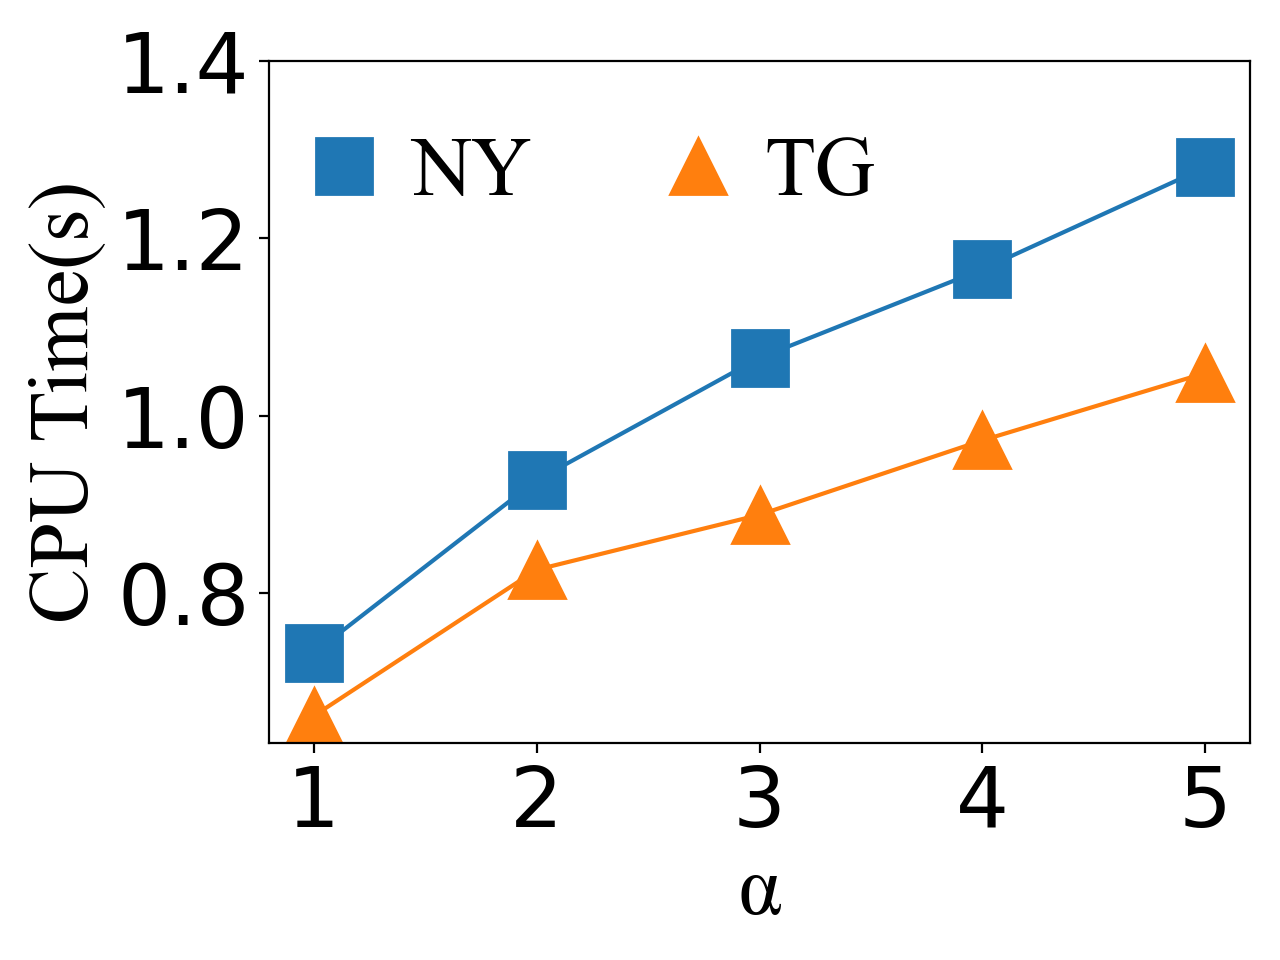
\includegraphics[width=0.4\linewidth]{fig/section3/fig3_alpha_time.png}
            \label{fig3:a}
        }%
        \hfill
        \subfloat[Travel time]{
        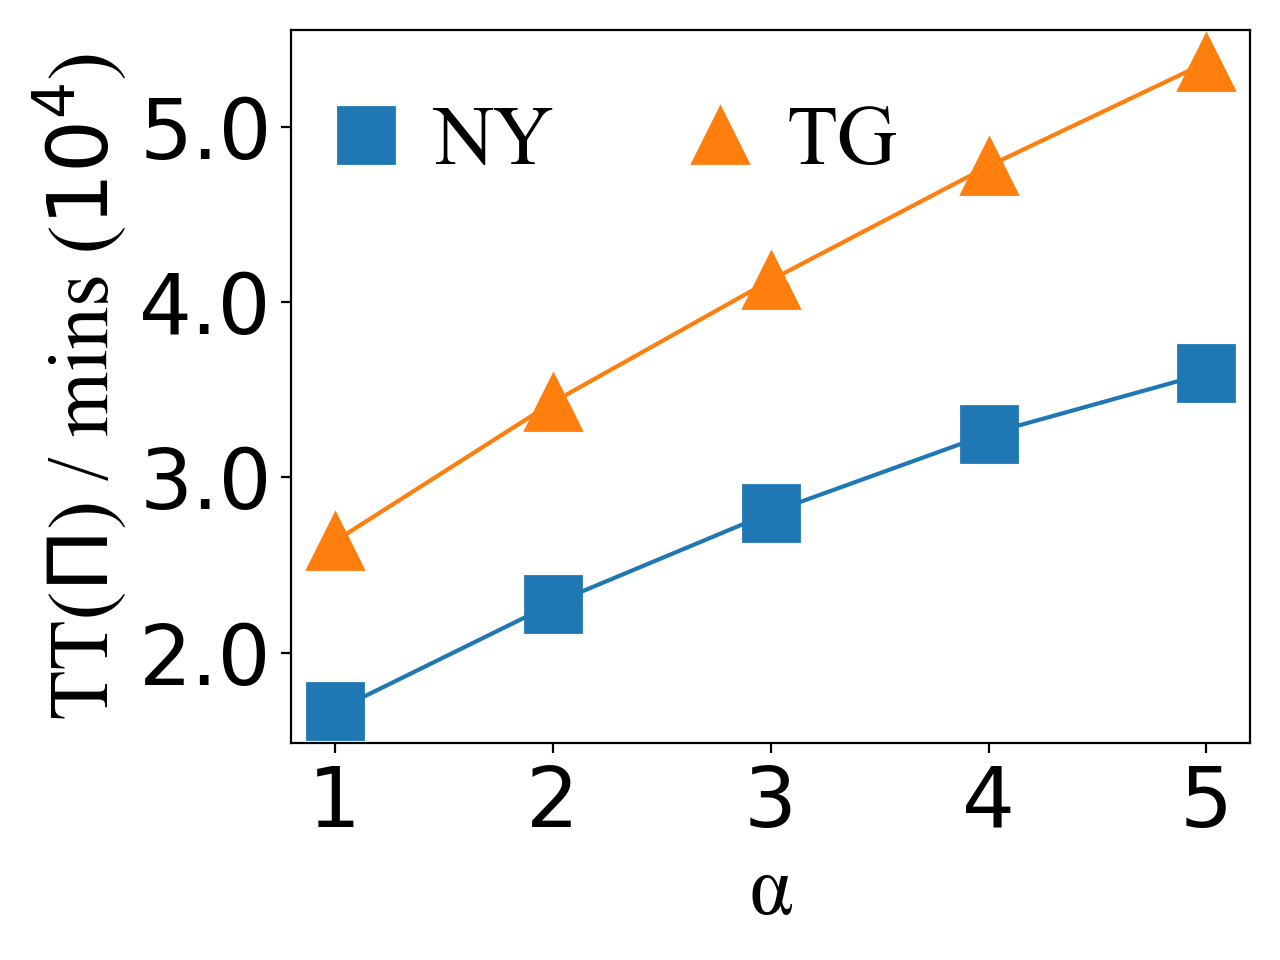
\includegraphics[width=0.4\linewidth]{fig/section3/fig3_alpha_cost.png}
            \label{fig3:b}
        }%
        \\
        \subfloat[CPU time]{
        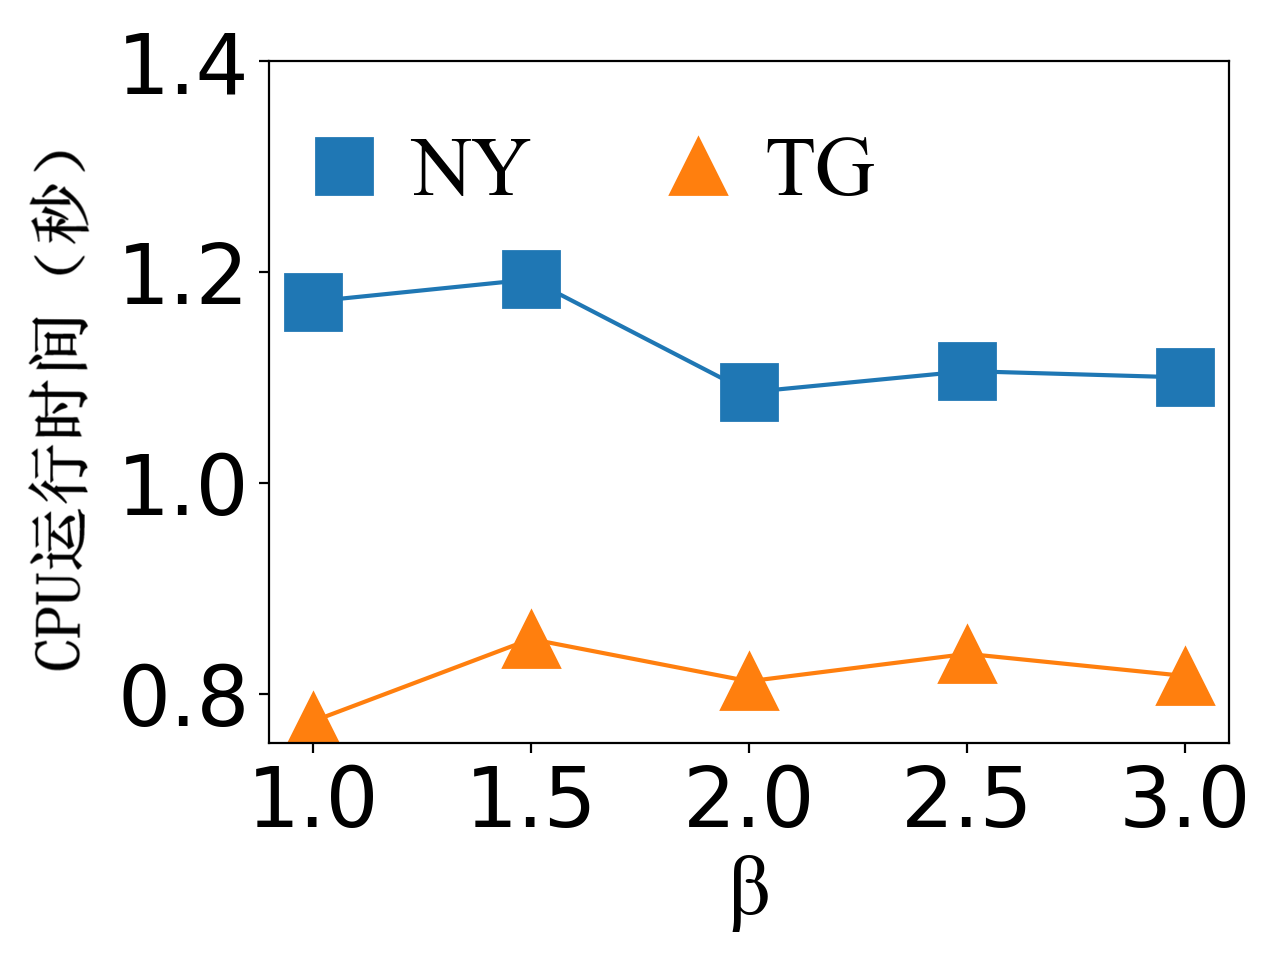
\includegraphics[width=0.4\linewidth]{fig/section3/fig3_beta_time.png}
            \label{fig3:c}
        }%
        \hfill
        \subfloat[Travel time]{
        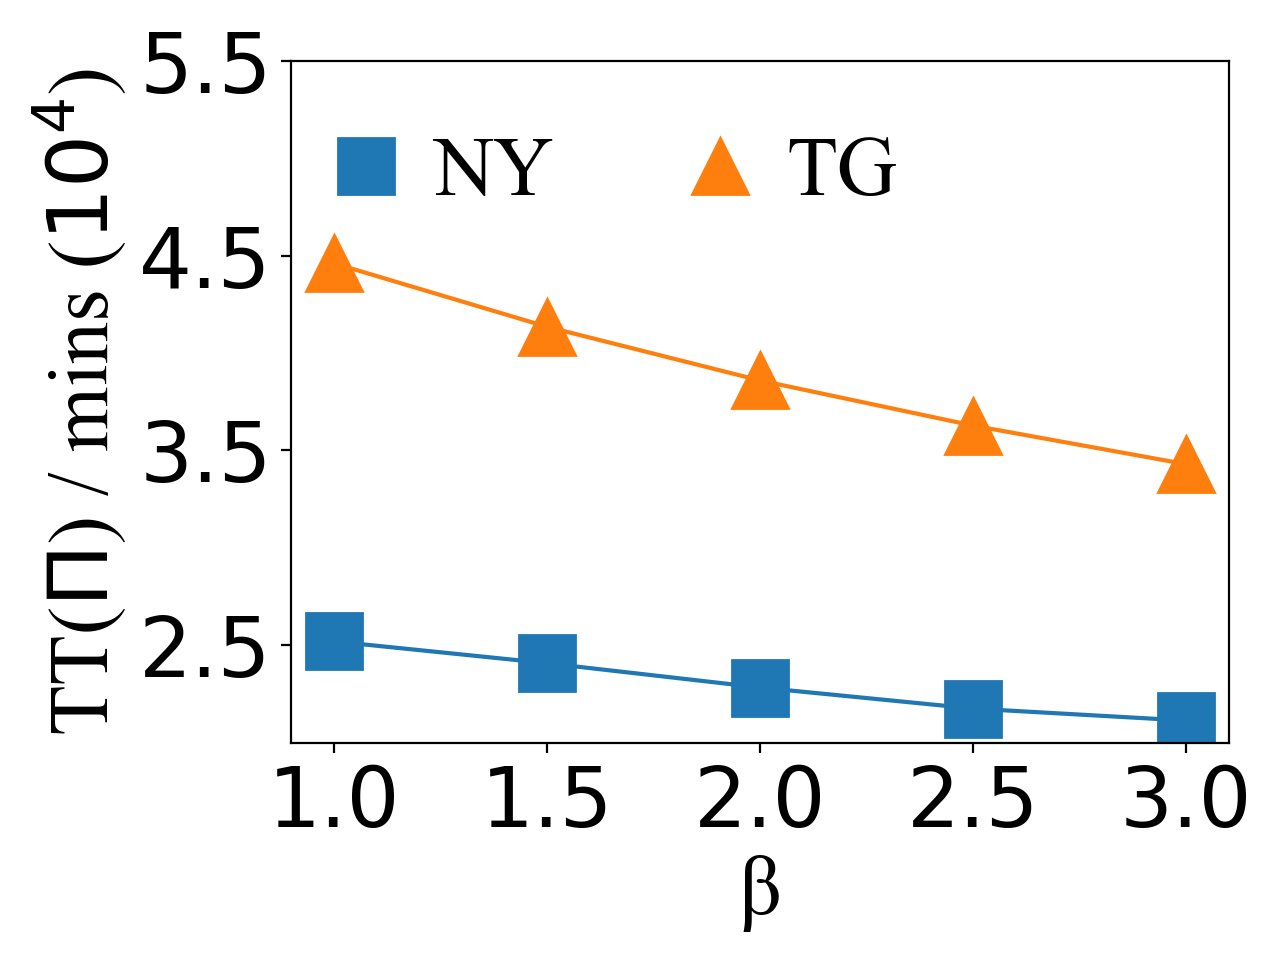
\includegraphics[width=0.4\linewidth]{fig/section3/fig3_beta_cost.png}
            \label{fig3:d}
        }%
        \caption{参数 $\alpha$ \& $\beta$的影响}
        \label{fig3}
    \end{figure*}
% Figure 4 effect Of T
\begin{figure*}[htbp]
    \centering
        \subfloat[CPU time]{
            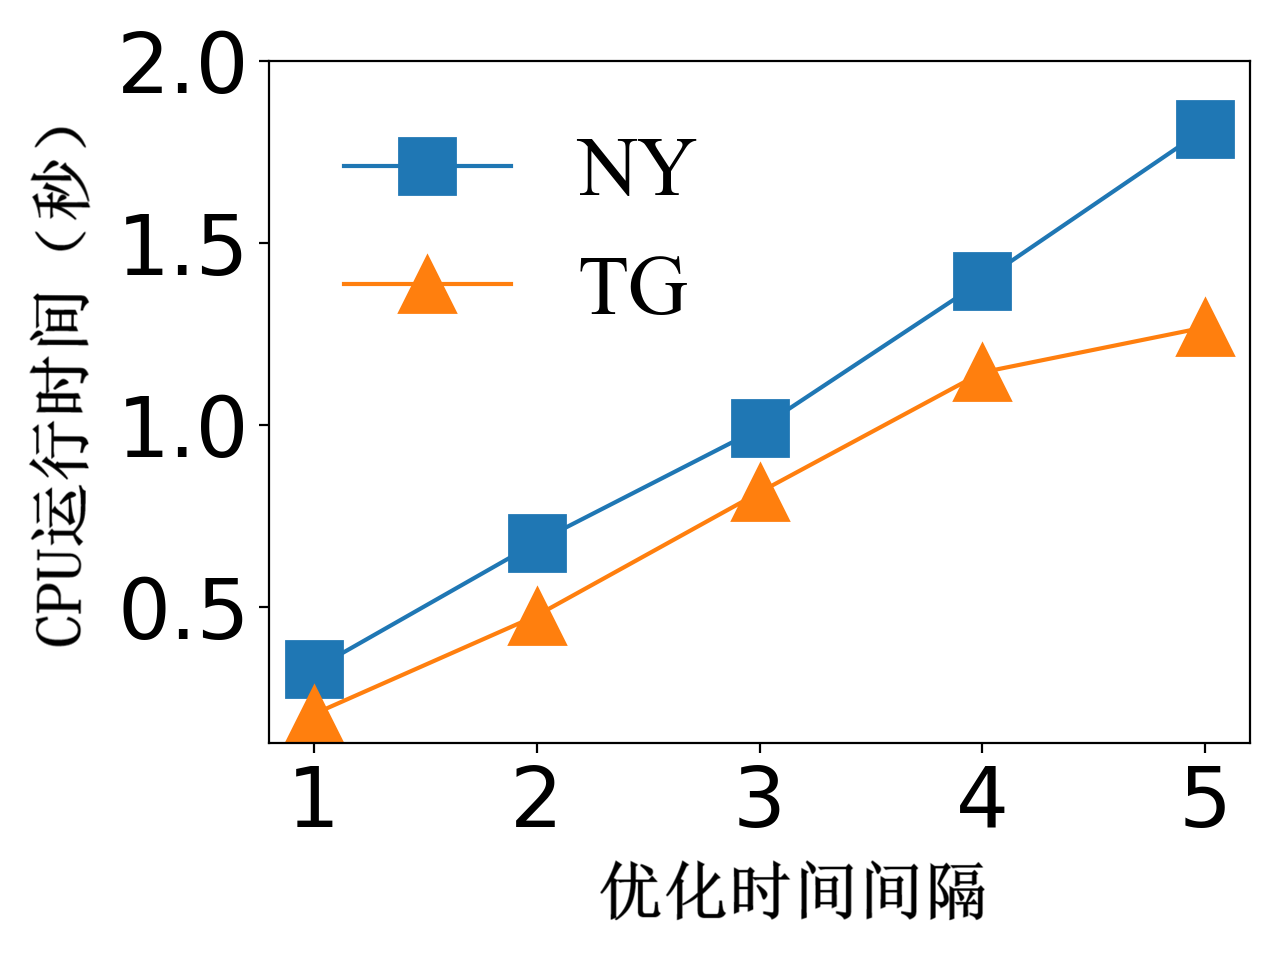
\includegraphics[width=0.4\linewidth]{fig/section3/fig4_time.png}
            \label{fig4:a}
        }% 
        \hfill
        \subfloat[Travel time]{
        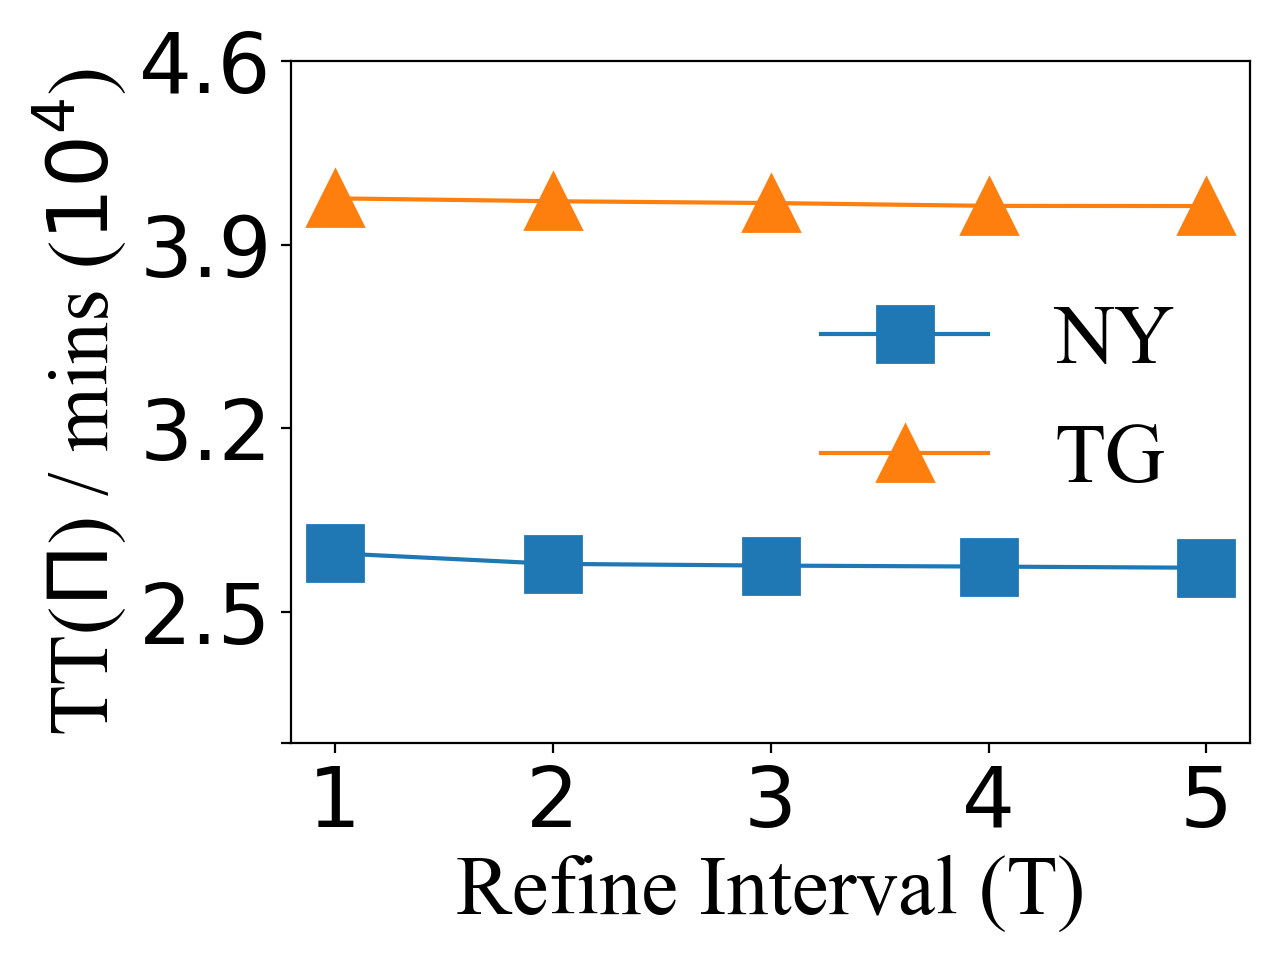
\includegraphics[width=0.4\linewidth]{fig/section3/fig4_cost.png}
            \label{fig4:b}
        }%
        \caption{批优化时间间隔T的影响}
        \label{fig4}
\end{figure*}

首先，在默认的参数设定下，我们调查了提出的算法在不同行程请求数目$|Q| $下的算法表现。直觉上，行程请求数目$ |Q| $越大，所有行程路线的总的通行时间会增加。此外，一个更大的$ |Q|$也会造成更大的计算消耗，CPU运行时间也会增加。图\ref{fig1}展示了我们提出的算法在TG路网和NY路网上的表现。意料之中的，随着行程请求数$|Q|$的增加，所有算法所需要的CPU时间都增加了。在这些算法中，基于个人的Ind算法需要的CPU时间最小，因为它是一次规划的，没有经过我们所提出的批优化处理这一过程。我们也同时发现Ind算法产生的全局路线组合中所有路线总的通行时间$TT(\Pi)$比其他算法更大，特别是在行程请求数目较大的情况下 (e.g., 当在NY路网中$|Q|=10,000$和在TG路网中 NY $|Q|=20,000$时, 和Ind算法比较，我们的SBP
算法能够减少超过40\%的通行时间).

和SBP算法相比，SBP*SA和SBP*DA表现较差。因为它们会在优化过程中进行较多次数的交换操作，这是非常耗时的。具体来说，SBP*SA没有考虑到已经规划的路线也会对路段交通增加额外的车流量，因此它在初始化路线搜索阶段进行的交通预测是不可靠的。对于SBP*DA算法，它以一个行程出发时刻的交通状态快照进行路径规划。因此，SBP*SA算法和SBP*DA算法所指定的初始化路线往往是低质量的，需要在批优化过程中采取大量的交换操作来对这些低质量的初始路线进行调整，从而产生了更多的计算消耗去提高结果质量。从图\ref{fig1:b}和图\ref{fig1:d}我们也观察到这三种算法产生的全局路线组合的所有路线的总的通行时间是非常接近的，而且我们的SBP算法总能产生较小的通行时间$TT(\Pi)$。这些实验结果证实了通过采用自感知的思想和考虑到网络动态性，我们的初始路线搜索能够有效地产生高质量的
处理路线，这样的初始路线可以减少后续优化处理过程中的交换操作次数。





\subsubsection{行程请求到达速率对算法效果的影响}
图\ref{fig2}展示了当行程请求到达速率发生改变时SBP算法的算法表现。行程请求到达速率越大，说明单位时间会有更多的车流涌入到路网的各个路段上。在这种情况下，每个路段车流量的增幅会更加明显。从而，每个路段上会产生更多的额外车流量。在图\ref{fig2}，观察CPU时间和总的通行时间$TT(\Pi)$，不管是在NY路网还是在TG路网上，我们都可以发现它们有明显的增长趋势。$TT(\Pi)$增长是因为随着车流量增加，每个路段的通行时间也相应增加了。在TG路网上，所有的行程规划的路线的总的通行时间远远大于在NY路网上的，这是因为在我们的默认设定中，TG路网会有更多数目的行程请求产生。




\subsubsection{通行时间函数各参数对算法效果的影响}
图\ref{fig3}展示了当我们变化通行时间函数中的参数$\alpha$和 $\beta$ (cf. 式 \ref{eq:tf})时SBP算法的算法表现。直觉上，$\alpha$越大或者$\beta$越小，各路段通行时间会增大，从而可能会加剧交通拥堵。在图\ref{fig3:a}中，当$\alpha$从1变化到5时，CPU时间和所有行程总的通行时间都有增加的趋势。相反的，当$\beta$从1变化到3时，总的通行时间具有下降的趋势。值得注意的是，当我们变化$\beta$时，CPU时间没有特别明显的变化趋势，这是因为CPU时间即我们所需要的计算消耗并不是和 $\beta$的值直接相关的。

\subsubsection{优化时间间隔对算法表现的影响}
图\ref{fig4}展示了当优化时间间隔$T$变化时SBP算法的表现。$T$越大代表着每个请求的等待时间增加了，但是规划的结果会更趋于最优，这是因为有更多的正在规划的路线被考虑到了对未来的交通状态影响中去了。在这种情况下，我们通过交换操作大大减少所有行程总的通行时间$TT(\Pi)$。在图\ref{fig4:a}，CPU时间随着$T$的增加而增加，这是因为我们在一次优化过程中需要处理更多的行程请求。在图\ref{fig4:b}中，我们可以发现$TT(\Pi)$有一个轻微的减小趋势。这些结果说明了一个合适的优化时间间隔能够通过重新利用已经规划的初始路线来更准确地未来的交通状态，从而避免交通拥堵。

\begin{figure}[h]
% 	Figure 1 effect Of Query Count
        \centering
        \subfloat[]{
            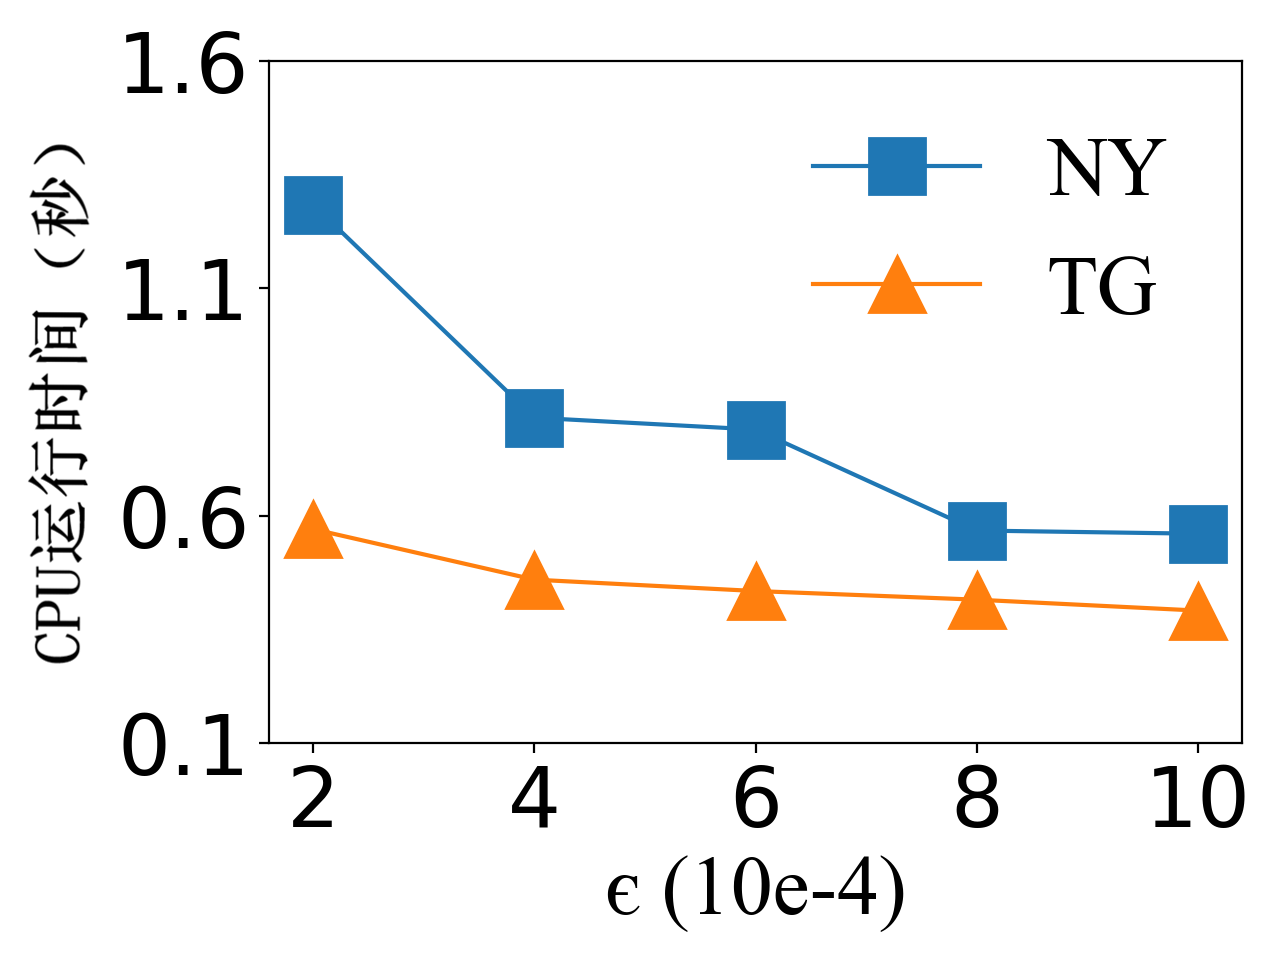
\includegraphics[width=0.33\linewidth]{fig/section3/fig5_time.png}
            \label{fig5:a}
        }%
        \subfloat[]{
            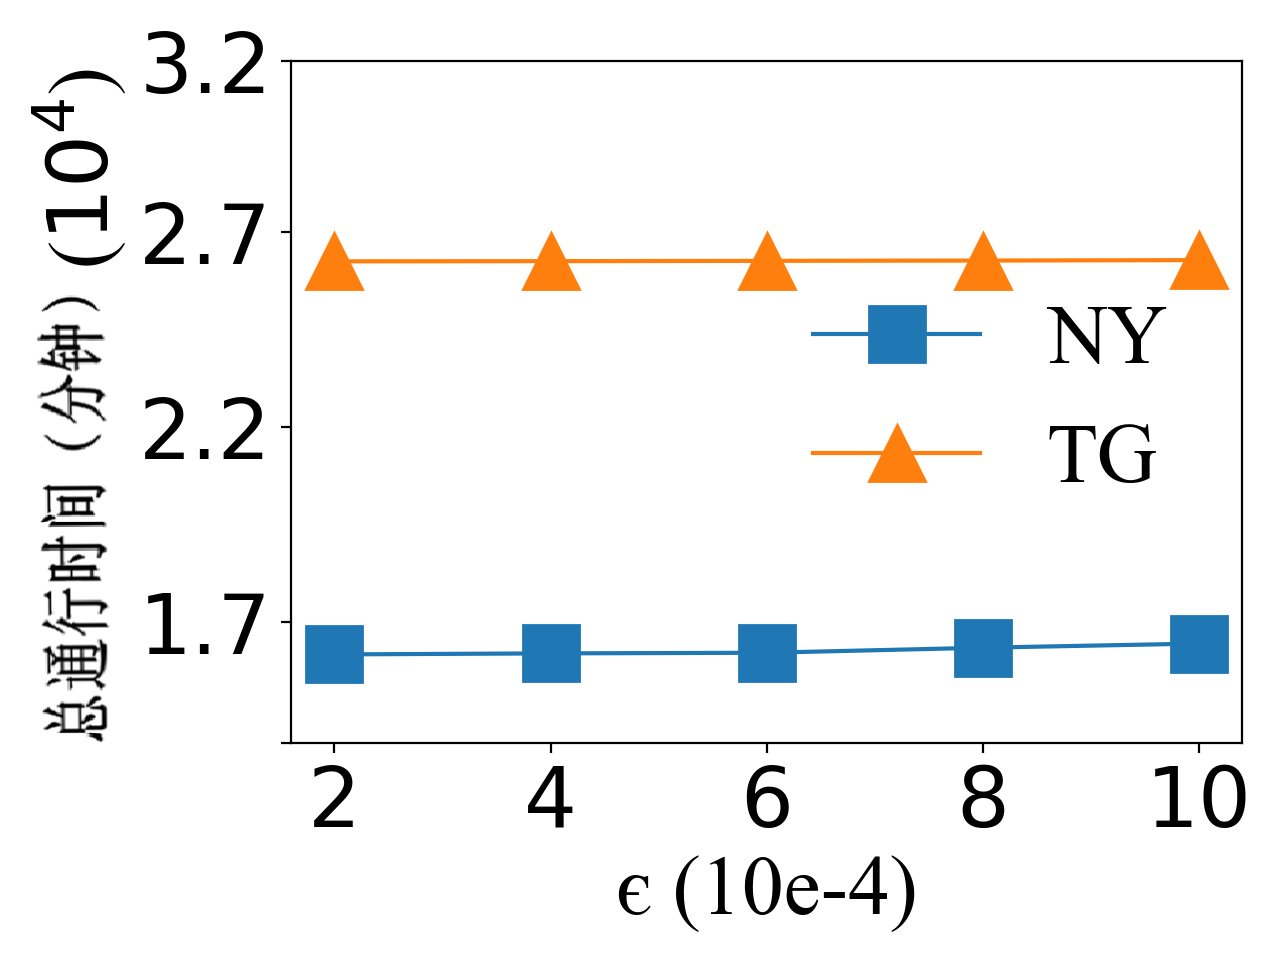
\includegraphics[width=0.33\linewidth]{fig/section3/fig5_cost.png}
            \label{fig5:b}
        }%
        \subfloat[]{
        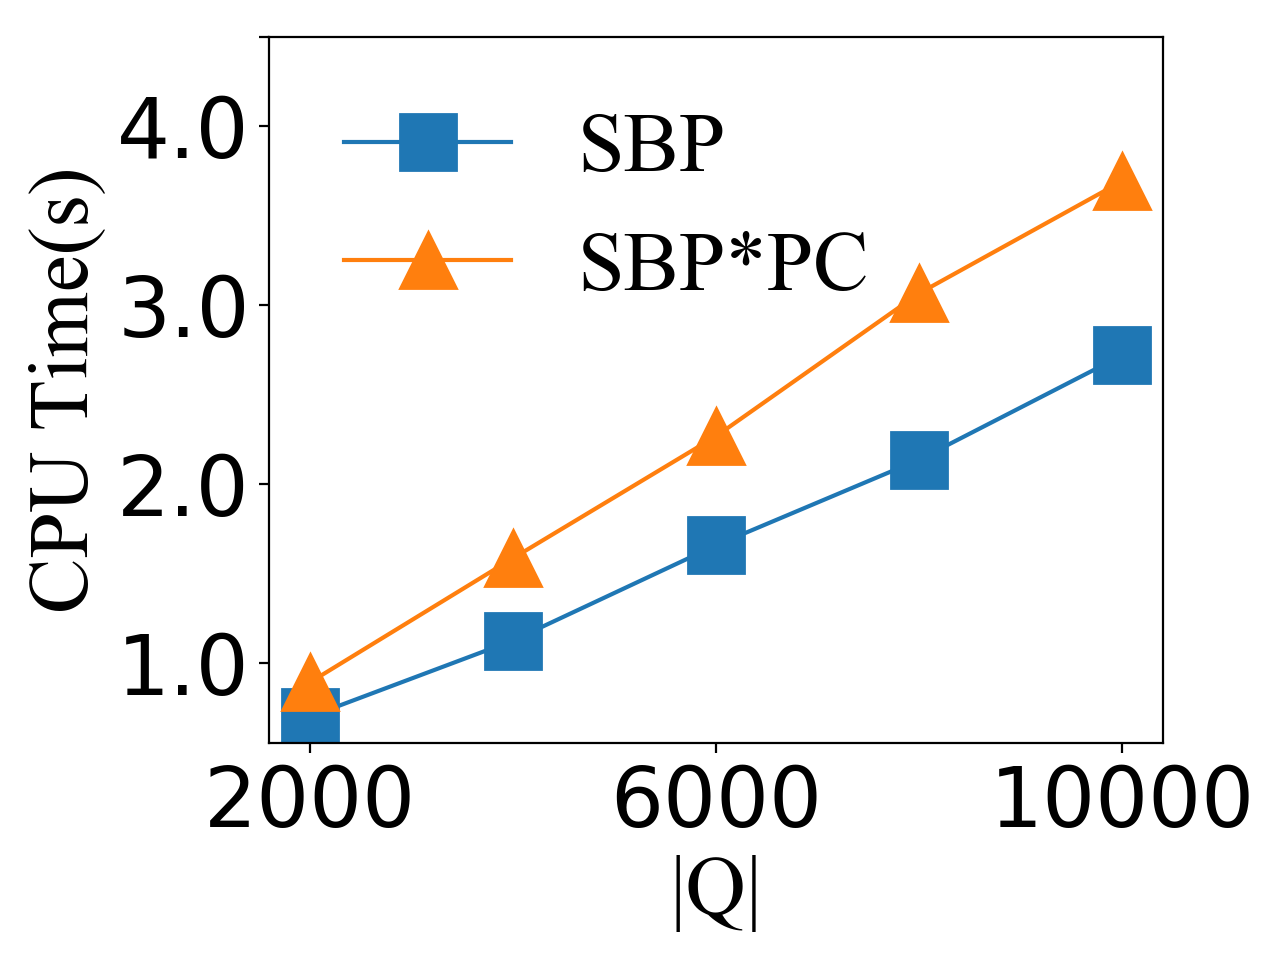
\includegraphics[width=0.33\linewidth]{fig/section3/fig6_NY.png}
            \label{fig5:c}
        }% 
        \caption{参数$\epsilon$和预检查策略的影响 \subref{fig5:a} CPU运行时间；\subref{fig5:b} 通行时间；\subref{fig5:a} 预先检查策略的影响评估 }
        \label{fig5}
\end{figure}

\subsubsection{参数$\epsilon$和预检查策略对算法表现的影响}
我们研究了当参数$\epsilon$从0.0002变化到 0.001时的SBP算法表现。我们知道在优化处理过程中，总的有效交换操作的次数是和参数$\epsilon$的值成反比的 (cf. 算法 \ref{alg:alg3})。$\epsilon$越大，意味着有效操作的门槛越高，有效操作的次数越少，因此CPU时间也会随之减少。然而，一个更大的$\epsilon$也会产生具有更大通行时间的全局路线组合$\Pi$。在图\ref{fig5:a}中，当参数$\epsilon$从0.0002变化到 0.001时，CPU时间有一个减少的趋势。
相反的，所有行程总的通行时间有一个轻微的增加的趋势。当$\epsilon$从0.0002 变化到0.0004时，所需要的CPU时间降幅最大 (e.g., 在NY路网和TG路网中，需要的CPU时间减少幅度分别超过了 36\% 和 19\%).  我们也发现对于$\epsilon$值的选取，0.001是非常合适的，从图中我们可以看出当$\epsilon$为0.001时，算法的综合表现是最好的。以上实验结果说明通过利用一个合适的参数$\epsilon$，SBP算法的表现能够得到较大的提升。 我们用"SBP*PC"来表示没有应用预检查策略的SBP算法，在图\ref{fig5:c}中，我们观察到SBP算法所需要的CPU运行时间总是比SBP*PC算法更少，这个实验结果说明了我们提出的预检查策略是能够进一步提升算法效率的。


\section{本章小结}
我们提出和调查了一个新颖的路线规划问题（CORC问题)，该问题旨在为持续的形成请求搜寻最佳的路线组合 。我们提出了一个SBP算法来高效解决CORC问题。同时，一些修剪枝技术的提出也大大提升了算法效率。对应的实验研究证实了我们提出的算法能够有效地解决该问题，也证实了我们提出的剪枝技术有够有助于避免不必要的计算。

	% \chapter{基于轨迹数据的群体联合移动模式挖掘}

\section{引言}
本章通过对大规模移动轨迹的系统分析，旨在设计高效且可扩展的算法框架，用于识别在特定时间区间内频繁共同出现在相邻空间位置，且在多个时间点存在联合移动的对象集合，即特定群体联合移动模式。该问题有助于为城市规划、交通管理以及社会行为研究等应用场景提供更加深入和精细化的决策支持。

为实现上述目标，本章从数据建模、索引结构设计与算法优化等多个层面展开研究。首先，对特定群体模式检测问题进行形式化定义，明确问题输入、输出及约束条件，并系统分析其在大规模数据环境下面临的计算复杂性与存储开销挑战；其次，结合时空数据挖掘技术，构建适用于大规模轨迹数据的高效索引结构，以支持高性能的候选模式生成与验证过程。在研究背景方面，调研了联合移动模式搜索与轨迹聚类领域的代表性工作，总结其在模式表达能力、计算效率与扩展性方面的优势与不足，从而引出本章研究的核心问题与技术挑战。在问题描述层面，本章依次给出了移动对象及其轨迹的形式化定义，刻画了协同行为的时间持续约束以及空间共现条件，并在此基础上提出了一个更加简化且具有实际意义的伴随群体发现问题定义。

总体而言，大规模性、模式定义的灵活性、算法效率要求以及数据动态变化特征共同构成了该问题的技术难点，也对算法框架设计与系统实现提出了更高要求。针对伴随群体发现问题，首先设计了一种精确求解算法，随后提出了一种新颖的社区感知聚类模型，返回近似解，以有效缩减搜索空间并提升候选群体的质量。基于两个真实世界数据集开展了全面的实验评估，实验结果表明，所提出的社区感知算法能够在用户可交互时间范围内，从大规模轨迹数据中高效发现伴随群体，验证了在实际应用场景中的可行性。

\subsection{研究背景与意义}

随着位置追踪设备，如车载导航系统和智能手机以及 GPS 智能服务的持续普及，轨迹数据的规模呈现爆炸式增长。作为时空数据挖掘中的一项核心任务，联合移动模式挖掘问题已受到广泛关注。一般而言，联合移动模式描述一组在一段时间内在空间上保持接近的对象集合。围绕这一问题，研究者提出了多种具有代表性的模式定义，包括 flock~\cite{DBLP:conf/gis/VieiraBT09,DBLP:journals/jidm/TanakaVK16}、convoy~\cite{DBLP:journals/pvldb/JeungYZJS08}、swarm~\cite{DBLP:journals/pvldb/LiDHK10}、group~\cite{DBLP:journals/dke/WangLH06}、platoon~\cite{DBLP:journals/dke/LiBK15} 以及 gathering~\cite{DBLP:conf/icde/ZhengZYS13,DBLP:journals/tkde/ZhengZYSZ14} 等。这些模式在时间连续性约束、空间密度约束以及成员稳定性等方面各有侧重，共同构成了联合移动模式研究的理论基础。

在诸多实际应用中，高效且准确地从移动对象轨迹中发现联合移动模式具有重要意义。例如，在拼车推荐与出行规划中，可以通过识别稳定的同行群体，使其共同出发或考虑彼此对交通的影响等，从而提升资源利用率；在交通拥堵缓解中，可通过及早发现道路上的高密度移动群体来规避潜在拥堵；在新冠病毒等传染病的暴露与风险分析中，可辅助识别潜在高风险接触群体~\cite{imo,DBLP:journals/information/AlarabiBHA21}；此外，在移动行为分析与异常轨迹检测~\cite{DBLP:conf/icde/Liu0CB20} 等任务中，群体模式挖掘同样发挥着关键作用。

然而，如何在保证模式表达能力的同时提升计算效率，成为该领域亟需解决的重要问题。现有研究大多基于移动对象随时间演化的完整轨迹设计搜索算法。这类方法通常在每一个时间快照上执行聚类或密度计算，以判断对象之间的空间邻近关系。当联合移动模式在时间上不稳定，即对象可能暂时离开群体后又重新加入时，算法需要反复进行候选生成与验证，计算代价显著增加。尤其是在实时或近实时应用场景中，对所有时间快照进行全量聚类将带来极高的时间开销。此外，主流方法多采用“过滤–精炼”的处理框架，在过滤阶段通过建立时空索引排除不可能的数据对象，仅保留可能的候选群体，再在精炼阶段逐一验证其有效性。随着轨迹数据规模的持续增长，候选数量呈指数级膨胀，导致算法性能显著下降，难以满足大规模与在线分析的需求。



\subsection{研究内容与挑战}
在现实应用中，尤其是在公共安全紧急预警与传染病防控等对时效性要求极高的场景下，及时获得最新的联合移动结果至关重要。因此，联合移动模式挖掘任务往往需要以连续或增量的方式执行。这不仅要求算法在时间复杂度上具备良好的可扩展性，还要求其在模式定义上具有一定的灵活性，以适应动态变化的移动行为。然而，现有群体模式定义及其对应方法在同时兼顾模式表达能力与计算效率方面仍存在明显不足，难以在大规模数据环境中实现高效、稳定的持续挖掘。

为了解决上述问题，本文提出了一种联合移动模式概念——伴随群体。相较于已经存在的传统的联合移动模式定义，伴随群体的约束更加宽松且更具实用性。具体而言，一个伴随群体由至少 $m$ 个移动对象组成，这些对象需要在至少 $k$ 个时间段内在空间上保持接近（例如，两两距离不超过预定义的距离阈值 $\epsilon$），并允许对象在时间维度上暂时离开群体而不破坏整体模式的有效性。基于该模式定义，进一步形式化提出了伴随群体发现问题。给定一组移动对象及其轨迹数据，伴随群体发现问题旨在在用户可交互时间范围内高效发现所有满足条件的伴随群体。此外，在问题设定中，若某一对象能够同时参与多个伴随群体，则将其归属于成员规模最大的伴随群体，以保证群体划分结果的确定性与可解释性。伴随群体发现问题问题具有广泛的应用前景，可服务于交通监测与管理、疫情防控、公共安全预警以及群体行为分析等多种实际场景，为大规模时空数据环境下的群体行为挖掘提供一种高效且可扩展的解决方案。

\begin{figure}[htbp]
    \centering
    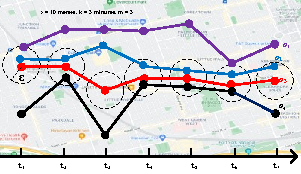
\includegraphics[width=1\textwidth]{fig/section4/group companion.pdf}
    \caption{伴随群体发现问题示例}
    \label{cm_fig:intro}
\end{figure}

\begin{example}[伴随群体发现问题示例]
图~\ref{cm_fig:intro}给出了一个具体示例以直观说明伴随群体的判定过程。设 $o_1, o_2, o_3, o_4$ 为四个移动对象，且所有对象以固定采样频率每分钟上报一次位置信息。图~\ref{cm_fig:intro} 展示了这四个移动对象在时间区间 $[t_1, t_7]$ 内的轨迹变化情况。设空间距离阈值为 $\epsilon = 10$ 米，联合移动的最小持续时间阈值为 $k = 3$，群体规模阈值为 $m = 3$。首先，从对象两两关系的角度进行分析。可以观察到，对象 $o_2$ 与 $o_3$ 在时间集合 $T = \{t_1, t_2, t_4, t_5, t_6, t_7\}$ 内始终满足两两距离不超过 $\epsilon$ 的约束，即在这些时间点保持空间接近关系。由于 $|T| = 6$，显著超过持续时间阈值 $k$，因此 $o_2$ 与 $o_3$ 构成一个满足条件的联合移动对。同理，$o_3$ 与 $o_4$ 在不少于 $k$ 个时间点内保持空间邻近关系，也可以构成一个联合移动对。在此基础上，进一步考察多对象群体关系。可以发现，在时间点 $\{t_2, t_4, t_5, t_6\}$ 上，对象 $o_2, o_3, o_4$ 的两两距离均不超过 $\epsilon$，即它们在这些时间点形成一个空间上连通且满足密度约束的三元对象集合。由于该时间集合的规模不少于持续时间阈值 $k$，且群体规模 $|g| = 3$ 满足最小规模阈值 $m$，因此将 $g=\{o_2, o_3, o_4\}$ 判定为一个有效的伴随群体。需要注意的是，对象 $o_1$ 仅在 $t_1$ 和 $t_6$ 与 $o_2$ 短暂接近，其满足距离约束的时间点数量不足以达到持续时间阈值 $k$，且未能与其他对象形成稳定的多对象联合移动模式。因此，$o_1$ 既无法与其他对象构成有效的联合移动对，也不能参与任何满足条件的伴随群体。该示例说明，伴随群体的判定不仅依赖于空间邻近关系，还同时受到时间持续性与群体规模约束的共同影响，从而能够更全面地刻画移动对象之间的协同行为特征。
\end{example}
为了高效解决伴随群体发现问题，系统在算法设计与工程实现层面面临多方面的关键技术挑战，这些挑战既来源于数据本身的规模与动态特性，也源于模式定义的复杂性与计算代价。具体而言，主要包括以下几个方面：

\begin{itemize}
    \item \textbf{大规模数据处理：}在真实应用场景中，轨迹数据通常来源于海量移动对象，例如车辆、移动终端或各类传感设备，其数据规模可能达到千万级甚至更高。轨迹数据不仅记录频繁，而且具有高维度与强相关性特征，使得存储与计算开销显著增加。如何在如此庞大的数据规模下实现高效的数据组织、索引构建与查询处理，尤其是在需要实时或近实时发现群体模式的场景中，成为首要挑战。这不仅要求算法具备良好的时间复杂度和可扩展性，还需要设计紧凑的空间组织结构与高效的内存管理策略，以降低存储成本并减少 I/O 开销。

    \item \textbf{模式定义的灵活性：}不同应用场景对群体模式的语义需求存在差异。例如，有的应用更关注空间邻近性，有的强调时间持续性，还有的关注成员规模或运动一致性等约束条件。因此，如何构建一个既支持多种群体模式表达，又能够灵活调整参数（如距离阈值、持续时间阈值与最小群体规模）的统一算法框架，是实现方法广泛适用性的关键。同时，该框架在增强表达能力的同时，必须避免因模式定义过于复杂而导致搜索空间急剧膨胀，从而影响整体计算效率。

    \item \textbf{准确性与效率的平衡：}群体模式发现通常涉及复杂的时空约束匹配、多对象关系维护以及候选结构验证等操作。若直接采用精确枚举算法，往往需要在大量时间快照上反复执行聚类或连通性检测，计算代价极高。因此，如何在保证结果准确性的前提下，通过有效的剪枝策略、搜索空间压缩技术、分层索引机制或近似计算方法减少不必要的候选生成与验证，是提升系统性能的核心问题。尤其在数据规模持续增长的背景下，算法必须在结果质量与运行效率之间取得合理且可控的权衡。

    \item \textbf{动态性的处理：}轨迹数据具有天然的动态特征，移动对象的位置与行为随时间持续变化。在流式或持续更新的数据环境中，新轨迹不断到达，历史数据逐渐失效，群体结构也随之演化。若每次更新都重新对全部历史数据进行计算，将带来难以接受的时间开销。因此，如何设计支持增量更新或滑动窗口处理机制的算法，在无需重复计算全部数据的前提下高效维护群体模式结果，是保证系统实时性、稳定性与可扩展性的关键技术挑战。
\end{itemize}

\subsection{研究成果与贡献}
综上所述，大规模数据处理需求、模式定义的灵活性要求、算法效率约束以及数据动态演化特征，共同构成了伴随群体发现问题的核心技术难点，也对整体算法框架设计与系统实现提出了更高要求。针对伴随群体发现问题，本文从精确算法设计与高效近似算法设计两个层面展开研究。

首先，设计了一种精确搜索算法。该算法基于严格的时空约束判定机制，对候选对象对及候选群体进行精确验证，能够保证结果的完备性与准确性。然而，由于需要在多个时间维度上进行精细化匹配与验证，其计算代价相对较高，更适用于离线分析或数据规模适中的场景。

为进一步提升算法效率并满足实时或近实时应用需求，本文额外提出了一种社区感知的近似搜索算法。该算法在保证结果质量可控的前提下，通过近似计算与结构化聚类方法显著压缩搜索空间，从而在严格的效率约束下有效解决伴随群体发现问题，实现准确性与效率之间的平衡。

近似算法主要包括两个阶段：近似联合移动对搜索阶段与社区感知群体发现阶段。在近似联合移动对搜索阶段，首先采用基于网格划分的空间离散化方法，将每个轨迹位置映射为对应的网格单元编号，从而将连续轨迹转换为离散的网格单元编号序列表示。随后，通过计算不同轨迹之间的公共编号数量来快速估计其潜在的联合移动程度，从而生成候选的近似联合移动对。该过程有效避免了在原始连续空间中进行高代价的距离计算。在社区感知群体发现阶段，将生成的联合移动对视为图结构中的边，并利用 SCAN 算法~\cite{DBLP:conf/kdd/XuYFS07} 进行结构化聚类，以识别具有高内聚性和清晰社区边界的对象集合。通过引入社区结构约束，算法能够在保证群体结构合理性的同时，进一步降低无效候选的数量，从而提升整体运行效率。本文算法实现已开源发布\footnote{https://github.com/Like-China/gathering\_mining.git}，以便于后续研究复现与扩展。

本文的主要贡献总结如下：
\begin{itemize}
    \item 提出了伴随群体这一联合移动模式定义。该定义相较于传统模式更加宽松且具备更强的适应性，尤其适用于需要持续结果更新与快速响应的应用场景，例如传染病传播监测与公共安全紧急风险预警。
    \item 设计并实现了一种精确搜索算法以及一种社区感知的近似搜索算法，系统性地解决了伴随群体发现问题在准确性与效率之间的权衡难题。
    \item 基于两个真实世界数据集开展了全面的实验评估。实验结果表明，所提出的社区感知算法能够在用户可交互时间范围内，从大规模轨迹数据中高效发现伴随群体，验证了方法在实际应用场景中的有效性与实用价值。
\end{itemize}

本文其余部分组织结构如下。第~\ref{cm_sec:problem} 节首先形式化给出问题定义，并介绍相关的符号说明与必要的预备知识，为后续算法设计奠定理论基础。第~\ref{cm_sec:exact} 节在此基础上提出一种精确算法，详细阐述其核心思想、实现流程以及时间复杂度分析。第~\ref{cm_sec:approximate} 节进一步给出一种社区感知的高效近似算法，通过结构压缩与候选剪枝策略提升算法的可扩展性，并分析其性能优势与适用场景。第~\ref{cm_sec:exp} 节基于真实世界轨迹数据开展系统实验，从有效性与效率两个方面对所提方法进行全面评估与对比分析。最后，第~\ref{cm_sec:conclusion} 节对全文进行总结，并展望未来的研究方向。

\section{问题定义}
\label{cm_sec:problem}

本节介绍所需的基础概念，并给出问题的形式化定义。给定一组移动对象，依次定义移动对象及其轨迹、协同行为持续时间、协同行为对、伴随群体以及伴随群体发现问题。本章所使用的主要符号及其解释如表\ref{cm_tab:notation}所示。

\begin{table}[htbp]
    \centering
    \setlength{\tabcolsep}{8pt}% column separation
    \caption{主要符号解释}
    \label{cm_tab:notation}
    \renewcommand{\arraystretch}{1}%row space 
    \begin{tabular}{ll}
        \hline
		\bfseries 符号 & \bfseries 解释 \\
        \hline
        $o$ & 一个移动对象\\
        $O$ & 一组移动对象集合\\
        $s$ & 一个采样位置点\\
        $\tau$ & 一条轨迹 \\
        $\mathcal{T}$ & 一组轨迹集合\\
        $t$ & 某个时刻\\
        $\epsilon_s$/$\epsilon_t$ & 空间距离阈值/时间距离阈值\\
        $k$ & 协同行为持续时间阈值\\
        $m$ & 最小群体规模阈值 \\
        $g$ &一个伴随群体\\
        $\mathcal{G}$ & 一组伴随群体 \\
        \hline
    \end{tabular}
\end{table}

\begin{definition}[移动对象及其轨迹]
一个移动对象 $o$ 由其轨迹 $\tau=\{s_1,\ldots,s_n\}$ 表示，其中轨迹是一个有限的、按时间顺序排列的离散时空点序列。该序列由位置追踪设备从对象 $o$ 的真实运动轨迹中采样获得。

为简化描述，使用 $s_i=([x,y],t)$ 表示二维空间中的一个离散采样位置点，其中 $[x,y]$ 表示空间坐标，$t$ 表示该位置被记录时对应的时间戳。对于一组移动对象 $O$，记其轨迹集合为 $\mathcal{T}=\{\tau_1,\ldots,\tau_{|O|}\}$，其中 $\tau_i$ 为对象 $o_i$ 的轨迹。本文对移动对象及轨迹的建模方式与已有研究保持一致~\cite{DBLP:conf/ijcai/LiCSWLK022,DBLP:conf/icde/RanuPTDR15,DBLP:conf/sigmod/SuZWHZ13}。
\end{definition}

\begin{definition}[协同行为持续时间]
设 $o_i$ 与 $o_j$ 为两个移动对象。当 $o_i$ 与 $o_j$ 之间的空间距离小于等于给定的空间距离阈值 $\epsilon_s$，且对应时间戳之差不超过给定的时间距离阈值 $\epsilon_t$ 时，称二者在该时刻处于协同行为状态。对象 $o_i$ 与 $o_j$ 的协同行为持续时间定义为所有满足上述条件的时间长度之和。
\end{definition}

\begin{definition}[协同行为对]
设 $\tau_i$ 与 $\tau_j$ 分别为对象 $o_i$ 与 $o_j$ 的轨迹。给定$k$ 为协同行为持续时间阈值，若 $\tau_i$ 与 $\tau_j$ 之间的协同行为持续时间不少于给定阈值 $k$，则称对象 $o_i$ 与 $o_j$ 构成一个协同行为对。
\end{definition}

\begin{definition}[伴随群体]
给定一组移动对象 $\mathcal{O}=\{o_1,o_2,\ldots,o_{|\mathcal{O}|}\}$ 以及最小群体规模阈值 $m$，若对象子集 $g\subseteq \mathcal{O}$ 满足以下两个条件，则称 $g$ 为一个伴随群体：
\begin{enumerate}
    \item $|g|\geq m$；
    \item 对任意两个对象 $o_i,o_j\in g$，$o_i$ 与 $o_j$ 均构成协同行为对。
\end{enumerate}
\end{definition}

\begin{definition}[伴随群体发现问题]
给定一组移动对象 $\mathcal{O}$，伴随群体发现问题旨在从 $\mathcal{O}$ 中发现一组伴随群体 $\mathcal{G}$，并满足对任意两个群体 $g_i, g_j\in\mathcal{G}$，均有 $g_i\cap g_j=\emptyset$。
\end{definition}

\section{精确搜索算法}
\label{cm_sec:exact}

本节提出一种用于发现伴随群体的精确求解方法——精确联合移动算法（\underline{E}xact \underline{S}earch with \underline{E}xact \underline{C}o-\underline{M}ovement \underline{C}omputation，简称 ES-ECMC）。该算法对所有候选对象组合进行精确验证，从而保证结果的完备性与正确性。

ES-ECMC 算法整体上包含三个核心步骤。首先，给定输入数据，即一组移动对象轨迹集合，通过精确的时空约束计算枚举并识别所有满足持续时间阈值 $k$ 的联合移动对；其次，以这些联合移动对为基础，构建对象之间的关联结构，并采用增量扩展策略逐步生成满足条件的伴随群体候选；最后，在所有生成的候选集合中，依据成员规模优先的原则筛选出不可扩展且规模最大的伴随群体作为最终输出结果。该三阶段流程分别对应“协同行为对发现—伴随群体候选集合扩展—结果筛选”三个层次，层层递进，从而实现对搜索空间的系统化遍历与剪枝。在介绍具体流程之前，首先给出伴随群体候选的形式化定义，以便后续算法描述与性质分析。

\begin{definition}[伴随群体候选]
一个伴随群体候选 $g'$ 是一个对象集合，满足其中任意两个对象均可以构成一个联合移动对。若存在至少一个集合外的对象 $o \notin g'$，使得扩展后的集合 $g' \cup \{o\}$ 仍然满足上述条件，则称 $g'$ 可以通过加入对象 $o$ 进行扩展；否则，称 $g'$ 为不可扩展的伴随群体候选。
\end{definition}


\begin{algorithm}[htbp]
    \caption{ES-ECMC}
    \label{cm_alg:S-ECMC}
    \Input{轨迹集$\mathcal{T}=\{\tau_1,\tau_2,\ldots,\tau_{|\mathcal{O}|}\}$;\newline
    空间距离阈值 $\epsilon_s$;\newline
    时间距离阈值 $\epsilon_t$;\newline
    群体规模阈值 $m$;\newline
    联合移动持续时间阈值 $k$。
    }
    
    \Output{一组满足定义约束的精确的伴随群体集合 $G$。}
    
    \BlankLine
    初始化：$P \leftarrow \emptyset$;\tcp*[f]{有效轨迹对集合}

    初始化：$G_c \leftarrow \emptyset$;\tcp*[f]{候选群体集合}

    初始化：$G \leftarrow \emptyset$;\tcp*[f]{最终结果集合}
    
    \BlankLine
    \For(\tcc*[f]{生成有效轨迹对}){$i = 1$ \KwTo $|\mathcal{T}|$}{
        \For{$j = i+1$ \KwTo $|\mathcal{T}|$}{
            \If{$|\tau_i \cap \tau_j| \ge k$}{
                $P \leftarrow P \cup \{(\tau_i,\tau_j)\}$;
            }
        }
    }
    
    \BlankLine
    \ForEach(\tcc*[f]{扩展候选群体}){$(\tau_i,\tau_j) \in P$}{
        $g_i \leftarrow \{\tau_i,\tau_j\}$;
    
        \ForEach{$(\tau_i,\tau_k) \in P$}{
            \If(\tcc*[f]{两两有效且所有成员均在 $g_i$ 中})
            {$\forall \tau_p \in g_i,\; (\tau_k,\tau_p) \in P$}{
                $g_i \leftarrow g_i \cup \{\tau_k\}$;
            }
        }
    
        \If(\tcc*[f]{群体规模约束}){$|g_i| \ge m$}{
            $G_c \leftarrow G_c \cup \{g_i\}$;
        }
    }
    
    \BlankLine
    $G \leftarrow select\_max(G_c)$;\tcp*[f]{选择最大或最优群体}
    
    \Return $G$;
\end{algorithm}


下面将详细介绍 ES-ECMC 算法的整体流程与核心思想。算法~\ref{cm_alg:S-ECMC} 给出了 ES-ECMC 的完整伪代码描述。该算法以一组轨迹数据 $\mathcal{T}$ 作为输入，同时给定空间距离阈值 $\epsilon_s$、时间距离阈值 $\epsilon_t$、最小群体规模阈值 $m$ 以及联合移动持续时间阈值 $k$。算法的输出为一组满足定义约束的伴随群体集合
$G=\{g_1,g_2,\ldots\}$，其中每个 $g_i \subseteq \mathcal{T}$，表示由若干移动对象轨迹构成的一个伴随群体。在实现层面，使用一个集合 $P$ 存储所有满足持续时间阈值 $k$ 的协同行为对，用以刻画对象之间的两两联合移动关系 （第1行）；同时，使用一个集合 $G_c$ 存储在搜索过程中生成的伴随群体候选 （第2行）。通过先构建联合移动对集合 $P$，再基于 $P$ 进行增量式候选扩展与验证，算法能够系统地遍历可能的对象组合，并通过可扩展性判定与规模约束进行有效剪枝，从而最终得到满足条件的伴随群体集合 $G$ （第3行）。该算法包含3个主要步骤：枚举联合移动对，生成伴随群体候选，以及选择伴随群体。

    \underline{步骤 1：}（枚举联合移动对）

    对于任意一对移动对象 $o_i, o_j \in \mathcal{O}$，计算其轨迹中任意两个采样位置
    $s \in \tau_i$ 与 $s' \in \tau_j$ 之间的精确距离。若空间距离与时间距离分别不超过阈值 $\epsilon_s$ 与 $\epsilon_t$，则将其联合移动持续时间 $|\tau_i \land \tau_j|$ 累加 1。具体而言，对于每一对对象 $\langle o_i,o_j\rangle$，当其累计的联合移动持续时间不少于阈值 $k$ 时，将其视为一个联合移动对\footnote{在上下文清晰的情况下，使用 $(o_i,o_j)$ 或 $(\tau_i,\tau_j)$ 表示一个联合移动对。}。当所有对象对均被评估完成后，该步骤结束（第 4--7 行）。
    
    \smallskip
    \underline{步骤 2：}（生成伴随群体候选）
    
    在获得所有联合移动对之后，基于这些联合移动对以增量方式生成伴随群体候选。具体而言，首先选择一个以轨迹 $\tau_i$ 为起点的联合移动对，例如 $\langle \tau_i,\tau_j\rangle$，然后考察所有与其共享对象 $o_i$ 的联合移动对 $\langle \tau_i,\tau_k\rangle$。初始群体记为 $g_i=\{\tau_i,\tau_j\}$。若 $\tau_k$ 与 $g_i$ 中的所有成员均构成联合移动对，则将 $\tau_k$ 加入 $g_i$。当 $g_i$ 仍可扩展时，重复上述扩展过程。若 $|g_i| \ge m$，则将其加入候选集合 $G_c$。随后选择新的联合移动对作为初始群体并继续扩展。当所有联合移动对均被访问并作为初始群体尝试扩展后，该步骤结束（第 8--14 行）。
    
    \smallskip
    \underline{步骤 3：}（选择伴随群体）
    
    在获得所有候选群体之后，从中选取成员规模最大的伴随群体作为最终结果。具体而言，若某个对象同时属于多个候选群体，则仅保留其中成员规模最大的一个。该步骤在遍历完所有候选群体后结束（第 15 行）。
    
    \begin{example}[ES-ECMC算法示例]
    再次考虑图~\ref{cm_fig:intro} 中的示例。假设首先选择联合移动对 $\langle o_2,o_3\rangle$ 进行扩展。显然，联合移动对 $\langle o_2,o_4\rangle$ 与 $\langle o_2,o_3\rangle$ 共享对象 $o_2$，且对象 $o_2,o_3,o_4$ 两两之间均可形成联合移动对。因此，将 $g'=\{o_2,o_3,o_4\}$ 视为一个伴随群体候选。由于对象 $o_1$ 无法与 $g'$ 中的任一对象形成联合移动对，$g'$ 不可进一步扩展。接着，由于 $|g'|$ 不小于预设的群体规模阈值 3，将 $g'$ 加入候选集合 $G_c$。最终，由于 $g'$ 具有最大的成员规模，从 $G_c$ 中选取 $g'$ 并将其加入结果集合 $G$。
    \end{example}



    \begin{theorem}[ES-ECMC 算法时间复杂度]
    ES-ECMC 算法的时间复杂度为 $O(|\mathcal{T}|^2 \times |\tau|^2)$，其中 $|\mathcal{T}|$ 表示移动对象或轨迹的数量，$|\tau|$ 表示单条轨迹的平均长度，即采样位置数。
    \end{theorem}
    
    \begin{proof}
    ES-ECMC 的主要时间开销来自三个阶段。
    
    首先，在枚举所有联合移动对时，需要对任意一对轨迹 $\tau_i,\tau_j \in \mathcal{T}$ 进行逐点比较。对于每一对轨迹，需计算其所有采样点对之间的空间距离与时间距离，时间复杂度为 $O(|\tau|^2)$。由于轨迹对的数量为 $O(|\mathcal{T}|^2)$，因此该阶段的总体时间复杂度为
    \[
    O(|\mathcal{T}|^2 \times |\tau|^2)。
    \]
    
    其次，在生成伴随群体候选阶段，对于共享同一对象的联合移动对（例如 $\langle o_i,o_j\rangle$ 与 $\langle o_i,o_k\rangle$），需要判断其是否能够构成伴随群体候选，并在满足条件时进行扩展。该过程本质上是在联合移动对构成的图结构上进行增量式团扩展。最少情况下（例如不存在任何共享对象的联合移动对），该阶段仅需线性扫描联合移动对集合，时间复杂度为 $O(|\mathcal{T}|)$；在最坏情况下，若任意两个对象之间均可形成联合移动对，则候选生成过程可能涉及 $O(|\mathcal{T}|^2)$ 次组合与验证操作。然而，该阶段的复杂度上界仍然不超过前一阶段的 $O(|\mathcal{T}|^2 \times |\tau|^2)$。
    
    最后，在候选集合 $G_c$ 中选择最终伴随群体时，仅需遍历所有候选并进行规模比较，时间复杂度为 $O(|G_c|)$。由于 $|G_c| < |\mathcal{T}|^2$，且通常远小于前两阶段的计算规模，因此该阶段不会改变整体复杂度阶。
    综上所述，ES-ECMC 算法的总体时间复杂度由联合移动对枚举阶段主导，为
    \[
    O(|\mathcal{T}|^2 \times |\tau|^2)。
    \]
    \end{proof}


\section{基于近似协同行为计算的社区感知搜索}
\label{cm_sec:approximate}

尽管 ES-ECMC 精确算法直观且能够保证结果的精确性，但其较高的计算开销使其难以直接应用于大规模实际场景，尤其是在移动对象数量极大的情况下。其主要性能瓶颈在于需要通过精确计算协同行为持续时间来枚举所有协同行为对，该过程涉及大量轨迹间的逐点比较操作，时间代价高昂。为提升算法效率，本文提出一种基于社区感知的搜索算法，并结合近似协同行为计算策略，即 \underline{C}ommunity-aware \underline{S}earch with \underline{A}pproximate \underline{C}o-\underline{M}ovement \underline{C}omputation（简称 CS-ACMC）。该方法在保证较高结果质量的同时，显著降低了计算复杂度。CS-ACMC 算法主要包含两个阶段：（1）近似协同行为对搜索阶段，通过构建轨迹的紧凑表示并进行快速相似性筛选，以高效识别潜在的协同行为对；（2）基于社区感知的聚类阶段，在所构建的对象关系图上挖掘结构紧密的对象子集，从而获得伴随群体。接下来，将依次介绍近似协同行为对搜索策略以及社区感知聚类算法的具体设计。

\subsection{近似协同行为对搜索}

在该阶段中，提出了一种高效的协同行为对搜索方法，用于计算两个对象轨迹之间协同行为持续时间的近似值。所生成的近似协同行为对将作为后续社区感知聚类阶段的输入，从而高效地发现伴随群体。该阶段包含两个子步骤：生成轨迹网格编号序列，以及搜索近似协同行为对。

\subsubsection{轨迹网格编号序列生成}

该方法受到群体（flock）圆形结构思想的启发 \cite{DBLP:journals/pvldb/JeungYZJS08}。首先将底层时空域进行离散化处理：在空间维度上，将二维欧氏空间划分为边长相等的网格单元；在时间维度上，将时间轴划分为等长的时间片。因此，对于对象轨迹中的每一个数据点（位置）$s=([x,y],t)$，均可映射为一个网格编号，记为
$o(s)=f(x,y,t)$，
其中 $f(\cdot)$ 为单射函数，用于将三维离散坐标唯一映射为一个整数标识。由此，轨迹 $\tau$ 可表示为对应的网格编号序列：
$
O(\tau)=\{o(s_1),\ldots,o(s_{|\tau|})\}
$。图 \ref{cm_fig1:cell_partition} 展示了空间与时间维度的划分方式以及轨迹网格编号序列的生成过程。假设空间被划分为 $5\times 4$ 个网格单元，每个单元边长为 10 米，时间维度被划分为 3 个时间片，每个时间片长度为 10 秒。给定两条轨迹 $\tau_1$ 和 $\tau_2$，其位置分别落入单元
$\{([0,0],0), ([3,1],1), ([2,1],2)\}$。基于上述划分方式，定义单射函数为
$o(s)=f(x,y,t)=t\times(5\times4)+y\times5+x$，
其中 $x\in\{0,1,2,3,4\}$，$y\in\{0,1,2,3\}$，$t\in\{0,1,2\}$。
\begin{example}
    对于位置 $([3,1],1)$，其网格编号值为$1\times(5\times4)+1\times5+3=28$。如图 \ref{cm_fig1:cell_partition} 所示，尽管 $\tau_1$ 与 $\tau_2$ 在各时间点的精确空间位置不同，但由于它们落入相同的空间网格单元与时间片，因此可被表示为相同的网格编号序列 $\{0, 28, 47\}$。
\end{example}


\begin{theorem}
若将空间划分为边长为 $\epsilon$ 的等大小网格单元，其中 $\epsilon$ 等于协同行为距离阈值，则若两个对象 $o_i$ 与 $o_j$ 的轨迹网格编号序列共享 $p$ 个相同网格编号，则它们的协同行为持续时间至少为 $p$ 个时间段。
\end{theorem}

\begin{proof}
位置 $s$ 的网格编号值由单射函数 $o(s)=f(x,y,t)$ 唯一确定。若两个位置具有相同的网格编号值，则说明它们位于同一个空间网格单元，并且处于同一时间片内。由于网格单元的边长设置为协同行为距离阈值 $\epsilon$，因此同一单元内任意两点之间的空间距离不超过 $\epsilon$，同时其时间差不超过一个时间片长度。若两条轨迹的网格编号序列共享一个网格编号，则表示对应对象在该时间段内保持不超过 $\epsilon$ 的空间距离共同移动。因此，共享 $p$ 个网格编号意味着至少存在 $p$ 个满足距离约束的协同行为时间段，从而协同行为持续时间不少于 $p$。
\end{proof}

\begin{figure}[htb]
	\centering
	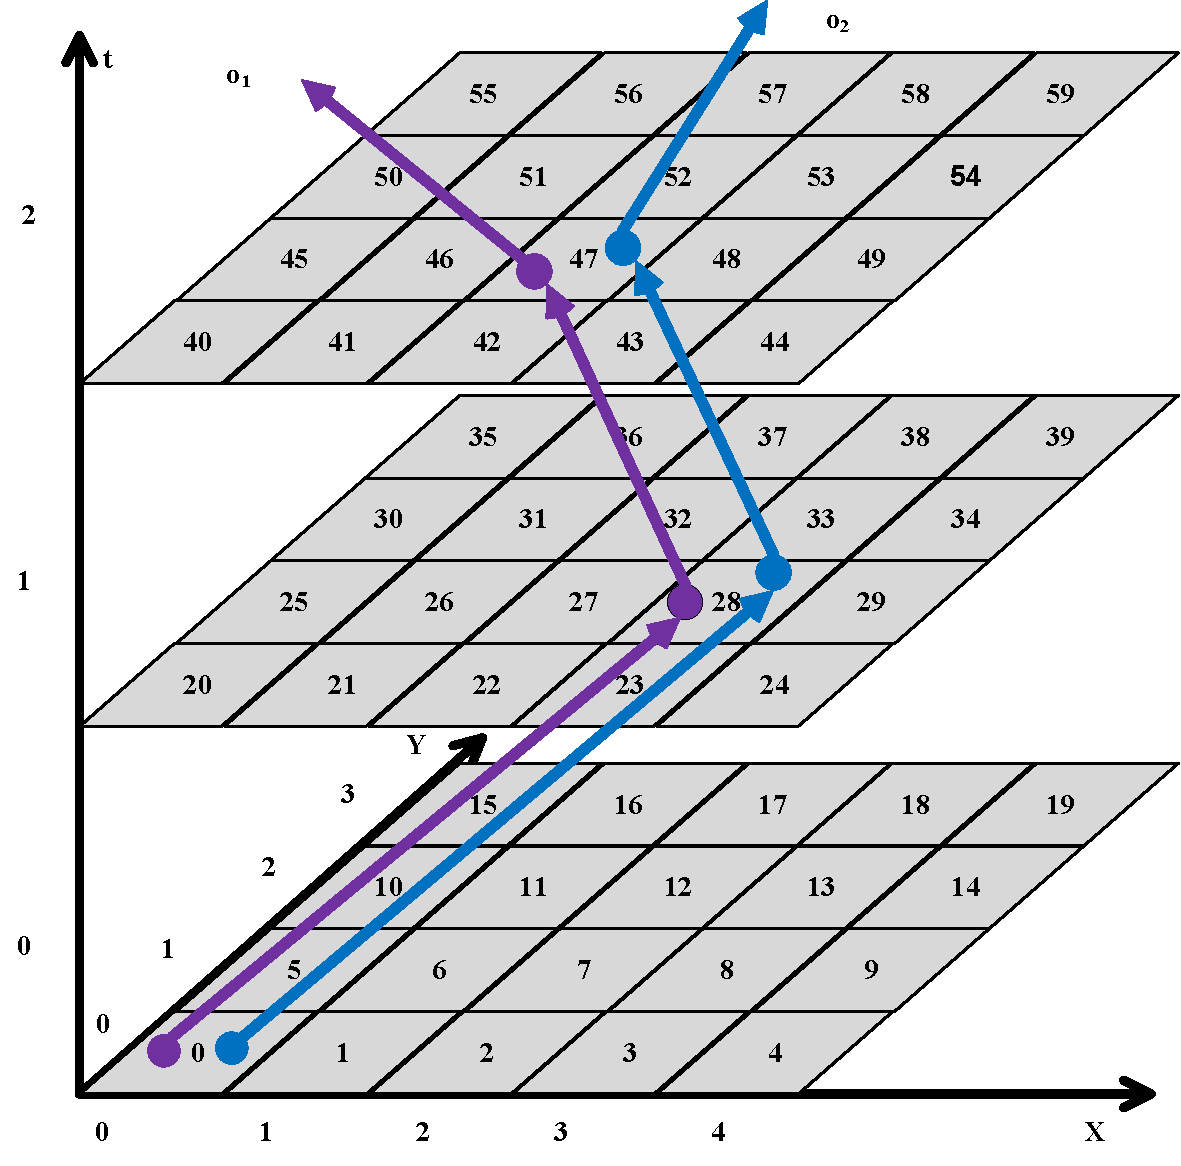
\includegraphics[width=1\textwidth]{fig/section4/picture.pdf}
	\caption{轨迹网格编号及网格编号序列示例}
	\label{cm_fig1:cell_partition}
\end{figure}

\subsubsection{近似协同行为对搜索}

基于轨迹网格编号序列，通过统计两个轨迹之间的公共网格编号数量来近似计算其协同行为持续时间。对于两个轨迹网格编号序列 $O(\tau_i)$ 和 $O(\tau_j)$，若其公共网格编号数 $|O(\tau_i)\cap O(\tau_j)|$ 不小于阈值 $k$，则将 $\langle \tau_i,\tau_j\rangle$ 记录为一个近似协同行为对。该过程对所有轨迹对执行一次，当全部轨迹网格编号序列均被评估完成后终止。

\subsection{社区感知聚类}

对于轨迹集合 $\mathcal{T}=\{\tau_1,\tau_2,\ldots,\tau_{|\mathcal{T}|}\}$，通过第一阶段近似协同行为对搜索后可获得轨迹网格编号序列集合
$O(\mathcal{T})=\{O(\tau_1),O(\tau_2),\ldots,O(\tau_{|\mathcal{T}|})\}$,
以及一组近似协同行为对。在第二阶段中，目标是发现所有满足以下条件的子集 $\mathcal{T}'\subseteq \mathcal{T}$：
(1) $|\mathcal{T}'|\geq m$；
(2) 对任意 $\tau_i,\tau_j\in\mathcal{T}'$，均有 $|O(\tau_i)\cap O(\tau_j)|\geq k$，

即满足伴随群体定义的对象集合。为此，采用聚类技术以实现高效检测。现有轨迹聚类方法主要包括基于划分的聚类 \cite{DBLP:conf/icdm/PelekisKKFT09,DBLP:conf/sigmod/LeeHW07}、基于密度的聚类 \cite{DBLP:conf/dasfaa/LiLLH10,DBLP:journals/access/LiLWYLX18} 以及基于深度学习的聚类 \cite{DBLP:conf/icde/LiZCJW18,DBLP:conf/icws/Zhang0LL019,DBLP:conf/icde/YaoCZB19}。然而，这些方法通常侧重于整体轨迹相似性建模，难以刻画对象之间的显式协同行为连接关系；同时，部分基于密度的方法在大规模数据上具有较高的计算开销。因此，上述针对轨迹聚类或表示学习提出的解决方案，均无法直接应用于本文所研究的伴随群体发现问题。其根本原因在于，聚类方法关注的
是整体轨迹相似度或嵌入空间中的距离关系，而处于同一聚类中的移动对象并不
一定在具体时间段内真实地满足时空共现约束。换言之，轨迹在全局层面上的相
似性并不能保证其在局部时间区间内存在持续的联合移动行为。因此，伴随群体
发现问题仍需基于严格的时空约束建模与结构化搜索策略进行专门设计，而不能
简单依赖现有的轨迹表示学习或聚类方法。

核心思想是将协同行为关系建模为网络（图）结构，其中节点表示移动对象，边表示近似协同行为对。一个伴随群体对应于图中由至少 $m$ 个节点构成的高度结构化子图，且任意两节点之间均满足协同行为约束。受同质性假设的启发——即共享大量协同行为邻居的对象更可能属于同一群体——采用基于共享邻居结构的社区感知聚类方法进行检测。SCAN 算法 \cite{DBLP:conf/kdd/XuYFS07} 是一种典型的社区感知聚类方法，其基于顶点结构相似性与连通性进行社区划分，时间复杂度为 $O(|P|)$，其中 $|P|$ 为协同行为对的数量（即图中的边数）。因此，SCAN 能够高效地应用于伴随群体检测任务。

\begin{theorem}
CS-ACMC 算法的时间复杂度为 $O(|\mathcal{T}|^2 \times |\tau|)$，其中 $|\mathcal{T}|$ 表示轨迹数量，$|\tau|$ 表示单条轨迹的长度。
\end{theorem}

\begin{proof}
在近似协同行为对搜索阶段，需要对每一对轨迹计算其公共网格编号数。若每条轨迹的网格编号序列长度为 $|\tau|$，则通过线性扫描或哈希统计可在 $O(|\tau|)$ 时间内完成一对轨迹的公共网格编号计算。因此，该阶段的时间复杂度为
$
O(|\mathcal{T}|^2 \times |\tau|)
$。在社区感知聚类阶段，SCAN 算法的时间复杂度为 $O(|P|)$，其中 $|P|$ 为近似协同行为对数量，且 $|P|\leq |\mathcal{T}|^2$。因此，整体时间复杂度为
$
O(|\mathcal{T}|^2 \times |\tau| + |P|)=O(|\mathcal{T}|^2 \times |\tau|)
$。综上，CS-ACMC 算法的总体时间复杂度为 $O(|\mathcal{T}|^2 \times |\tau|)$。
\end{proof}

\section{实验评估}
\label{cm_sec:exp}
在本节中，首先介绍实验设定，包括所使用的数据集与运行环境；随后给出实验结果与分析。实验主要关注所提出搜索算法在运行时间方面的表现，即高效性。通过设置不同参数，如轨迹长度、位置点密度、协同行为持续时间阈值等，对比不同算法的运行时间并进行分析。

\subsection{实验设置}

\subsubsection{数据准备}
本文实验基于两个真实世界的出租车轨迹数据集：北京出租车轨迹数据集~\cite{DBLP:conf/kdd/YuanZXS11,DBLP:conf/gis/YuanZZXXSH10}\footnote{https://www.microsoft.com/en-us/research/publication/t-drive-trajectory-data-sample/}以及波尔图出租车轨迹数据集~\footnote{https://www.kaggle.com/c/pkdd-15-predict-taxi-service-trajectory-i/data}。
\paragraph{北京出租车轨迹数据集}
该数据集记录了2008年2月2日至2008年2月8日期间，北京市10357辆出租车的GPS轨迹数据。该数据集包含了约1500万条轨迹点，总距离达到900万公里，平均采样间隔约为177秒，距离约为623米。每个文件以出租车ID命名，详细记录了时间、经度和纬度信息，为城市交通分析、出租车轨迹预测、路径规划以及地理信息系统研究提供了丰富的数据支持。
\paragraph{波尔图出租车轨迹数据集}
本研究采用的波尔图出租车轨迹数据集来源于葡萄牙波尔图市的出租车调度系统。时间跨度为 19 个月，包含超过 170 万条出租车轨迹。所有车辆均通过安装在车载终端中的移动数据设备与调度中心通信，因此能够连续采集高精度 GPS 轨迹数据。该数据集具有时间跨度长、采样频率稳定、轨迹覆盖范围广等特点，能够真实反映城市尺度下出租车群体的动态出行行为，为协同行为模式挖掘与群体结构分析提供了可靠的数据基础。

\paragraph{数据预处理}

为统一实验设定，所有时间戳均被映射到 24 小时范围内。对于波尔图数据集，每条轨迹的出发时间被随机分配至 24 小时区间内，以避免时间分布偏置。所有轨迹数据在实验前均被预处理并转换为轨迹网格编号序列。生成网格编号序列及伴随群体发现所使用的默认参数设置如表 \ref{cm_tb: group settings} 所示。同时，对轨迹的经纬度范围以及轨迹长度进行了筛选与限制，以保证实验规模可控且具有代表性，具体参数同样列于表 \ref{cm_tb: group settings} 中。

\begin{table}[tb]
	\centering
	\caption{参数设定}
	\label{cm_tb: group settings}
	\begin{tabular}{|l|l|l|}
		\hline
		\bfseries & \bfseries 北京数据集  & \bfseries 波尔图数据集 \\
		\hline
		\hline
		经度范围  & \tabincell{l}{[116.250, 116.550]} &  \tabincell{l}{[-8.735, -8.156]} \\
		\hline
		维度范围  & \tabincell{l}{[39.830,  40.030]}& \tabincell{l}{[40.953, 41.307]} \\
		\hline
		轨迹长度范围  & \tabincell{l}{[20, 100]}& \tabincell{l}{[20, 100]} \\
		\hline
		\tabincell{l}{$\epsilon_s$} & \tabincell{l}{200 米} &  \tabincell{l}{200 米} \\
  \hline
		\tabincell{l}{$\epsilon_t$} & \tabincell{l}{200 秒} &  \tabincell{l}{200 秒} \\
  \hline
		$|\mathcal{T}|$ & \tabincell{l}{2K--10K / 默认 6K}& \tabincell{l}{20K--100K / 默认 20K} \\
		\hline
  $k$ & \tabincell{l}{2--6 / 默认 4}& \tabincell{l}{2--6 / 默认 4} \\
		\hline
		 $m$ & \tabincell{l}{2--6 / 默认 4}& \tabincell{l}{2--6 /默认 4} \\
   \hline
   $\mu$ & \tabincell{l}{0.42--0.50 / 默认 0.50}& \tabincell{l}{0.42--0.50 / 默认 0.50} \\
		\hline
	\end{tabular}
\end{table}
    

\subsubsection{比较算法}

\begin{table}[htbp]
    \centering
    \setlength{\tabcolsep}{8pt}% column separation
    \caption{比较算法}
    \label{cm_tab:compared_alg}
    \renewcommand{\arraystretch}{1}%row space 
    \begin{tabular}{ll}
        \hline
		\bfseries 算法标识 & \bfseries 算法描述 \\
        \hline
        ES-ECMC & 精确搜索算法\\
        CS-ACMC & 基于近似协同行为计算的社区感知搜索算法 \\ 
        \hline
    \end{tabular}
\end{table}

表\ref{cm_tab:compared_alg}列举了实验研究中的比较算法。
本文对以下两种算法进行性能比较：ES-ECMC算法，以及CS-ACMC算法。
此外，在候选对象筛选阶段引入R树索引结构 \cite{DBLP:conf/sigmod/Guttman84}，以对空间上显然不满足距离约束的对象对进行早期剪枝，从而减少无效距离计算并提升整体运行效率。

\subsubsection{评估指标}

为了评估 CS-ACMC 算法的有效性，采用 ES-ECMC 算法所发现的精确协同行为对作为基准，并使用协同行为对的平均命中率作为主要质量评估指标。具体而言，对于 ES-ECMC 算法发现的每一个精确伴随群体 $g$，若其中任意一个协同行为对 $\langle o_i,o_j\rangle$（其中 $o_i\in g, o_j\in g$）同时存在于 CS-ACMC 算法所发现的任意一个伴随群体中，则认为该协同行为对被命中，命中计数加一；否则认为未被命中。最终统计所有精确协同行为对的命中比例，作为整体命中率。该指标能够有效反映近似算法在保持协同行为结构方面的结果质量。在效率评估方面，采用平均 CPU 运行时间作为主要性能指标。需要说明的是，在默认参数设置下，ES-ECMC 算法在北京数据集上采用单线程运行时至少需要 1 天时间，因此实验中为 ES-ECMC 启用了 40 个线程以保证实验可行性；相比之下，CS-ACMC 算法仅使用单线程运行。

\subsubsection{实验环境}
所有算法均采用 Python 实现，并运行于 Ubuntu 操作系统平台。实验硬件环境为：2 颗 Intel(R) Xeon(R) Silver 4214R CPU（主频 2.40GHz）以及 128GB 内存。除非特别说明，所有实验结果均为在 20 组不同测试轨迹输入下重复实验所得的平均值，以减少偶然因素对结果的影响。

\subsection{实验结果与分析}

\subsubsection{轨迹数量的影响}

首先，在默认参数设置下，研究轨迹数量变化对算法性能的影响。具体而言，在波尔图数据集中，轨迹数量从 20{,}000 增加至 100{,}000；在北京数据集中，轨迹数量从 2{,}000 增加至 10{,}000。之所以采用该设置，是因为北京数据集的轨迹空间分布更加密集、采样间隔更小，因此任意两条轨迹更容易满足距离约束并形成协同行为对，从而带来更高的计算压力。从命中率结果来看，波尔图数据集上的命中率随轨迹数量增加呈现明显上升趋势（见图~\ref{cm_fig:波尔图数据集-ratios-num}）。当轨迹数量由 20K 增加至 100K 时，命中率由约 0.70 提升至接近 0.88。这一现象说明，在轨迹规模较小时，近似方法可能因协同行为对数量较少而遗漏部分结构；随着轨迹数量增加，对象之间的连接关系更加充分，社区结构更加清晰，基于共享邻居的聚类策略能够更准确地恢复真实伴随群体结构。相比之下，北京数据集上的命中率始终稳定在 0.91--0.93 之间（见图~\ref{cm_fig:北京数据集-ratios-num}），整体波动较小。这是因为北京数据集本身轨迹密度较高，在较小规模下已能形成相对稳定的协同行为图结构，因此随着规模增加，近似算法的结果质量提升空间有限，但整体保持较高水平。

\begin{figure}[htbp]
    \centering
    \subfloat[]{
        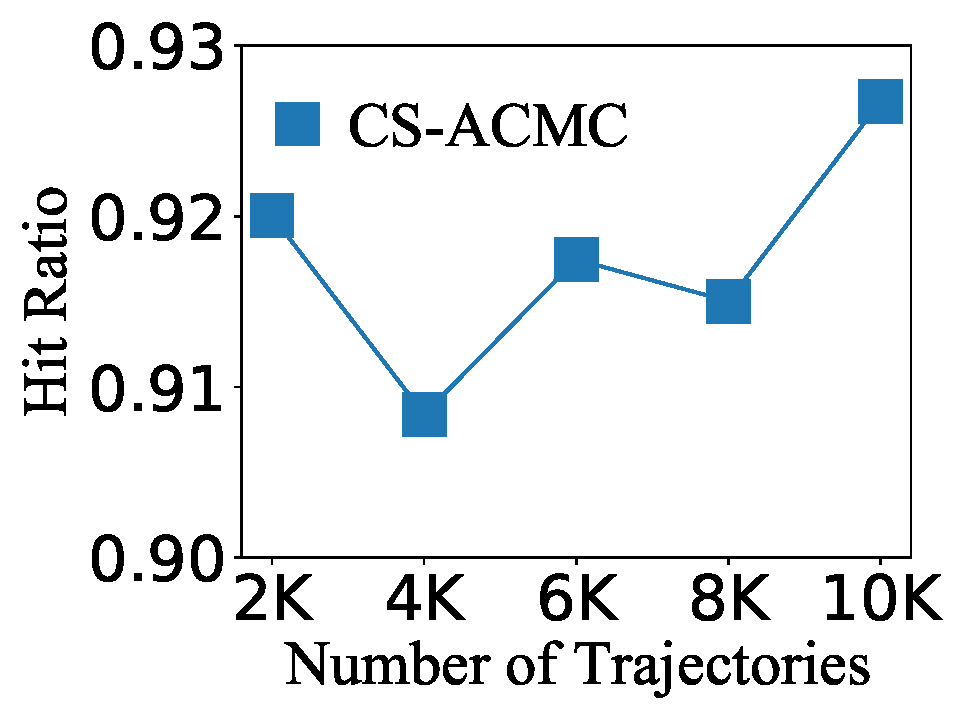
\includegraphics[width=0.4\textwidth]{fig/section4/BJ-hitratio-num.pdf}
        \label{cm_fig:北京数据集-ratios-num}
    }
    \hfill
    \subfloat[]{
        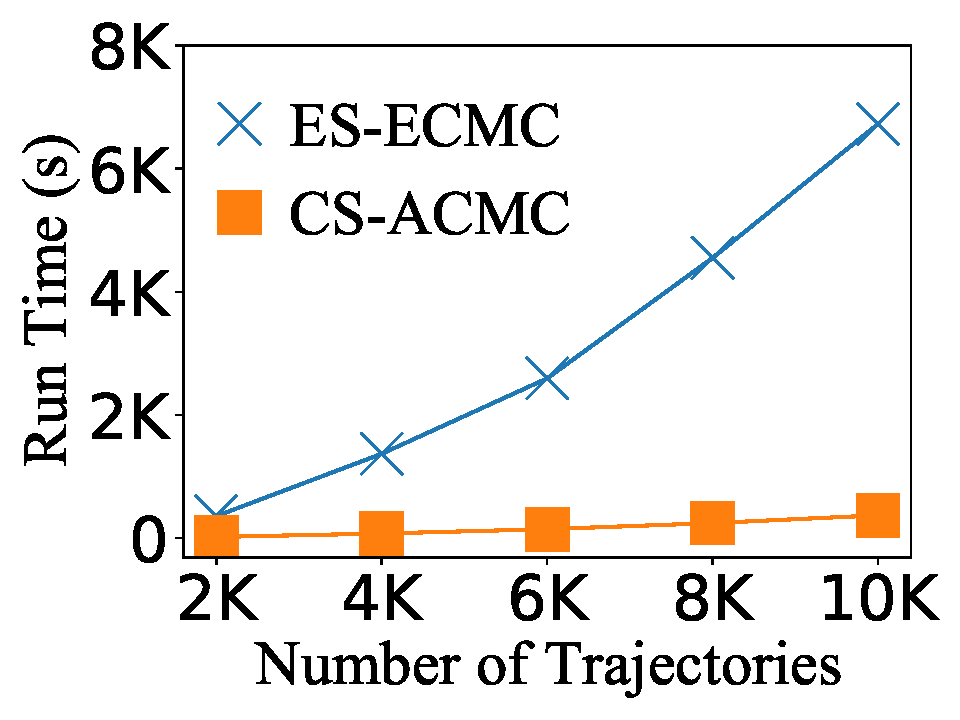
\includegraphics[width=0.4\textwidth]{fig/section4/BJ-time-num.pdf}
        \label{cm_fig:北京数据集-time-num}
    }
    \\
    \subfloat[]{
        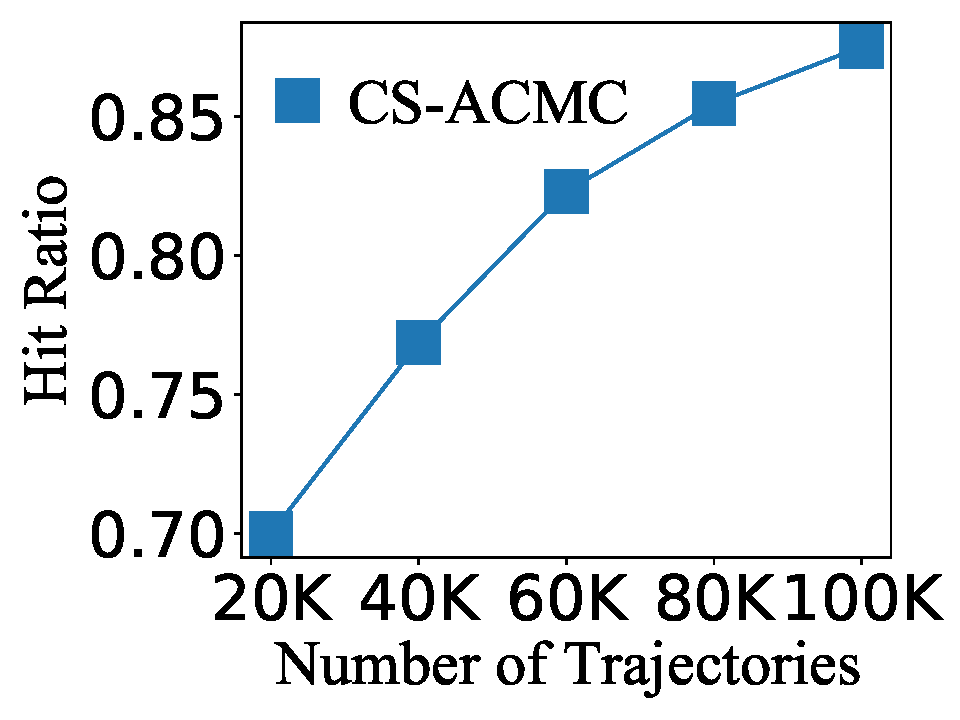
\includegraphics[width=0.4\textwidth]{fig/section4/PT-hitratio-num.pdf}
        \label{cm_fig:波尔图数据集-ratios-num}
    }
    \hfill
    \subfloat[]{
        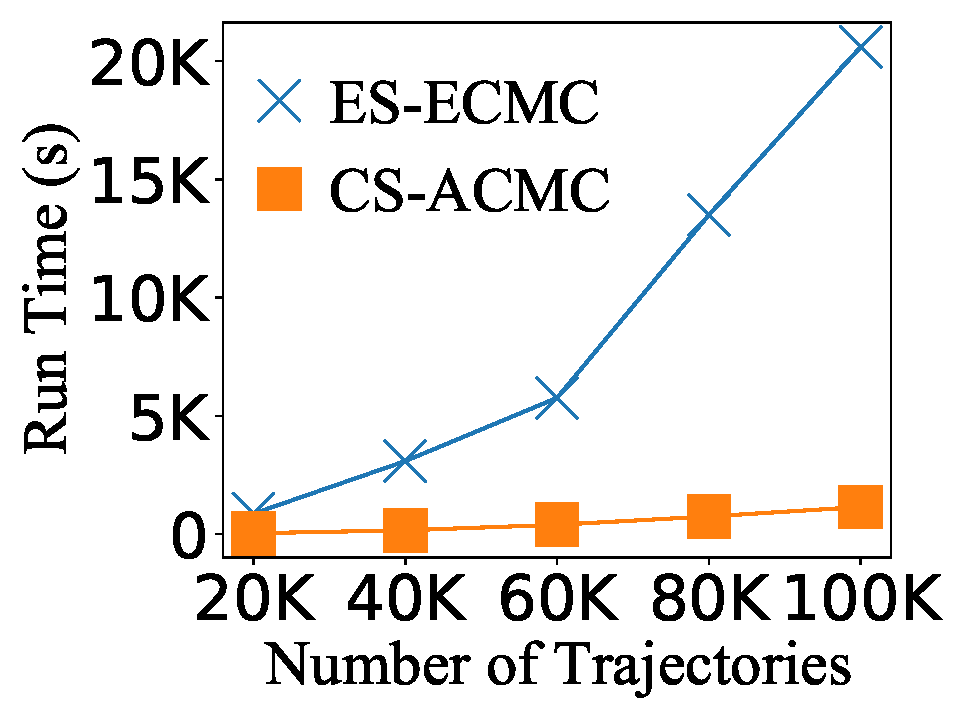
\includegraphics[width=0.4\textwidth]{fig/section4/PT-time-num.pdf}
        \label{cm_fig:波尔图数据集-time-num}
    }
    \caption{轨迹数量的影响。 \subref{cm_fig:北京数据集-ratios-num} 北京数据集上的命中率 \subref{cm_fig:北京数据集-time-num} 北京数据集上的运行时间 \subref{cm_fig:波尔图数据集-ratios-num} 波尔图数据集上的命中率 \subref{cm_fig:波尔图数据集-time-num} 波尔图数据集上的运行时间}
	\label{cm_fig:trjNum}
\end{figure}


在算法运行效率方面，两种算法的运行时间均随轨迹数量增加而增长，但增长趋势存在显著差异。ES-ECMC 的运行时间随规模增加呈现近似二次增长趋势；而 CS-ACMC 的增长速度明显更缓（见图~\ref{cm_fig:北京数据集-time-num} 和图~\ref{cm_fig:波尔图数据集-time-num}）。即便 ES-ECMC 在实验中采用了 40 线程并行计算，当轨迹数量达到 10{,}000（北京）和 100{,}000（波尔图数据集）时，其运行时间仍分别超过 8{,}000 秒和 20{,}000 秒；相比之下，CS-ACMC 在单线程条件下的运行时间始终控制在千秒以内。值得注意的是，波尔图数据集中捕获的协同行为对数量明显多于北京数据集，导致图结构更加稠密，从而增加了精确算法的计算负担。这也进一步放大了两种方法在大规模场景下的性能差距。综上所述，随着轨迹数量的增加，CS-ACMC 在保证较高命中率（尤其在大规模数据上不断提升）的同时，始终保持至少一个数量级的时间优势。这表明该方法在大规模轨迹数据分析场景下具有良好的可扩展性和实际应用价值。


\subsubsection{协同行为持续时间阈值的影响}
\begin{figure}
    \centering
    \subfloat[]{ 
        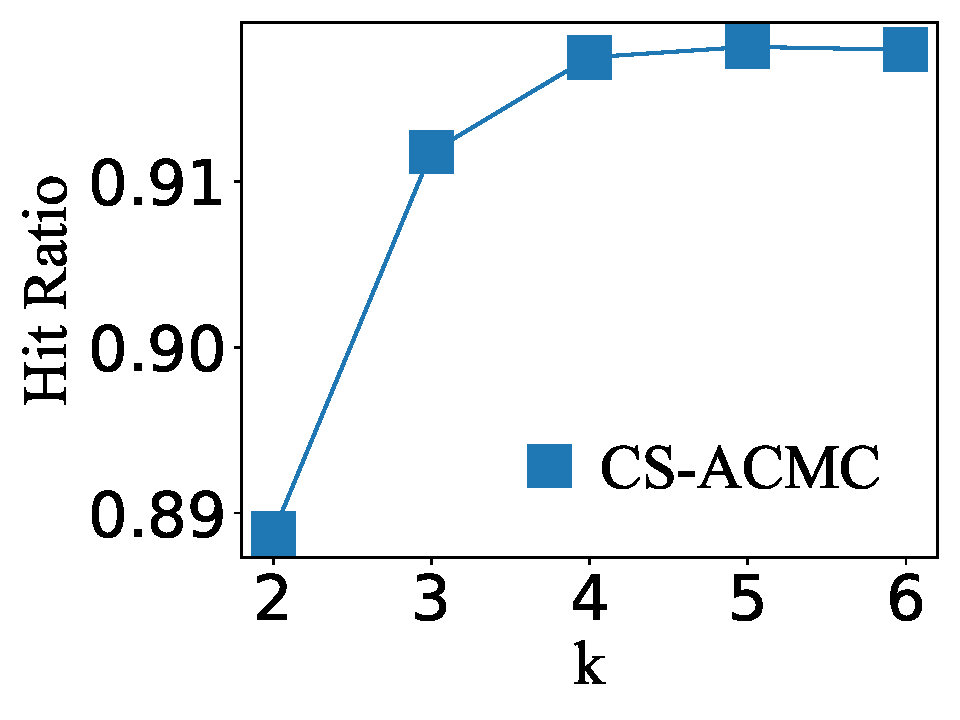
\includegraphics[width=0.4\textwidth]{fig/section4/BJ-hitratio-k.pdf}
        \label{cm_fig:北京数据集-ratios-k}
    }
    \hfill
    \subfloat[]{
        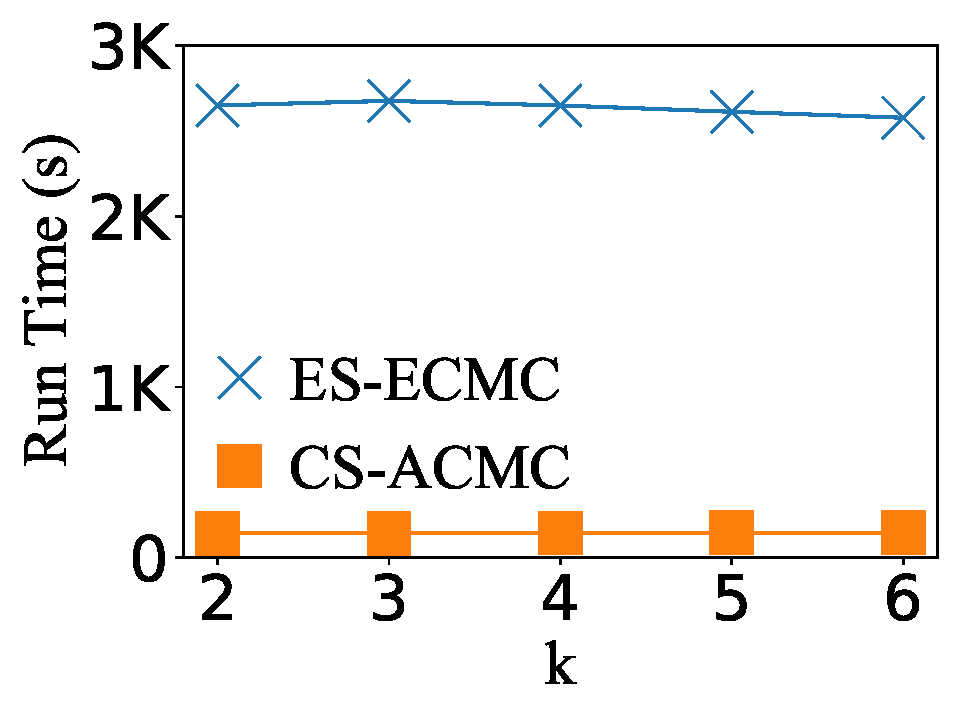
\includegraphics[width=0.4\textwidth]{fig/section4/BJ-time-k.pdf}
        \label{cm_fig:北京数据集-time-k}
    }
    \\
    \subfloat[]{
        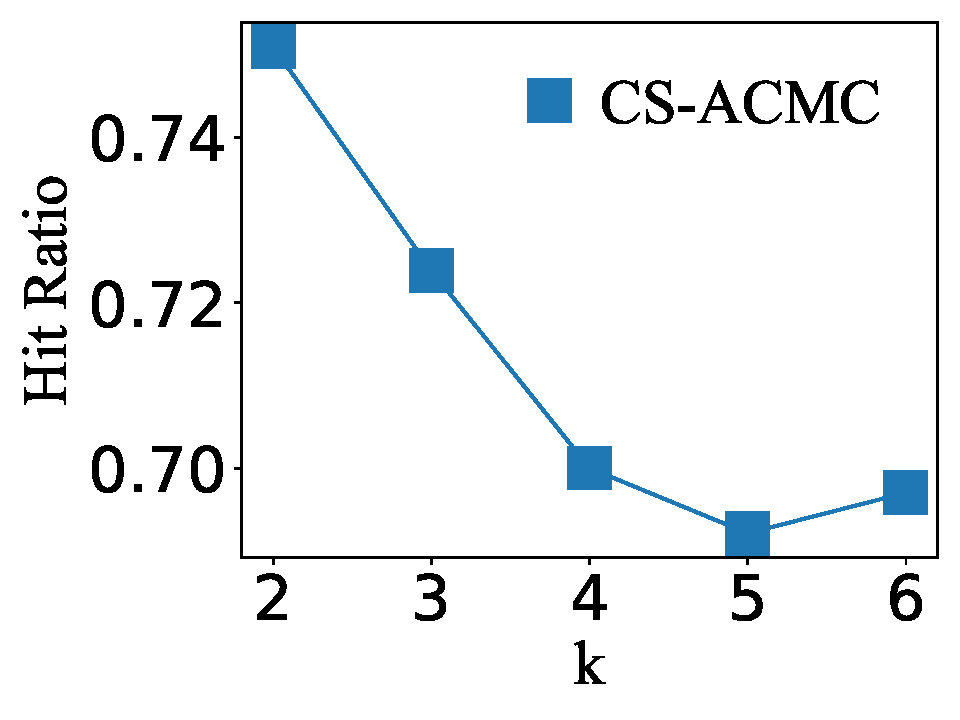
\includegraphics[width=0.4\textwidth]{fig/section4/PT-hitratio-k.pdf}
        \label{cm_fig:波尔图数据集-ratios-k}
    }
    \hfill
    \subfloat[]{
        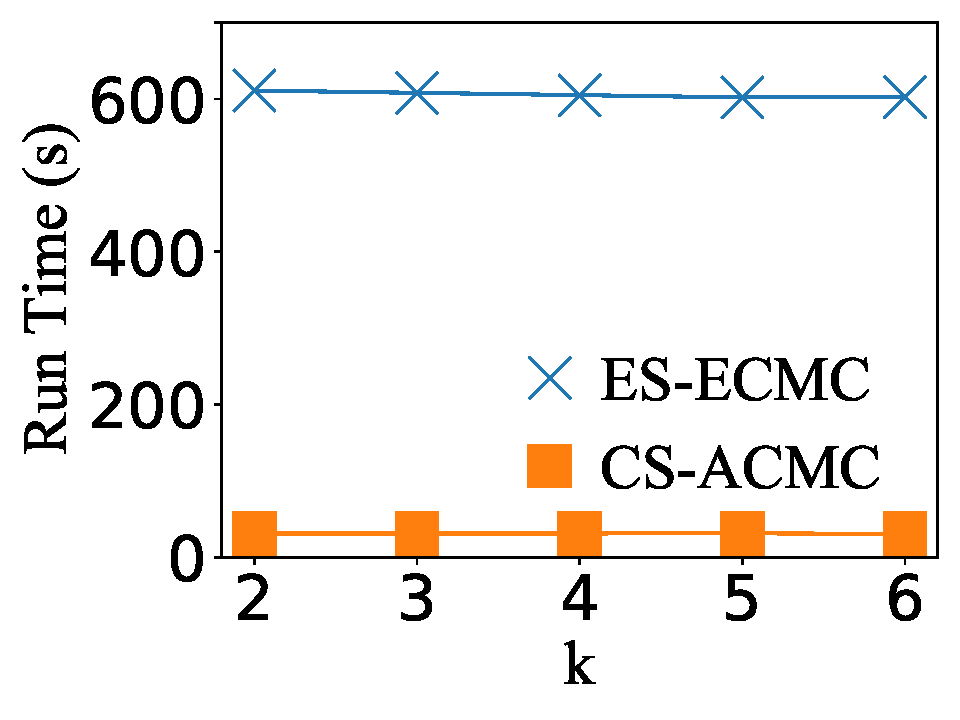
\includegraphics[width=0.4\textwidth]{fig/section4/PT-time-k.pdf}
        \label{cm_fig:波尔图数据集-time-k}
    }
    \caption{协同行为持续时间阈值的影响。\subref{cm_fig:北京数据集-ratios-k} 北京数据集上的命中率 \subref{cm_fig:北京数据集-time-k} 北京数据集上的运行时间 \subref{cm_fig:波尔图数据集-ratios-k} 波尔图数据集上的命中率 \subref{cm_fig:波尔图数据集-time-k} 波尔图数据集上的运行时间}
\label{cm_fig:k}
\end{figure}

图 \ref{cm_fig:k} 展示了当协同行为持续时间阈值 $k$ 从 2 增加到 6 时两种算法的性能变化趋势。
从命中率角度来看，北京数据集上的命中率随 $k$ 增大呈现缓慢上升趋势（见图~\ref{cm_fig:北京数据集-ratios-k}）。当 $k=2$ 时命中率约为 0.89，随后逐步提升并稳定在 0.91 以上。这表明在北京这种高密度轨迹环境下，提高持续时间阈值能够有效过滤掉短暂、偶然的协同行为，使近似方法更聚焦于结构稳定的协同行为对，从而提升结果质量。相比之下，波尔图数据集上的命中率随着 $k$ 的增大整体呈下降趋势（见图~\ref{cm_fig:波尔图数据集-ratios-k}），从约 0.75 下降至 0.69 左右。这是因为波尔图数据集采样频率更高、时间跨度更长，较大的 $k$ 会显著减少满足条件的协同行为对数量，使得图结构变得稀疏，进而影响基于共享邻居的社区识别效果。因此，近似方法在较大 $k$ 下更容易遗漏部分真实协同行为结构。

在运行时间方面，如图~\ref{cm_fig:北京数据集-time-k} 和图~\ref{cm_fig:波尔图数据集-time-k}，两种算法均未随着 $k$ 的增大而出现明显下降趋势。尽管理论上更大的 $k$ 会减少协同行为对及伴随群体数量，从而降低后续聚类成本，但实验结果表明，总体运行时间基本保持稳定。其主要原因在于，算法的核心计算开销集中在协同行为对的枚举或近似计算阶段，而该阶段需要对所有轨迹对进行比较，其复杂度与 $k$ 无关；从协同行为对中生成伴随群体的代价相对较低，因此 $k$ 的变化对总时间影响有限。同时可以观察到，在所有 $k$ 取值下，CS-ACMC 的运行时间始终显著低于 ES-ECMC。即使在较小 $k$（的情况下，CS-ACMC 仍保持明显的效率优势，进一步验证了近似计算策略在降低计算成本方面的有效性。

\subsubsection{群体规模阈值的影响}

图 \ref{cm_fig:m} 展示了当群体规模阈值 $m$ 从 2 变化到 6 时两种算法性能的变化趋势。直觉上，随着 $m$ 的增大，满足条件的伴随群体数量逐渐减少，因为只有结构更加紧密、连接更加稳定的对象集合才能满足更严格的规模约束。这一变化对结果质量与运行时间均产生一定影响。如图~\ref{cm_fig:北京数据集-ratios-m}，北京数据集上的命中率随着 $m$ 的增加呈显著上升趋势。当 $m=2$ 时命中率约为 0.71，而当 $m=5$ 或 $6$ 时可提升至 0.93 左右。这说明在高密度轨迹环境下，小规模群体中包含较多边界性或弱连接结构，近似方法可能存在一定偏差；而当 $m$ 增大后，仅保留结构更加紧密的核心群体，使得近似方法与精确方法在识别结果上更加一致，从而显著提升命中率。相比之下，波尔图数据集上的命中率随着 $m$ 的增加呈下降趋势，从约 0.88 下降至 0.59 左右。这主要是由于波尔图数据集数据的空间分布更为分散、轨迹时间跨度更长。当 $m$ 较大时，满足条件的群体数量显著减少，图结构趋于稀疏，近似协同行为对可能无法完整保留所有真实连接关系，导致部分精确群体未被成功恢复，从而降低命中率。

在效率方面（见图~\ref{cm_fig:北京数据集-time-m} 和图~\ref{cm_fig:波尔图数据集-time-m}），群体规模阈值 $m$ 的变化对总体运行时间影响较小。两种算法的运行时间曲线基本保持平稳，仅在个别取值处存在轻微波动。这进一步验证了前文分析：算法的主要时间开销集中在协同行为对的构建或近似计算阶段，而最终伴随群体的筛选与过滤成本相对较低，因此 $m$ 的变化不会显著改变总体时间复杂度。
同时可以观察到，在所有 $m$ 取值下，CS-ACMC 的运行时间始终远低于 ES-ECMC。即使在波尔图数据集中，当 $m=6$ 时 ES-ECMC 的运行时间超过 8{,}000 秒，而 CS-ACMC 仍保持在数百秒以内，体现出明显的规模优势。
综上所述，在不同 $m$ 参数设置下，CS-ACMC 在保持较高命中率（尤其在高密度数据集上）的同时，显著降低了运行时间，表现出良好的稳定性与参数鲁棒性。这表明该方法能够适应不同规模约束条件，在多种实际应用场景中具有较强的实用价值。


\begin{figure}[htbp]
    \centering
    \subfloat[]{
        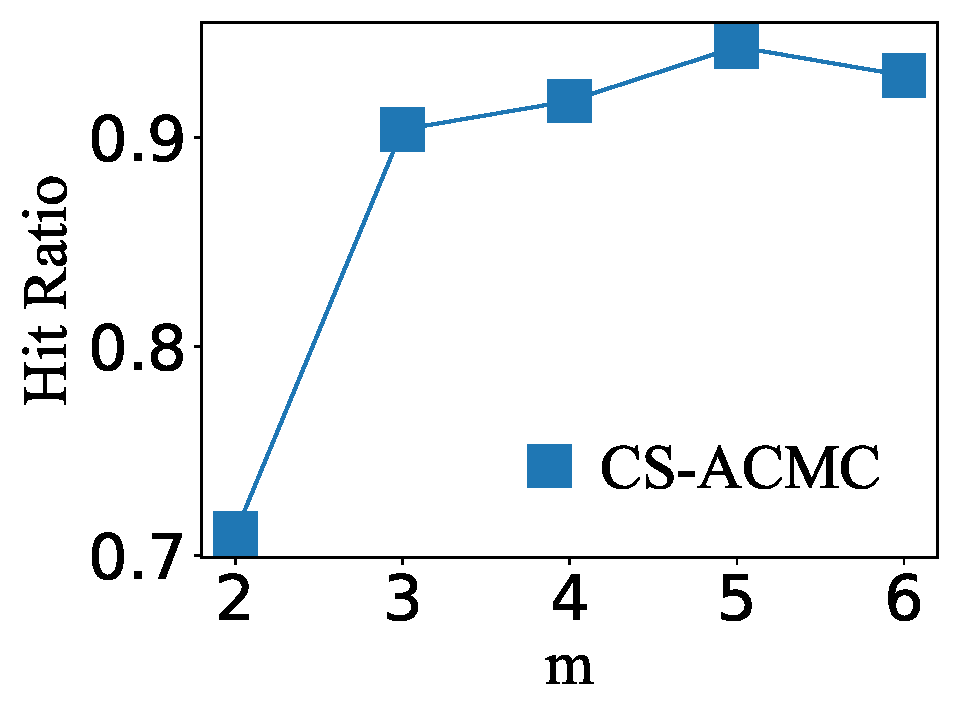
\includegraphics[width=0.4\textwidth]{fig/section4/BJ-hitratio-m.pdf}
        \label{cm_fig:北京数据集-ratios-m}
    }
    \hfill
    \subfloat[]{
        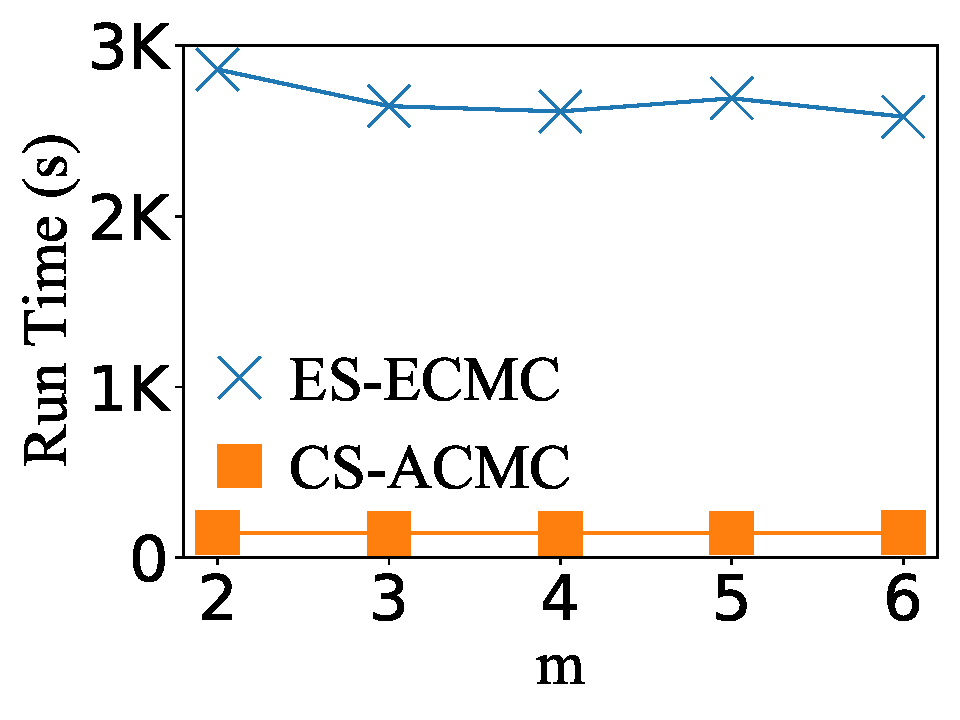
\includegraphics[width=0.4\textwidth]{fig/section4/BJ-time-m.pdf}
        \label{cm_fig:北京数据集-time-m}
    }
    \\
    \subfloat[]{
        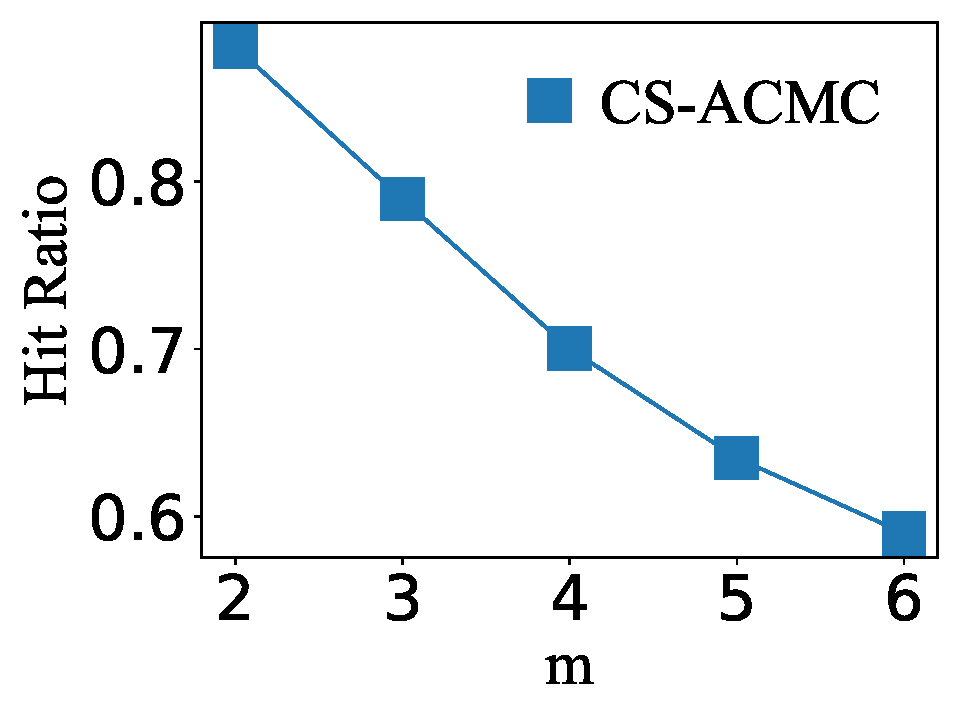
\includegraphics[width=0.4\textwidth]{fig/section4/PT-hitratio-m.pdf}
        \label{cm_fig:波尔图数据集-ratios-m}
    }
    \hfill
    \subfloat[]{
        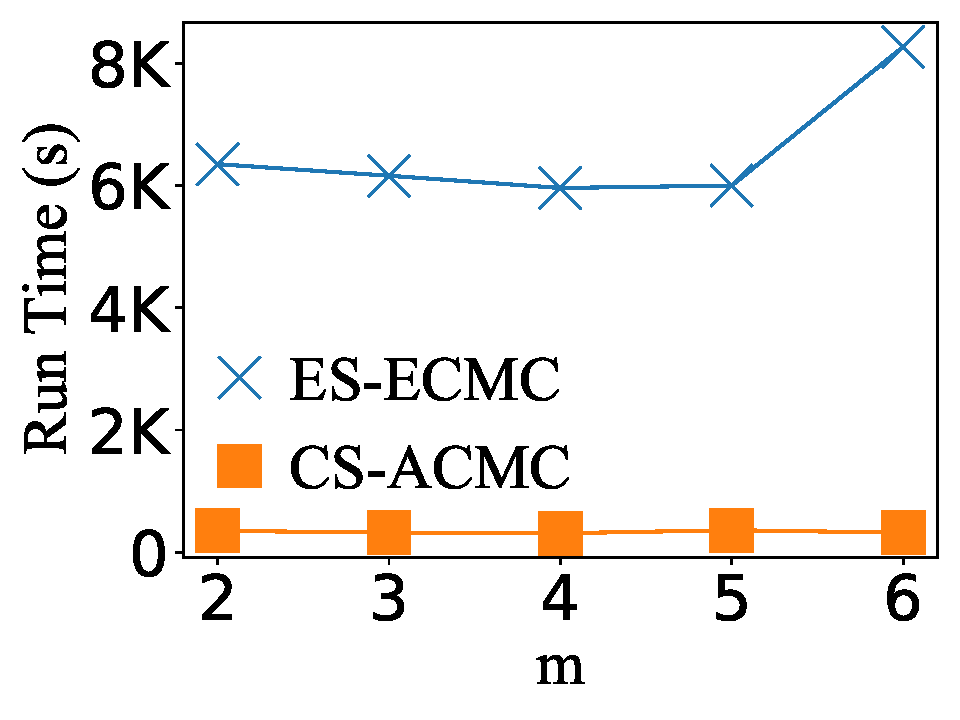
\includegraphics[width=0.4\textwidth]{fig/section4/PT-time-m.pdf}
        \label{cm_fig:波尔图数据集-time-m}
    }
    \caption{群体规模阈值的影响。\subref{cm_fig:北京数据集-ratios-m} 北京数据集上的命中率 \subref{cm_fig:北京数据集-time-m} 北京数据集上的运行时间 \subref{cm_fig:波尔图数据集-ratios-m} 波尔图数据集上的命中率 \subref{cm_fig:波尔图数据集-time-m} 波尔图数据集上的运行时间}
    \label{cm_fig:m}
\end{figure}


\subsubsection{聚类参数的影响}
\begin{figure}[htbp]
    \centering
    \subfloat[]{
        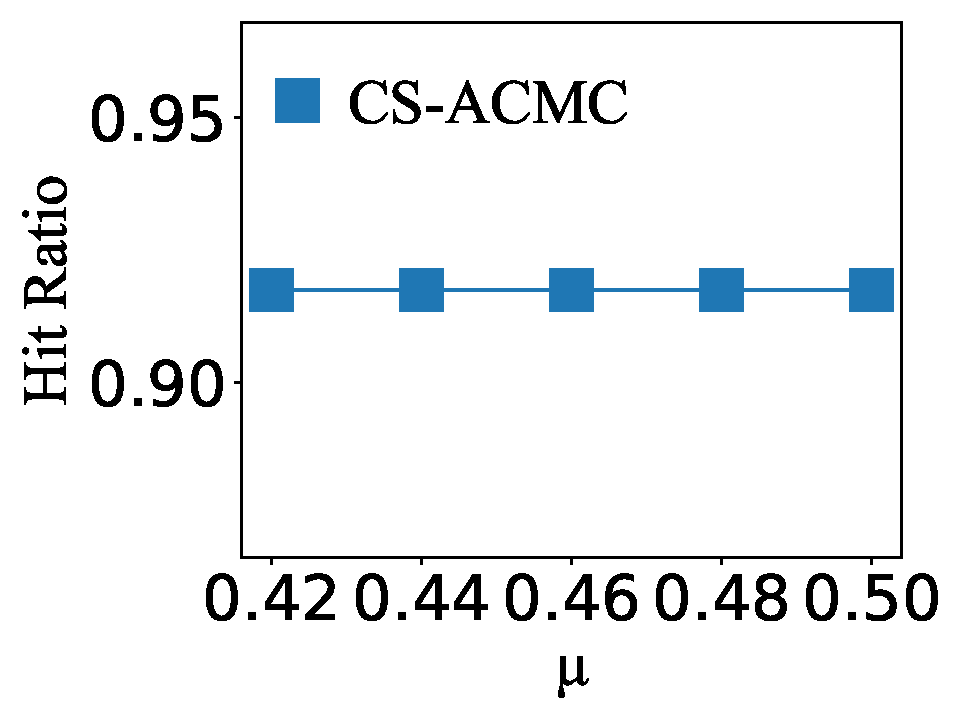
\includegraphics[width=0.4\textwidth]{fig/section4/BJ-hitratio-ep.pdf}
        \label{cm_fig:北京数据集-ratios-ep}
    }
    \hfill
    \subfloat[]{
        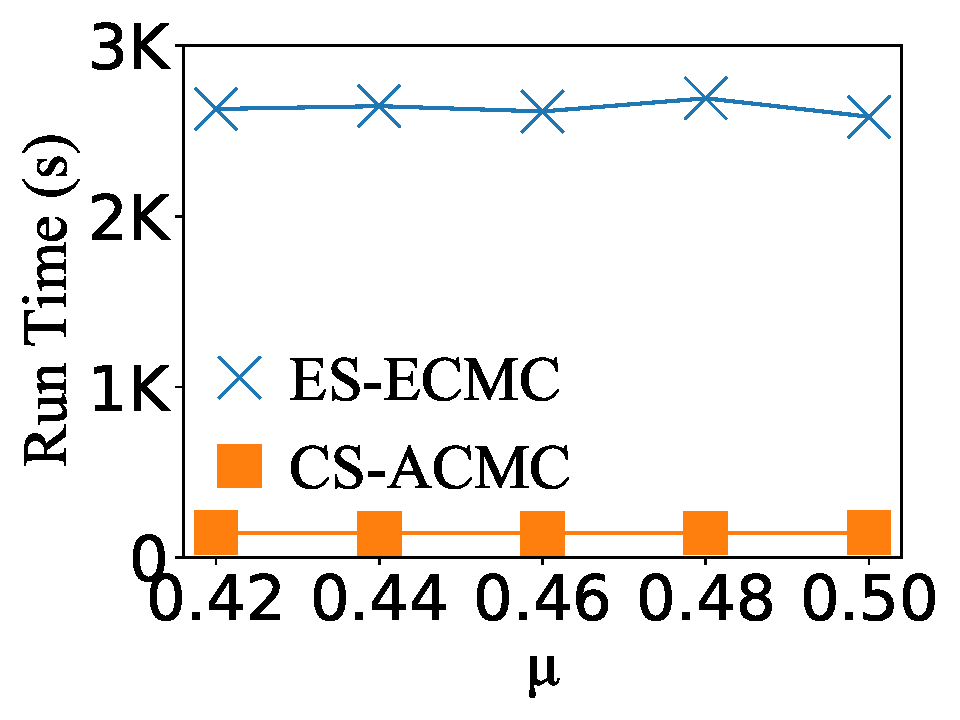
\includegraphics[width=0.4\textwidth]{fig/section4/BJ-time-ep.pdf}
        \label{cm_fig:北京数据集-time-ep}
    }

    \subfloat[]{
        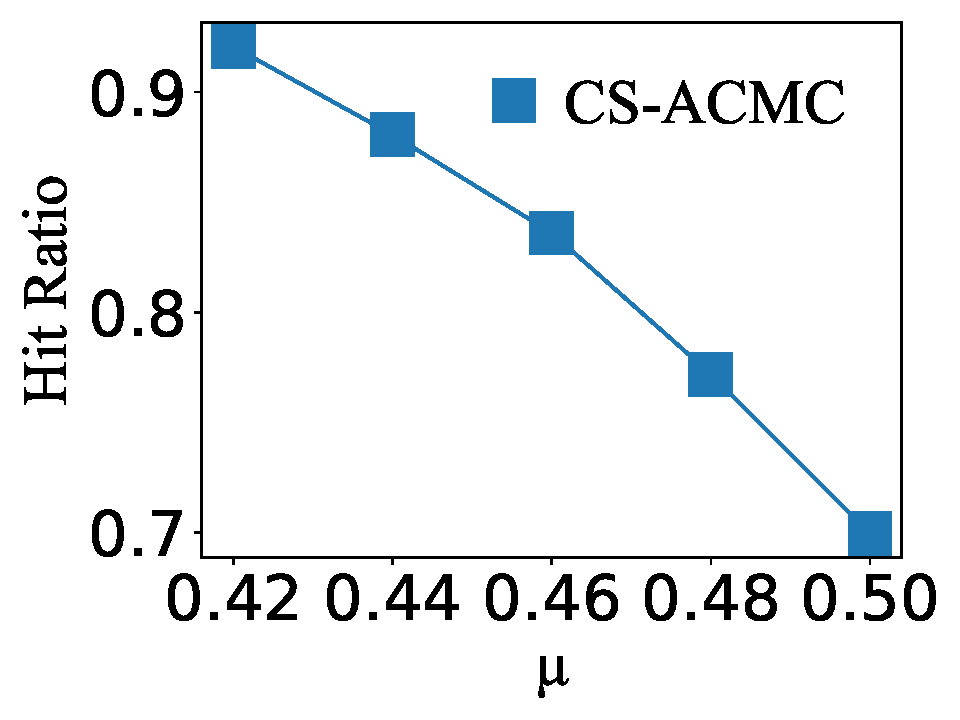
\includegraphics[width=0.4\textwidth]{fig/section4/PT-hitratio-ep.pdf}
        \label{cm_fig:波尔图数据集-ratios-ep}
    }
    \hfill
    \subfloat[]{
        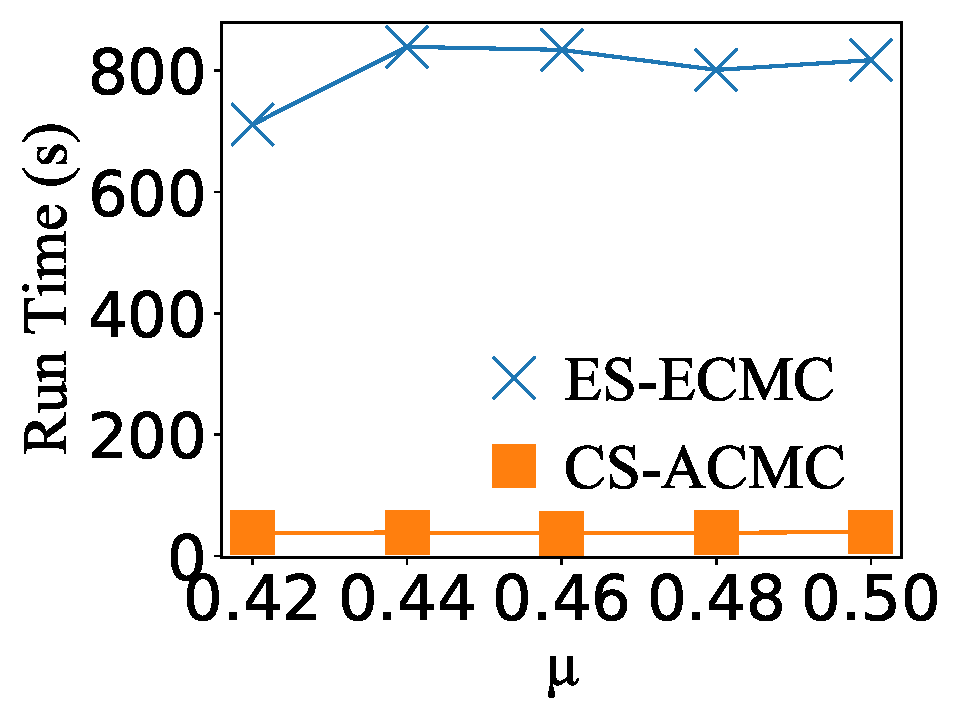
\includegraphics[width=0.4\textwidth]{fig/section4/PT-time-ep.pdf}
        \label{cm_fig:波尔图数据集-time-ep}
    }
    \caption{SCAN聚类结构相似度参数的影响。\subref{cm_fig:北京数据集-ratios-ep} 北京数据集上的命中率 \subref{cm_fig:北京数据集-time-ep} 北京数据集上的运行时间 \subref{cm_fig:波尔图数据集-ratios-ep} 波尔图数据集上的命中率 \subref{cm_fig:波尔图数据集-time-ep} 波尔图数据集上的运行时间}
    \label{cm_fig:ep}
\end{figure}


图 \ref{cm_fig:ep} 展示了当结构相似度阈值 $\mu$ 从 0.42 增加到 0.50 时算法在两个数据集上的命中率与运行时间变化情况。结构相似度阈值用于控制对象之间是否建立连接：$\mu$ 越小，两个对象越容易满足相似性条件，从而在协同行为图中形成更多边；$\mu$ 越大，则连接关系更加严格，图结构趋于稀疏。

从命中率变化趋势来看，在波尔图数据集中（见图~\ref{cm_fig:波尔图数据集-ratios-ep}），随着 $\mu$ 的增大，命中率呈现明显下降趋势。当 $\mu=0.42$ 时取得最佳效果，而当 $\mu=0.50$ 时命中率下降至约 0.70。这表明在空间分布较为分散的数据环境下，适当放宽结构相似度约束有助于保留潜在的真实连接关系，而过高的阈值会导致部分真实协同关系被过滤，进而影响整体命中率。相比之下，北京数据集上的命中率始终稳定在 0.91 以上，且随 $\mu$ 的变化波动较小（见图~\ref{cm_fig:北京数据集-ratios-ep}）。这一现象主要归因于北京数据集更高的轨迹采样密度和更强的空间聚集性。在高密度环境中，即使提高相似度阈值，真实协同行为之间仍能保持较高的结构一致性，因此算法结果对 $\mu$ 的敏感度较低，表现出更强的稳定性。

在效率方面（见图~\ref{cm_fig:北京数据集-time-ep} 和图~\ref{cm_fig:波尔图数据集-time-ep}），两种算法的运行时间均未随 $\mu$ 的变化出现显著波动，说明结构相似度阈值主要影响图的连接密度，而对整体计算流程的复杂度影响有限。然而，即便 ES-ECMC 采用多线程实现，其运行时间仍显著高于 CS-ACMC，在两个数据集上均至少相差一个数量级。这表明本文提出的近似协同行为构建策略在降低候选连接数量的同时，有效控制了计算开销。

\section{本章小结}
\label{cm_sec:conclusion}

针对传统协同行为模式定义过于严格、难以适应真实轨迹数据中噪声与不规则性的不足，提出了一种放宽的协同行为模式定义，在保证语义合理性的同时，提高了模型对实际数据的适应能力。

从数据处理模式的角度来看，现有方法可大致分为静态处理与流式处理两类。一些方法（如~\cite{DBLP:conf/icde/ZhengZYS13,DBLP:journals/tkde/ZhengZYSZ14,DBLP:conf/sigmod/FangGPCMJ20}）能够处理轨迹数据流，支持持续更新与在线检测；而另一些方法则主要面向离线或静态轨迹数据（如~\cite{DBLP:conf/gis/VieiraBT09,DBLP:journals/pvldb/JeungYZJS08,DBLP:journals/pvldb/LiDHK10}）。与本文最为相关的工作之一是 Chen 等人~\cite{DBLP:journals/pvldb/ChenGFMJG19} 提出的实时联合移动模式挖掘方法。该方法定义了一种更为通用的联合移动模式，并通过 $L$-连续性与 $G$-连通性刻画轨迹之间的时间连续性与结构连通性。然而，由于问题定义存在本质差异，该方法无法直接应用于本文场景：一方面，本文不要求时间上的严格连续性或连通性；另一方面，也不要求对象在每个时间点均属于同一聚类结构；此外，当一个对象能够参与多个群体时，本文采用“成员规模最大优先”的归属策略，以保证结果的确定性与可解释性。

围绕上述问题，分别设计了精确算法与近似算法。精确算法通过完整枚举与严格验证协同行为对，能够获得理论上的最优结果，但在大规模数据场景下面临较高的时间复杂度。为此，进一步提出了基于结构剪枝与候选压缩策略的近似算法，通过构建紧凑的协同行为图结构，有效减少冗余计算与无效候选，从而在保证较高命中率的前提下显著降低运行开销。两种算法在设计思路上相互补充：前者保证结果精确性，后者强调规模可扩展性，共同构成了完整的解决方案体系。

在实验评估方面，基于北京与波尔图数据集两个真实世界轨迹数据集，从轨迹数量、协同行为持续时间阈值 $k$、群体规模阈值 $m$ 以及结构相似度阈值 $\mu$ 等多个维度进行了系统分析。实验结果表明：（1）在不同数据规模下，CS-ACMC 均表现出良好的可扩展性，其运行时间相比 ES-ECMC 至少降低一个数量级；（2）在高密度数据集上，近似算法能够保持稳定且较高的命中率，体现出较强的鲁棒性；（3）参数变化对算法运行时间影响有限，说明主要计算开销集中在协同行为对构建阶段；（4）在不同数据分布特性下，结构相似度与群体规模参数对命中率的影响具有一定差异，进一步验证了方法在多场景下的适应能力。

从应用角度来看，本章研究成果对于交通管理与城市计算具有重要意义。通过对潜在协同行为群体的提前识别，可以辅助分析车队行驶、异常聚集、隐性组织化出行等行为模式，为拥堵预测、路径规划优化以及公共安全监测提供数据支持。同时，所提出的近似建模与剪枝策略也可推广至其他大规模时空模式挖掘任务，具有较强的通用性。


	% \chapter{面向疾病传播控制：大规模移动对象上的连续暴露发现}

\section{引言}
传染性疾病长期以来一直被视为重大的公共卫生问题。密切接触发现（close contact discovery）在防止疫情传播方面发挥着不可或缺的作用。在此背景下，我们研究\textbf{连续暴露搜索问题}：给定一组移动对象和一组移动查询对象，在一段时间内持续地发现所有直接或间接暴露于至少一个查询对象的对象。

该问题面向多种应用场景，包括但不限于疾病防控、疫情预警、信息传播分析以及共移动模式挖掘。

为了解决该问题，我们设计了一种带有优化策略的精确群组处理算法。此外，我们还提出了一种近似算法，在不产生漏检（false dismissal）的前提下显著提升了计算效率。大量实验结果验证了所提出算法在有效性和效率方面的优势。
\subsection{研究背景与意义}
随着位置追踪设备（如车载导航系统和智能手机）以及 GPS 赋能服务（如 Google Maps）的持续普及，轨迹数据的规模正在迅速增长。在多种轨迹查询任务中~\cite{DBLP:conf/icde/ChenSJ0K20,DBLP:journals/vldb/ShangCWJZK18,DBLP:conf/ijcai/ChenSFK21,DBLP:journals/tkde/ShangCZJWK19}，接触搜索与接触追踪问题近年来受到了广泛关注~\cite{DBLP:journals/pvldb/Xu0B20,DBLP:conf/dasfaa/ChaoHLZ021,react}。一般而言，当两个移动对象在一段时间内保持较近的空间距离并相互影响时，即构成一次密切接触。对密切接触进行高效、准确的发现，在诸多实际场景中具有重要意义，包括但不限于疾病防控、疫情预警、信息传播分析以及共移动模式挖掘。在疫情期间，实时发现密切接触对象有助于限制人群传播并评估个体感染风险。

现有研究主要聚焦于针对单个查询对象（或查询轨迹）的接触追踪问题，通常基于查询对象与数据对象之间的空间邻近性进行处理（如~\cite{DBLP:conf/sigmod/FaloutsosRM94,DBLP:journals/pvldb/AssentWKKS09}），也有部分研究基于轨迹片段之间的相似性计算开展分析（如~\cite{DBLP:conf/icde/RongLSWLD17,DBLP:journals/pvldb/XieLP17}）。然而，在疾病暴发期间，大规模个体可能在短时间内被感染，因此，基于轨迹对海量移动对象进行连续接触搜索显得尤为重要。一个有效的接触搜索方法不仅需要能够同时处理大规模移动对象，还应保证对每个对象的实时检测能力。

据我们所知，现有研究通常将该问题建模为独立的查询处理问题、轨迹搜索问题~\cite{DBLP:journals/information/AlarabiBHA21,DBLP:conf/dasfaa/ChaoHLZ021}，或多查询搜索问题~\cite{DBLP:journals/corr/abs-2004-06653,DBLP:ptop}。这些方法要么仅适用于少量查询，要么假设输入为静态轨迹集合，因而在实际场景中难以有效处理大规模移动对象及大量查询。此外，这些方法也难以为每个对象持续维护实时检测结果。

\begin{figure}[t]
    \centering
    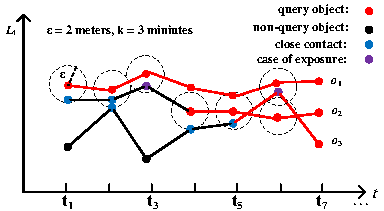
\includegraphics[width=0.8\textwidth]{fig/section5/intro.pdf}
    \caption{Example of cases of exposure}
    \label{fig:intro}
\end{figure}
\subsection{相关工作}
与我们研究的问题相似的一个方向是协同行为模式挖掘（co-movement pattern mining）。现有研究已经讨论了多种有趣的协同行为模式
\cite{DBLP:journals/pvldb/JeungYZJS08,DBLP:journals/pvldb/LiDHK10,flock,tang,DBLP:conf/icde/ZhengZYS13}。
其中，flock 模式 \cite{flock} 是最早提出的协同行为模式，用于刻画在连续 $k$ 个时间区间内共同移动的 $m$ 个移动对象组成的群体。
在相关工作中，文献 \cite{DBLP:conf/icde/ZhengZYS13} 从交通拥堵发现的角度提出了 gathering 模式。
此外，文献 \cite{tang} 以流式方式挖掘协同行为群体。
与上述研究不同的是，我们的 CES 问题不要求对群体中对象数量进行约束。
需要注意的是，在我们的定义下，群体之外的对象也可能被视为感染对象。
因此，这些研究提出的解决方案均无法直接应用于我们的问题。

为了有效防止 SARS、埃博拉以及 COVID-19 等传染病的传播，已有大量相关研究被提出
\cite{web,DBLP:journals/pvldb/Xu0B20,DBLP:journals/corr/abs-2004-06653}。
其中，文献 \cite{DBLP:journals/pvldb/Xu0B20} 首次提出了接触追踪（contact tracing）问题，
但该工作主要关注疾病传播的模拟，无法支持实时查询。
从另一个角度来看，文献 \cite{web} 提出了接触追踪查询（Contact Tracing Query, CTQ），
用于识别与查询对象存在直接或间接接触的个体。
文献 \cite{DBLP:conf/dasfaa/ChaoHLZ021} 提出了广义轨迹接触搜索（Trajectory Contact Search, TCS）查询，并设计了一种迭代算法进行求解。
另一项相关工作 \cite{DBLP:journals/information/AlarabiBHA21} 提出了一种用于追踪与患者接触的所有对象并搜索潜在感染者的技术，
但该方法基于轨迹片段，且主要面向室内应用场景。
据我们所知，现有方法均无法直接用于解决本文提出的问题，
因为它们要么针对静态轨迹数据，要么采用了不同的暴露案例定义。
\subsection{研究成果与贡献}

在此背景下，我们定义并研究了连续暴露搜索（Continuous Exposure Search，CES）问题：给定一组移动对象 $\mathcal{O}$，以及一个查询集合 $\mathcal{Q}\in\mathcal{O}$，用于表示已有的暴露病例，我们的目标是通过实时更新 $\mathcal{Q}$，持续检测新的暴露病例。在我们的设定中，新的暴露病例是指在距离阈值 $\epsilon$ 内、并且在时间阈值 $k$ 内与查询对象共同移动的对象。

如图 \ref{fig:intro} 所示的示例中，设 $o_1, o_2, o_3$ 为三个移动对象，初始查询集合为 $\mathcal{Q}=\{o_1\}$。距离阈值 $\epsilon$ 设为 2 米，接触时长阈值 $k$ 设为 3 分钟。我们使用红色、蓝色和紫色点分别表示已暴露（查询）对象的位置、密切接触对象的位置以及最新确认的暴露病例的位置。对象 $o_2$ 在连续时间段 $[t_1, t_3]$ 内与查询对象 $o_1$ 保持密切接触，因此我们将 $o_2$ 加入查询集合，即更新为 $\mathcal{Q}=\{o_1,o_2\}$，并在 $t_3$ 时刻返回更新后的 $\mathcal{Q}$ 作为实时结果。类似地，对象 $o_3$ 在时间段 $[t_4, t_6]$ 内与查询对象发生密切接触，因此在 $t_6$ 时刻将查询集合更新为 $\mathcal{Q}=\{o_1,o_2,o_3\}$。

为 CES 问题设计一种既高效又有效的解决方案并非易事。直接方法难以应对大规模移动对象，同时也无法保证实时性。为此，我们提出了一种高效的精确实时搜索算法，并引入多种优化技术。此外，我们还提出了一种近似实时搜索算法，在不产生漏检的前提下进一步提升搜索效率。本文的主要贡献总结如下：

\begin{itemize}
     \item 我们定义了一种新的 CES 问题，用于在大量移动对象中持续维护最新的暴露病例。该问题有助于监测和控制流行病的传播，例如 SARS、埃博拉和 COVID-19。
     \item 我们提出了两种算法来解决 CES 问题，分别是精确实时搜索算法 Exact Group Processing（EGP）和近似实时搜索算法 Approximate Group Processing（AGP）。同时，我们设计了分组过滤和预检查策略以提升搜索效率。
     \item 我们在两个真实数据集上进行了大量实验来评估所提方法的有效性和效率。实验结果表明，该方法能够在大规模移动对象场景下实时检测暴露病例。
\end{itemize}

\section{问题描述}
我们以一组移动对象 $\mathcal{O}=\{o_1,\ldots,o_n\}$ 以及一个查询对象集合 $\mathcal{Q}$（$\mathcal{Q}\subseteq\mathcal{O}$）作为输入。在现实场景中，例如，移动对象可以是行人，而查询对象可以是已暴露于新冠病毒的人群。我们的目标是以实时的方式检测潜在的暴露案例。接下来，我们将在本节其余部分中定义一些重要概念。

\begin{definition}[移动对象的位置流]
移动对象 $o$ 在时间 $t$ 的位置表示为 $l_t^o=([x,y],t)$，其中 $[x,y]$ 表示空间坐标，$t$ 表示时间戳。需要注意的是，$l_t^o$ 是动态更新的。我们使用 $L_t(\mathcal{O})=\{l_t^o \mid o\in \mathcal{O}\}$ 来表示所有移动对象在时间 $t$ 的位置集合。
\end{definition}


\begin{definition}[近距离接触]
若对象 $o_i$ 与对象 $o_j$ 之间的距离小于给定的距离阈值 $\epsilon$，则称对象 $o_i$ 与对象 $o_j$ 发生了近距离接触。
\end{definition}



\begin{definition}[暴露案例]
    给定持续时间阈值 $k$，若对象 $o$（$o \in \mathcal{O} \setminus \mathcal{Q}$）与查询集合 $\mathcal{Q}$ 中任意对象之间的连续近距离接触持续时间超过 $k$，则称对象 $o$ 为一个暴露案例。
\end{definition}

\begin{definition}[连续暴露搜索问题]
    给定一组移动对象 $\mathcal{O}$、一组已暴露（查询）对象 $\mathcal{Q}$、社交距离阈值 $\epsilon$ 以及接触持续时间阈值 $k$，\underline{C}ontinuous \underline{E}xposure \underline{S}earch（CES）问题旨在通过实时更新 $\mathcal{Q}$，持续检测新的暴露案例。
\end{definition}

\section{精确遍历算法}
一种用于回答 CES 问题的直接精确解法（ET）如下所示。在每一个时间戳，我们检查每个对象 $o_i \in \mathcal{O} \setminus \mathcal{Q}$ 是否与每个查询对象 $o_j \in \mathcal{Q}$ 发生近距离接触。具体而言，若对象 $o_i$ 与查询对象 $o_j \in \mathcal{Q}$ 之间的距离小于阈值 $\epsilon$，则将对象 $o_i$ 记录为一个近距离接触对象。我们对所有对象不断到达的位置数据周期性地执行上述操作，并通过在每个时间点维护一个哈希集合来跟踪连续的近距离接触情况。

当某个对象未能持续保持近距离接触，即在其接触持续时间达到 $k$ 之前发生中断时，我们将重置该对象的接触时长。若某个对象在连续时间段内被记录为近距离接触对象，且持续时间达到 $k$，则将其视为一个暴露案例。随后，我们通过将最新检测到的暴露案例加入查询集合 $\mathcal{Q}$ 来更新该集合，并将更新后的 $\mathcal{Q}$ 作为实时结果返回。最后，更新后的 $\mathcal{Q}$ 将用于下一轮检测过程。

\paragraph{时间复杂度。}
设 $|\mathcal{Q}|$ 表示查询对象的数量，$|\mathcal{O}|$ 表示非查询对象的数量。在每一个时间戳，都需要执行一轮 ET 算法。每一轮 ET 的时间复杂度为 $O(|\mathcal{Q}| \times |\mathcal{O}|)$。因此，该方法在处理大规模移动对象并维持实时检测结果时具有极高的计算开销，难以在实际场景中高效应用。

\section{精确分组处理算法}
为在高效回答 CES 问题的同时，保持对每个移动对象的精确且实时的检测结果，我们提出了一种 \underline{精确分组处理}（\underline{E}xact \underline{G}roup \underline{P}rocessing，EGP）算法。EGP 算法不再计算每个对象与每个查询对象之间的两两距离，而是根据对象的当前位置分别对查询对象和非查询对象进行空间划分，形成查询组和非查询组。随后，算法通过两个阶段来发现暴露案例。在阶段一中，我们在组层面计算组与组之间的距离，并生成潜在的暴露候选；在阶段二中，我们再在对象层面对这些潜在暴露候选进行精确验证。此外，我们还提出了若干预检查策略，以进一步提升 EGP 算法的执行效率。

\paragraph{组距离。}
在 ET 算法中，需要计算每个非查询对象与每个查询对象之间的距离来发现近距离接触，这一过程极其耗时。为避免这种两两距离计算，已有大量距离度量被提出，用以衡量两组位置之间的空间距离，其中 Hausdorff 距离 \cite{DBLP:journals/pami/TahaH15} 是一种具有代表性的度量方法。然而，对于分别包含 $m$ 和 $n$ 个位置的两组对象，一次 Hausdorff 距离的计算需要 $O(m \times n)$ 的时间复杂度，这在大规模位置数据场景下会带来极高的计算开销。

\paragraph{分组划分。}
为了实现对近距离接触的快速发现，我们基于对象的当前位置将所有对象划分为若干组。由于同一组内的对象在空间上彼此接近，因此可以在早期阶段有效过滤掉距离较远的对象。具体而言，我们采用一个网格索引 $\mathcal{C}$ 对底层空间进行划分，每个网格单元为边长为 $\frac{\sqrt{2}}{2}\epsilon$ 的正方形，其中 $\epsilon$ 表示近距离接触的距离阈值。落入同一单元格 $c \in \mathcal{C}$ 的查询对象和非查询对象，分别构成一个查询组和一个非查询组，记为 $\mathcal{O}_c^q$ 和 $\mathcal{O}_c$。需要注意的是，查询组和非查询组是分别存储和索引的。

图 \ref{fig:group} 展示了在给定一个位于单元格 $c_{ab}$（以星号标记）的查询组时，如何识别可能存在暴露案例的对象分组。由图 \ref{fig:group} 可见，仅有落入红色单元格中的对象（即 $SC = \{c_{ij} \in \mathcal{C} \mid |i-a| \leq 2 \wedge |j-b| \leq 2 \wedge |i-a| + |j-b| < 4\}$）才有可能在距离阈值 $\epsilon$ 内与查询对象发生近距离接触，因此这些对象被视为潜在的暴露案例。需要指出的是，$|SC|$ 为一个常数，其值为 21。对于不在红色单元格中的对象分组（例如灰色单元格），由于其与 $c_{ab}$ 中查询对象的距离超过 $\epsilon$，因此不可能发生近距离接触。

\begin{figure}[htb]
    \centering
    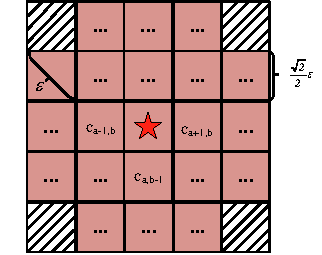
\includegraphics[width=0.6\textwidth]{fig/section5/cells.pdf}
    \caption{Potential cases of exposure}
    \label{fig:group}
\end{figure}
\paragraph{预检查策略。}
为了发现非查询组 $\mathcal{O}_{c'}$ 中所有与查询组 $\mathcal{O}_c^q$ 发生近距离接触的对象，直接计算需要 $O(|\mathcal{O}_c^q| \times |\mathcal{O}_{c'}|)$ 的时间复杂度，开销较大。为此，我们基于分组划分设计了若干预检查策略，以避免不必要的计算。具体而言，我们首先扫描 $\mathcal{O}_c^q$ 和 $\mathcal{O}_{c'}$ 中的所有位置点，分别得到其最小外包矩形 $\mathit{MBR}(\mathcal{O}_c^q)$ 和 $\mathit{MBR}(\mathcal{O}_{c'})$。公式 \ref{eq:pre-check} 定义了集合 $\{dist(l^{o_i}, l^{o_j}) \mid o_i \in \mathcal{O}_c^q, o_j \in \mathcal{O}_{c'}\}$ 的上界 $UB$ 和下界 $LB$。与 Hausdorff 距离相比，该预检查过程仅需要 $O(|\mathcal{O}_c^q| + |\mathcal{O}_{c'}|)$ 的线性时间复杂度。当上界 $UB(\mathcal{O}_c^q, \mathcal{O}_{c'})$ 小于 $\epsilon$ 时，我们可直接将 $\mathcal{O}_{c'}$ 中的所有对象视为近距离接触对象；相反，当下界 $LB(\mathcal{O}_c^q, \mathcal{O}_{c'}) > \epsilon$ 时，则可以安全地剪枝 $\mathcal{O}_{c'}$。

\begin{equation}
    \label{eq:pre-check}
        \begin{aligned}
        UB(\mathcal{O}_c^q, \mathcal{O}_{c'}) = \max (dist(\mathit{MBR}(\mathcal{O}_c^q), \mathit{MBR}(\mathcal{O}_{c'})))\\
        LB(\mathcal{O}_c^q, \mathcal{O}_{c'}) = \min (dist(\mathit{MBR}(\mathcal{O}_c^q), \mathit{MBR}(\mathcal{O}_{c'})))
        \end{aligned}
    \end{equation}

    \begin{algorithm}[!h]
        \caption{精确群体处理（EGP）算法}
        \label{alg:EGP}
        
        \Input{
        对象集合 $\mathcal{O}$；\newline
        位置流 $L_t(\mathcal{O}), L_{t+1}(\mathcal{O}), \ldots$；\newline
        查询对象集合 $\mathcal{Q} \subseteq \mathcal{O}$；\newline
        社交距离阈值 $\epsilon$；\newline
        接触时长阈值 $k$。
        }
        \Output{
        更新后的查询对象集合 $\mathcal{Q}$。
        }
        
        \textbf{初始化:}
        $\forall o \in (\mathcal{O} - \mathcal{Q})$: $cd(o) \leftarrow 0$；\newline
        $\Pi \leftarrow \emptyset$；$A \leftarrow \emptyset$；
        
        \For(\tcc*[f]{对象位置映射到网格}){each location $l_t^o \in L_t(\mathcal{O})$ of object $o$}{
            令 $c$ 为覆盖位置 $l_t^o$ 的网格单元；
        
            \If{$o \in \mathcal{Q}$}{
                $\Pi \leftarrow \{\Pi, c\}$；
                $\mathcal{O}_c^q \leftarrow \{\mathcal{O}_c^q, o\}$；
            }
            \Else{
                $\mathcal{O}_c \leftarrow \{\mathcal{O}_c, o\}$；
            }
        }
        
        \For(\tcc*[f]{处理查询单元}){each query cell $c \in \Pi$}{
            \For(\tcc*[f]{检查相邻非查询单元}){each non-query cell $c' \in SC(c)$}{
                \If{$UB(\mathcal{O}_c^q, \mathcal{O}_{c'}) \leq \epsilon$}{
                    $A \leftarrow \{A, \mathcal{O}_{c'}\}$；
                }
                \ElseIf{$LB(\mathcal{O}_c^q, \mathcal{O}_{c'}) \leq \epsilon$}{
                    $A \leftarrow \{A, ET(\mathcal{O}_c^q, \mathcal{O}_{c'})\}$；
                }
            }
        }
        
        更新 $cd(o)$；
        
        $\mathcal{Q} \leftarrow \{\mathcal{Q} \cup o \mid cd(o) \geq k\}$；
        
        \textbf{return} 更新后的 $\mathcal{Q}$；\tcp*[f]{实时结果}
        \end{algorithm}
    
        \paragraph{算法细节。}
        算法 \ref{alg:EGP} 给出了我们提出的精确群体处理（Exact Group Processing, EGP）算法的伪代码。其输入包括：对象集合 $\mathcal{O}$，位置流 $L_t(\mathcal{O})=\{l_t^o \mid o\in \mathcal{O}\}$（表示在每个时间戳 $t$ 时对象集合 $\mathcal{O}$ 的位置），查询对象集合，社交距离阈值 $\epsilon$，以及接触时长阈值 $k$。输出为更新后的查询对象集合，其中包含最新的暴露案例。
        
        在初始化阶段，所有非查询对象的接触时长 $cd(o)$ 被设置为 0（第 1 行）。在搜索过程中，我们使用 $\Pi$ 来存储至少覆盖一个查询对象的网格单元。同时，用 $A$ 表示当前发现的近距离接触对象集合。在算法开始时，$\Pi$ 和 $A$ 均被初始化为空集（第 2 行）。
        
        该算法包含两个阶段：1）群体划分阶段（第 3--11 行）；2）基于群体的近距离接触发现阶段（第 12--20 行）。在群体划分阶段，对于每一个到达的位置 $l_t^o$（对应对象 $o$），首先确定覆盖该位置的网格单元 $c$。如果 $o$ 是查询对象，则将其存入查询群体 $\mathcal{O}_c^q$，并将单元 $c$ 加入 $\Pi$；否则，将 $o$ 存入非查询群体 $\mathcal{O}_c$（第 3--11 行）。至此，所有查询群体和非查询群体均已构建完成。
        
        在近距离接触发现阶段，我们针对每一个查询群体及其相邻、具有潜在暴露风险的非查询群体，执行预检查策略（第 12--20 行）。具体而言，如果查询群体 $\mathcal{O}_c^q$ 与非查询群体 $\mathcal{O}_{c'}$ 之间距离的上界（参见公式 \ref{eq:pre-check}）不大于阈值 $\epsilon$，则将 $\mathcal{O}_{c'}$ 中的所有对象 $o$ 加入当前近距离接触集合 $A$。相反，如果其下界超过 $\epsilon$，则可以安全地剪枝 $\mathcal{O}_{c'}$，因为该群体中的任何对象都不可能与查询群体中的对象形成近距离接触。
        
        在完成群体级别的发现之后，我们进一步计算每个查询群体与其相邻、具有潜在暴露风险的非查询群体之间对象的成对距离（第 17 行）。在每一轮处理结束时，我们更新所有对象的接触时长（第 21 行）。具体地，对于所有不属于 $A$ 的对象 $o \in \mathcal{O} \setminus A$，将其接触时长重置为 0，表示在其接触时长达到阈值 $k$ 之前发生了中断。
        
        随后，对集合 $A$ 中的对象（即最新发现的近距离接触对象）更新其接触时长，并据此更新查询集合 $\mathcal{Q}$，将接触时长满足 $cd(o) \geq k$ 的对象作为最新的暴露案例加入其中（第 22 行）。最后，输出更新后的 $\mathcal{Q}$ 作为实时结果（第 23 行）。
        
        \paragraph{时间复杂度分析。}
        构建所有查询群体和非查询群体的时间复杂度为 $O(|\mathcal{O}|)$。设 $p$ 和 $q$ 分别表示每个查询群体和每个非查询群体中的对象数量，则发现近距离接触的时间复杂度为
        $O(|\Pi| \times |SC| \times p \times q)=O(|\Pi| \times p \times q)$，
        其中 $|SC|$ 为常数（参见群体划分过程）。
        
        在最坏情况下，一个网格单元可能覆盖所有查询对象，而另一个网格单元覆盖所有非查询对象（例如 $|\Pi|=1, p=|\mathcal{Q}|, q=|\mathcal{O}|$）。由于 $|SC|$ 为常数，此时每一轮运行 $EGP$ 的时间复杂度为 $O(|\mathcal{Q}||\mathcal{O}|)$。需要指出的是，在大多数实际场景中，$p$ 和 $q$ 通常远小于 $|\mathcal{Q}|$ 和 $|\mathcal{O}|$。

        \section{近似分组处理算法}

        为进一步提升暴露案例发现的效率，我们提出了一种 \underline{近似分组处理}（\underline{A}pproximate \underline{G}roup \underline{P}rocessing，AGP）算法。本节将介绍所采用的近似策略及算法细节。
        
        \paragraph{首尾优先检查策略。}
        在相邻的两个时间戳之间，可能存在大量对象彼此靠近地移动，但其中大多数对象并不能在较长时间内持续同行。若一个非查询对象在其接触时长尚未达到阈值 $k$ 之前未能持续成为近距离接触对象，则该对象不可能成为暴露案例。基于这一观察，我们提出了首尾优先检查策略。与按时间顺序逐一发现近距离接触不同，我们首先计算 $A_t$（即“尾部”）与 $A_{t-k}$（即“头部”）的交集，以获得在时间戳 $t$ 仍可能存在近距离接触的候选对象，其中 $A_t$ 表示时刻 $t$ 的近距离接触集合。对于时间区间 $[t-k+1,\, t]$，我们只需在该交集结果中进一步查找近距离接触，从而显著提升空间和时间效率。

        \begin{algorithm}[tb]
            \caption{近似分组处理算法（AGP）}
            \label{alg:AGP}
            \Input{
            对象集合 $\mathcal{O}$；\newline
            位置流 $L_t(\mathcal{O}), L_{t+1}(\mathcal{O}), \ldots$；\newline
            查询对象集合 $\mathcal{Q} \subseteq \mathcal{O}$；\newline
            社交距离阈值 $\epsilon$；\newline
            接触持续时间阈值 $k$；\newline
            跳跃步长 $m$。
            }
            \Output{实时近似暴露结果（更新后的查询集合 $\mathcal{Q}$）。}
            
            \BlankLine
            \textbf{初始化：} 对所有 $o \in (\mathcal{O}\setminus\mathcal{Q})$，令 $cd'(o)\leftarrow 0$；
            
            \If(\tcc*[f]{仅在跳跃时间点进行处理}){$t \bmod m = 0$}{
                $\Pi \leftarrow \emptyset$；$A' \leftarrow \emptyset$；
            
                \ForEach(\tcc*[f]{分组阶段}){对象 $o$ 在时刻 $t$ 的位置 $l_t^o \in L_t(\mathcal{O})$}{
                    令 $c$ 为覆盖 $l_t^o$ 的网格单元；\\
                    \uIf(\tcc*[f]{查询对象}){$o \in \mathcal{Q}$}{
                        $\Pi \leftarrow \Pi \cup \{c\}$；\\
                        $\mathcal{O}_c^q \leftarrow \mathcal{O}_c^q \cup \{o\}$；
                    }
                    \Else(\tcc*[f]{非查询对象}){%
                        $\mathcal{O}_c \leftarrow \mathcal{O}_c \cup \{o\}$；
                    }
                }
            
                \ForEach(\tcc*[f]{近邻单元扫描}){查询单元 $c \in \Pi$}{
                    \ForEach{非查询单元 $c' \in SC(c)$}{
                        $A' \leftarrow A' \cup \mathcal{O}_{c'}$；
                    }
                }
            
                \tcp{更新接触持续时间}
                更新所有对象的 $cd'(o)$；
            
                \tcp{头尾优先检查并更新查询集合}
                $\mathcal{Q} \leftarrow \mathcal{Q} \cup 
                \{\, o \mid o \in A_t \cap A_{t-k+1} \land cd'(o) \ge k \,\}$；
            }
            
            \textbf{return} 更新后的 $\mathcal{Q}$ 作为实时近似结果；
            \end{algorithm}

            \paragraph{跳跃检查。}
            给定接触时长阈值 $k$，若对象 $o$ 在连续 $k$ 个时间段 $[t_i, t_{i+k-1}]$ 内是潜在的暴露案例，并且在时间戳 $t_i$ 和 $t_{i+k-1}$ 均与至少一个查询对象发生近距离接触，则我们将对象 $o$ 视为一个近似暴露案例。
            基于近似暴露案例的定义，我们提出跳跃检查策略：
            不同于处理所有时间戳上的位置数据，我们仅在部分时间戳 $T=0,m,2m,\ldots$ 上处理位置数据，其中 $m$ 为跳跃长度。需要注意的是，当 $m=1$ 时，需要在每一个时间戳上进行处理。
            若时间戳 $t \notin T$，我们假设所有对象均为近距离接触对象。跳跃检查的目标是在不产生漏检的前提下，进一步降低计算开销。
            
            \paragraph{算法细节。}
            
            算法~\ref{alg:app} 给出了 AGP 算法的伪代码。与 EGP 相比，AGP 额外引入了跳跃长度 $m$ 作为输入参数。
            算法的输出为更新后的查询对象集合，其中包含原有查询对象以及最新发现的近似暴露案例。
            我们使用 $cd'(o)$ 表示对象 $o$ 作为潜在暴露案例的持续时长，并在算法开始时对每个非查询对象初始化 $cd'(o)$（第 1 行）。
            在算法中，仅当 $t \% m = 0$ 时，才在该时间戳上检测潜在暴露案例（第 2 行）。我们使用 $\Pi$ 来存储至少包含一个查询对象 $o\in \mathcal{Q}$ 的网格单元集合。
            我们分别用 $A$ 和 $A'$ 表示近距离接触集合和潜在暴露案例集合。
            对于对象 $o$ 在时间 $t$ 的位置 $l_t^o \in L_t(\mathcal{O})$，我们执行与 EGP 相同的操作以获得查询分组 $\mathcal{O}_c^q$ 以及非查询分组 $\mathcal{O}_c$（第 4--12 行）。
            随后，我们将位于 $SC(c)$ 中的对象视为潜在暴露案例，并相应地增加其接触时长（第 13--17 行）。
            接着，我们对不属于 $A'$ 的对象 $o$ 重置其接触时长（第 18 行）。
            对于满足 $cd'(o)\geq k$ 的对象，我们进一步检查其在时间戳 $t$ 和 $t-k+1$ 是否为近距离接触对象。若条件成立，则将其视为近似暴露案例，并将其加入查询集合 $\mathcal{Q}$（第 19 行）。
            最后，返回更新后的 $\mathcal{Q}$ 作为实时检测结果。
            
            \paragraph{时间复杂度分析。}
            分组划分过程需要 $O(|\mathcal{O}|)$ 的时间复杂度，主要差异体现在暴露案例的发现阶段。
            此外，潜在暴露案例的发现需要 $O(|\Pi|\times |SC|)=O(|\Pi|)$ 的时间。
            在最坏情况下，任意两个查询对象位于不同的网格单元中，即 $|\Pi|=|\mathcal{Q}|$。
            因此，AGP 算法每一轮的整体时间复杂度为 $O(|\mathcal{O}|+|\mathcal{Q}|)$。需要注意的是，$|\Pi|$ 的最大值为 $|\mathcal{Q}|$。

            

\section{实验研究}

\subsection{实验设置}

\paragraph{数据准备。}
我们的实验基于两个真实世界的轨迹数据集开展。第一个数据集来源于北京出租车数据集 \cite{DBLP:conf/kdd/YuanZXS11}，
包含在北京一周内跟踪到的 10,357 辆出租车的轨迹，总数据点数量约为 1,500 万。
第二个数据集采集自葡萄牙波尔图市（PT），时间跨度为 19 个月，包含超过 170 万条轨迹。
在北京数据集中，平均采样时间间隔为 177 秒，对应的平均移动距离约为 623 米；
而在波尔图数据集中，每辆出租车以 15 秒的间隔上报其位置信息。
时间戳的取值范围被限制在 24 小时之内。
我们限制经纬度范围，以保证采样位置具有足够高的空间密度。
此外，我们过滤掉采样点数量较少的轨迹，具体而言，仅保留采样点数量不少于 10 的轨迹用于实验。
为了能够在任意时间点计算对象（如出租车、行人）之间的距离，
我们通过线性插值对所有轨迹进行时间对齐，使得每个对象以固定频率返回其实时位置，
其中北京和波尔图数据集的频率分别为 10 秒和 5 秒。
最终，北京和波尔图数据集中分别包含 296,364,033 和 23,767,470 个有效位置点。
在不失一般性的前提下，我们从 $\mathcal{O}$ 中随机选取部分对象 $Q$ 作为初始查询对象。

\paragraph{对比算法。}
我们对比评估了所提出的算法，包括精确遍历算法（ET）、精确分组处理算法（EGP）以及近似算法（AGP）。
对于 AGP，默认的跳跃长度（hop length）设置为 2。
效率评估和效果评估所采用的性能指标分别为 CPU 时间以及发现的（近似）暴露案例总数。
为简化描述，我们使用 $|CE|$ 表示（近似）暴露案例的数量。
CPU 时间定义为每一轮算法运行的平均执行时间。
此外，我们还评估了 AGP 的准确性，其计算方式为真实暴露案例数量与近似暴露案例数量之比。

\paragraph{参数设置。}
默认参数设置如表 \ref{tb:para} 所示，该设置基于两个数据集的具体数据分布。
所有算法均采用 Java 实现，并在配备 AMD Ryzen 5 处理器（3.6GHz）和 32GB 内存的 Windows 10 平台上进行评测。
除非另有说明，实验结果均为在不同查询对象输入条件下进行 20 次独立实验后的平均值。
\begin{table}[tb]
    \centering
    \renewcommand\arraystretch{1.2}
    \begin{tabular}{l|rr}
    \toprule
        &\textbf{北京（Beijing）}&\textbf{波尔图（Porto）}\\
    \hline
    \hline
        经度 & [116.250, 116.550] & [-8.735, -8.156] \\
    \hline
        纬度 & [39.830, 40.030] & [40.953, 41.307] \\
    \hline
        $\epsilon$ & \{2, 4, 6, 8, 10\} & \{2, 4, 6, 8, 10\}  \\ 
        & 2 米（默认） & 2 米（默认） \\
    \hline
        $k$ & \{5, 10, 15, 20, 25\} & \{5, 7, 9, 11\} \\
        & 15（默认） & 5（默认） \\
    \hline
        $|\mathcal{Q}|$ & \{2, 4, 6, 8, 10\} $\times 10^2$  & \{2, 4, 6, 8, 10\} $\times 10^4$ \\
           & 600（默认） & 100{,}000（默认） \\
    \bottomrule
    \end{tabular}
    \caption{参数设置}
    \label{tb:para}
\end{table}

\subsection{性能评估}
\begin{figure}[tb]
    \centering
	\subfloat[北京]{
		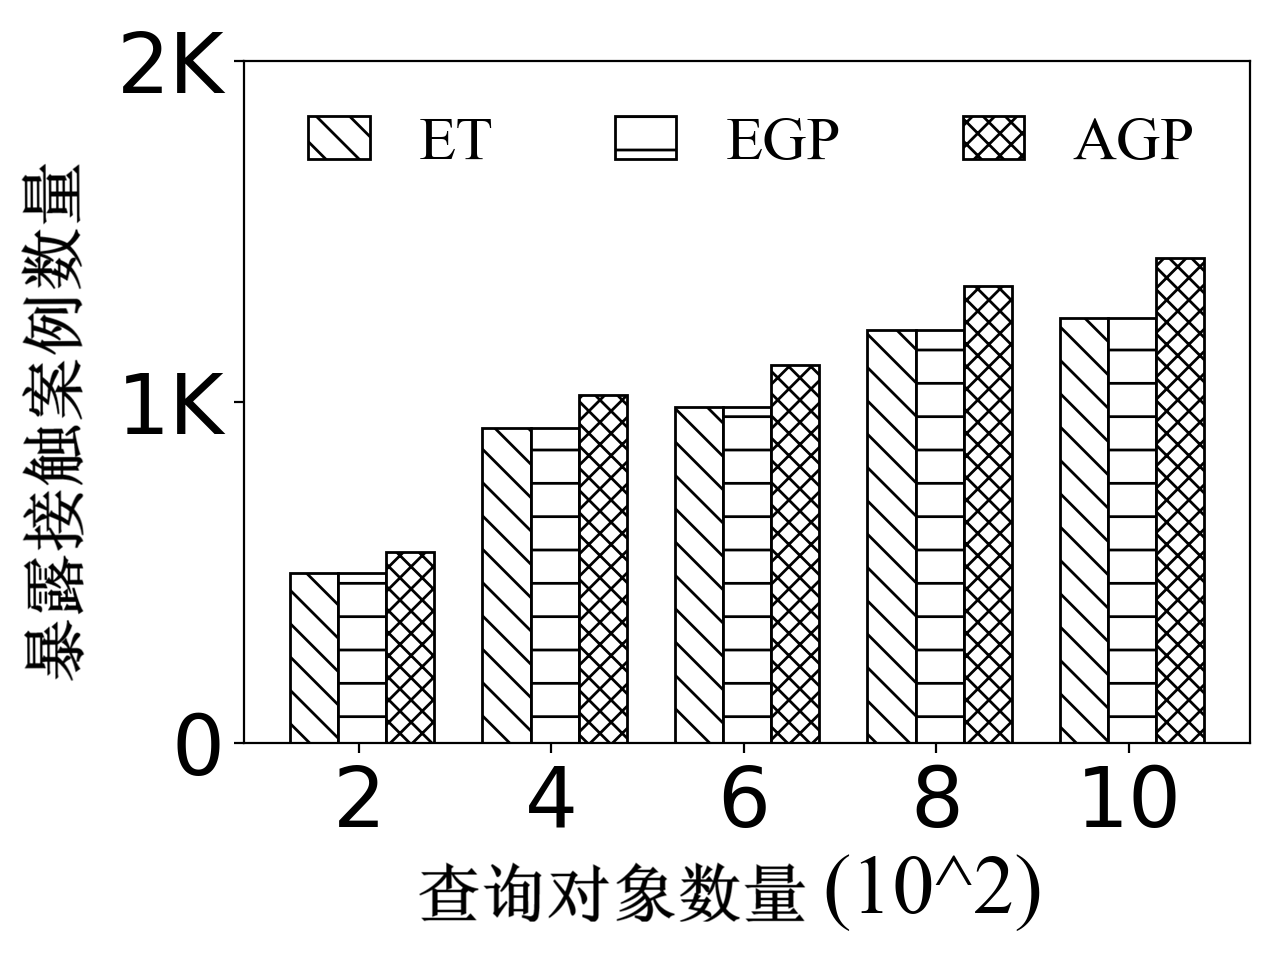
\includegraphics[width=0.4\textwidth]{fig/section5/BJ-Q-CE.png}
        \label{Beijing-Q-CE}
	}% 
    \hfill
	\subfloat[北京]{
    	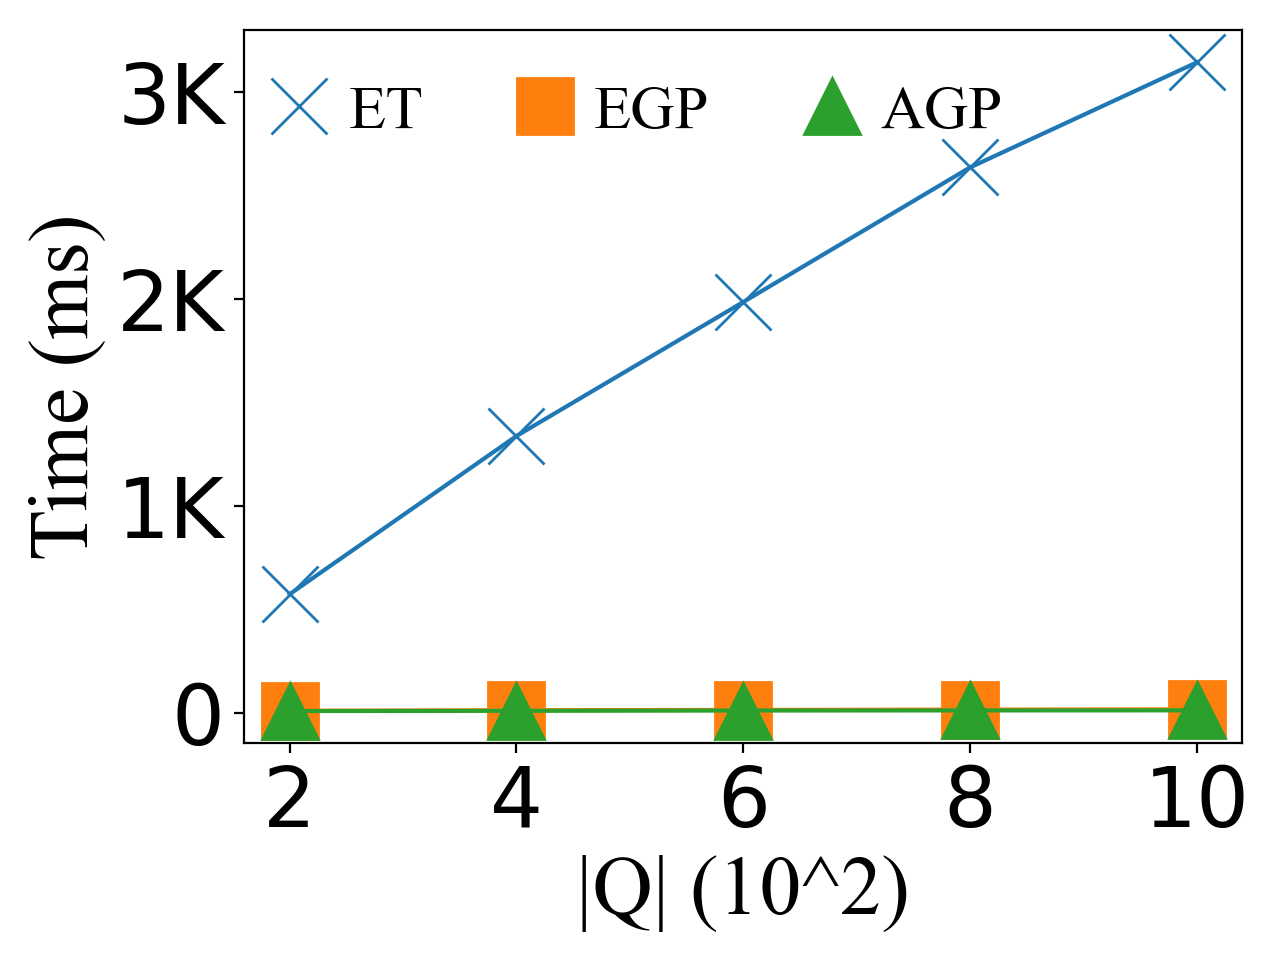
\includegraphics[width=0.4\textwidth]{fig/section5/BJ-Q-time.png}
    	\label{Beijing-Q-CPU}
	}%
	
	\subfloat[波尔图]{
		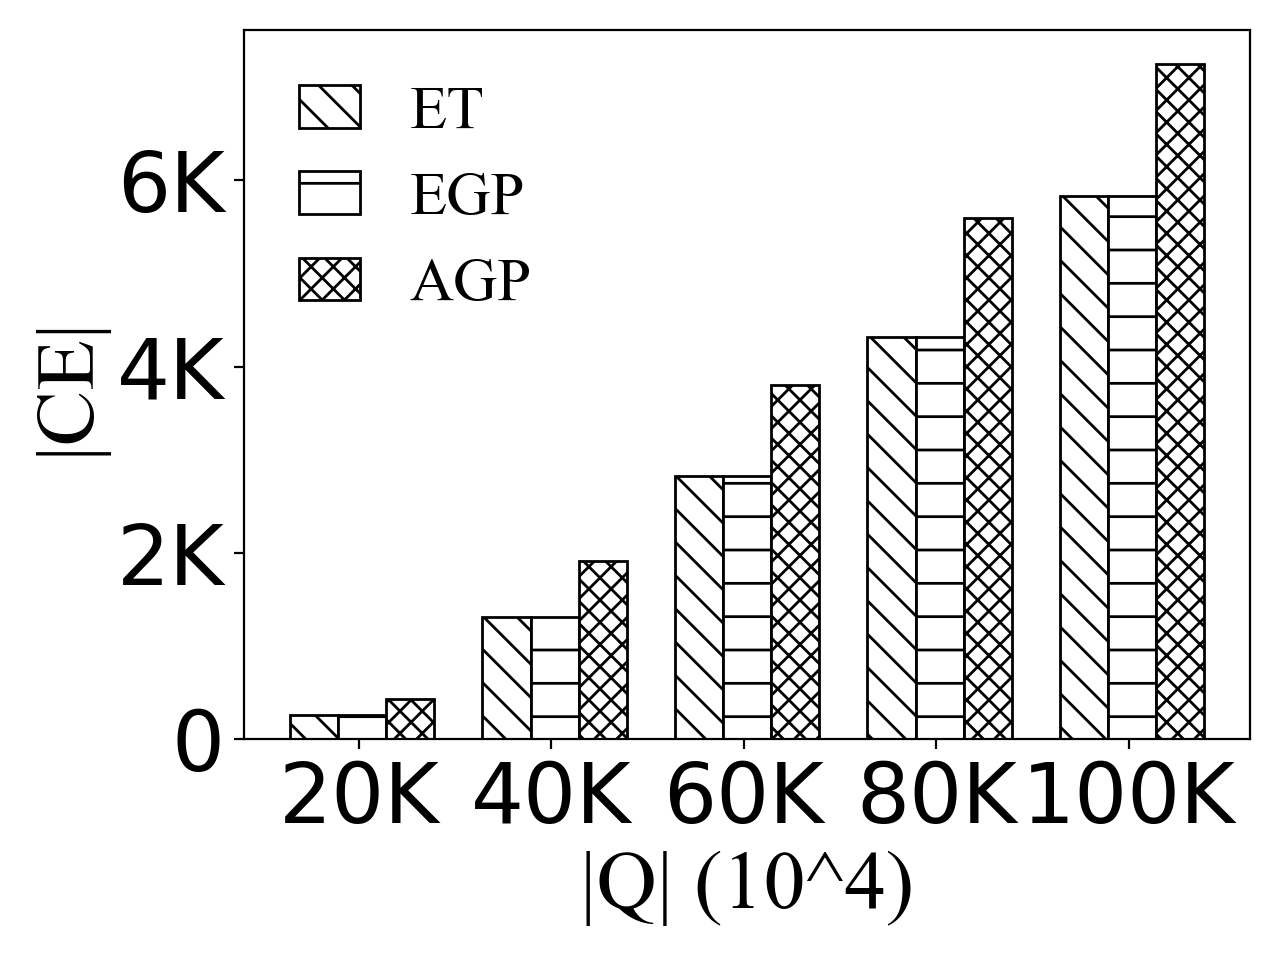
\includegraphics[width=0.4\textwidth]{fig/section5/PT-Q-CE.png}
		\label{Porto-Q-CE}
	}%
    \hfill
	\subfloat[波尔图]{
           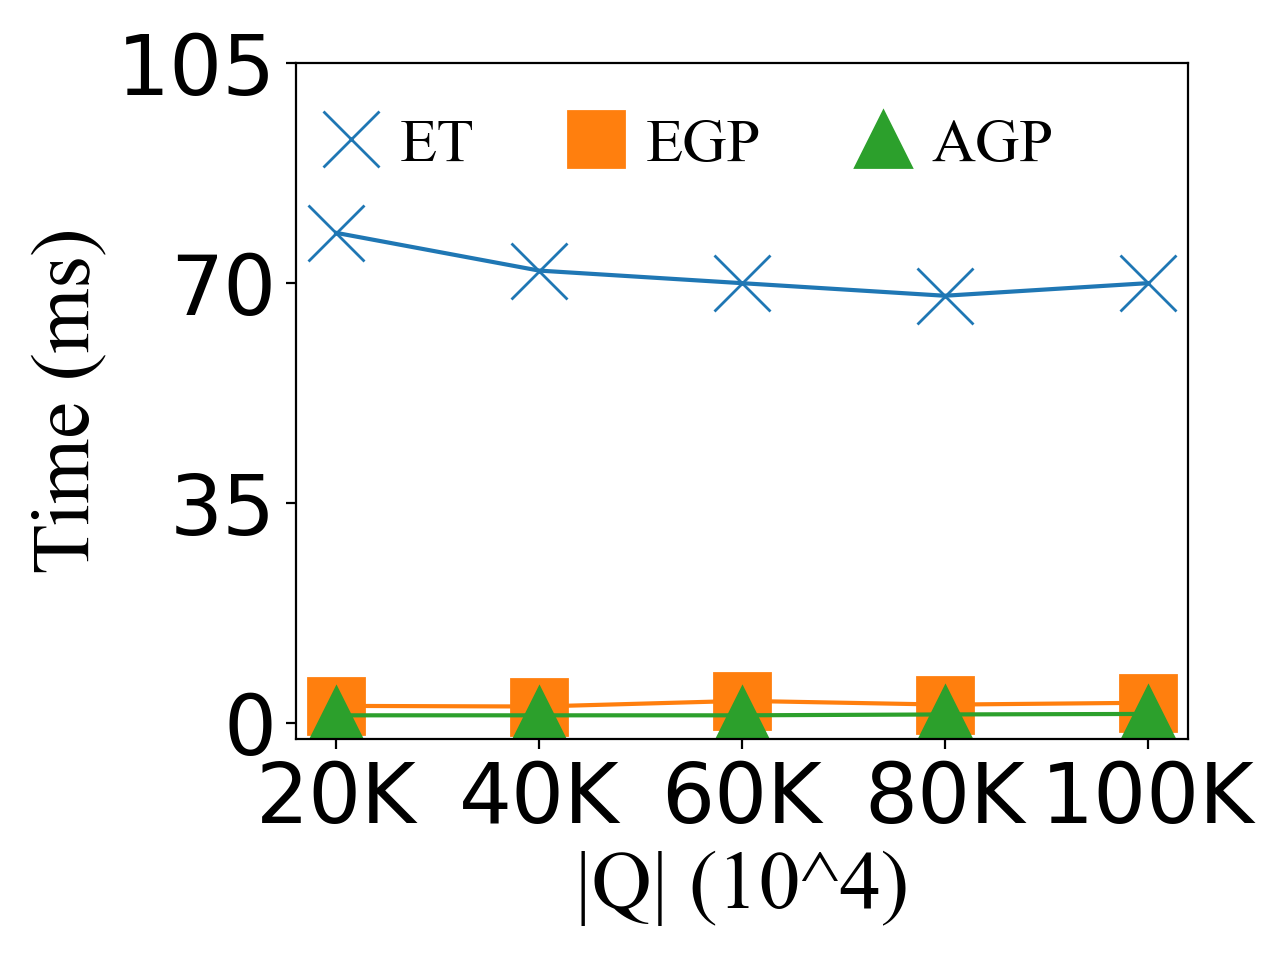
\includegraphics[width=0.4\textwidth]{fig/section5/PT-Q-time.png}
           \label{Porto-Q-CPU}
	}%
	\caption{查询对象数量的影响}
	\label{img:queryNum}
\end{figure}

\begin{figure}[htbp]
    \centering
	\subfloat[北京]{
		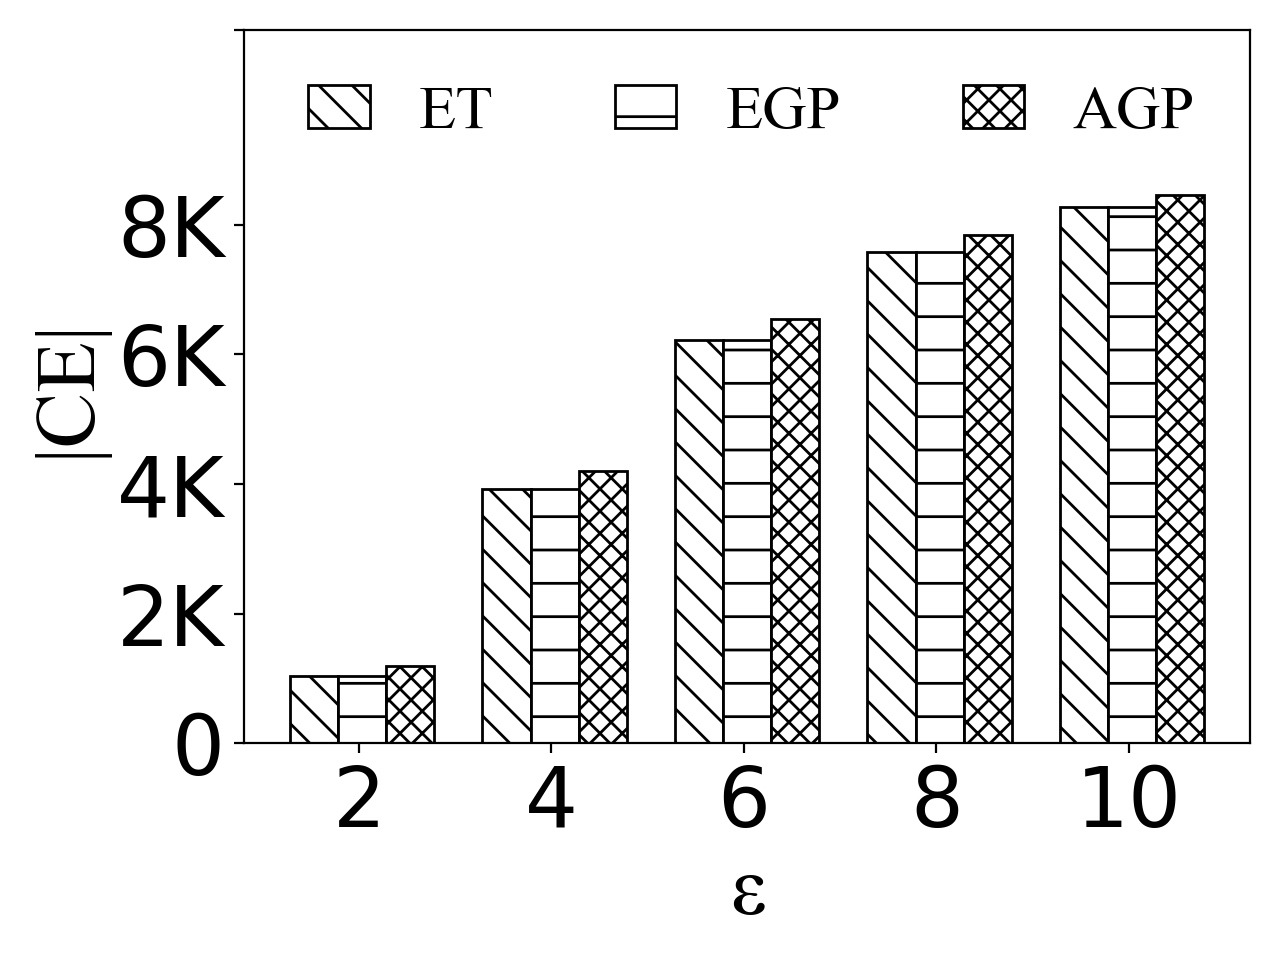
\includegraphics[width=0.4\textwidth]{fig/section5/BJ-ep-CE.png}
        \label{Beijing-ep-CE}
	}% 
    \hfill
	\subfloat[北京]{
    	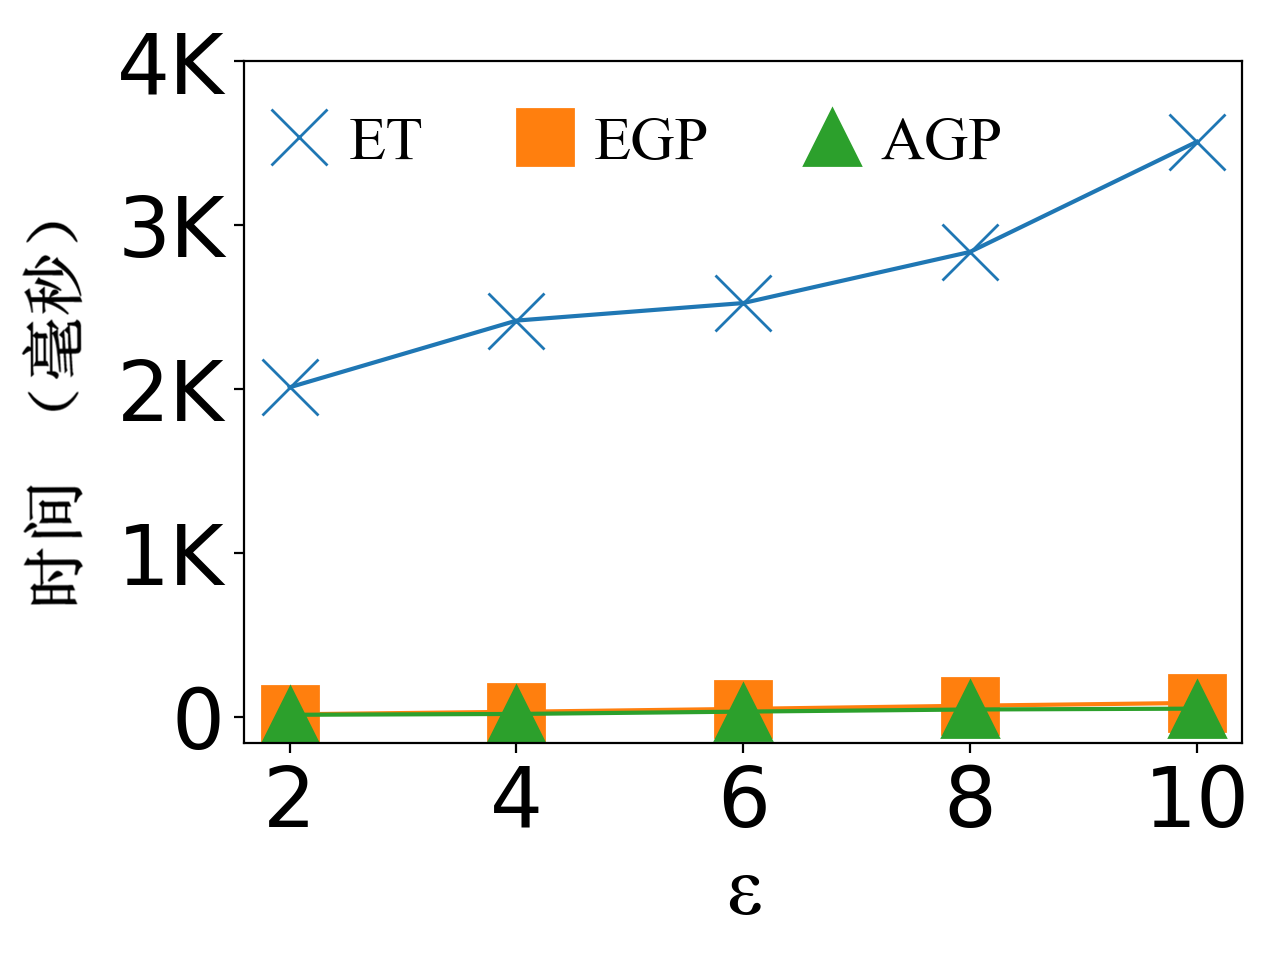
\includegraphics[width=0.4\textwidth]{fig/section5/BJ-ep-time.png}
    	\label{Beijing-ep-CPU}
	}%
	
	\subfloat[波尔图]{
		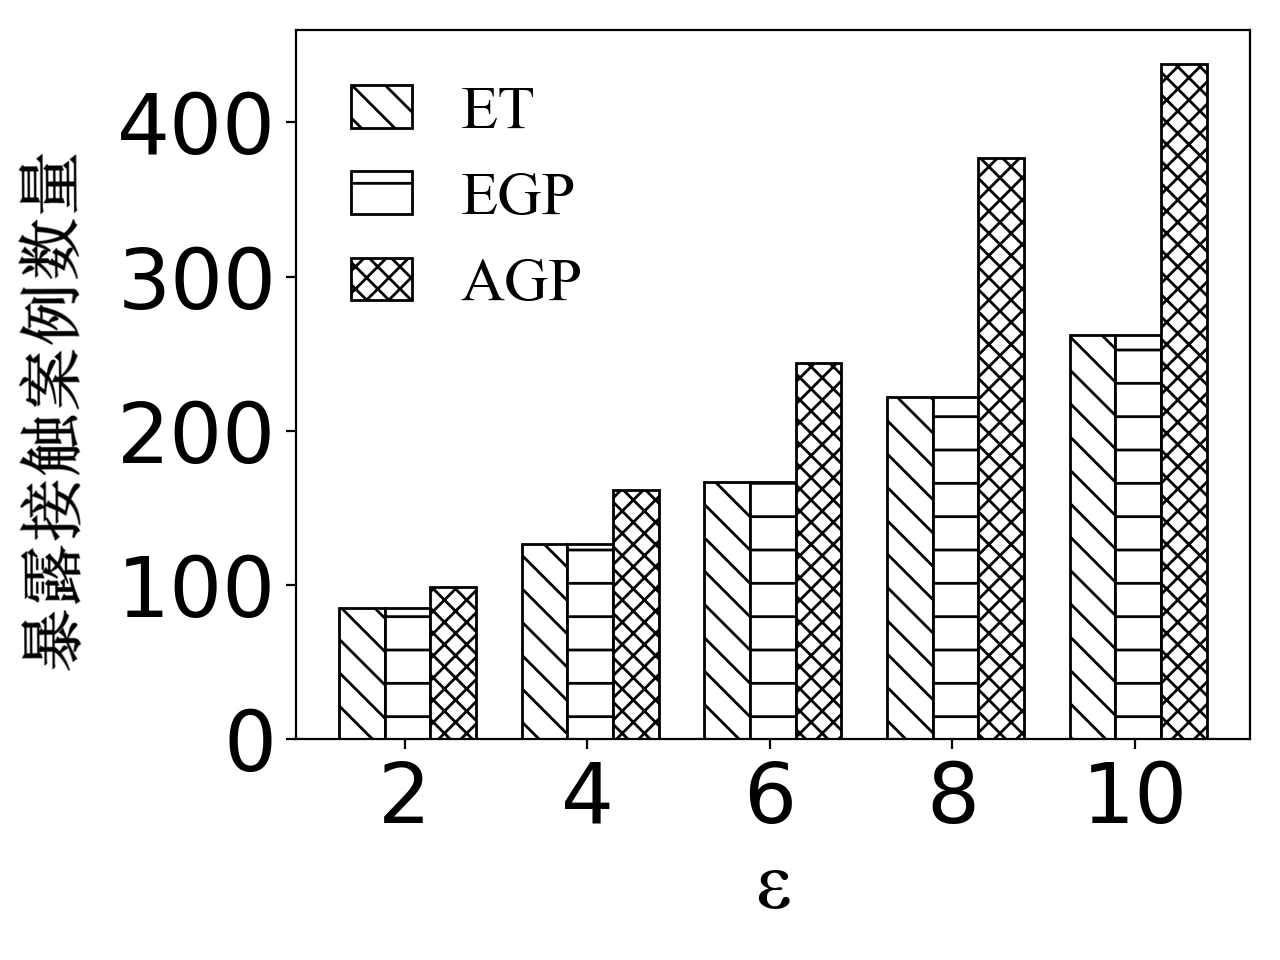
\includegraphics[width=0.4\textwidth]{fig/section5/PT-ep-CE.png}
		\label{Porto-ep-CE}
	}%
    \hfill
	\subfloat[波尔图]{
           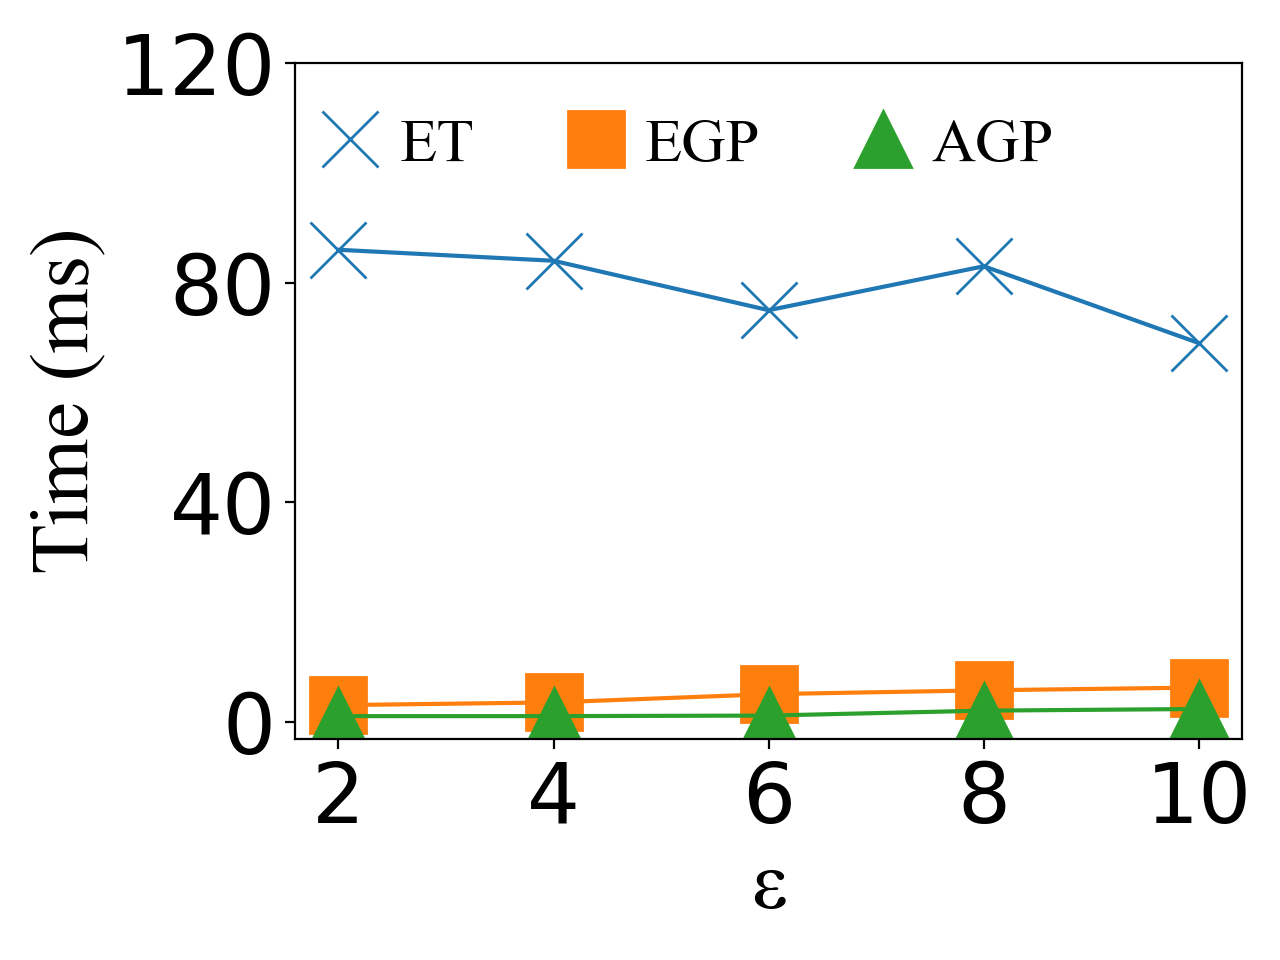
\includegraphics[width=0.4\textwidth]{fig/section5/PT-ep-time.png}
           \label{Porto-ep-CPU}
	}%
	\caption{距离阈值 $\epsilon$ 的影响}
	\label{img:ep}
\end{figure}


\paragraph{查询对象数量的影响。}
首先，我们在默认参数设置下研究查询对象数量 $|Q|$ 对所提出算法性能的影响。如图 \ref{Porto-Q-CE} 所示，在 Porto 数据集上，暴露案例数量呈现出显著的增长趋势，而在 BJ 数据集上该趋势并不明显。可以清楚地看到，ET 与 EGP 发现的暴露案例数量完全一致，这是因为它们都是精确算法。三种算法的结果总体上较为接近。如图 \ref{Beijing-Q-CPU} 和图 \ref{Porto-Q-CPU} 所示，在 CPU 时间方面，组处理算法的性能略逊于近似算法。ET 在处理北京数据集时所需的 CPU 时间超过 1{,}000 ms，这表明 ET 无法用于实时查询。相比之下，EGP 和 AGP 至少将所需 CPU 时间降低了一个数量级，充分体现了我们方法的优势。  

\paragraph{距离阈值 $\epsilon$ 的影响。}
直观上，较大的 $\epsilon$ 值意味着两个对象更容易与查询对象发生近距离接触。图 \ref{img:ep} 展示了当距离阈值 $\epsilon$ 从 2 米变化到 10 米时的性能表现。正如预期的那样，在 BJ 和 PT 数据集上，随着 $\epsilon$ 的增大，所有算法发现的暴露案例数量均随之增加。
从图 \ref{Beijing-ep-CE} 可以看出，在 BJ 数据集上，随着 $\epsilon$ 的增大，ET 与 AGP 结果之间的差异逐渐缩小；而在 PT 数据集上，这种差异则随着 $\epsilon$ 的增大而更加明显。这种现象可能归因于两种数据集在分布上的差异。值得注意的是，ET 算法的运行时间并没有呈现出明显的变化趋势，这是因为 ET 所需的计算开销在很大程度上依赖于查询对象的数量。  

\paragraph{接触持续时间 $k$ 的影响}
我们研究了接触持续时间阈值 $k$ 对算法性能的影响。较小的 $k$ 表示对象更容易被判定为暴露案例，从而导致暴露案例数量增加，并使得在每个时间快照下需要更高的 CPU 计算开销。如图 \ref{Beijing-k-CE} 和图 \ref{Porto-k-CE} 所示，当 $k$ 从 10 增加到 40 时，所有算法在北京和波尔图数据集上的暴露案例数量均显著下降。此外，从图 \ref{Beijing-k-CPU} 和图 \ref{Porto-k-CPU} 可以观察到 CPU 时间呈现出轻微的下降趋势，这是因为较大的 $k$ 会减少需要进一步检查的候选对象数量。

\paragraph{近似算法的评估}
图 \ref{img:app} 展示了在改变查询对象数量 $|Q|$ 和社交距离阈值 $\epsilon$ 时，AGP 算法的准确率表现。在北京数据集上，AGP 算法能够保持较高的准确率，并且在 $|Q|$ 和 $\epsilon$ 增加时未表现出明显的性能退化。相比之下，在波尔图数据集上，随着这些参数的增大，算法的准确率有所下降，这可能与不同数据集之间的分布特性和移动模式差异有关。

\paragraph{预检查策略的评估}
我们将不采用预检查策略的 EGP 方法记为 \textit{EGP*PC}。如图 \ref{img:precheck} 所示，在改变查询对象数量的情况下，EGP 在北京和波尔图数据集上的 CPU 时间始终低于 EGP*PC。这一结果清楚地表明，所提出的预检查策略能够有效减少不必要的计算开销，从而提升整体执行效率。

\section{本章小结}
我们提出并研究了一种新的暴露搜索问题，用于在轨迹位置流中发现暴露事件（CES 问题）。针对该问题，我们提出了两种高效算法，并设计了相应的预检查策略以提升整体计算效率。大量实验结果表明，所提出的方法在效率和有效性方面均表现优异，且预检查策略能够有效避免不必要的计算开销。
	% \chapter{一种面向时空运动范围的轨迹相似性连接方法}

\section{引言}
随着智能手机等 GPS 设备的普及，对移动对象的查询问题受到了广泛关注，相关研究涵盖了连接（join）、范围查询、$k$NN 查询、相似性查询等多种类型。然而，由于采样频率不一致、位置采样可能存在误差，以及相邻采样点之间位置不可观测等因素，这类查询面临着诸多挑战。现有的相似性连接方法通常依赖于离散的位置采样点，难以刻画移动过程中的不确定性，从而可能遗漏具有实际意义的交互行为。

为了解决上述局限性，本文提出了一种新的方法——Intersection Similarity Join（IS-Join），该方法并非基于位置邻近性，而是根据对象运动范围的重叠程度来识别对象对。我们将运动范围定义为对象在给定时间段内可能经过的空间区域，并进一步提出了一种交集相似性度量来量化不同对象运动范围之间的重叠程度。

为了高效处理 IS-Join 查询，我们设计了一种带有重划分策略的 Hybrid Ball-tree 索引结构，以实现可扩展的候选对象过滤。此外，我们还引入了预检查（pre-checking）和剪枝（pruning）技术，以进一步降低计算开销。基于两个真实轨迹数据集的大量实验结果表明，IS-Join 在性能上显著优于精心设计的对比方法，运行时间最多可降低至原来的 $1/3$（即实现最高约 $3\times$ 的加速）。该研究为城市出行分析、交通监测、野生动物追踪以及接触追踪等应用场景开辟了新的可能性。
\subsection{研究背景与意义}
相似移动对象对的匹配问题，通常称为相似性连接（similarity join），是数据管理中的一项基础功能。该领域的现有研究工作~\cite{DBLP:journals/pvldb/Xu0B20,DBLP:journals/information/AlarabiBHA21,DBLP:journals/tkde/ShangCZJWK19,DBLP:journals/vldb/ShangCWJZK18,ding2025parallel} 通常将移动对象建模为一系列带时间戳的位置采样点，并基于这些采样点之间的空间邻近性来度量对象间的相似性。

然而，在真实场景中，出于隐私保护、商业因素、数据缺失以及部署成本高昂等原因，移动对象往往只能以较低的采样频率进行观测~\cite{DBLP:journals/air/KongCHWX23}，这使得相邻观测之间的位置信息不可获取。为了引入更高的灵活性，已有研究通过最小外接矩形（minimum bounding rectangle, MBR）来表示对象，并采用基于速度的表示模型来刻画其运动行为~\cite{DBLP:conf/icde/SistlaWCD97,DBLP:conf/sigmod/PatelCC04,DBLP:conf/sigmod/SaltenisJLL00,DBLP:conf/icde/ZhangLRB08,DBLP:journals/vldb/ZhangQLWW12}。另一类方法~\cite{DBLP:conf/mdm/BakalovHKT05} 则利用分段聚合近似（piecewise aggregate approximation, PAA）~\cite{DBLP:conf/vldb/YiF00} 将轨迹表示为符号序列，即将轨迹片段映射为来自预定义字母表的符号。

尽管上述方法在一定程度上提升了建模能力，现有表示方式仍然难以刻画采样点之间的运动过程，这一问题在稀疏采样轨迹场景下尤为突出。由此可能导致本应满足条件的结果对象对被错误地遗漏。因此，如何有效建模移动对象之间的运动交集关系，以及在海量移动对象数据下如何高效地发现所有交集，仍然是一个有待解决的开放性挑战。

在此背景下，我们提出了面向移动对象的交集相似性连接（Intersection Similarity Join，IS-Join）问题，通过引入运动范围来刻画对象在相邻观测样本之间可能访问的位置。具体而言，我们将对象的运动范围定义为其在某一时间点或给定时间区间内可能到达的空间区域。两个对象之间的交集相似性由其运动范围内特征的重叠程度来确定。

给定表 \texttt{MovingObject} 中的一组对象以及相似性阈值 $\theta$，我们以类似 SQL 的形式定义 IS-Join，如下所示~\footnote{为便于表示，我们以自连接（self-join）的形式定义 IS-Join。需要注意的是，本文提出的方法同样支持非自连接（non-self join）场景。}。

\begin{adjustwidth}{0.5in}{0in} \texttt{SELECT $o.id, o'.id$\\ FROM MovingObject AS $o$, MovingObject AS $o'$\\ WHERE $o.id<o'.id$ AND $IS(o,o',I) \geq \theta$} \end{adjustwidth}

每个对象 $o$ 由一个 $id$ 属性、两个位置坐标属性以及两个时间戳属性来表征，其中时间戳表示对象访问对应位置的时间。条件 $o.id<o'.id$ 用于避免重复比较。函数 $IS(o,o',I)$ 用于度量对象 $o$ 与 $o'$ 在时间区间 $I$ 内基于各自运动范围中特征重叠程度的交集相似性。参数 $\theta$ 为预先设定的相似性阈值。

IS-Join 问题面向多种应用场景，例如疾病防控、轨迹数据清洗、拼车推荐以及交通拥堵预测等~\cite{DBLP:journals/ral/VishnuARMB23,DBLP:conf/ijcai/LiCS20}。下面我们将讨论若干潜在的应用场景。



\textit{场景 1 —— 城市交通监测。} 特征集合可以包括道路路段、交叉路口以及交通信号灯等要素。交集相似性刻画了两辆车辆经历相似交通状况的可能性，有助于拥堵预测与交通优化。对于兴趣点（POI）和道路交叉口等点状特征，我们为每一个点分配一个唯一的 ID。为了将类似的方法应用于道路路段，我们将道路划分为等长度的子路段，并为每个子路段分配唯一的 ID。

\textit{场景 2 —— 野生动物迁徙。} 所定义的运动范围通过考虑栖息地、水源以及迁徙路线等特征，有助于识别共享的迁徙通道。此外，运动范围在节能的数据采集与准确的交互检测之间提供了一种折中方案~\cite{forrest2022moving}。

\textit{场景 3 —— 接触追踪。} 所定义的运动范围能够对潜在的接触事件进行估计，从而提升流行病监测系统的有效性。交集相似性可以帮助用户评估其感染风险，这在新冠疫情期间对于降低感染传播具有重要价值~\cite{DBLP:conf/ijcai/LiCSWLK022}。


  



\begin{figure}[htb]
    \centering
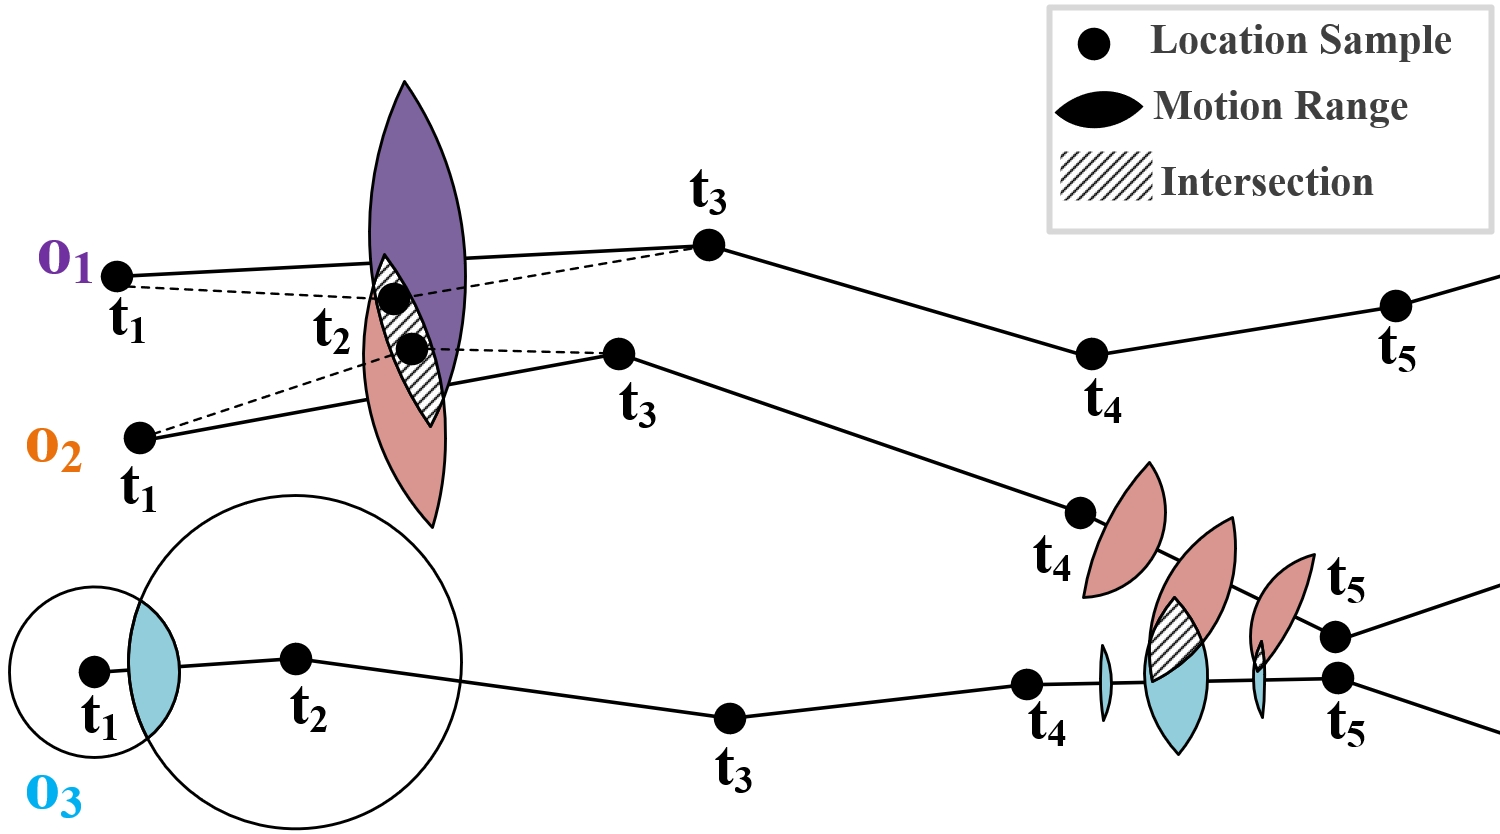
\includegraphics[width=1\columnwidth]{fig/section6/intro.png}
    \caption{IS-Join问题示例}
    \label{fig:intro}
\end{figure}

\textit{示例。} 如图~\ref{fig:intro} 所示，考虑三个移动对象 $o_1, o_2$ 和 $o_3$，它们在时间戳 $t_1$ 至 $t_5$ 之间均具有位置采样点。为简化说明，假设这些位置采样在时间上是对齐的。对象 $o_1$ 和 $o_2$ 在 $t_2$ 时刻的位置采样要么缺失，要么噪声过大而无法使用。如果仅通过判断位置采样之间的距离是否小于给定阈值来执行相似性连接，我们可能会错误地认为在时间区间 $[t_1, t_3]$ 内 $(o_1, o_2)$ 不是一个满足条件的结果对，尽管它们在 $t_2$ 时刻的实际距离可能低于该阈值。

通过考虑对象的运动范围，可以避免这种错误排除。以 $o_3$ 在 $t_1$ 和 $t_2$ 时刻的位置为例，$o_3$ 在时间点 $t\in[t_1,t_2]$ 内的运动范围为一个透镜形区域，其具体定义将在第~\ref{sec:statement} 节中给出。对象 $o_1$ 和 $o_2$ 在时间点 $t\in(t_1,t_3)$ 内的运动范围分别以紫色和棕色的透镜形区域表示。可以观察到，$o_1$ 与 $o_2$ 的运动范围在阴影区域内发生重叠，这表明它们可能存在潜在的位置交集。

接下来，我们关注时间区间 $[t_4, t_5]$。图中展示了 $o_2$ 和 $o_3$ 在区间 $[t_4,t_5]$ 内若干离散时间点上的一系列运动范围。区间 $[t_4,t_5]$ 的交集相似性被定义为该区间内各离散时间点交集相似性的平均值，具体定义将在后文的问题描述中进一步说明。给定一个时间区间和相似性阈值，IS-Join 问题旨在识别并返回在该时间区间内交集相似性大于或等于所给阈值的所有对象对。

据我们所知，这是首个在移动对象相似性连接研究中显式引入运动范围的工作。为了使 IS-Join 在实际中具有可行性，其算法必须在海量数据集上具备高效性和可扩展性。然而，IS-Join 问题的求解面临两个关键挑战。首先，在一个连续时间区间内计算精确的交集相似性在实际中是不可行的，因为这需要处理无限多个时间点。其次，现有的连接算法主要针对其他类型的查询而设计，无法直接支持 IS-Join。实验结果表明，即使在小规模数据集上，简单地改造这些方法也会导致严重的效率问题。为此，我们提出了一种由时间区间运动范围引导的解决方案。具体而言，我们设计了一种基于 HBall-tree 的连接算法，结合有效的重划分与剪枝技术，相较于精心设计的基线方法，平均运行时间可降低约 3 倍。


本文的主要贡献总结如下。

\begin{itemize}
\item 我们提出了一种新的问题——交集相似性连接（Intersection Similarity Join，IS-Join），并研究了可用于求解该问题的现有技术。不同于以往基于离散位置采样点邻近性来识别相似对象对的方法，本文首次识别运动范围感知相似性超过给定阈值的对象对。
\item 我们提出了一种由时间区间运动范围引导的高效 IS-Join 求解方案。为此，本文设计了一种混合 Ball-tree（Hybrid Ball-tree，HBall-tree）索引结构及其配套的剪枝增强技术。HBall-tree 能够高效地识别候选对象对，而剪枝增强技术则在处理早期阶段剔除不满足条件的对象对，从而显著提升查询性能。
\item 我们在两个真实世界数据集上进行了大量实验，对所提出的解决方案进行了深入分析，并验证了该方法在性能上显著优于精心设计的基线方法。
\end{itemize}

\subsection{相关工作}
\subsection{移动对象索引}
移动对象通常被表示为带时间戳的位置采样点~\cite{DBLP:conf/www/ZhengZXM09,DBLP:journals/vldb/LiNHLXZ23,DBLP:journals/debu/ZhengXM10}。R-tree~\cite{DBLP:conf/sigmod/Guttman84,DBLP:conf/sigmod/BrinkhoffKS93} 和 KD-tree~\cite{DBLP:journals/cacm/Bentley75,DBLP:journals/pvldb/ZhangCJOZ09} 是支持高效移动对象查询的两类经典索引结构。这类索引中的每个内部节点对应一个矩形区域，其子树包含位于该区域内的数据点。此外，M-tree~\cite{DBLP:conf/sebd/CiacciaPRZ97,DBLP:conf/vldb/CiacciaPZ97} 和 Ball-tree~\cite{DBLP:journals/jmlr/LiuMG06} 被设计用于高效处理圆形区域内的查询。Omohundro~\cite{omohundro1989five} 通过比较多种 Ball-tree 的构建方法，研究了构建时间与树结构质量之间的权衡关系。为提升索引结构的平衡性，Dolatshah 等人~\cite{DBLP:journals/corr/DolatshahHM15} 利用主成分分析来改进空间划分方式，从而确定更优的划分轴。另一项相关研究~\cite{DBLP:conf/dasfaa/ChaoHLZ021} 提出了面向移动对象的广义接触搜索查询。Zhang 等人~\cite{DBLP:conf/edbt/ZhangRSL21} 研究了接触相似性查询，并提出了用于索引的 ``UTM-tree''。然而，现有工作尚未基于运动范围来研究接触追踪问题，而这一点正是本文所关注的核心内容。

\subsection{轨迹相似性连接}
大量研究致力于轨迹相似性搜索与连接问题~\cite{DBLP:journals/vldb/LiangYWLCXL24,li2023relaxed,DBLP:journals/vldb/NutanongZTK10,DBLP:journals/vldb/WardH0Q14,chang2024trajectory,DBLP:conf/kdd/HanWYS021}。在这些研究中，Shang 等人~\cite{DBLP:journals/vldb/ShangCWJZK18} 采用线性组合的方式融合空间相似性与时间相似性。为降低系统负载，已有工作提出了基于速度的表示方法~\cite{DBLP:conf/icde/SistlaWCD97,DBLP:conf/sigmod/PatelCC04,DBLP:conf/sigmod/SaltenisJLL00}。Ding 等人~\cite{DBLP:journals/tkde/DingZWLBZL21} 提出了一种数据驱动的方法，利用真实历史轨迹数据挖掘实际可达区域来刻画问题。为了支持更灵活的轨迹相似性定义，Bakalov 等人~\cite{DBLP:conf/mdm/BakalovHKT05} 采用分段聚合近似（Piecewise Aggregate Approximation，PAA）~\cite{DBLP:conf/vldb/YiF00} 将轨迹表示为符号序列，并将 PAA 片段映射为来自预定义字母表的符号。他们构建了一种紧凑索引，用于高效评估近似连接，并通过后过滤步骤在加载最少轨迹数据的情况下对查询结果进行精化。Chen 等人~\cite{DBLP:conf/gis/ChenP09} 提出了一个通用的轨迹连接框架，涵盖距离连接和 $k$ 最近邻连接。此外，Tampakis 等人~\cite{DBLP:journals/tsas/TampakisDPT20} 提出了一种子轨迹连接查询，用于检索所有“最大化”的相似轨迹片段，从而识别“最大匹配”的子轨迹。尽管上述研究将相似性概念扩展到了单纯位置采样邻近性之外，但据我们所知，尚无工作研究基于运动范围的交集相似性连接问题，因此其现有解决方案并不适用于本文所提出的 IS-Join 问题。

\subsection{研究内容与挑战}
\subsection{研究成果与贡献}






\section{问题描述}


在本节中，我们首先定义移动对象的运动范围以及移动对象之间的交集相似性。随后，引入放宽交集相似性的概念，并对交集相似性连接问题进行形式化定义。本文中使用的主要符号汇总于表~\ref{tab:notation}。


\begin{table}[b]
    \centering
    \setlength{\tabcolsep}{8pt}% column separation
    \renewcommand{\arraystretch}{1}%row space 
    \begin{tabular}{ll}
        \hline
		\bfseries 符号 & \bfseries 含义 \\
        \hline
        $o$ & 一个移动对象  \\ 
        $s$ & 一个带时间戳的位置采样点  \\ 
        $[x,y],t$ & 坐标 / 时间戳  \\
        $I$ & 一个时间区间  \\ 
        $MR(\cdot)$ & 对象的运动范围 \\ 
        $dist(\cdot)$ & 距离度量函数 \\
        $\mathcal{F}(\cdot)$ & 运动范围的特征集合 \\ 
        $IS(\cdot)$ & 交集相似性度量\\
        $\theta$ & 交集相似性阈值 \\
        $\epsilon$ & 放宽划分参数 \\
        $T^\epsilon$  & 采样时间戳集合 \\
        $\mathcal{A}, \mathcal{B}$ & 两个移动对象集合  \\
        $\mathcal{R}$ & IS-Join 的结果集合 \\
        \hline
    \end{tabular}
    \caption{符号说明汇总}
    \label{tab:notation}
\end{table}




\begin{definition}[带时间戳的位置采样]
移动对象的一个带时间戳的位置采样表示为 $s=([x,y],t)$，其中 $[x,y]$ 表示空间坐标，$t$ 表示该位置被访问的时间戳。
\end{definition}


\begin{definition}[时间点运动范围]
\label{defi: point motion}
给定移动对象 $o$ 的两个位置采样点 $s_i = ([x_i, y_i], t_i)$ 和 $s_{j}=([x_j,y_j], t_j)$，以及最大速度 $v_{max}$，对象 $o$ 在时间 $t$（其中 $t \in [t_i, t_j]$）处的运动范围记为 $MR(o, t)$，其计算方式如公式~\ref{eq:timestamped motion range} 所示。函数 $dist(\cdot)$ 表示两个位置之间的距离度量。该运动范围呈透镜形状，如图~\ref{fig:lens} 所示，其两个半径 $r_i$ 和 $r_j$ 分别为 $v_{max}\cdot (t-t_i)$ 和 $v_{max}\cdot (t_j-t)$。
\begin{equation}    
\label{eq:timestamped motion range}
\begin{aligned}
MR(o,t) = \{ (x,y) \mid dist((x,y),(x_i,y_i)) \leq v_{max}\cdot(t-t_i)  \wedge \\ 
dist((x,y),(x_j,y_j)) \leq v_{max}\cdot(t_j-t)\}
\end{aligned}
\end{equation}
\end{definition}



\begin{figure}
    \centering
    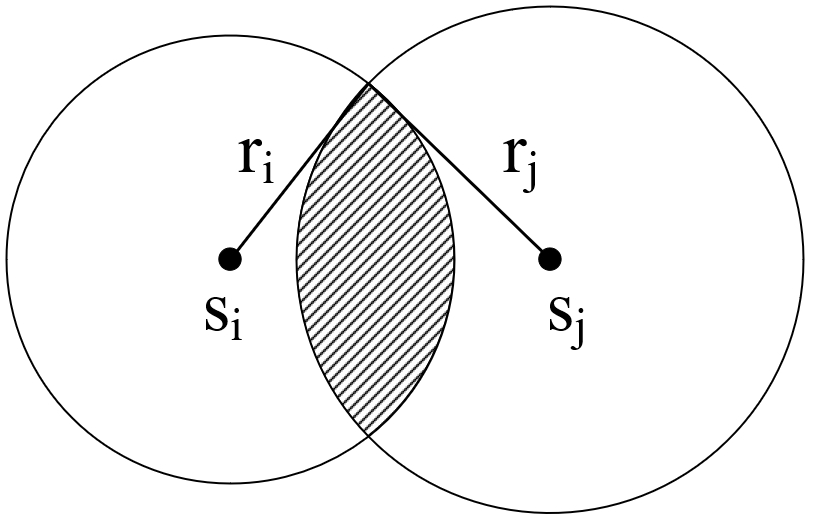
\includegraphics[width=0.5\columnwidth]{fig/section6/lens.png}
    \caption{Illustration of time-point motion range}
    \label{fig:lens}
\end{figure}


时间点运动范围的建模方式与已有研究保持一致~\cite{DBLP:conf/ssd/PfoserJ99,DBLP:conf/edbt/ZhangRSL21,trajcevski2010uncertain}。本文采用最大速度进行建模，以确保所估计的运动范围能够完全覆盖对象的真实运动轨迹。特别地，在采样时间戳处，对应的运动范围即退化为该时间戳的位置采样点本身。对于采样时间间隔异常较长（例如达到数小时）的对象，不在本文的分析范围之内。


\begin{definition}[运动范围特征]\label{defi: feature set}
设 $\mathcal{F}(o,t)$ 表示位于运动范围 $MR(o,t)$ 内的一组特定特征。示例包括运动范围的面积、范围内的兴趣点、经过的道路路段，以及地理空间区域或环境因素等。
\end{definition}



\begin{definition}[时间点交集相似性]\label{defi: point similarity}
对象 $o$ 与 $o'$ 在时间 $t$ 处的时间点交集相似性记为 $IS(o,o',t)$，其定义如公式~\ref{eq: time-point intersection similarity} 所示，用于度量二者特征集合之间的重叠程度。其中，$|\mathcal{F}(\cdot)|$ 表示位于 $MR(o,t)$ 内的特征集合大小，$\cap$ 表示特征集合之间的交集，该交集可根据具体应用场景表示共享的兴趣点、共同经过的道路路段，或重叠的运动范围区域等。相似性取值范围为 $[0,1]$，其中 1 表示特征集合完全重叠，0 表示不存在重叠。
%
\begin{equation}
    \label{eq: time-point intersection similarity}
    IS(o,o',t) = 
    \frac{|\mathcal{F}(o,t) \cap \mathcal{F}(o',t)|}{|\mathcal{F}(o,t)|}\times \frac{|\mathcal{F}(o,t) \cap \mathcal{F}(o',t)|}{|\mathcal{F}(o',t)|}
\end{equation}

\end{definition}

时间点交集相似性的定义基于如下考虑。首先，$MR(o,t)$ 描述了对象 $o$ 在时间 $t$ 处可能占据的位置范围，而 $\mathcal{F}(\cdot)$ 则表示该运动范围内的相关特征集合。采用乘积形式意味着两个因子都必须足够大，交集相似性才会取得较高值，从而保证只有在运动范围重叠程度高且特征相似性强这两个条件同时满足时，相似性得分才会较高。相比之下，经典的 Jaccard、取平均或取最小值等方法难以有效平衡运动范围重叠与特征相似性这两个方面。因此，$IS(o,o',t)$ 通过评估二者特征集合的重叠情况，刻画了对象 $o$ 与 $o'$ 之间发生交互的可能性。
 
\begin{definition}[时间区间交集相似性]\label{defi:interval similarity}
给定起始时间为 $t_s$、结束时间为 $t_e$ 的时间区间 $I$，我们将对象 $o$ 与 $o'$ 在区间 $I$ 上的交集相似性定义为该区间内时间点交集相似性的平均值，如公式~\ref{eq:interval intersection similarity} 所示。
\begin{equation}
    \label{eq:interval intersection similarity}
    IS(o,o',I) =\frac{\int_{t_s}^{t_e} IS(o,o',t) \, dt}{t_e-t_s}
\end{equation}
\end{definition}

计算时间区间交集相似性并非易事，因为由于时间区间的连续性，需要在无限多个时间点上评估时间点交集相似性。为在实际应用中对大规模移动对象数据提供一种可扩展的近似计算方式，并在不显著损失一般性的前提下，本文提出了一种放宽的定义。




\begin{definition}[$\epsilon$-放宽的时间区间交集相似性）]\label{defi:relaxed similarity}
给定一个较小的常数 $\epsilon$，我们对时间区间 $I=[t_s,t_e]$ 进行 $\epsilon$-采样，通过均匀采样得到一组时间点 $T^\epsilon=\{t_1^\epsilon,\ldots,t_m^\epsilon\}$，其中 $t_1^\epsilon=t_s$，$t_m^\epsilon=t_e$，且满足 $t_{i+1}^\epsilon-t_i^\epsilon=\epsilon$。随后，我们将 $\epsilon$-放宽的时间区间交集相似性定义为对象 $o$ 与 $o'$ 在所有采样时间点 $t^\epsilon\in T^\epsilon$ 上的时间点交集相似性的平均值，记为 $IS(o,o',I,\epsilon)$，其计算方式如公式~\ref{eq:relaxed similarity} 所示。
\begin{equation}
    \label{eq:relaxed similarity}
     IS(o,o',I,\epsilon) = \frac{\sum_{i=1}^{m} IS(o,o',t_i^\epsilon)}{m}
\end{equation}
\end{definition}


从本质上看，时间区间相似性的计算需要对多个时间点上的时间点交集相似性进行评估。在下文中，如无特殊说明，为表述简洁起见，我们使用“交集相似性”来指代 $\epsilon$-放宽的交集相似性。当 $\epsilon$ 趋近于 0 时，$IS(o,o',I,\epsilon)$ 将收敛到 $IS(o,o',I)$。

\textit{示例。}
图~\ref{fig:relaxed similarity example} 给出了一个时间区间交集相似性计算的示例。考虑时间区间 $I=(t_4,t_5)$，令 $\epsilon=|I|/4$，则采样得到的时间集合为 $T^\epsilon={t_4,t_4+\epsilon,t_4+2\epsilon,t_4+3\epsilon,t_5}$。两个移动对象 $o_2$ 和 $o_3$ 在 $T^\epsilon$ 中各采样时间点处均具有对应的时间点运动范围。在时间点 $t_4$ 和 $t_4+\epsilon$ 处，两者的运动范围不存在交集，因此 $IS(o_2,o_3,t_4)=0$ 且 $IS(o_2,o_3,t_4+\epsilon)=0$。在 $t_5$ 时刻，$o_2$ 与 $o_3$ 的位置采样点相同，从而得到 $IS(o_2,o_3,t_5)=1$。因此，区间 $I$ 上的 $\epsilon$-放宽时间区间交集相似性可计算为 $(0+0+IS(o_2,o_3,t_4+2\epsilon)+IS(o_2,o_3,t_4+3\epsilon)+1)/5$。其中，$IS(o_2,o_3,t_4+2\epsilon)$ 和 $IS(o_2,o_3,t_4+3\epsilon)$ 的取值依据公式~\ref{eq: time-point intersection similarity} 计算，该公式能够适应不同应用场景下的具体需求。


\begin{figure}
    \centering
    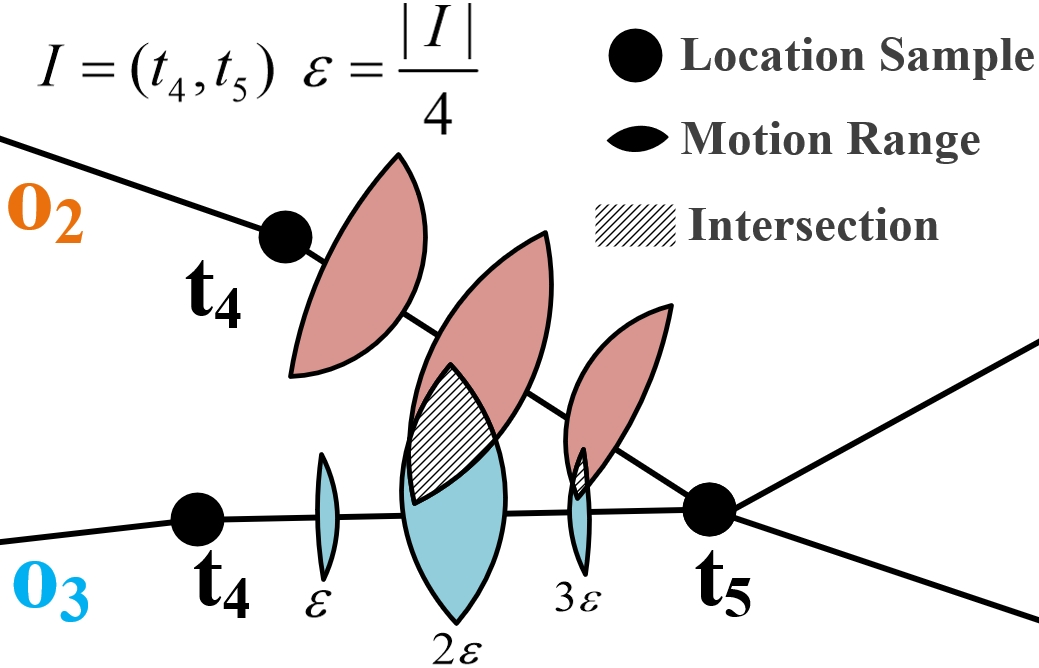
\includegraphics[width=0.6\columnwidth]{fig/section6/overall example.png}
    \caption{时间区间交集相似性的示意图}
    \label{fig:relaxed similarity example}
\end{figure}


我们在定义~\ref{defi:Tb-IS-Join} 中对交集相似性连接问题进行形式化描述。
\begin{definition}[IS-Join]\label{defi:Tb-IS-Join}
给定对象集合 $\mathcal{A}$ 和 $\mathcal{B}$、带有放宽划分参数 $\epsilon$ 的查询时间区间 $I$，以及相似性阈值 $\theta$，交集相似性连接（\underline{I}ntersection \underline{S}imilarity Join，IS-Join）旨在从这两个集合中找出所有交集相似性不小于 $\theta$ 的对象对所构成的集合 $\mathcal{P}$，即对于任意 $(o_i,o_j)\in (\mathcal{A}\times \mathcal{B})\setminus \mathcal{P}$，均有
$(IS(o_i,o_j,I,\epsilon)<\theta)$。
\end{definition}






\section{运动范围引导的匹配方法}

为高效地回答 IS-Join 查询，我们提出了一种由时间区间运动范围引导的匹配方法。在时间区间阶段，我们首先进行预检查，以判断两个对象的时间点运动范围之间是否存在交集。具体而言，我们定义时间区间运动范围 $MR(o,I)$，用于刻画对象 $o$ 在区间 $I$ 内可能到达的所有位置。如果 $MR(o, I)\cap MR(o', I)=\emptyset$，则可推出 $IS(o,o',I,\epsilon)=0$，从而对对象对 $(o,o')$ 进行剪枝。为高效判定 $MR(o,I)\cap MR(o',I)=\emptyset$，我们提出了一种新的混合 Ball-tree（Hybrid Ball-tree，HBall-tree）结构。同时，我们引入了一种基于交集相似度上界的剪枝增强方法，以进一步剔除不满足条件的对象对，从而细化整体处理流程。在精化阶段，计算运动范围内特征的交集以度量交集相似度。我们首先介绍基于时间区间运动范围的预检查策略，随后给出基于混合 Ball-tree 的连接算法（HBJ-Join）。

\subsection{时间区间预检查}\label{sec:inter pre-check}

本节介绍时间区间运动范围的概念，并给出具有理论保证的预检查策略。

\begin{definition}[时间区间运动范围]\label{defi:interval motion}
给定移动对象 $o$ 的两个带时间戳的位置样本 $s_i = ([x_i, y_i], t_i)$ 和 $s_{j}=([x_j,y_j], t_j)$，以及在 $t_i$ 与 $t_j$ 之间的最大速度 $v_{max}$，对象 $o$ 在时间区间 $I=[t_i,t_j]$ 内的运动范围，记为 $MR(o,I)$，被定义为对象 $o$ 在区间 $I$ 内可能到达的空间区域。
\end{definition}

定理~\ref{theorem:motion} 给出了计算 $MR(o,I)$ 的方法。

\begin{theorem}\label{theorem:motion}
对象 $o$ 的运动范围 $MR(o,I)$ 是由公式~\ref{eq:ellipse} 表示的一个椭圆区域。椭圆的中心点记为 $(x_c, y_c)$，由公式~\ref{eq:center} 计算得到；椭圆的旋转角度记为 $\alpha$，由公式~\ref{eq:angle} 计算，其中 $a$ 和 $b$ 分别表示半长轴和半短轴。
\begin{equation}
    \label{eq:ellipse}
    \begin{aligned}
 \left[\frac{(x-x_c)\cos\alpha+(y-y_c)\sin\alpha}{a}\right]^2+\\
    \left[\frac{(x_c-x)\sin\alpha+(y-y_c)\cos\alpha}{b}\right]^2 = 1
    \end{aligned}
\end{equation}
\begin{equation}
    \label{eq:center}
    \begin{aligned}
    x_c = \frac{x_i+x_{j}}{2}, \quad y_c=\frac{y_i+y_{j}}{2},\\
    a = \frac{v_{max}\cdot (t_{j}-t_i)}{2}, \\
    b=\frac{\sqrt{v_{max}^2\cdot (t_{j}-t_i)^2-(x_{j}-x_i)^2-(y_{j}-y_i)^2}}{2}
    \end{aligned}
\end{equation}
\begin{equation}
\label{eq:angle}
    \alpha = \arctan\!\left(\frac{y_{j}-y_i}{x_{j}-x_i}\right)
\end{equation}
\end{theorem}

\begin{proof} 
对象 $o$ 在时间区间 $I$ 内能够行进的最大距离为 $(t_j-t_i)\cdot v_{max}$，该结论同时适用于欧氏空间和路网空间。给定两个位置样本 $s_i$ 和 $s_j$，对象 $o$ 在某一具体时间点 $t$ 的运动范围可由公式~\ref{eq:timestamped motion range} 定义。需要注意的是，椭圆上任意一点到其两个焦点的距离之和为常数 $2a$。当 $v_{max}\cdot (t_j-t_i)=2a$ 时，从 $t_i$ 到 $t_j$ 的所有可能到达位置构成一个以 $(x_i, y_i)$ 和 $(x_j, y_j)$ 为焦点的椭圆区域，如图~\ref{fig:ellipse} 所示。我们对时间区间运动范围的建模方式与已有研究保持一致~\cite{DBLP:conf/edbt/ZhangRSL21,trajcevski2010uncertain}。
\end{proof}

\begin{figure}[tbp]
    \centering
    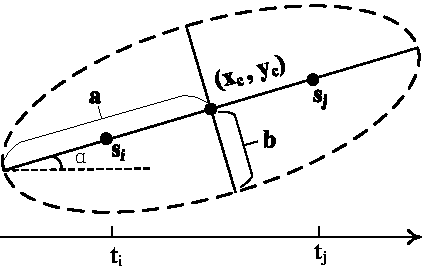
\includegraphics[width=0.6\columnwidth]{fig/section6/ellipse.pdf}
    \caption{时间区间运动范围示例}
    \label{fig:ellipse}
\end{figure}

基于定理~\ref{theorem:pre-checking}，我们提出了一种预检查策略：若 $MR(o,I)\cap MR(o',I)=\emptyset$，则可以在早期阶段安全地剪枝对象对 $(o,o')$，从而避免对特征集合（例如 POI、运动范围面积等）进行不必要的交集计算。

\begin{theorem}\label{theorem:pre-checking}
给定两个对象 $o$ 和 $o'$，若 $MR(o,I)\cap MR(o',I)=\emptyset$，则 $IS(o,o',I,\epsilon)=0$。
\end{theorem}

\begin{proof}
对于对象 $o$ 和 $o'$，如果它们在时间区间 $I$ 内的时间区间运动范围不相交，则在 $I$ 内任意时间点上，$o$ 与 $o'$ 的时间点运动范围都不可能发生重叠。由于与各自时间点运动范围相关的特征集合 $P(o,t)$ 和 $P(o',t)$ 在整个区间 $I$ 内均不存在交集，因此在区间 $I$ 上的交集相似度为 0。
\end{proof}

为了判断两个时间区间运动范围是否相交，一种直接的方法是计算它们的两两距离。具体而言，若距离
$dist(MR(o,I),MR(o',I))$ 大于 $MR(o,I).a + MR(o',I).a$，则两个运动范围不相交。其中，
$dist(MR(o,I),MR(o',I))$ 表示 $MR(o,I)$ 与 $MR(o',I)$ 中心点之间的距离，$a$ 表示运动范围的半长轴。
这种直接方法在进行一对一比较时需要 $O(\mathcal{A}\times \mathcal{B})$ 的时间复杂度，计算代价较高。

\label{sec:ball-tree}
\begin{figure*}[htbp]
    \centering
    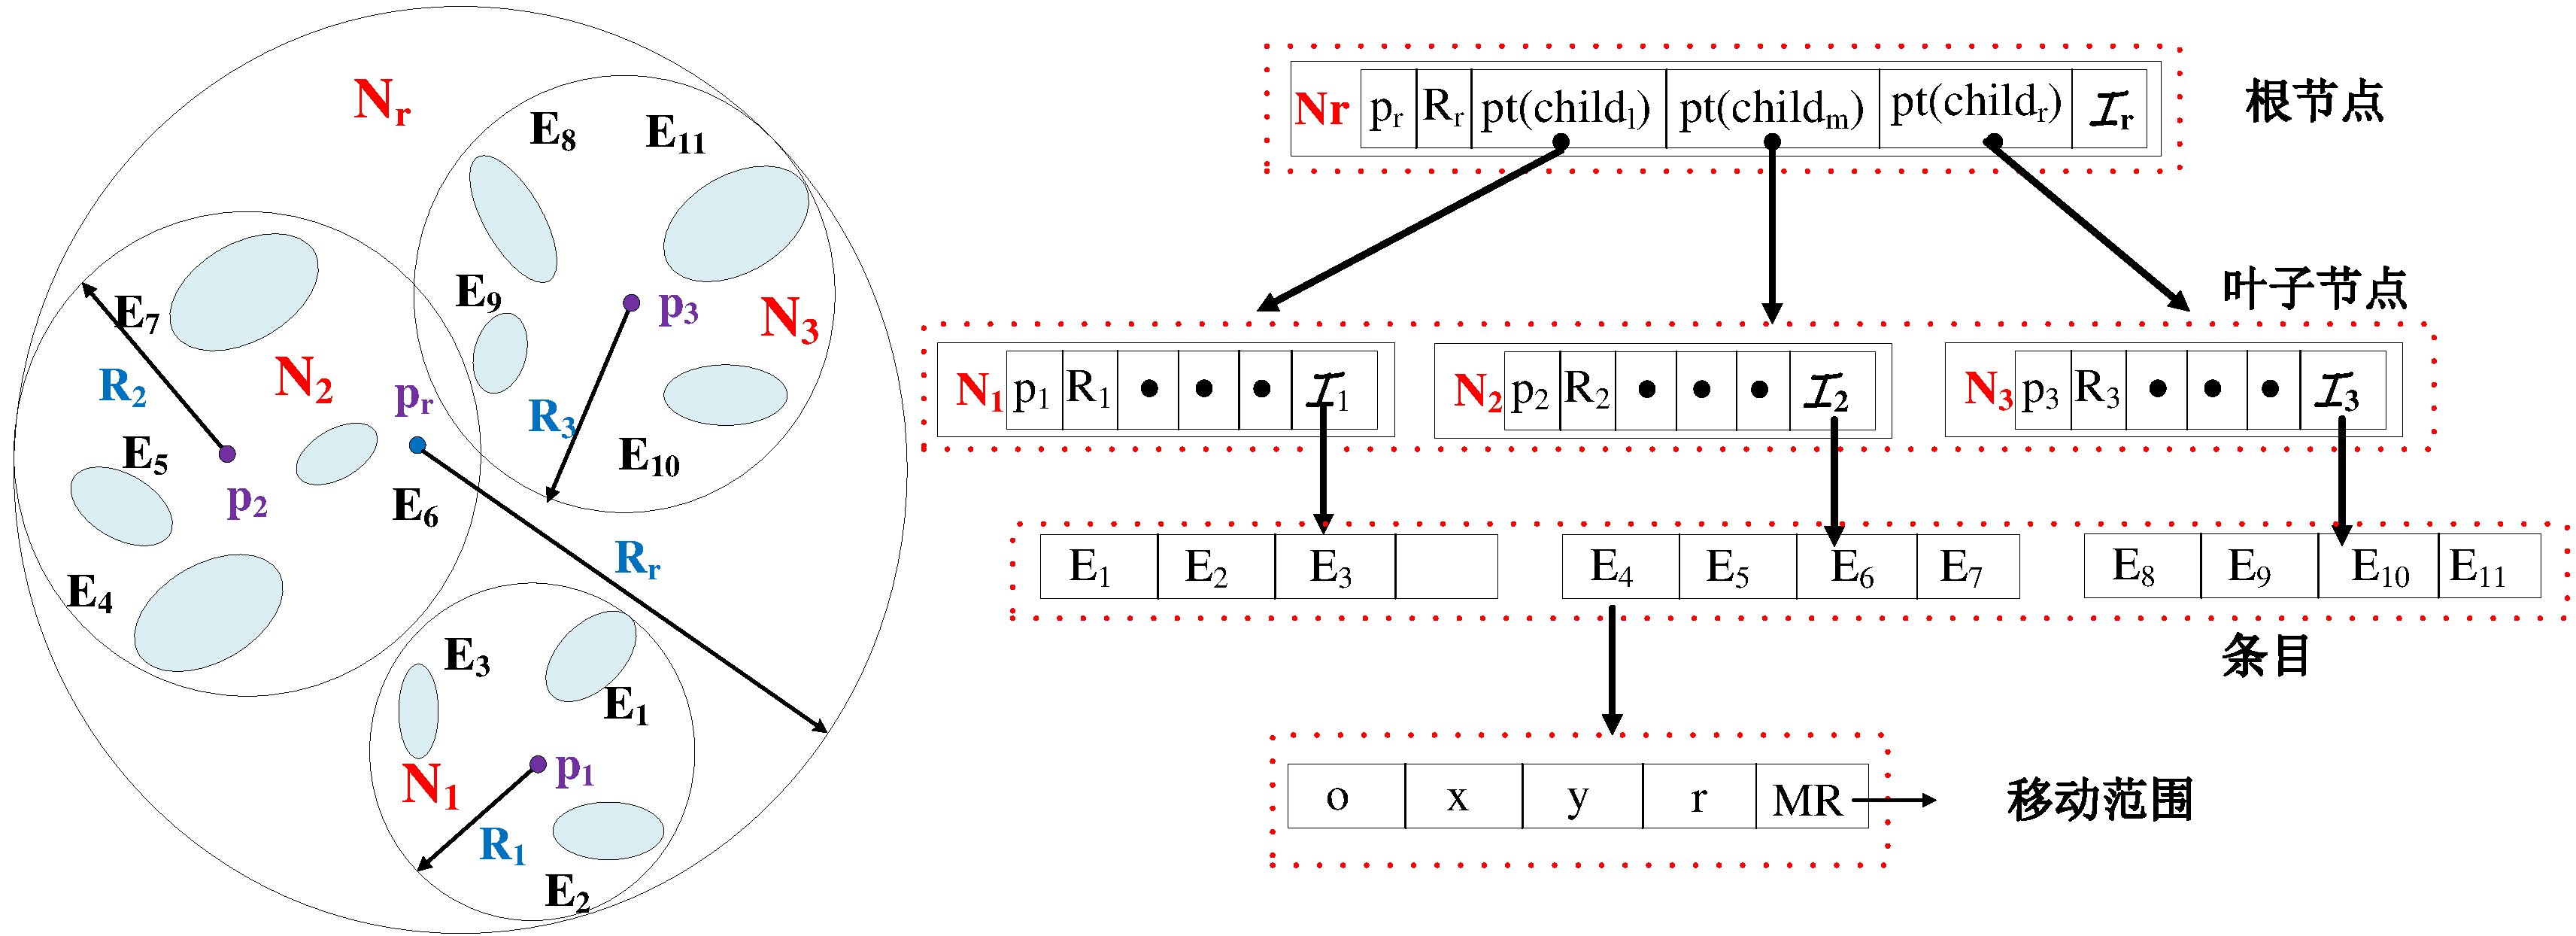
\includegraphics[width=1\textwidth]{fig/section6/ball-tree.pdf}
    \caption{混合 Ball-tree 的示意图}
    \label{fig:ball-tree}
\end{figure*}

```latex
\subsection{基于 HBall-tree 的交集预检查}
我们提出了一种混合 Ball-tree（Hybrid Ball-tree，HBall-tree），这是一种面向高效预检查的改进型索引结构，并展示了其如何提升“过滤–精化”过程的整体效率。

\subsubsection{HBall-tree}
\label{sec:hballtree}
我们选择 Ball-tree~\cite{omohundro1989five,DBLP:journals/jmlr/LiuMG06,DBLP:conf/uai/Moore00} 作为基础索引结构，这是因为相较于 R-tree~\cite{DBLP:conf/sigmod/Guttman84} 和四叉树~\cite{DBLP:journals/csur/Samet84} 等索引，Ball-tree 在处理类圆对象时表现更优~\cite{DBLP:conf/edbt/ZhangRSL21,DBLP:conf/sebd/CiacciaPRZ97,DBLP:conf/vldb/CiacciaPZ97}。然而，当将 Ball-tree 应用于 IS-Join 查询时，仍然存在两个关键局限性。首先，Ball-tree 主要面向点或圆级别的最近邻搜索设计，无法直接支持时间区间运动范围的索引。其次，其划分过程未考虑数据点的分布情况，可能导致划分不均衡，从而形成高度不平衡的树结构~\cite{DBLP:journals/corr/DolatshahHM15}。

为了解决第一个问题，我们将每个时间区间运动范围近似为一个圆~\cite{DBLP:conf/edbt/ZhangRSL21}。具体而言，该圆以时间区间运动范围的中心为圆心，其半径等于半长轴长度。该近似方式简化了时间区间运动范围的表示，使我们能够直接利用现有针对圆形对象设计的空间索引结构。其关键推论在于：如果两个近似圆不相交，则其对应的时间区间运动范围也必然不相交。该推论构成了我们过滤策略的基础，从而能够高效识别不可能发生交集的对象对。

为了解决第二个问题，我们提出了混合 Ball-tree（HBall-tree），这是一种能够考虑数据分布特性的全新索引结构。图~\ref{fig:ball-tree} 给出了 HBall-tree 的示意图。每个时间区间运动范围被表示为
$E=\{o,x,y,r,MR(o,I)\}$，
其中 $(x,y)$ 和 $r$ 分别表示近似圆的中心和半径，$o$ 表示对象标识符。与原始 Ball-tree 每个非叶节点仅包含两个子节点不同，HBall-tree 通过一种重新划分（repartition）技术，使得每个父节点最多可以拥有三个子节点。每个节点的结构表示为
$N=\{p,R,pt(child_l),pt(child_m),pt(child_r),\mathcal{I}\}$，
其中 $p$ 表示节点 $N$ 所覆盖的时间区间运动范围的中心点，$R$ 表示能够包围节点 $N$ 中所有条目（即圆）的半径，$pt(\cdot)$ 为指向子节点的指针，$\mathcal{I}$ 表示该节点中包含的时间区间运动范围集合。HBall-tree 中的插入策略、分裂策略以及枢轴点选择均遵循已有研究中的成熟方法~\cite{DBLP:conf/uai/Moore00}。当某一子划分中的对象数量低于预定义阈值（即生成新子节点所需的最小对象数）时，子划分过程终止。

\subsubsection{HBall-tree 的重新划分策略}
直观上，更加平衡的树结构通常能够在搜索过程中减少节点访问次数。重新划分方法的整体思想如下：对于每一个初始划分，我们评估其两个子划分中的点数差异是否超过重新划分阈值 $\beta$（$\beta \in (0,1)$）。如果差异超过该阈值，则保留点数较少的子划分，并将点数较多的子划分进一步划分为两个新的子划分。考虑一个节点 $N$，初始时 $N.child_m=\emptyset$。当较大的子划分规模至少以比例 $\beta$ 超过较小子划分时，即触发重新划分。例如，当 $|N.child_l.\mathcal{I}|>|N.child_r.\mathcal{I}|$，且
$\frac{|N.child_l.\mathcal{I}|-|N.child_r.\mathcal{I}|}{|N.child_r.\mathcal{I}|} \ge \beta$，
则触发重新划分。从理论上看，较小的重新划分阈值会使初始子树更容易被重新划分，从而增加三叉节点的数量，使树结构更加平衡。然而，三叉节点数量的增加也可能导致节点访问次数上升，因此需要在树高与三叉节点数量之间进行权衡。

对于非叶节点，初始划分基于 $N.\mathcal{I}$ 中选取的两个最远点进行。具体而言，树构建过程中两个最远点的选取步骤如下：(i) 随机种子点：从 $N.\mathcal{I}$ 中随机选择一个点作为初始种子；(ii) 第一个最远点：在数据集中找到距离该种子点最远的点；(iii) 第二个最远点：在数据集中找到距离第一个最远点最远的点。设这两个最远点分别为 $N.child_l.p$ 和 $N.child_r.p$，我们计算二者的中点，并在 $N.\mathcal{I}$ 中选取距离该中点最近的中心点，记为 $p_m$。点数较少的子划分被视为稳定划分，而我们对点数较多的子划分进行重新划分。具体地，若 $|N.child_l.\mathcal{I}|>|N.child_r.\mathcal{I}|$，则使用 $p_m$ 和 $N.child_l.p$ 将 $N.child_l.\mathcal{I}$ 中的运动范围重新划分为两个新的子划分，其中一个保留在 $N.child_l.\mathcal{I}$，另一个分配给 $N.child_m.\mathcal{I}$；反之，若 $|N.child_l.\mathcal{I}|<|N.child_r.\mathcal{I}|$，则使用 $p_m$ 和 $N.child_r.p$ 对 $N.child_r.\mathcal{I}$ 进行重新划分，一个子划分保留在 $N.child_r.\mathcal{I}$，另一个分配给 $N.child_m.\mathcal{I}$。最终，重新划分将原有的两个子划分扩展为三个子划分，新生成的子划分由 $N.pt(child_m)$ 索引。该重新划分技术带来了两方面优势：（1）降低树高与划分数量：通过提升平衡性，减少树的高度并最小化划分数量；（2）提升搜索效率：更加平衡的树结构能够减少树节点访问次数，从而提高搜索效率。
```
\subsection{基于 HBall-tree 的 Join}
我们提出了一种基于 HBall-tree 的 Join 算法。为了进一步提升效率，我们引入了一种剪枝增强方法，利用交集相似度的上界来进一步剔除不满足条件的对象对，从而优化整体处理流程。

\subsubsection{剪枝增强策略}
由于运动范围交集形状的不规则性，直接计算两个特征集合 $\mathcal{F}(o,t)$ 与 $\mathcal{F}(o',t)$ 的交集并非易事。给定时间点 $t$，若 $MR(o,t)\cap MR(o',t)\neq \emptyset$，当其中一个对象的运动范围完全被另一个对象覆盖时，$IS(o,o',t)$ 取得其最大值。基于这一观察，公式~\ref{eq:t-IS-ub} 给出了 $IS(o,o',t)$ 的一个上界。将公式~\ref{eq:t-IS-ub} 代入公式~\ref{eq:relaxed similarity}，可得到公式~\ref{eq:I-IS-ub1}，用于估计 $IS(o,o',I,\epsilon)$ 的上界。若 $IS(o,o',I,\epsilon)_{ub}<\theta$，则可以安全地剪枝对象对 $(o,o')$。

    \begin{equation}
    \label{eq:t-IS-ub}
    IS(o,o',t)_{ub} = 
   \frac{\min(|\mathcal{F}(o,t)|,|\mathcal{F}(o',t)|)}{\max(|\mathcal{F}(o,t)|,|\mathcal{F}(o',t)|)}\ge IS(o,o',t)
\end{equation}

    \begin{equation}
    \label{eq:I-IS-ub1}
     IS(o,o',I,\epsilon)_{ub} = \frac{\sum_{i=1}^{m} IS(o,o',t_i^\epsilon)_{ub}}{m}
\end{equation}

\begin{algorithm}[!h]
    \caption{$HBJ(\mathcal{A},\mathcal{B},N_r,I,\epsilon,\beta,\theta)$}
    \label{alg:ball filter}
    
    \Input{
    两组移动对象，$\mathcal{A}$ 和 $\mathcal{B}$；\newline
    HBall-tree 的根节点 $N_r$；\newline
    时间间隔 $I$；\newline
    松弛参数 $\epsilon$；\newline
    重分区阈值 $\beta$；\newline
    交集相似度阈值 $\theta$。
    }
    \Output{
    IS-Join 结果，$\mathcal{R}$。
    }
    
    \textbf{初始化:} $\mathcal{R} \leftarrow \emptyset$；
    
    \For(\tcc*[f]{遍历所有移动对象}){$o \in \mathcal{A}$}{
        $\mathcal{L} \leftarrow \{N_r\}$；
    
        \While(\tcc*[f]{BFS 遍历 HBall-tree}){$\mathcal{L} \neq \emptyset$}{
            $N \leftarrow \mathcal{L}.pop()$；
    
            \If(\tcc*[f]{非叶子节点分支}){$N$ 是非叶子节点}{
                \For(\tcc*[f]{遍历子节点}){$N_c \in N.pt(child)$}{
                    \If{$dist(o, N_c) \leq N_c.R + o.r$}{
                        $\mathcal{L}.push(N_c)$；
                    }
                }
            }
            \Else(\tcc*[f]{叶子节点处理}){
                \For(\tcc*[f]{遍历叶子节点对象}){$E \in N.\mathcal{I}$}{
                    \If{$dist(o, E) > E.r + o.r$}{
                        $prune(o, E.o)$;\tcp*[f]{预检查策略}
                    }
                    \If{$IS(o, E.o, I, \epsilon)_{ub} < \theta$}{
                        $prune(o, E.o)$;\tcp*[f]{剪枝增强策略}
                    }
                    \If{$IS(o, E.o, I, \epsilon) \geq \theta$}{
                        $\mathcal{R} \leftarrow \{\mathcal{R}, (o, E.o)\}$;\tcp*[f]{精炼步骤}
                    }
                }
            }
        }
    }
    \textbf{return} $\mathcal{R}$；
    \end{algorithm}



\subsubsection{算法细节}
算法~\ref{alg:ball filter} 给出了基于 HBall-tree 的 Join 算法（HBJ-Alg）的伪代码。该算法的输入包括两个移动对象集合、HBall-tree 的根节点、重分区阈值以及交集相似度阈值；输出结果为交集对象对集合 $\mathcal{R}$。初始时，$\mathcal{R}$ 为空（第 1 行）。对于每一个 $o\in\mathcal{A}$，我们使用列表 $\mathcal{L}$ 存储可能与 $MR(o,I)$ 发生交集的候选节点，初始时 $\mathcal{L}$ 仅包含根节点 $N_r$（第 3 行）。HBall-tree 通过插入对象集合 $\mathcal{B}$ 的时间区间运动范围构建完成。

当 $\mathcal{L}$ 非空时，算法调用 $\mathcal{L}.pop()$ 取出一个节点 $N$（第 5 行）。随后，在“圆级别”执行基于 HBall-tree 的过滤，以识别潜在的交集候选（第 6--9 行）。具体而言，我们检索 HBall-tree 中满足 $dist(o,N_c)\leq R+r_q$ 的节点，从而判断 $MR(o,I)$ 与 $N_c$ 之间是否可能存在交集。若 $N$ 为非叶节点，则检查其子节点。对于每个子节点 $N_c$，若对象 $o$ 与 $N_c$ 的距离不大于二者半径之和，则将 $N_c$ 压入优先队列（第 8--9 行）。

若 $N$ 为叶节点，则遍历 $N.\mathcal{I}$ 中的所有条目。对于每个条目 $E$，计算 $(E.x,E.y)$ 与 $(MR(o,I).x_c,MR(o,I).y_c)$ 之间的欧氏距离 $dist(o,E)$。若 $dist(o,E)>E.r+o.r$，则可安全剪枝 $(o,E.o)$（第 12--13 行）。否则，继续执行进一步的剪枝操作，即剪枝增强策略（第 14--15 行）。仅对保留下来的对象对，才进行精确的交集相似度计算，即利用公式~\ref{eq: time-point intersection similarity} 计算多个时间点的交集相似度（第 16--17 行）。最终返回结果集合 $\mathcal{R}$（第 18 行）。

\subsubsection{时间复杂度}
HBall-tree 的构建时间复杂度为 $O(|\mathcal{B}|\times \log|\mathcal{B}|)$。预检查阶段的时间复杂度为 $O(|\mathcal{A}|\times\log|\mathcal{B}|)$。设 $\mathcal{C}'$ 为候选集合，则候选精化阶段的时间复杂度为 $O(|\mathcal{C}'|\times |I|/\epsilon\times p)$。因此，HBJ-Alg 的总体时间复杂度为
\[
O\big((|\mathcal{A}|+|\mathcal{B}|)\times\log|\mathcal{B}| + |\mathcal{C}'|\times |I|/\epsilon\times p\big).
\]
HBJ-Alg 得益于增强的剪枝策略，显著减少了需要进行精化计算的候选对象对数量。











\section{实验研究}

\subsection{实验设置}
\subsubsection{数据准备}
实验研究~\footnote{代码已开源：\url{https://github.com/likemelike/IS-Join}} 在两个真实世界的轨迹数据集上进行。第一个数据集 Geolife \cite{DBLP:conf/huc/ZhengLCXM08,DBLP:journals/debu/ZhengXM10} 包含来自 182 名用户、历时四年的 17,621 条轨迹，涵盖了多种户外移动行为，包括日常通勤以及购物、骑行等休闲活动。第二个数据集 Porto~\cite{DBLP:journals/tits/Moreira-MatiasGFMD13} 包含在葡萄牙波尔图市 19 个月内记录的超过 170 万条出租车轨迹。Porto 数据集的轨迹以 15 秒为采样间隔记录，而 Geolife 的采样频率则不固定。时间戳被限定在 24 小时范围内，而不考虑具体日期，因为大多数城市交通出行行为具有日常重复性。我们将对象的最大速度 $v_{max}$ 定义为其在给定时间区间内观测到的最高速度。确定 $v_{max}$ 的真实取值或最优设置超出了本文的研究范围。为保证实际应用相关性，我们剔除了采样时间间隔过大（超过一小时）的极端轨迹，因为这类轨迹在现实应用中实用性有限，因此不纳入本研究。我们注意到，在隧道等环境中 GPS 信号可能较弱甚至完全丢失，从而导致异常位置或较低的采样率。尽管对这类异常值进行显式建模超出了本文的研究范围，但我们的数据预处理流程通过基于经度、纬度、轨迹长度和速度等约束过滤异常轨迹，从而在一定程度上缓解了这些影响。预处理后，Geolife 数据集中保留了 18,670 条轨迹中的 12,015 条有效轨迹，Porto 数据集中保留了 1,710,670 条轨迹中的 1,392,385 条。随后，从数据集中随机选取两个包含相同数量移动对象的对象组。

\subsubsection{对比算法}
我们将所提出的方法与一种设计良好的基于 M-tree 的连接算法~\cite{DBLP:conf/edbt/ZhangRSL21}（见附录）进行对比，记为 MBJ-Alg，作为基线方法。为评估剪枝增强策略的影响，我们还测试了不包含剪枝增强策略的 HBJ-Alg，记为 HBJ-Alg\#。在效率评估方面，我们同时衡量剪枝率和 CPU 时间。剪枝率定义为 $1- |C|/|O|^2$，其中 $C$ 表示候选集。CPU 时间表示算法每一轮的平均运行时间。此外，我们还评估了不采用重新划分策略的 HBJ-Alg，记为 HBJ-Alg$*$。

\begin{table}[tb]
	\centering
    \begin{tabular}{l|rr}
	\toprule
    \hline
		&\textbf{Geolife}&\textbf{Porto}\\
	\hline
        $|O|$ & \{4,6,8,10,12\} $\times 10^3$ & \{1,2,3,4,5\} $\times 10^4$  \\ 
        & 8K (默认) & 10K (默认) \\
    \hline
        $|I|$ & \{10s, 20s, 30s, 40s, 50s\}  & \{15s,  30s, 45s, 60s, 75s\} \\
		   & 30s (默认) & 45s (默认) \\
      \hline
        $|\mathcal{F}|$ & \{2, 4, 6, 8, 10\}$\times 10^5$  & \{1, 2, 3, 4, 5\}$\times 10^5$  \\
		   & 600K (默认) & 100K (默认) \\
     \hline
        $\epsilon$ & \{$\frac{|I|}{2}$,   $\frac{|I|}{4}$, $\frac{|I|}{6}$, $\frac{|I|}{8}$, $\frac{|I|}{10}$\}   & \{$\frac{|I|}{2}$,   $\frac{|I|}{4}$, $\frac{|I|}{6}$, $\frac{|I|}{8}$, $\frac{|I|}{10}$\}  \\
		   & $\frac{|I|}{6}$ (默认) & $\frac{|I|}{6}$ (默认) \\
\bottomrule
    \end{tabular}
    \caption{评估参数设置}
    \label{tb:algorithm_para}
\end{table}

\subsubsection{参数设置}
参数设置如表~\ref{tb:algorithm_para} 所示。M$^\ast$-tree 和 HBall-tree 的叶节点容量均设置为 10。默认情况下，重新划分阈值 $\alpha$ 设为 0.5。在实验中，特征集合 $\mathcal{F}$ 由随机生成的兴趣点（POIs）构成。具体而言，我们首先确定所有轨迹的最小和最大经度与纬度值，在该空间范围内使用均匀分布随机生成固定数量的 POIs。默认情况下，在 Porto 数据集的坐标范围内生成 100,000 个 POIs，在 Geolife 数据集中生成 600,000 个 POIs。默认距离度量采用欧氏距离。所有方法均使用 Java 实现，并在配备 AMD Ryzen 5 CPU（3.6GHz）和 32GB 内存的 Ubuntu 系统上进行评测，采用单线程执行。除非另有说明，实验结果均为 20 次独立实验的平均值，每次实验使用不同的轨迹数据和特征集。


\subsection{Performance Evaluation}

\subsubsection{剪枝有效性评估}
首先，我们在默认参数设置下考察各算法的剪枝有效性。实验结果如表~\ref{tb:prune} 所示。通过比较 MBJ-Alg 与 HBJ-Alg 的候选集规模和剪枝率可以发现，在 Geolife 和 Porto 数据集上，HBJ-Alg 的候选集规模分别仅为 MBJ-Alg 的 0.5\% 和 2.3\%。这些结果表明，所提出的方法能够显著压缩搜索空间。

\begin{table}[tb]
    \begin{tabular}{|p{6cm}|p{3cm}|p{3cm}|}
        \hline
        \diagbox{指标/数据集}{方法} & MBJ-Alg & HBJ-Alg  \\
        \hline
        候选集规模（Geolife） & 6540764 & 28862\\
        \hline
        剪枝率（Geolife） & 89.7800\% & 99.9549\%\\
        \hline
        候选集规模（Porto） & 2142988 & 50072\\
        \hline
        剪枝率（Porto） & 97.8570\% & 99.9499\%\\
        \hline
    \end{tabular}
    \caption{剪枝性能}
    \label{tb:prune}
\end{table}

接下来，我们在不同参数设置下进一步评估所提出算法的性能。需要说明的是，在改变某一个参数时，其余参数均保持为默认值。

\subsubsection{移动对象基数的影响}
我们研究了不同移动对象基数 $|O|$ 对算法性能的影响。直观上，较大的 $|O|$ 会导致需要处理更多的时间区间运动范围，因此所有算法的运行时间都将随之增加。首先，我们评估了 MBJ-Alg、HBJ-Alg 以及 HBJ-Alg$*$ 的索引构建时间，结果如图~\ref{img:vary_num_ctime} 所示。可以清楚地看到，MBJ-Alg 的构建开销明显高于 HBJ-Alg。与 HBJ-Alg$*$ 相比，HBJ-Alg 表现出相近且略有提升的性能。这一改进主要得益于 HBJ-Alg 中的再划分技术：尽管在触发再划分时会引入额外计算开销，但该技术能够减少总体分区数量，从而在整体上有助于降低构建时间。

接下来，我们分析了所提出算法在 IS-Join 查询中的总运行时间。随着移动对象数量的增加，由于交集候选对数量增多，计算负载显著上升，所有算法的时间复杂度均随之提高。从图~\ref{img:vary_num_ftime} 可以观察到，随着数据规模的扩大，MBJ-Alg 的 CPU 时间显著增加。例如，在 Geolife 数据集包含 12K 个移动对象、Porto 数据集包含 50K 个移动对象时，MBJ-Alg 的查询时间分别超过 3 秒和 30 秒，计算开销较大。相比之下，HBJ-Alg 和 HBJ-Alg\# 始终优于 MBJ-Alg，尤其在大规模数据集上表现出更高的效率。值得注意的是，HBJ-Alg 的 CPU 时间几乎没有明显退化，充分体现了所提出方法的良好可扩展性。此外，与 HBJ-Alg\# 相比，HBJ-Alg 的运行时间降低了约 30\%，突出了剪枝增强策略所带来的性能提升。具体而言，在 Geolife 数据集包含 12,000 个移动对象、Porto 数据集包含 50,000 个移动对象时，HBJ-Alg 相比 MBJ-Alg 在 Geolife 上实现了 $3.1x$ 的加速，在 Porto 上实现了 $3.3x$ 的加速。

\begin{figure}[tb]
    \centering
    \subfloat[]{
    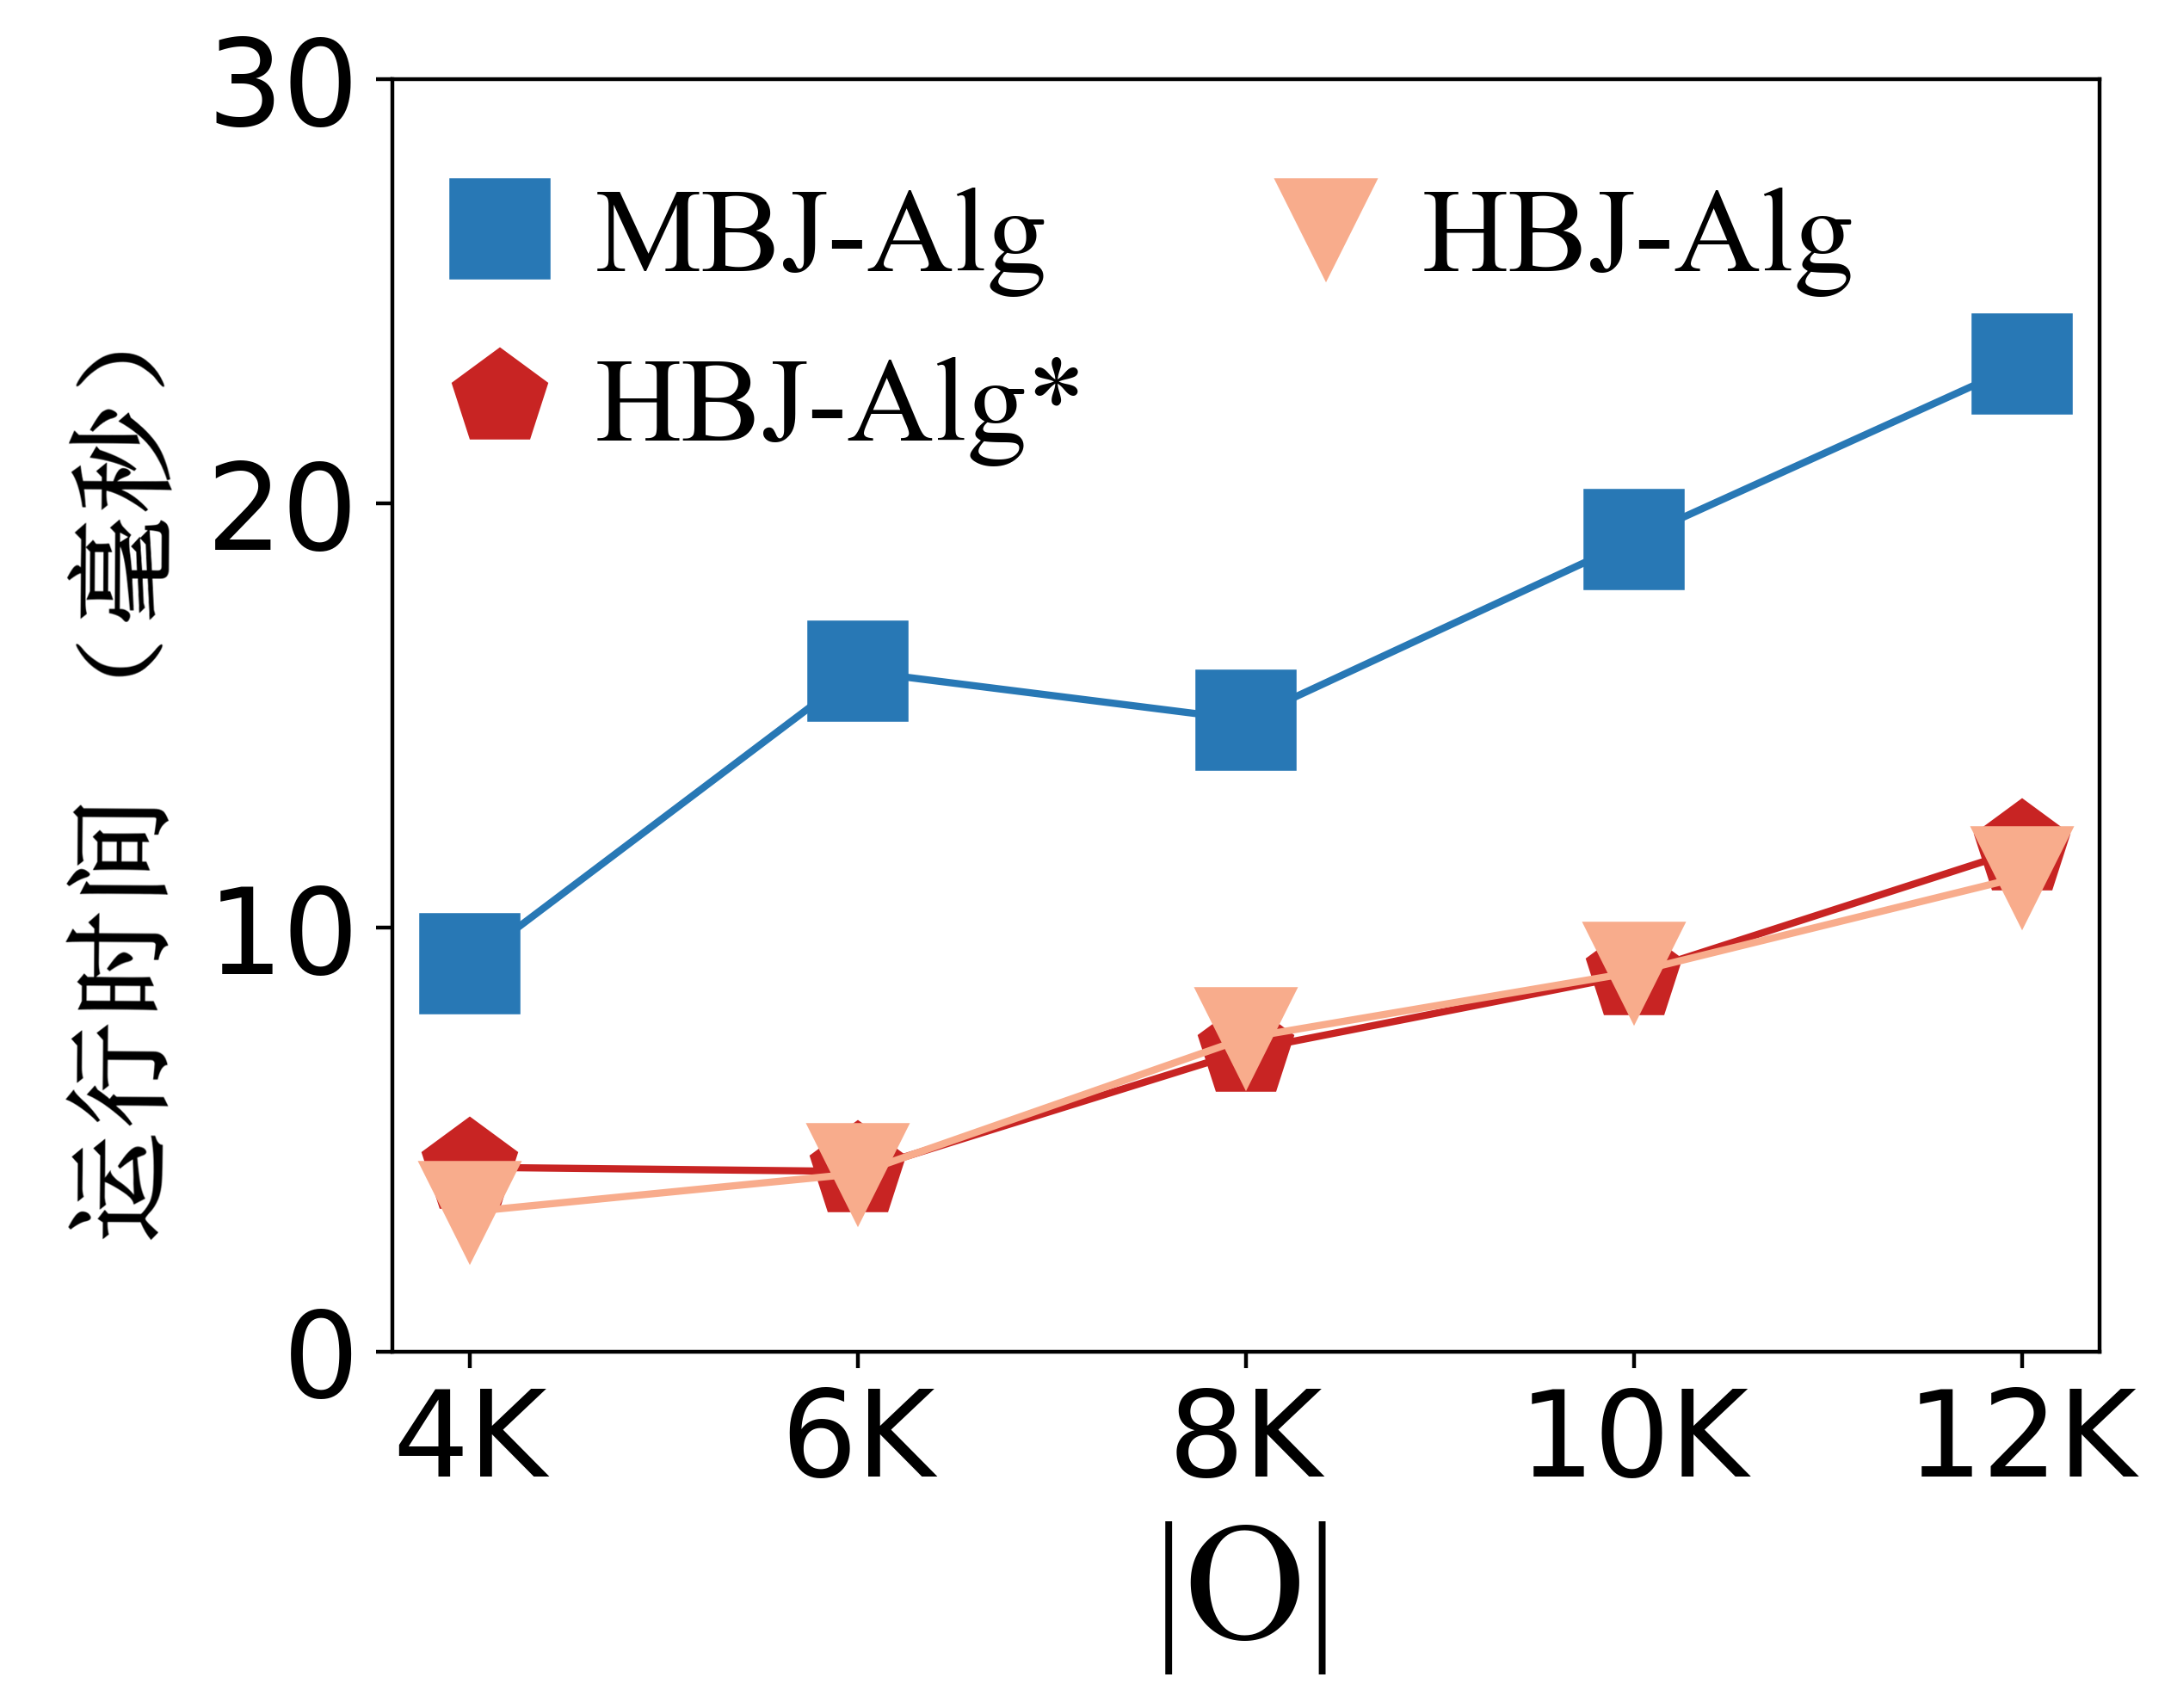
\includegraphics[width=0.5\textwidth]{fig/section6/geo-num-ctime.png}
    \label{geo-num-ctime}
}% 
\subfloat[]{
    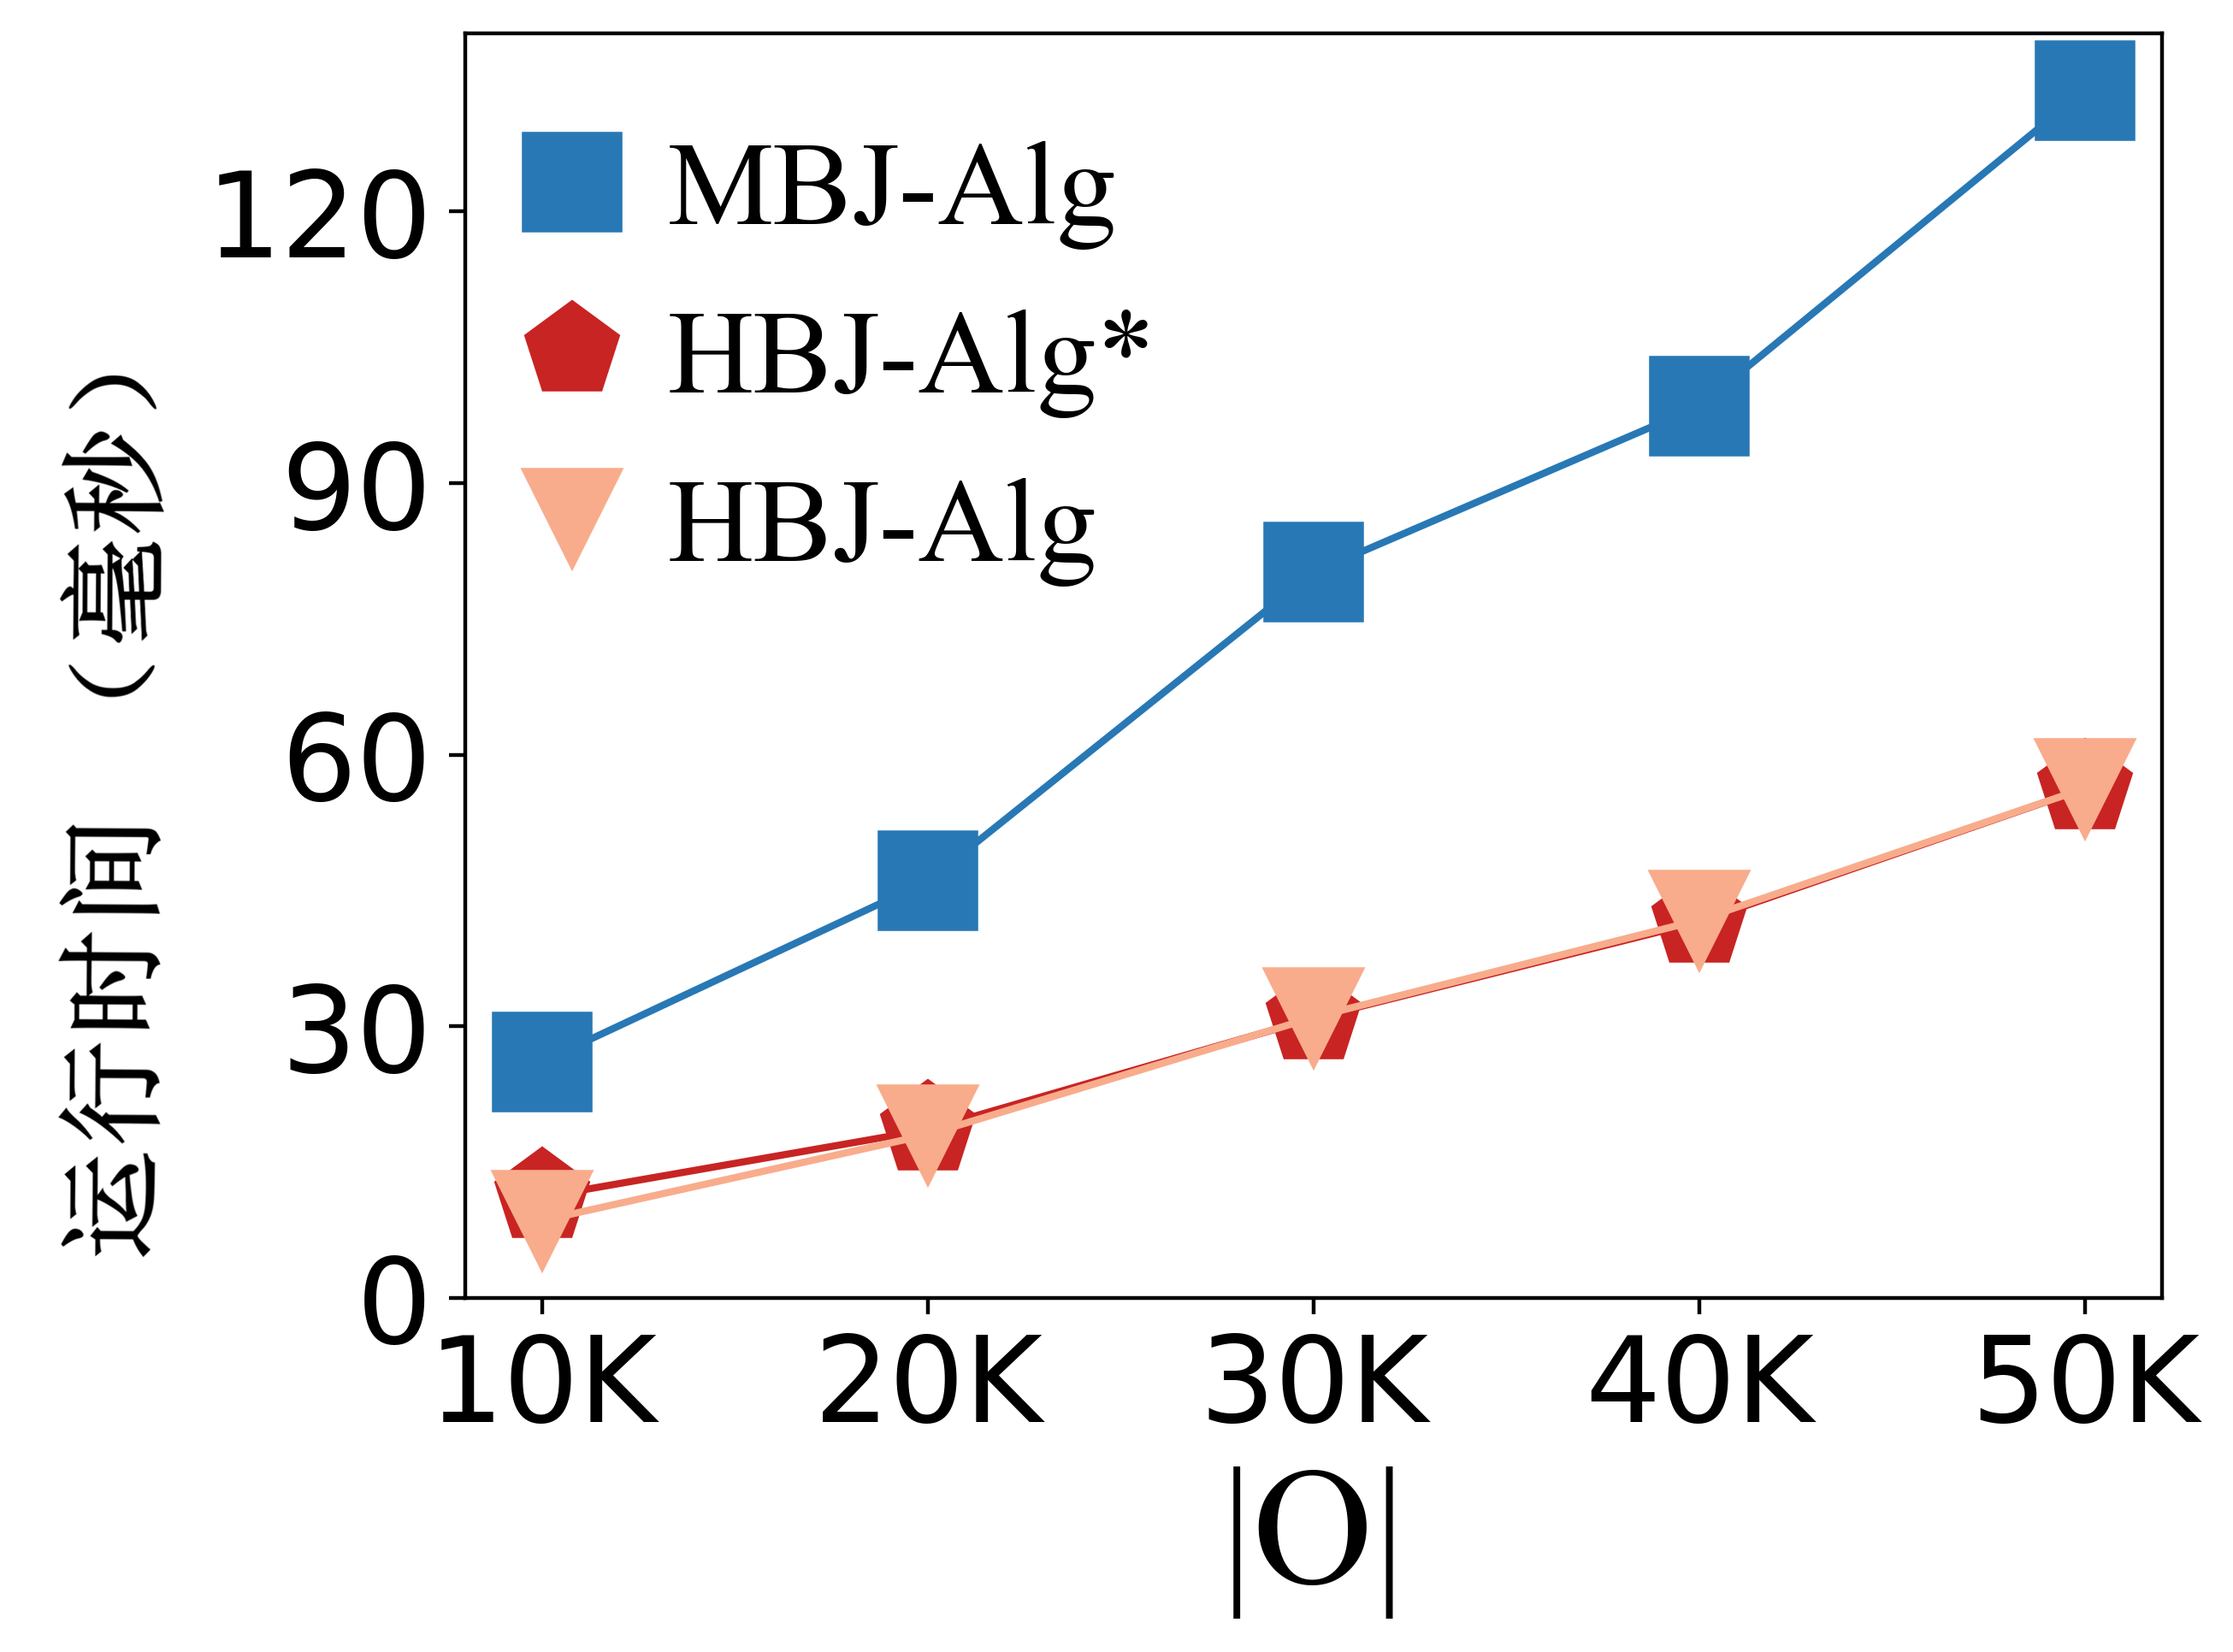
\includegraphics[width=0.5\textwidth]{fig/section6/pt-num-ctime.png}
    \label{pt-num-ctime}
}% 
\caption{不同 $|O|$ 下的构建时间影响 \subref{geo-num-ctime}:Geolife数据集下的实验; \subref{pt-num-ctime}:Porto数据集下的实验}
\label{img:vary_num_ctime}
\end{figure}

\begin{figure}[tb]
    \centering
    \subfloat[]{
    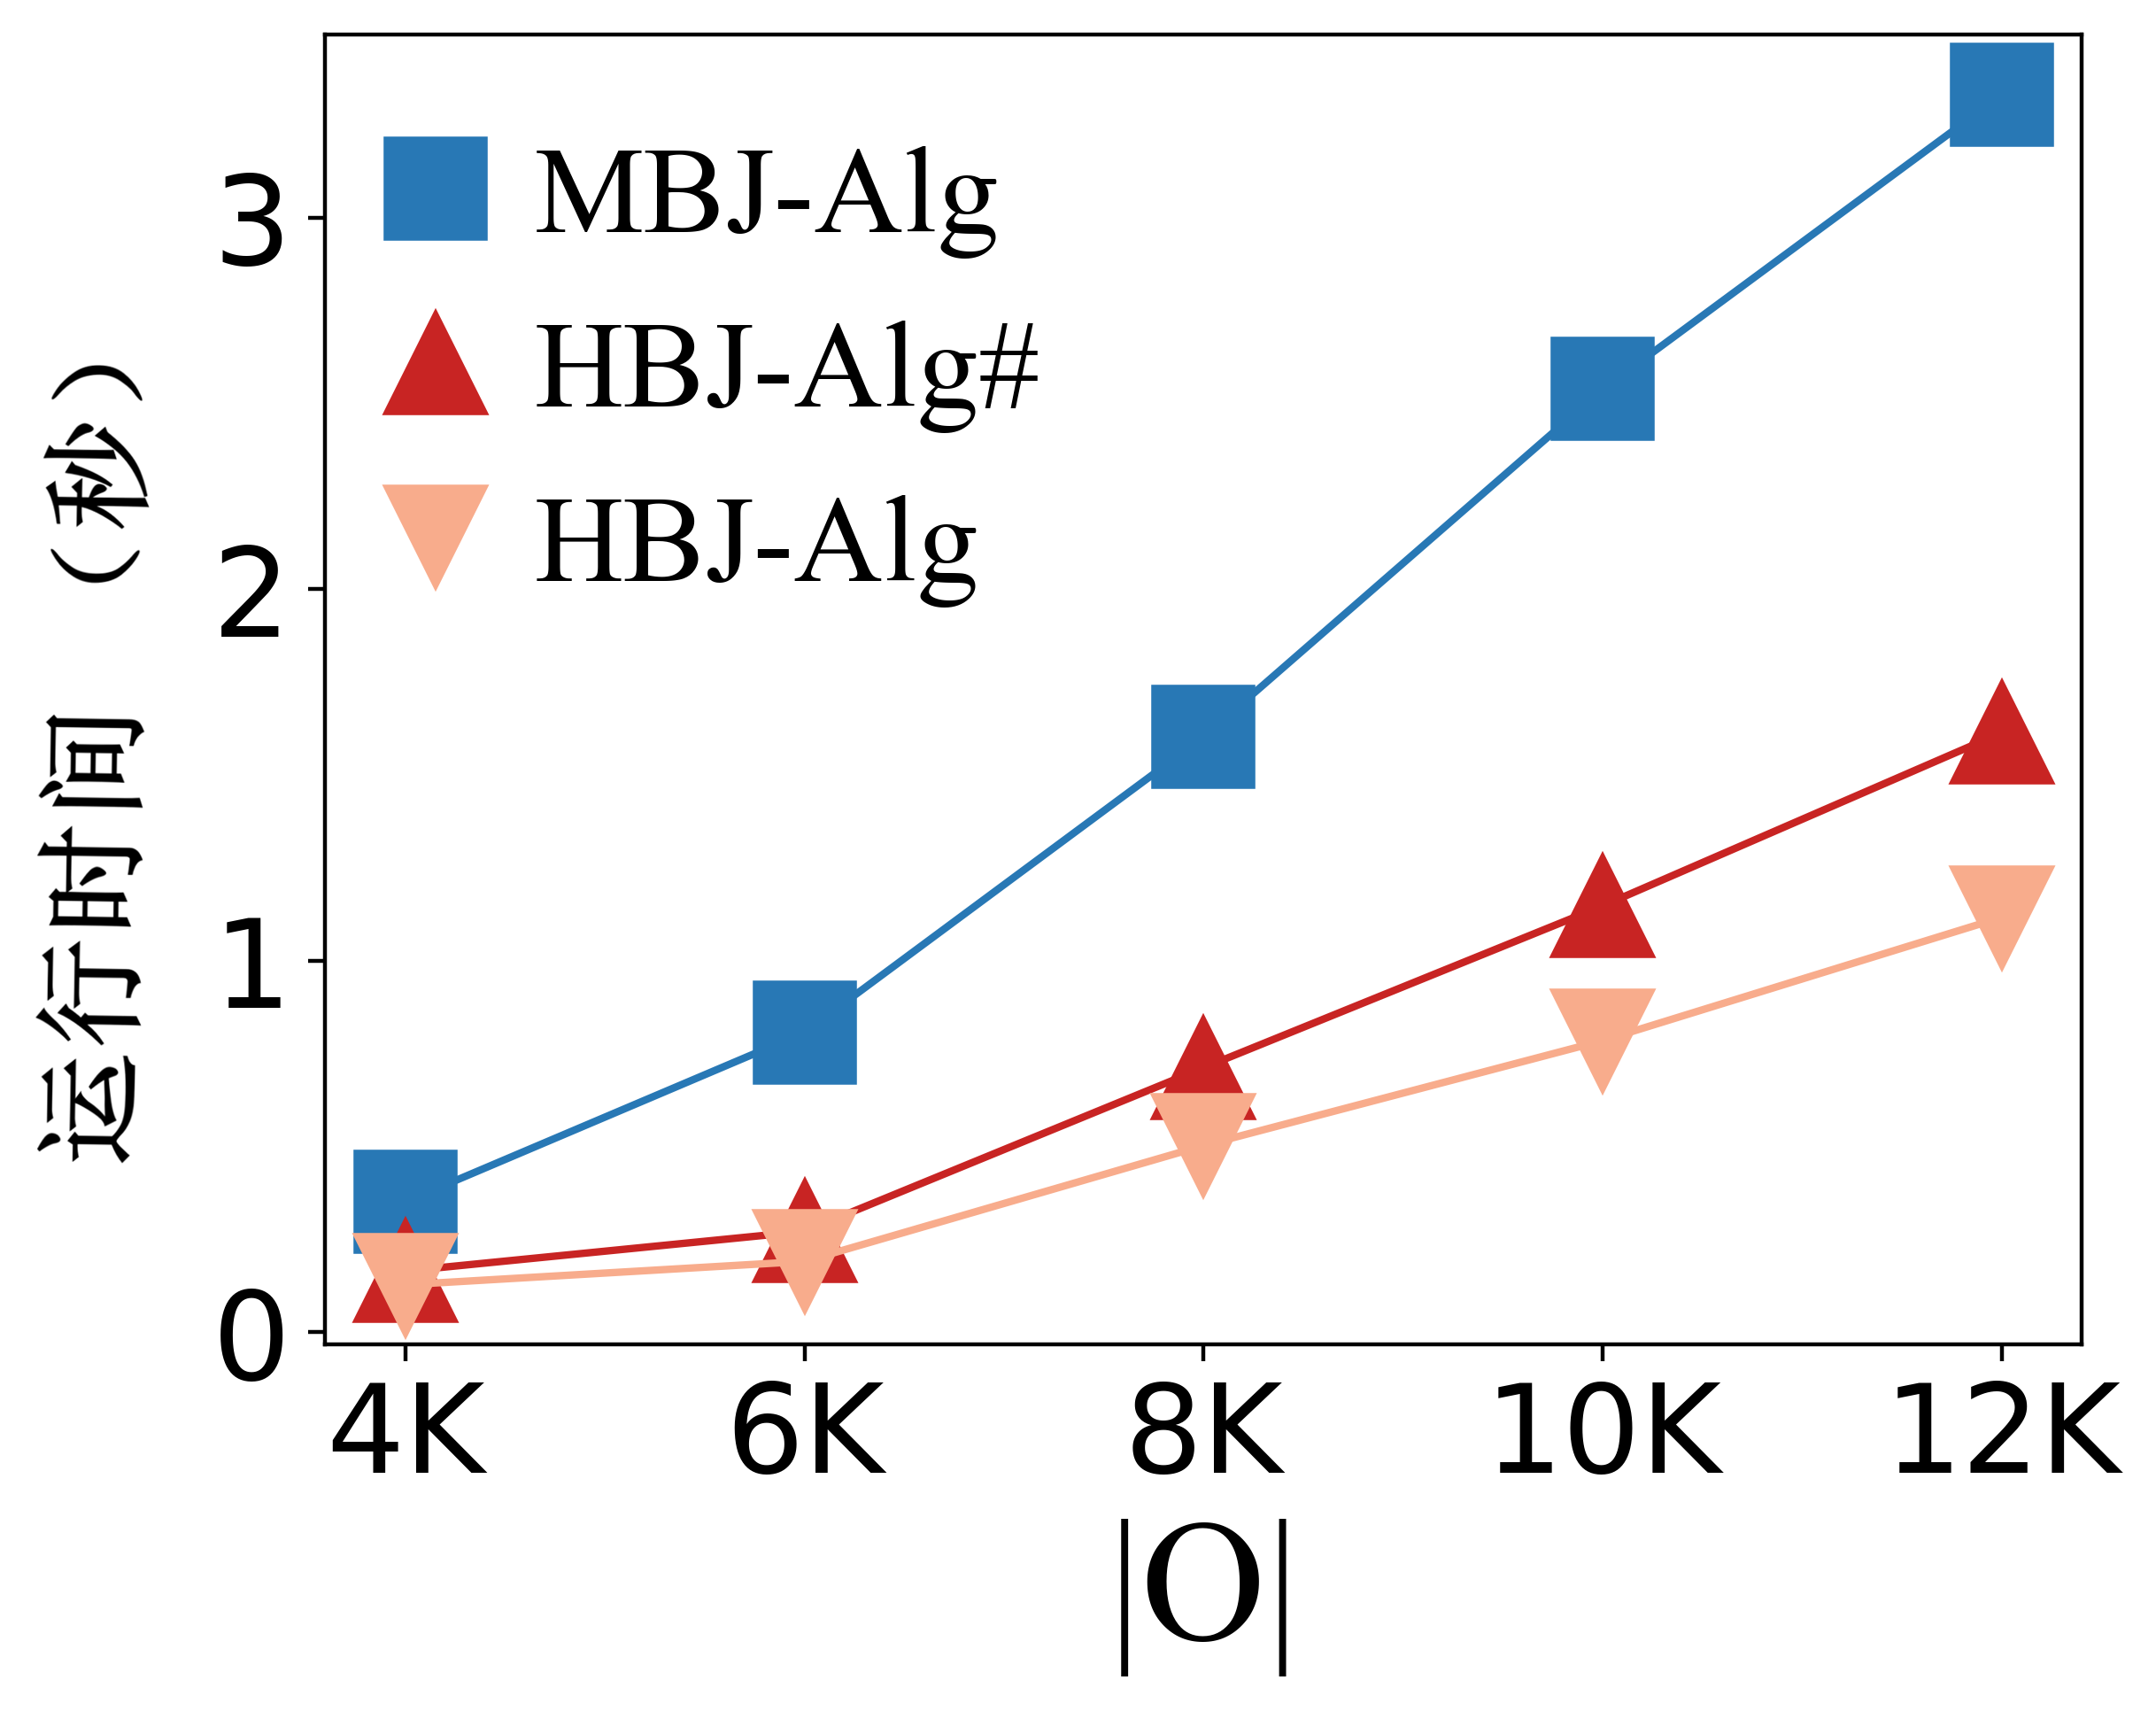
\includegraphics[width=0.5\textwidth]{fig/section6/geo-num-ftime.png}
    \label{geo-num-ftime}
}% 
\subfloat[]{
    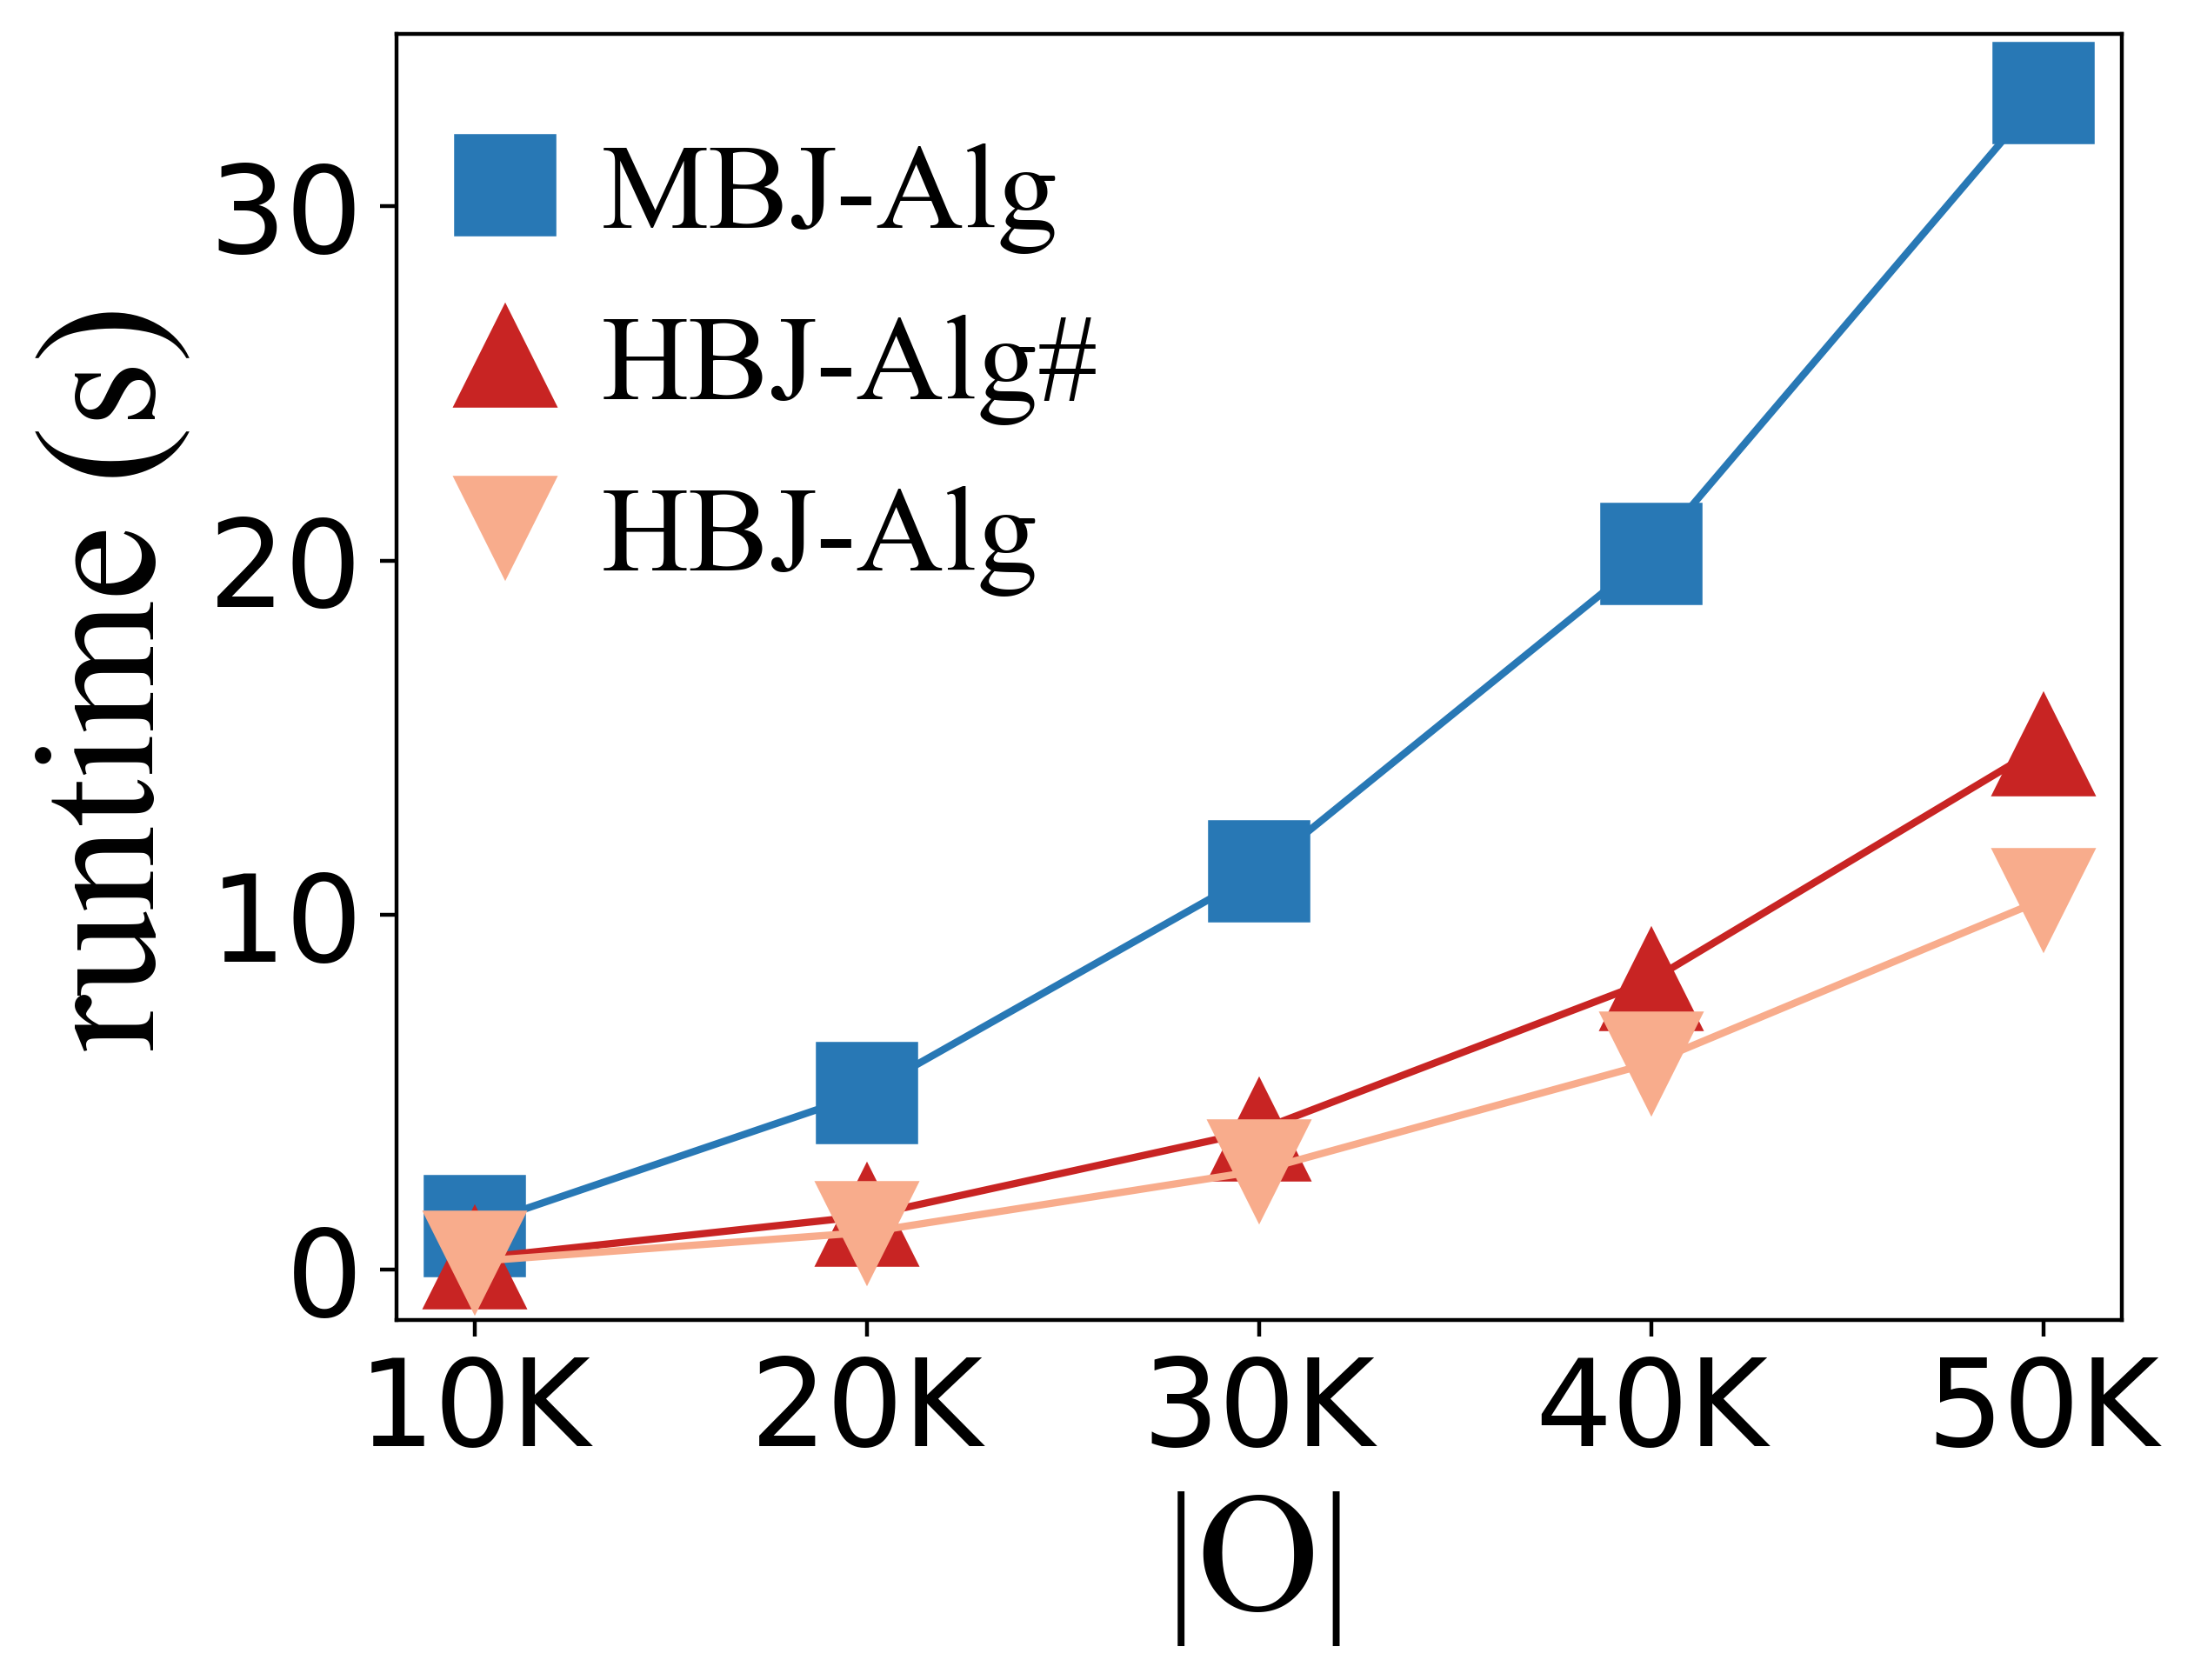
\includegraphics[width=0.5\textwidth]{fig/section6/pt-num-ftime.png}
    \label{pt-num-ftime}
}% 
\caption{不同 $|O|$ 下的查询时间影响 \subref{geo-num-ftime}:Geolife数据集下的实验; \subref{pt-num-ftime}:Porto数据集下的实验}
\label{img:vary_num_ftime}
\end{figure}

\subsubsection{特征数量的影响}
在实验中，我们将运动范围的特征集合设定为兴趣点（POI）。直观而言，在相同的时间区间运动范围内，较大的 $|\mathcal{F}|$ 意味着两个对象之间存在更多潜在的交集位置，这可能由于需要进行额外的位置检查而导致运行时间增加。如图~\ref{img:vary_poi_ftime} 所示，随着 $|\mathcal{F}|$ 的增大，所有算法的运行时间均呈现出轻微的上升趋势。然而，所提出的预检查策略和剪枝增强方法能够在早期阶段有效地剔除大量不可能满足条件的对象对，从而显著减少需要进行 POI 交集计算的候选数量。因此，POI 集合规模对整体运行时间的影响较小，进一步验证了所提出方法的良好可扩展性。

\begin{figure}[tb]
    \centering
    \subfloat[]{
    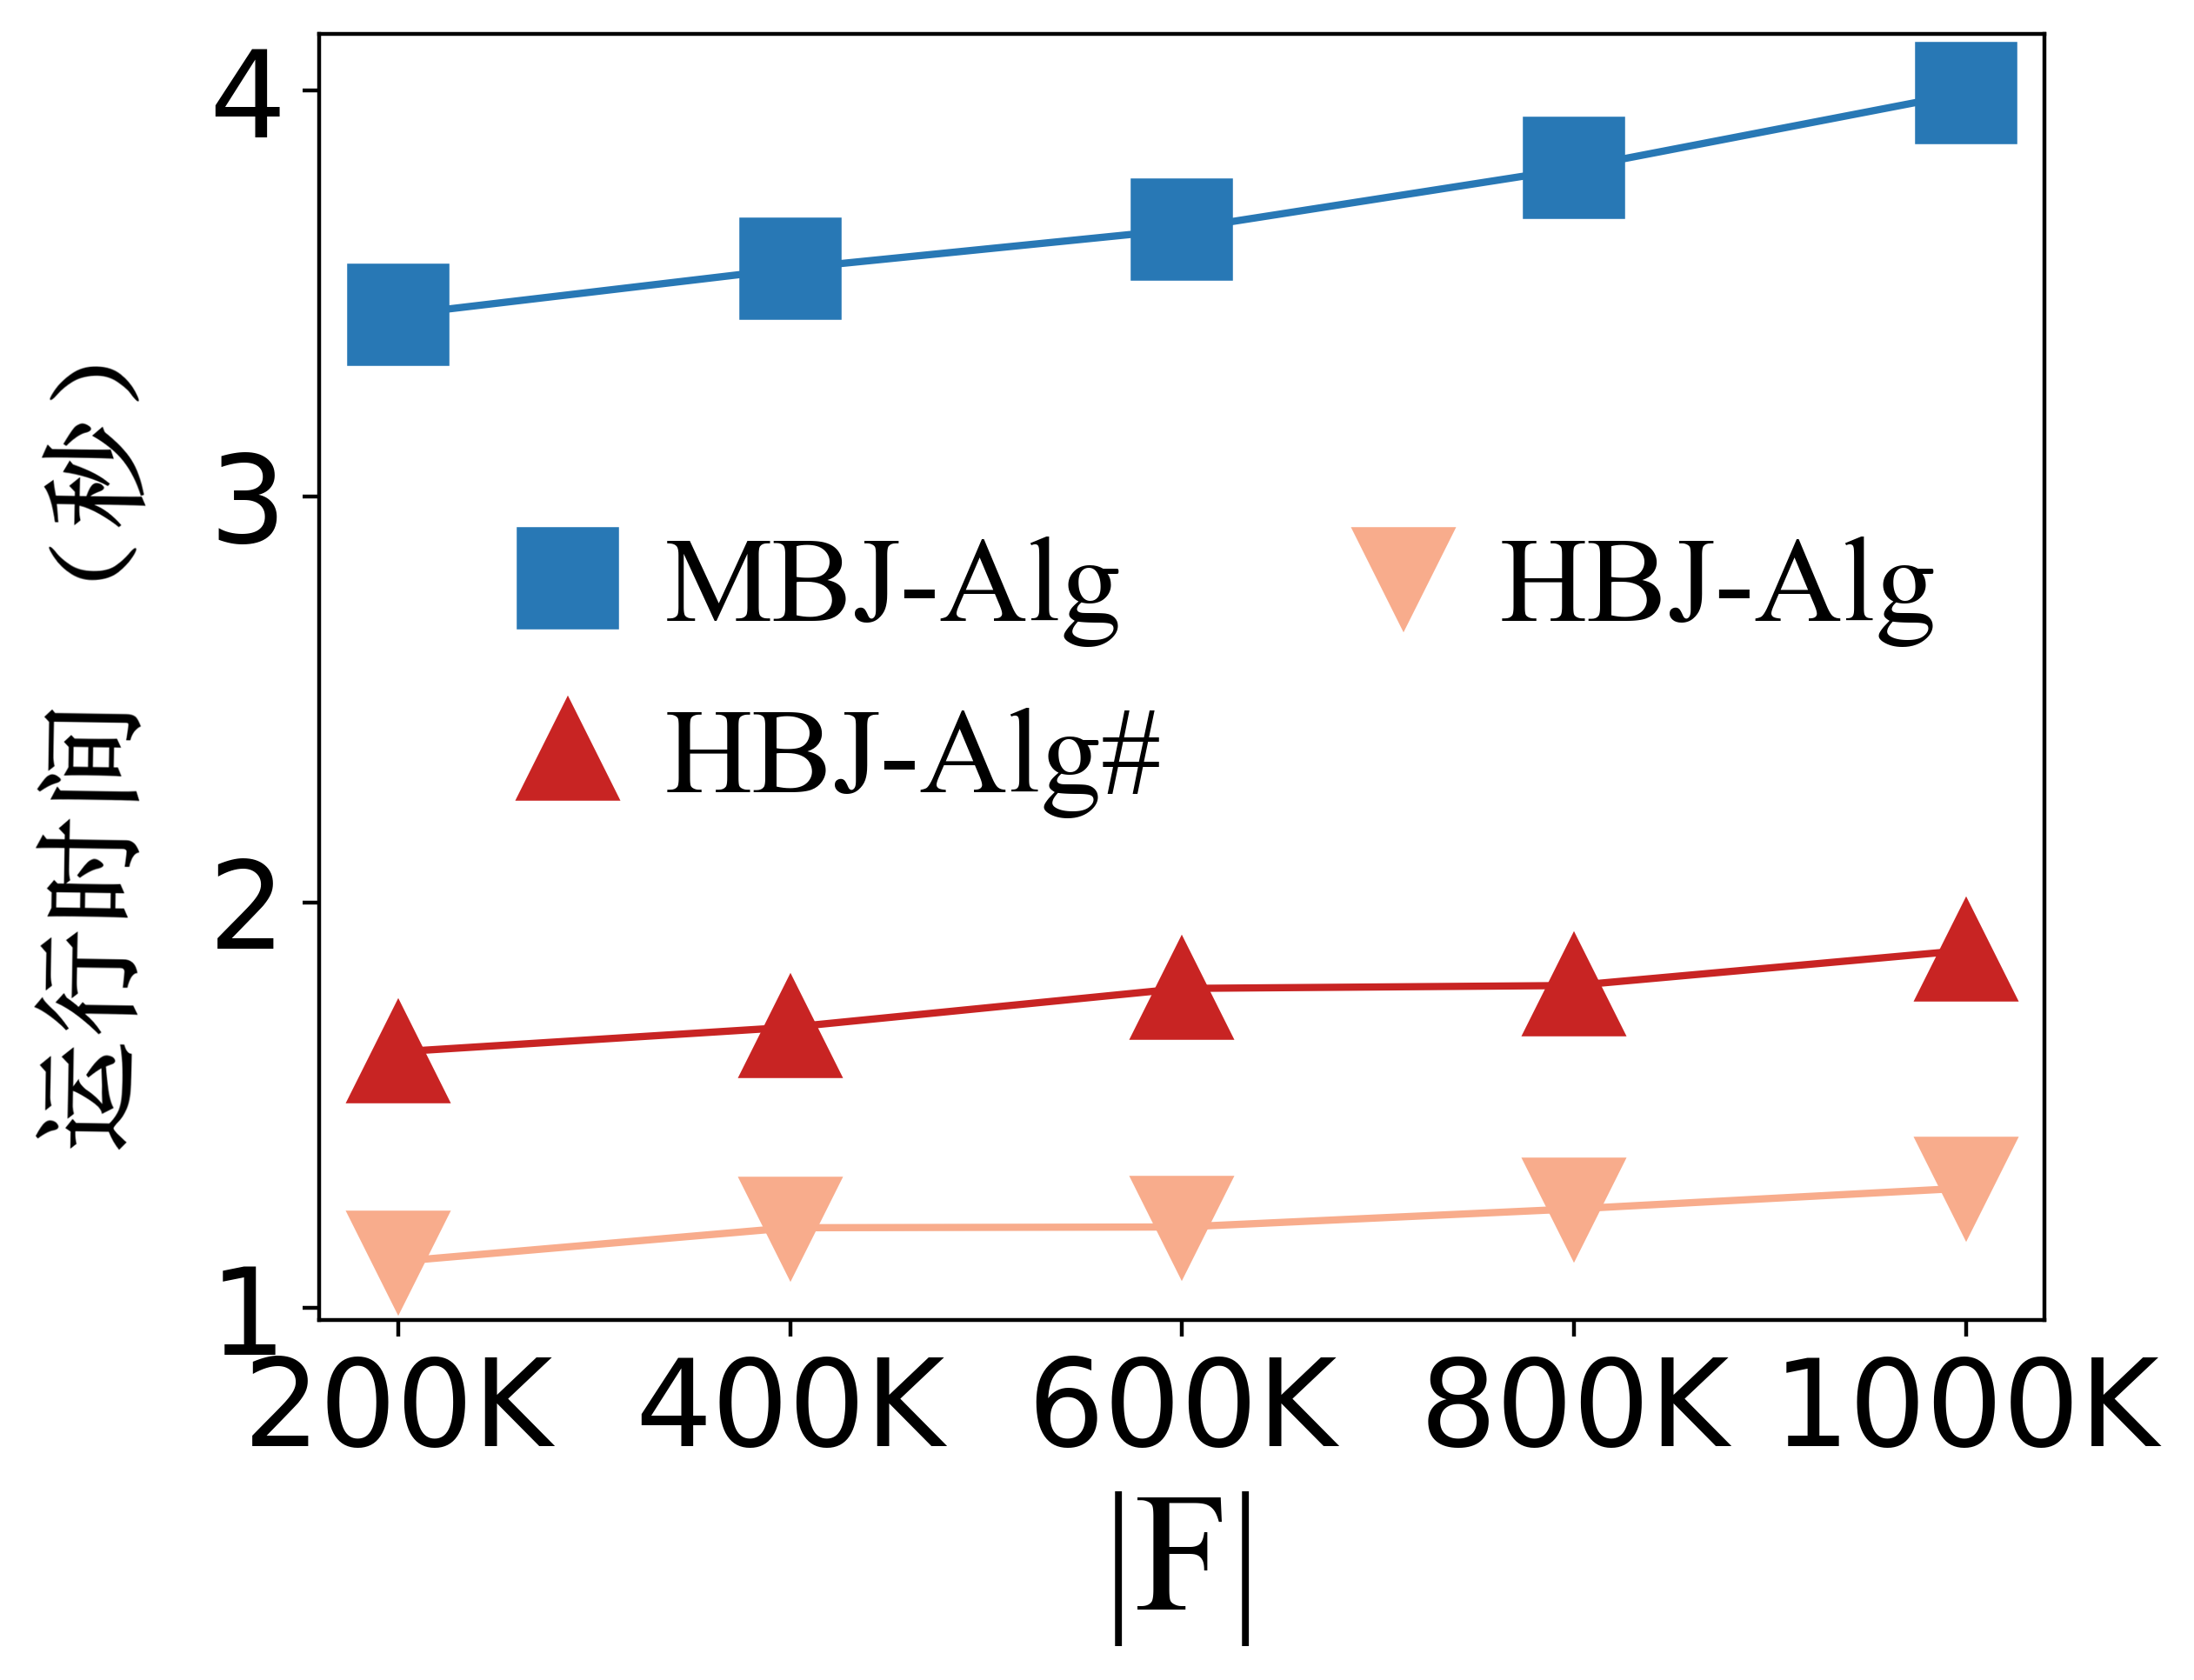
\includegraphics[width=0.5\textwidth]{fig/section6/geo-poi-ftime.png}
    \label{geo-poi-ftime}
}% 
 \subfloat[]{
    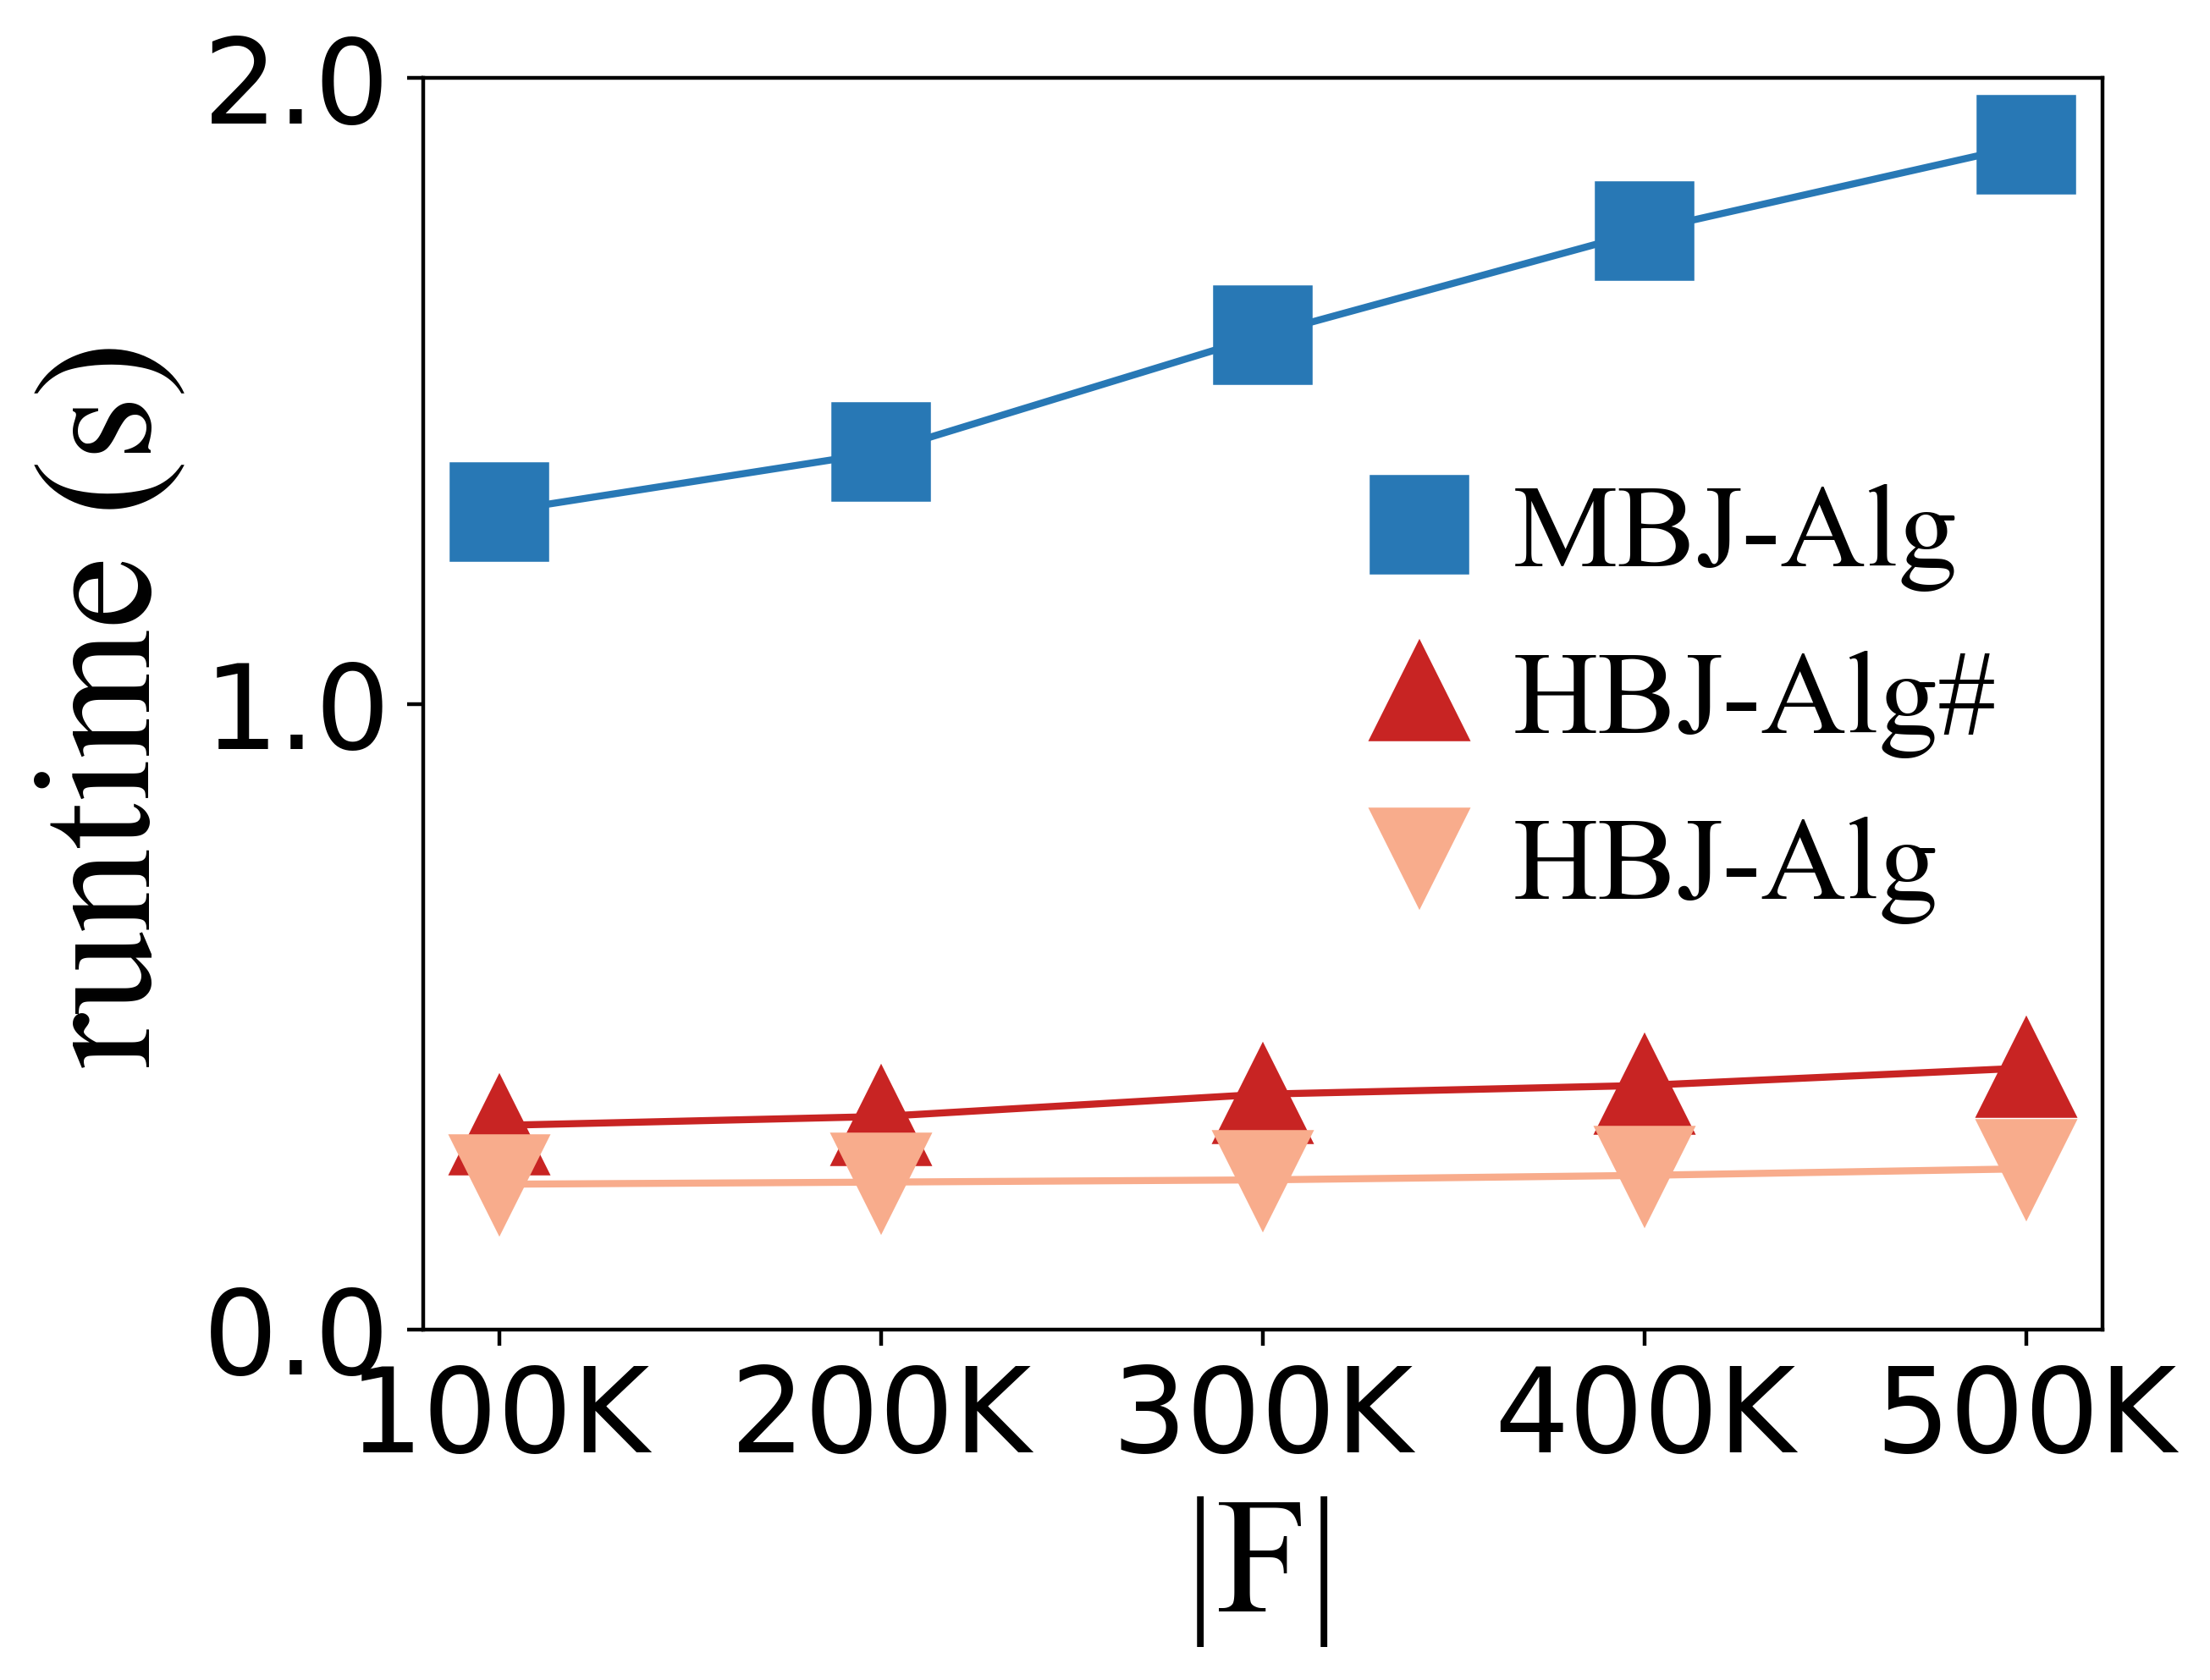
\includegraphics[width=0.5\textwidth]{fig/section6/pt-poi-ftime.png}
    \label{pt-poi-ftime}
}% 
\caption{POI 数量对运行时间的影响 \subref{geo-poi-ftime}:Geolife数据集下的实验; \subref{pt-poi-ftime}:Porto数据集下的实验}
\label{img:vary_poi_ftime}
\end{figure}

\subsubsection{时间区间的影响}
我们使用 $|I|$ 表示给定时间区间的持续时长。具体而言，在 Geolife 数据集中，$|I|$ 从 10 秒变化到 50 秒；在 Porto 数据集中，$|I|$ 从 15 秒变化到 75 秒。较大的 $|I|$ 会扩大潜在的时间区间运动范围，从而导致具有交集的对象对数量增加以及候选集规模增大。因此，所有算法在识别满足条件的对象对时都需要更多的计算开销。图~\ref{img:vary_I_ftime} 展示了随着 $|I|$ 增大时的效率表现。正如预期的那样，随着 $|I|$ 的增加，所有算法的运行时间均呈上升趋势，其中 HBJ-Alg 在所有参数设置下始终优于 MBJ-Alg 和 HBJ-Alg\#。通过利用 M*-tree，我们在一定程度上提升了过滤性能，并减少了后续需要进一步处理的候选对象数量。然而，由于 M-tree 的原始设计在构建阶段需要进行耗时的节点分裂操作，其并不适合直接用于 IS-Join 查询。此外，在大规模移动对象场景下，对仅覆盖单个时间区间运动范围的圆进行索引，可能会导致搜索空间膨胀，从而对查询性能产生不利影响。

\begin{figure}[tb]
    \centering
    \subfloat[]{
    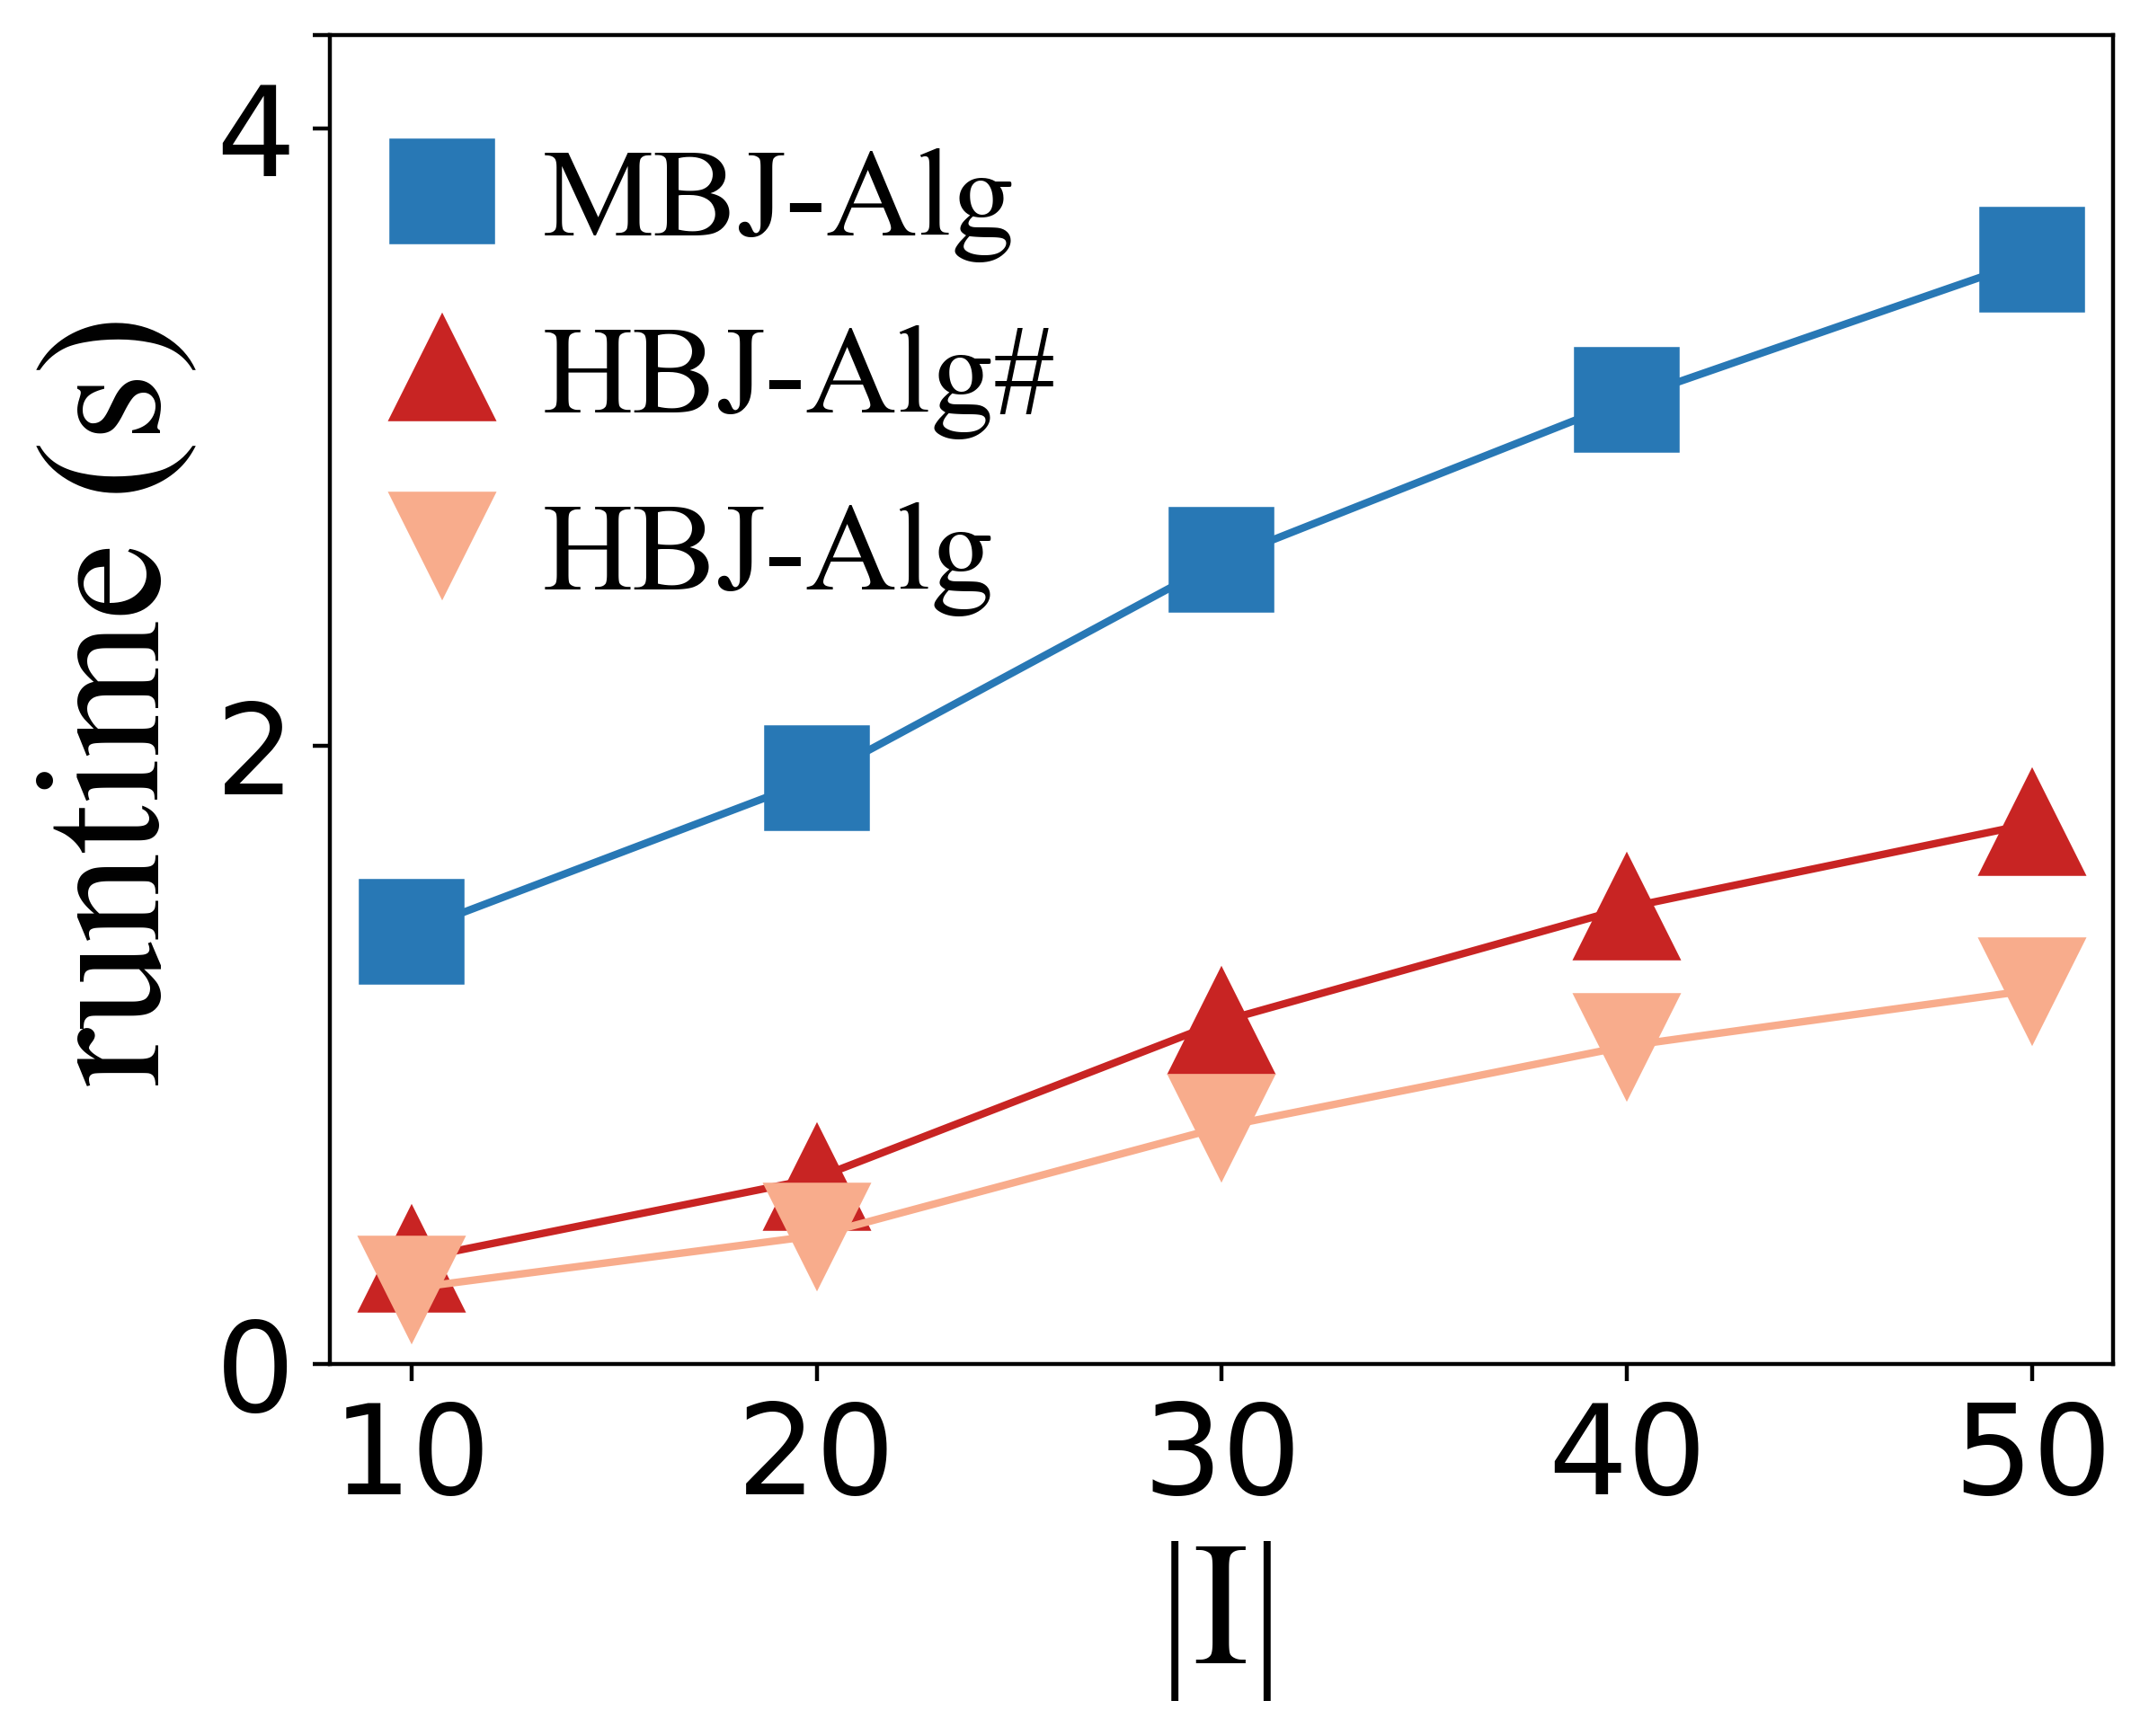
\includegraphics[width=0.4\textwidth]{fig/section6/geo-I-ftime.png}
    \label{geo-I-ftime}
}% 
\hfill
 \subfloat[]{
    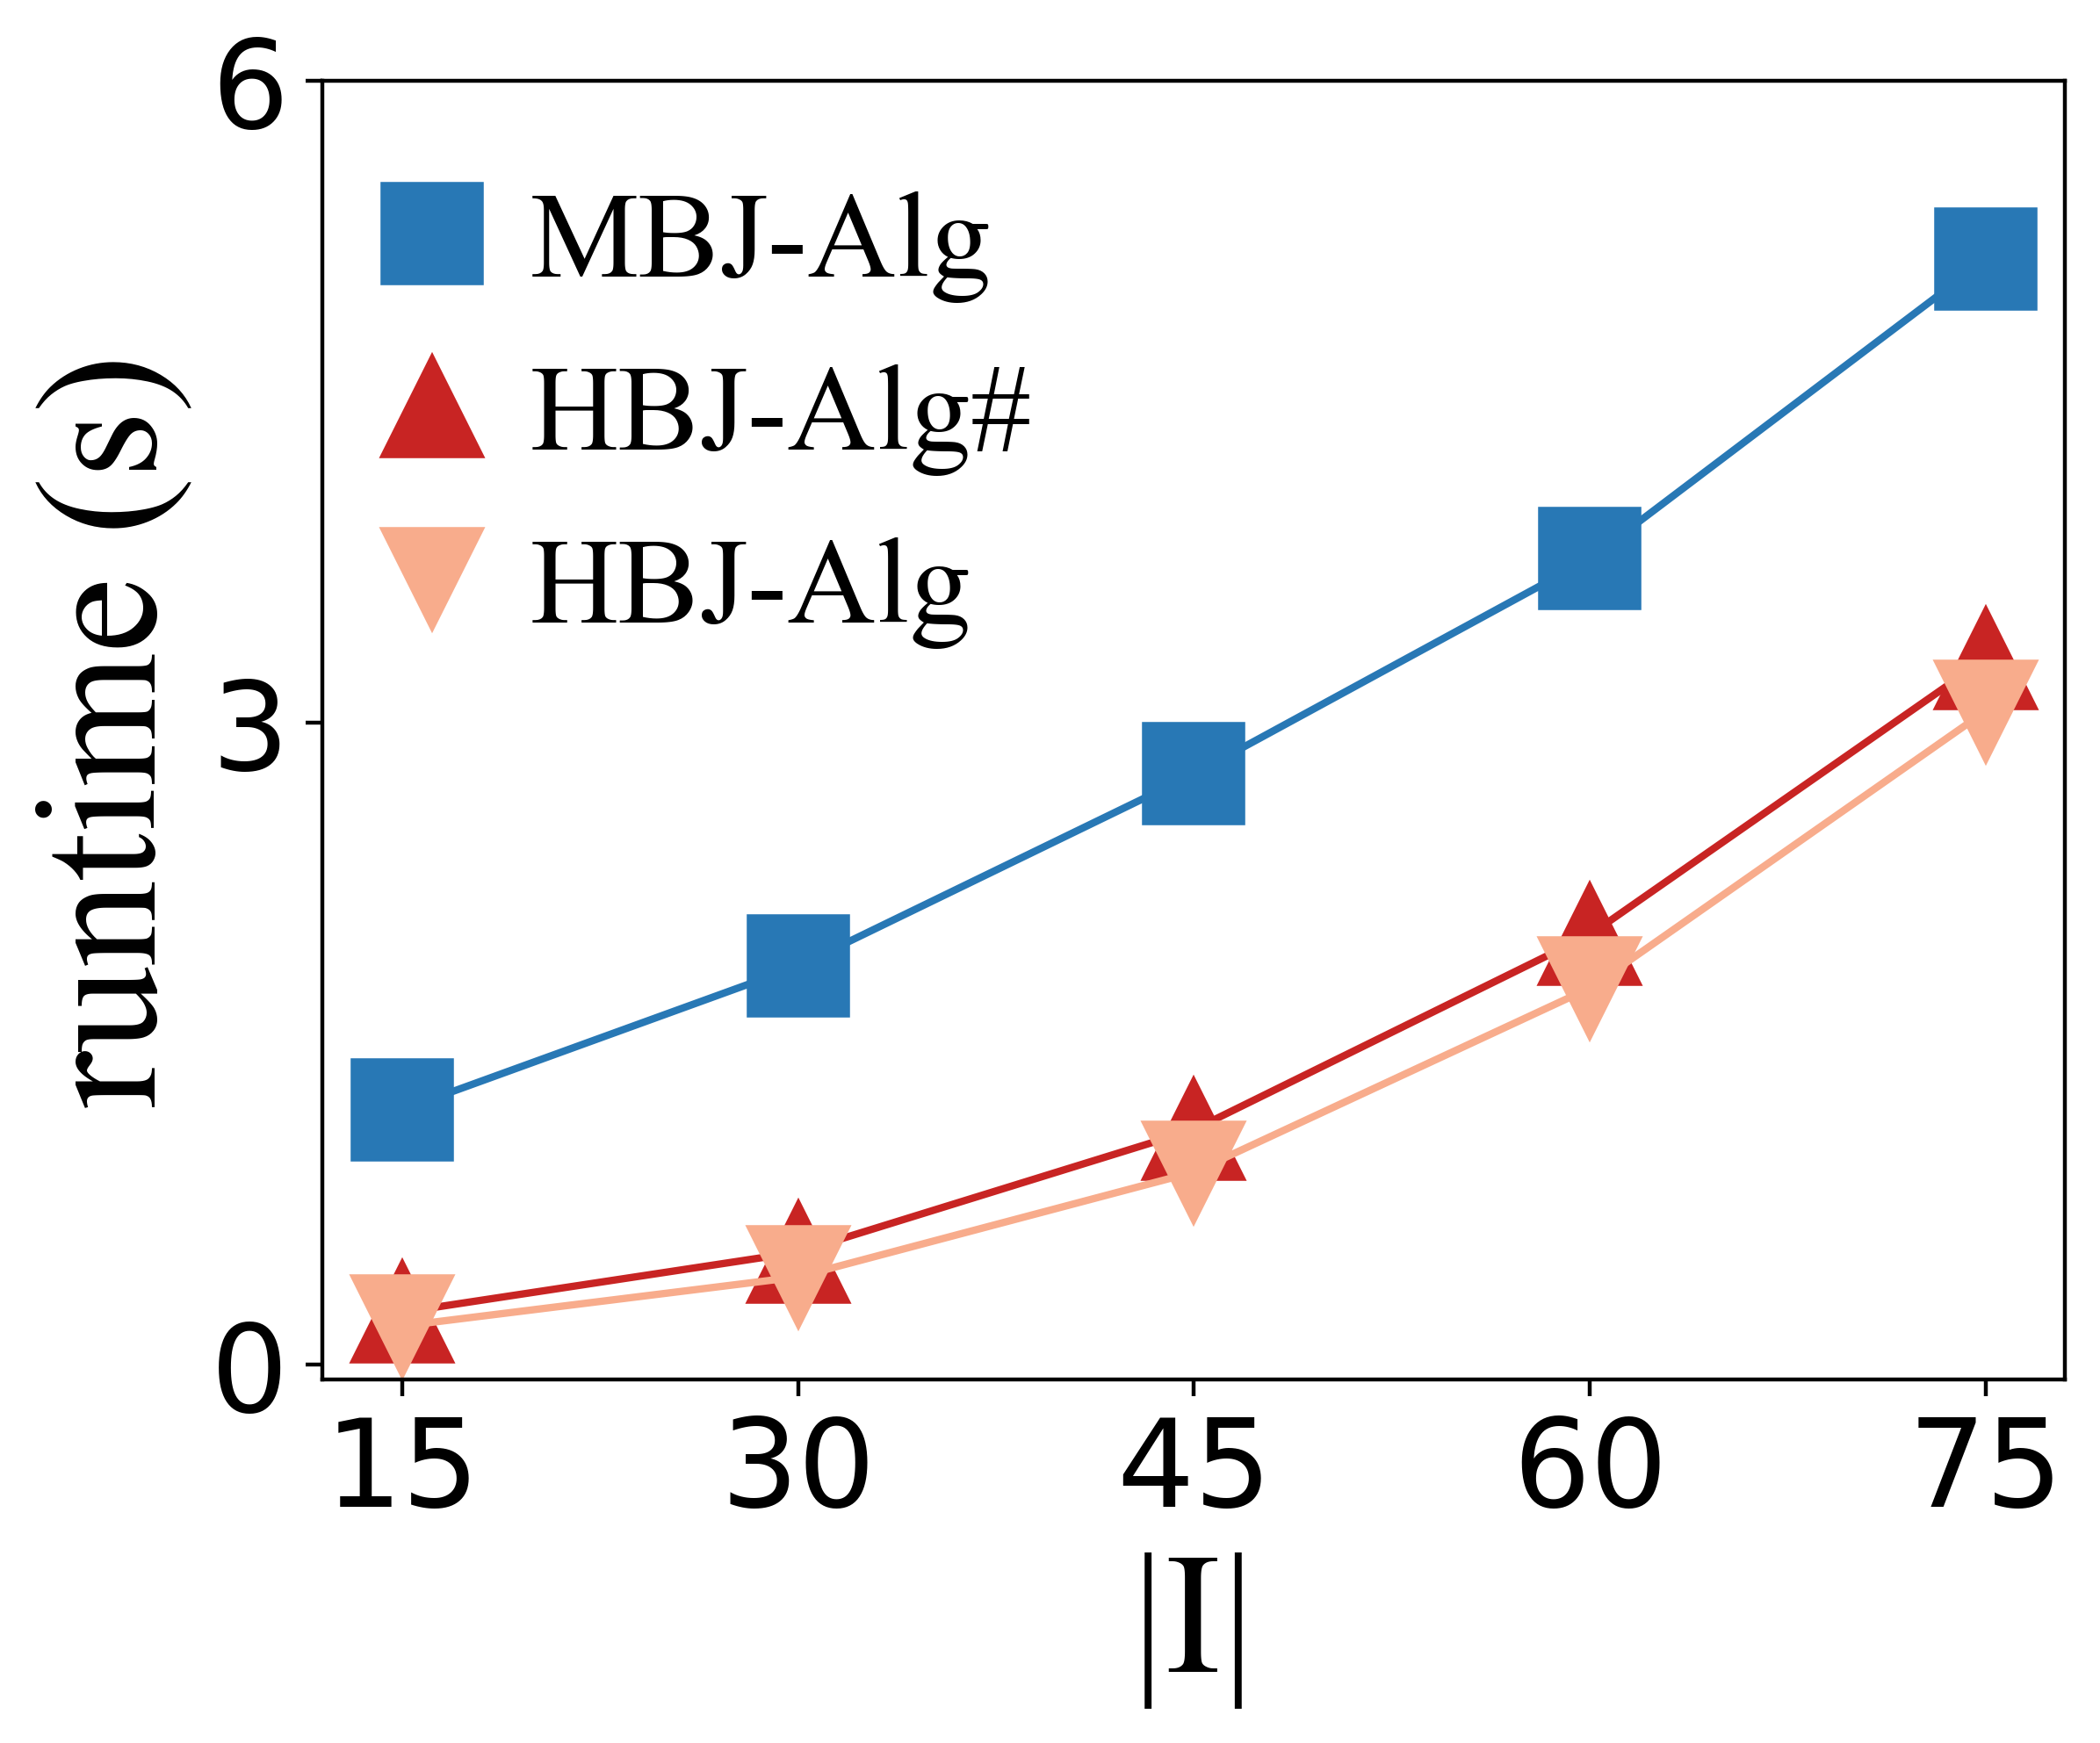
\includegraphics[width=0.4\textwidth]{fig/section6/pt-I-ftime.png}
    \label{pt-I-ftime}
}% 
\caption{$|I|$ 对运行时间的影响 \subref{geo-I-ftime}:Geolife数据集下的实验; \subref{pt-I-ftime}:Porto数据集下的实验}
\label{img:vary_I_ftime}
\end{figure}

\subsubsection{$\epsilon$ 的影响}

较小的 $\epsilon$ 值意味着需要探测更多的时间点运动范围，使得放松后的相似度更加接近真实的交集相似度，从而带来更高的计算开销，并导致运行时间的增加。图~\ref{img:vary_ep_ftime} 展示了在变化放松参数 $\epsilon$ 时的效率表现。在实验中，我们将时间点运动范围的数量从 2 变化到 10。随着 $\epsilon$ 的变化，可以观察到运行时间呈现出轻微的上升趋势。同时也可以看到，在所有参数设置下，HBJ-Alg 始终表现出最优的性能。

\begin{figure}[tb]
    \centering
    \subfloat[]{
    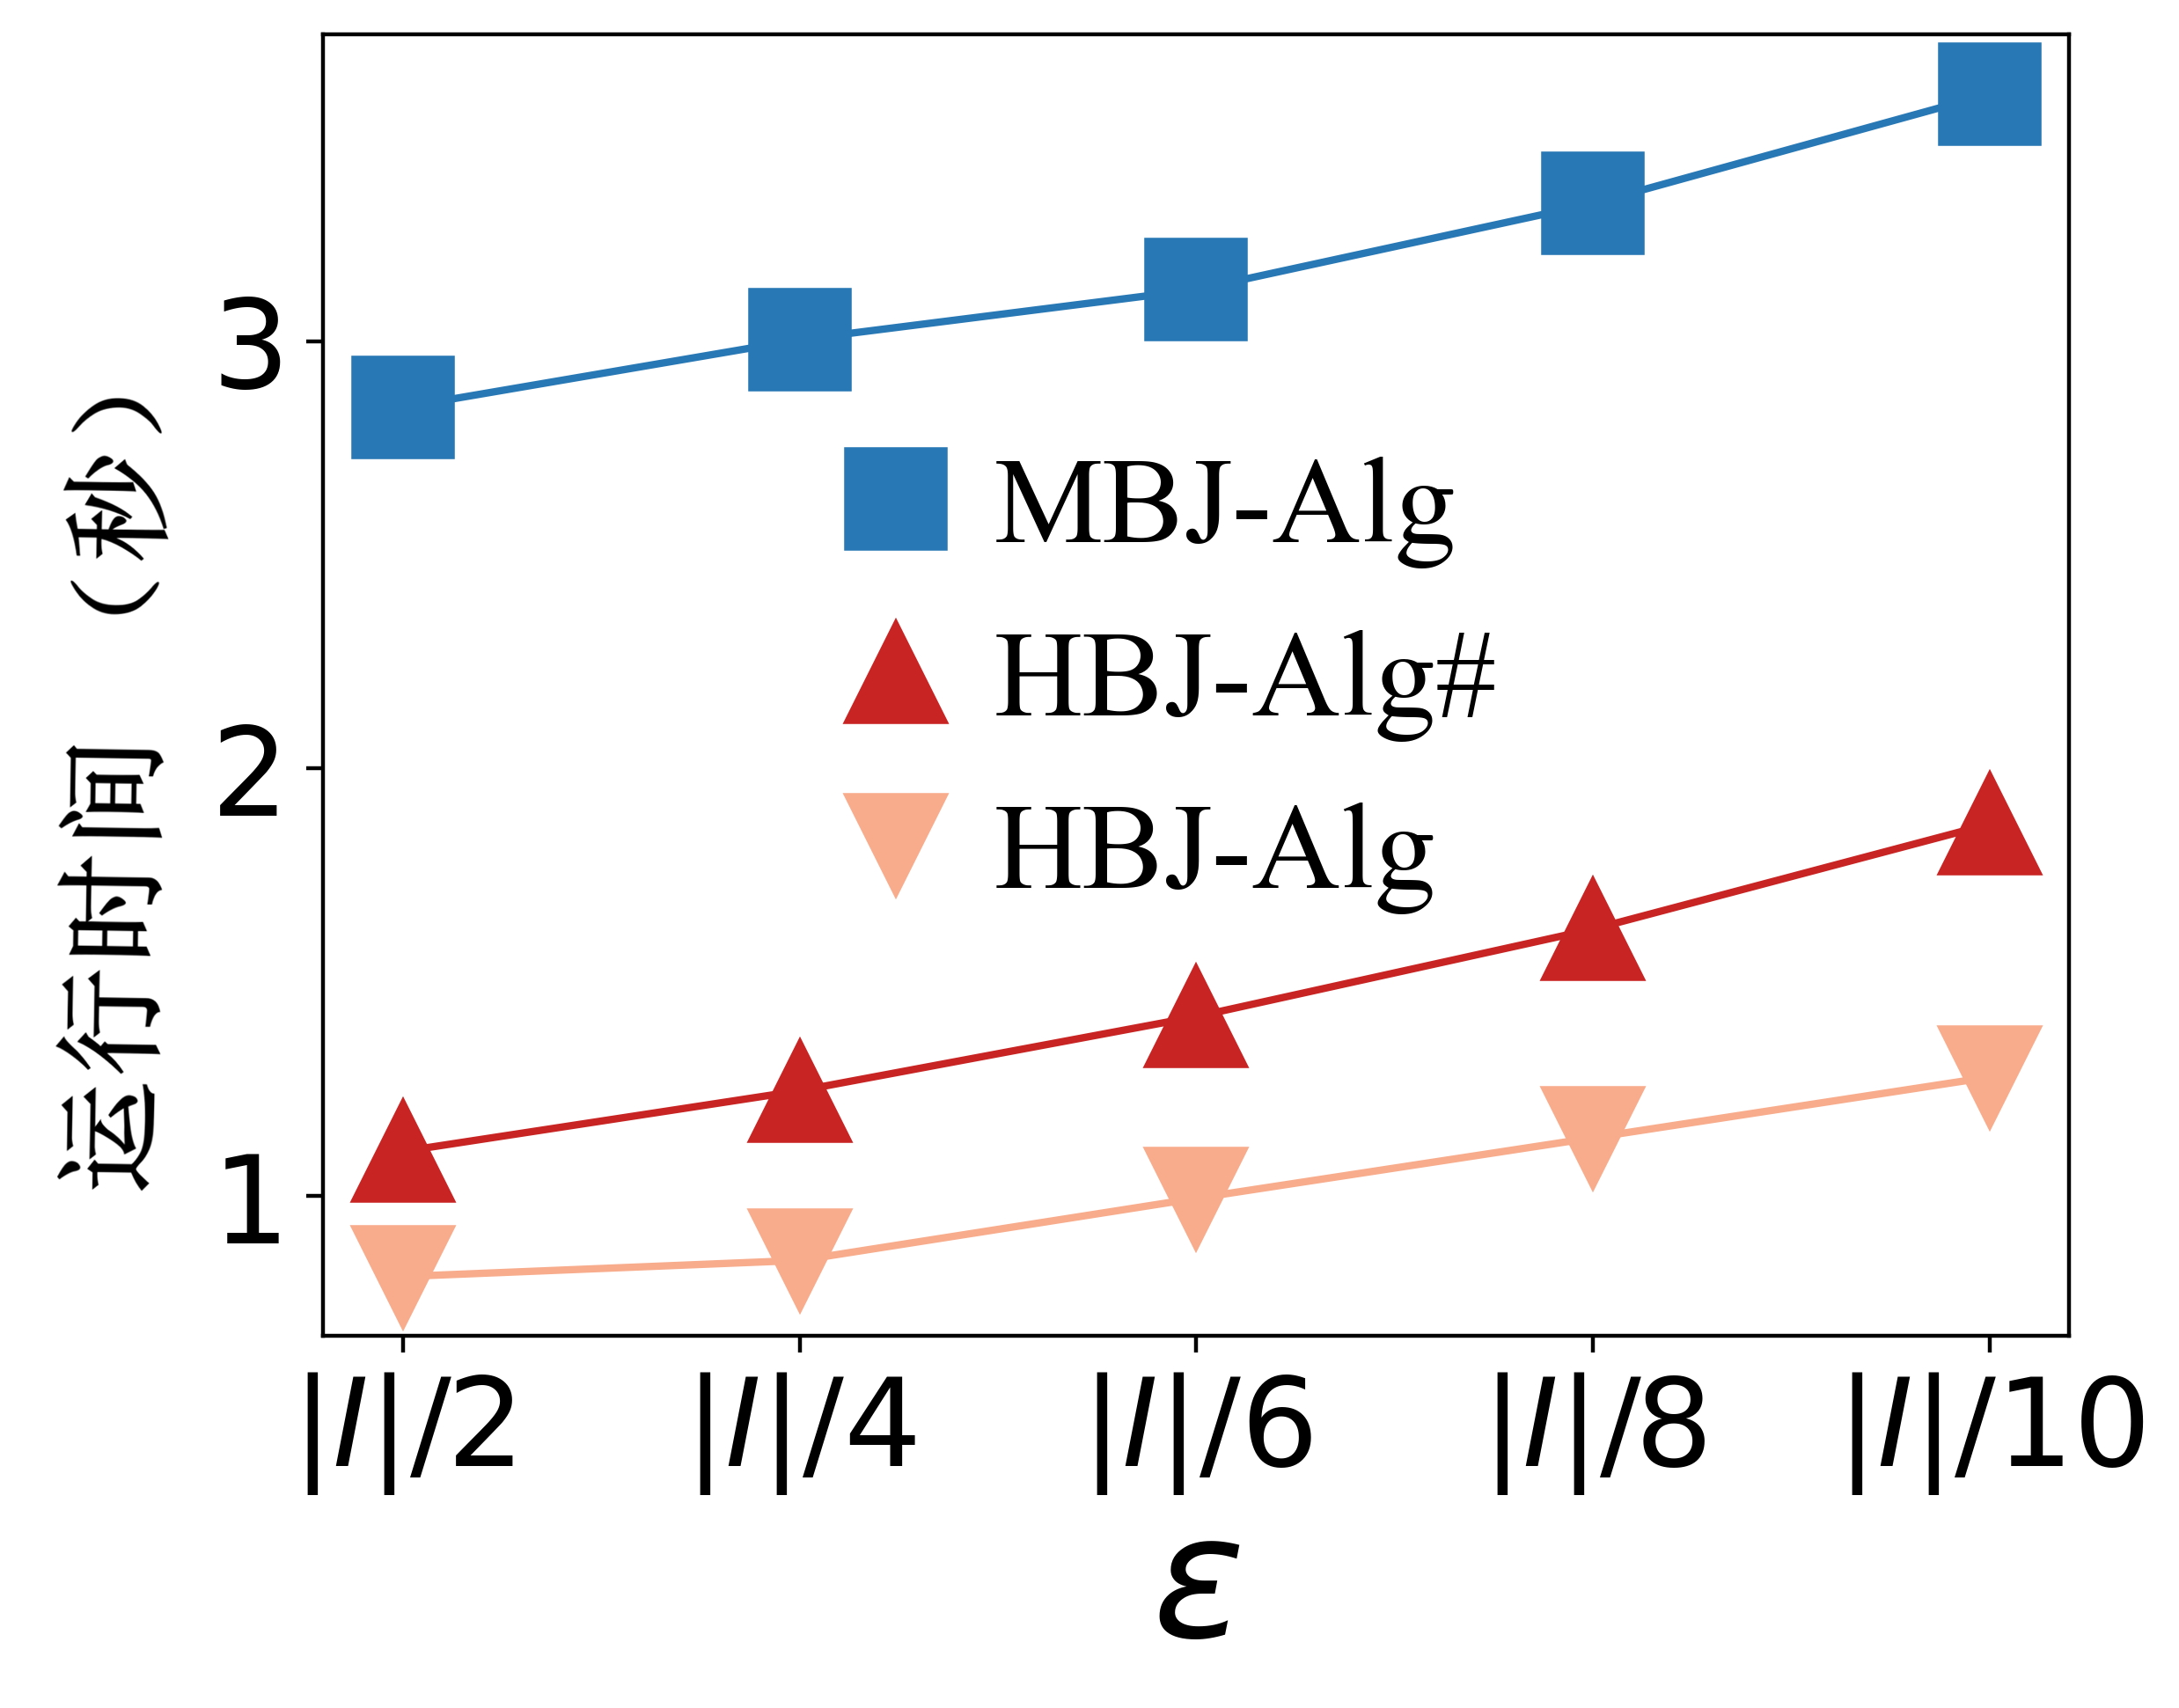
\includegraphics[width=0.4\textwidth]{fig/section6/geo-ep-ftime.png}
    \label{geo-ep-ftime}
}% 
\hfill
 \subfloat[]{
    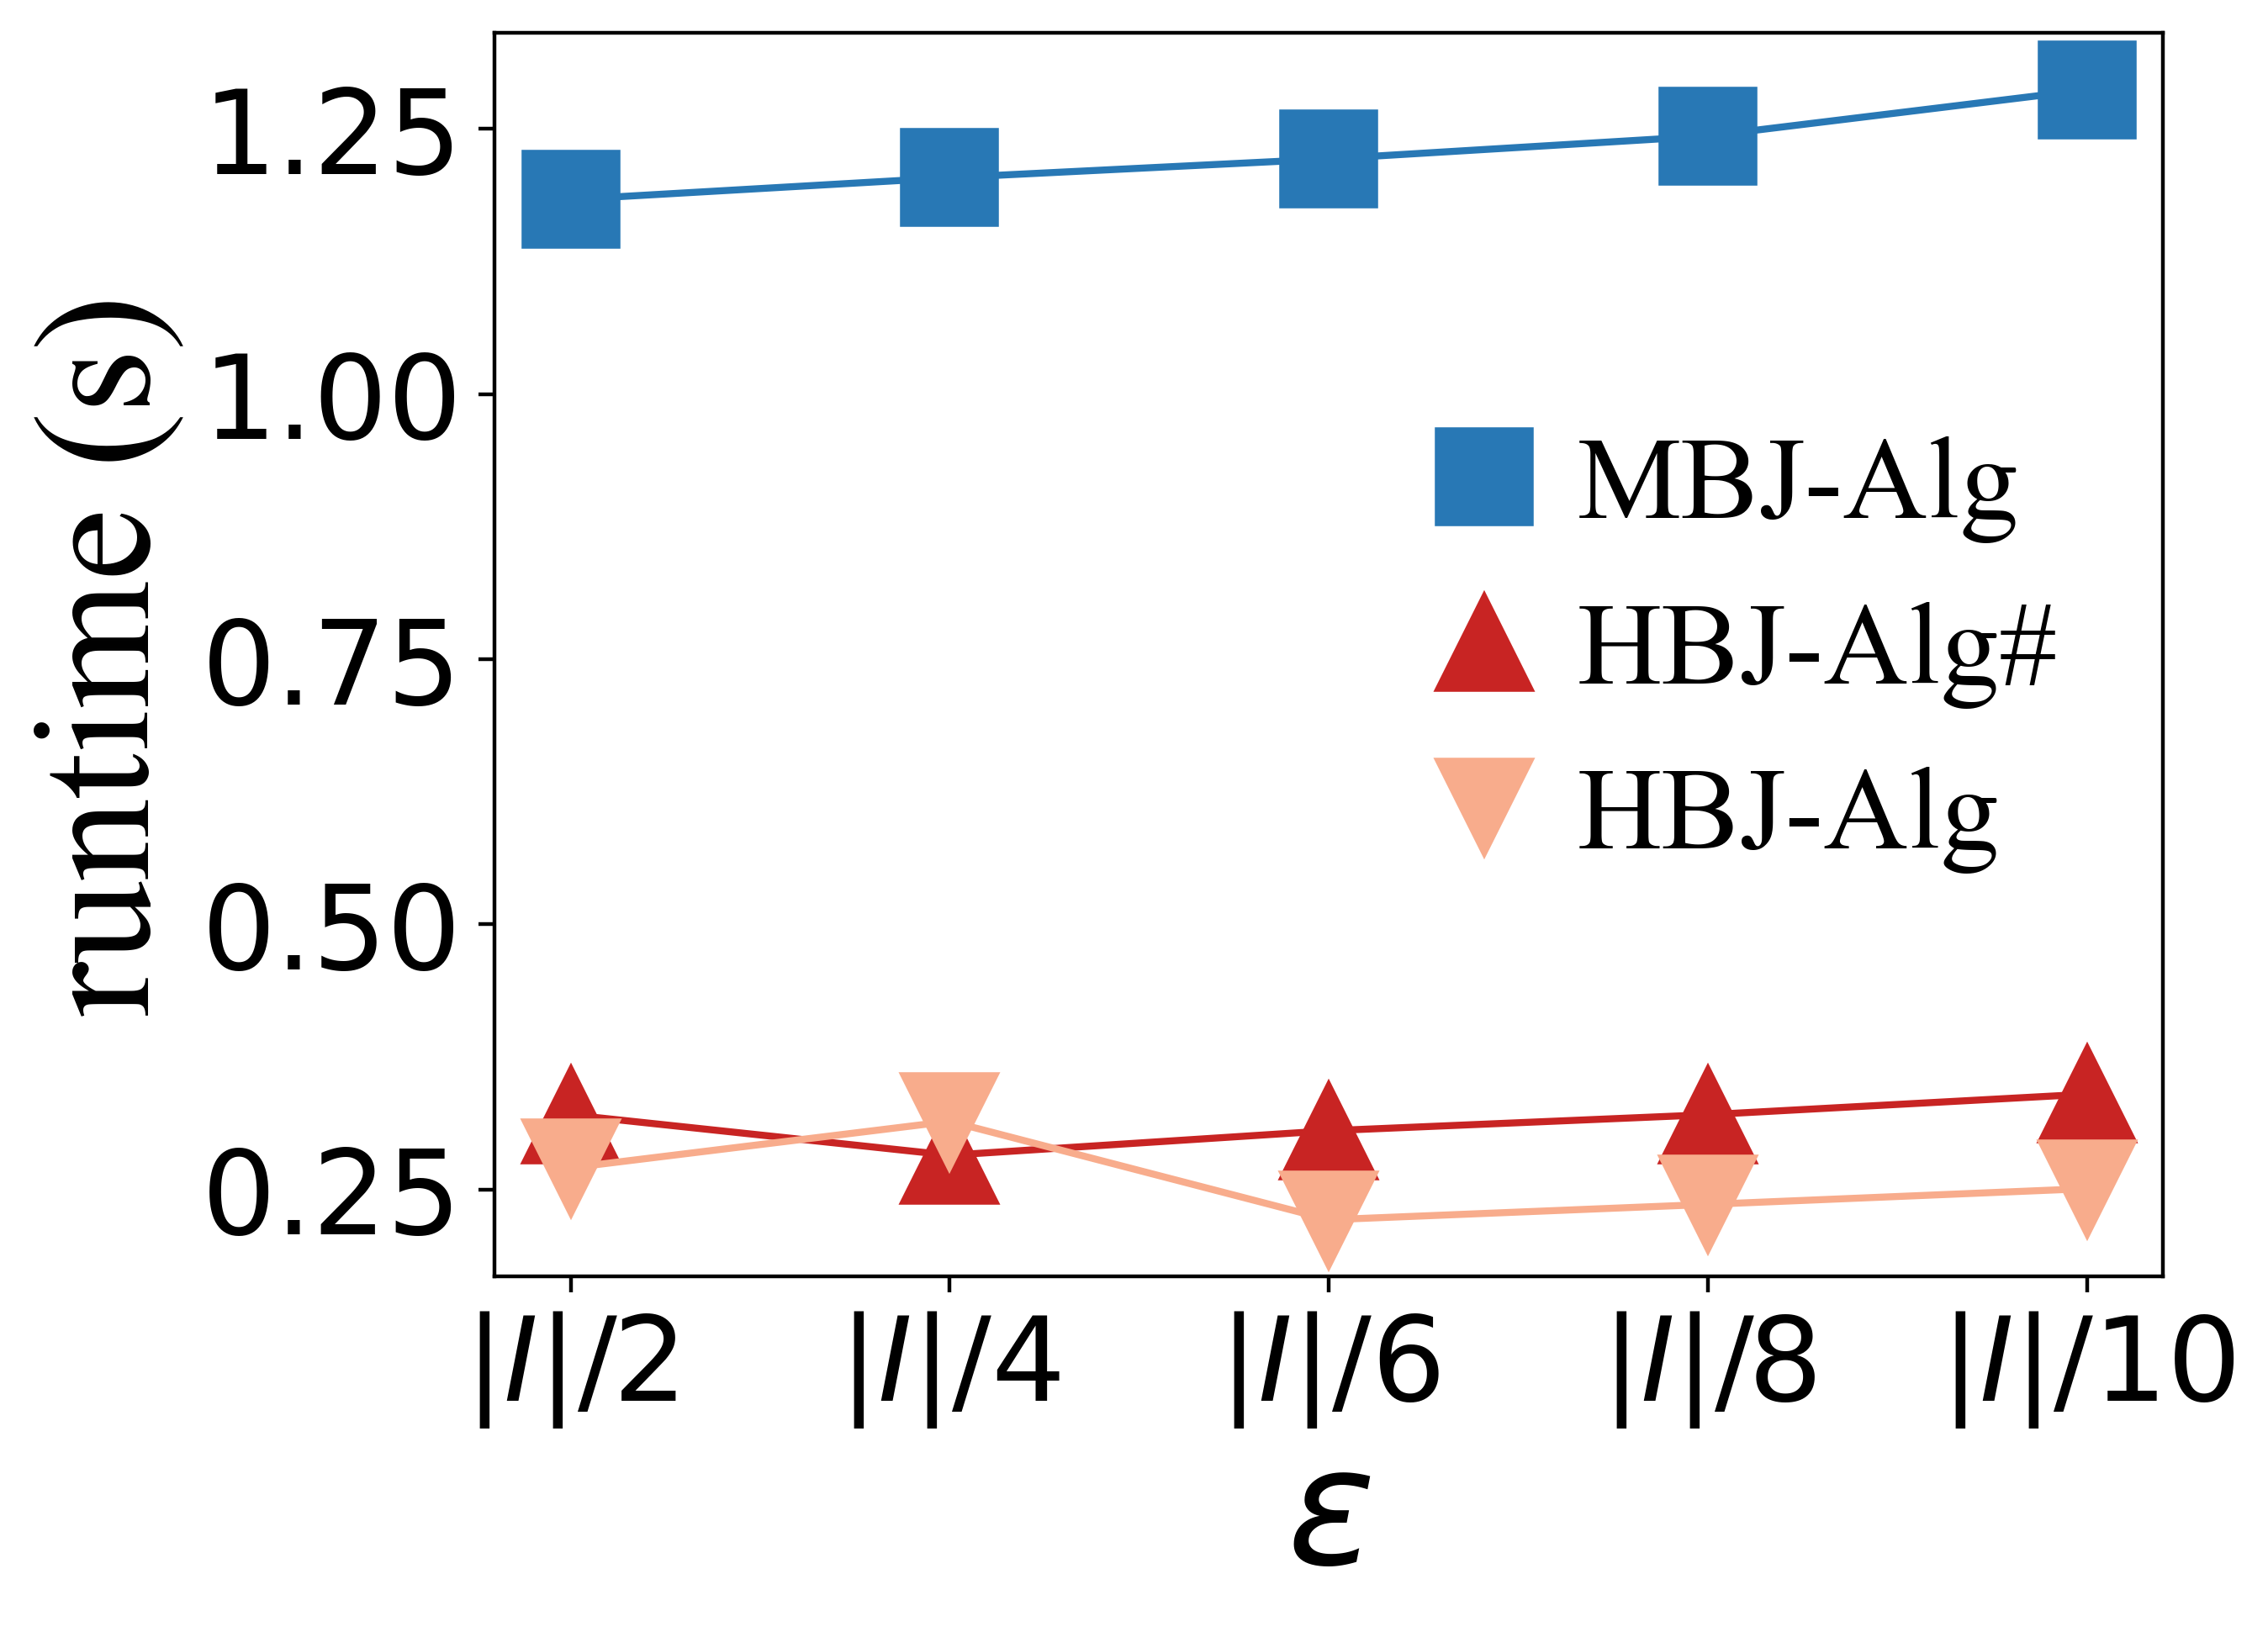
\includegraphics[width=0.4\textwidth]{fig/section6/pt-ep-ftime.png}
    \label{pt-ep-ftime}
}% 
\caption{参数 $\epsilon$ 的影响 \subref{geo-ep-ftime}:Geolife数据集下的实验; \subref{pt-ep-ftime}:Porto数据集下的实验}
\label{img:vary_ep_ftime}
\end{figure}




\section{基于 M*-树的连接算法}
\label{sec:baseLine}

\begin{algorithm}[!h]
    \caption{基于基本过滤与精炼的算法}
    \label{alg:bf-alg}
    
    \Input{
    两个移动对象集合，$\mathcal{A}$ 和 $\mathcal{B}$；\newline
    交集相似度阈值，$\theta$。
    }
    \Output{
    交集对，$\mathcal{R}$。
    }
    
    \textbf{初始化:} $\mathcal{L} \leftarrow \emptyset$；
    
    \For(\tcc*[f]{遍历集合 $\mathcal{A}$}){$o \in \mathcal{A}$}{
        \For(\tcc*[f]{遍历集合 $\mathcal{B}$}){$o' \in \mathcal{B}$}{
            \If{$dist(MR(o), MR(o')) \leq MR(o).a + MR(o').a$}{
                $\mathcal{L}.add((o, o'))$；
            }
        }
    }
    
    \For(\tcc*[f]{精炼步骤}){$(o, o') \in \mathcal{L}$}{
        \If{$IS(o, o', I, \epsilon) \geq \theta$}{
            $\mathcal{R} \leftarrow \{\mathcal{R}, (o, o')\}$；
        }
    }
    
    \textbf{return} $\mathcal{R}$；
    \end{algorithm}

首先，我们介绍一种基于 M*-树的连接算法（MBJ-Alg）用于计算 IS-Join，这作为基线方法。M*-树是 M-tree 的一种扩展~\cite{DBLP:conf/sebd/CiacciaPRZ97,DBLP:conf/vldb/CiacciaPZ97}。MBJ-Alg 是一个两阶段算法，结合了预检查策略，其中使用 M-tree 的变体来增强候选对象的过滤能力。

在阶段 1 中，M*-树使用近似圆来索引时间区间内的运动范围。这种圆形索引允许提前剪枝不合格对象，从而集中于更可能发生交集的候选对象。在阶段 2 中，对候选对象在时间点运动范围级别进行评估。下面将介绍 M*-树的结构及其在 IS-Join 查询中的应用。

\begin{figure}[htbp]
    \centering
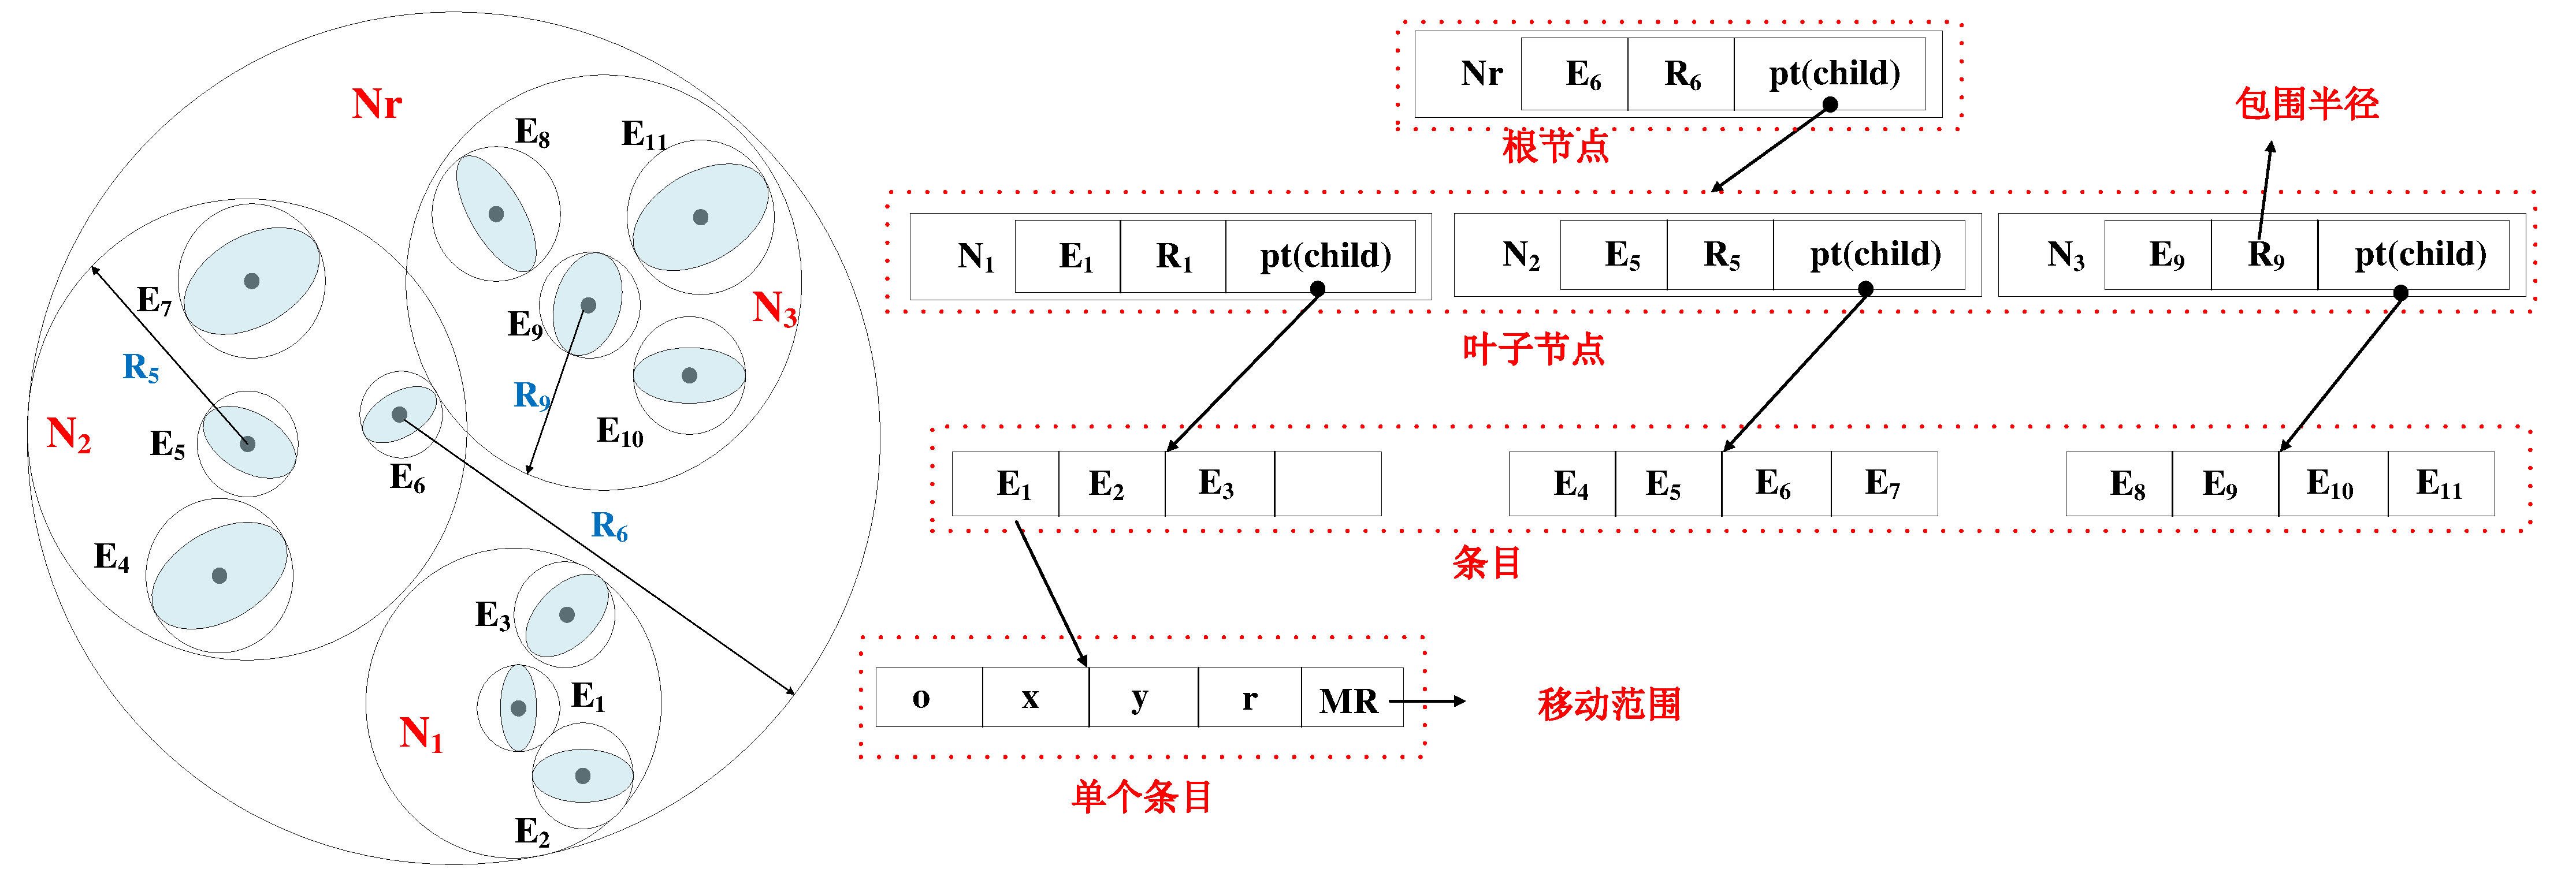
\includegraphics[width=1\textwidth]{fig/section6/mtree.pdf}
\caption{M*-树的结构}
\label{fig:m*-tree}
\end{figure}

\subsection{M*-树}

图~\ref{fig:m*-tree} 展示了 M*-树的结构，其指定容量为 $M=4$，表示每个叶节点的最大条目数。近似圆被视为单独的条目，并独立存储在叶节点中。我们使用近似圆表示时间区间的运动范围，并在 M*-树中对其进行索引。每个圆存储为条目 $E=\{o,x,y,r,MR(o,I)\}$，其中 $o$ 为对象标识，$(x, y)$ 表示圆心，$r$ 为半径，$MR(o,I)$ 包含时间区间的运动范围。M*-树中的每个节点 $N$ 选择叶节点中的一个条目 $E$ 作为其路由对象，格式为 $N=\{E,R,pt(child)\}$。这里，$E$ 是路由对象，$R$ 是能够覆盖 $N$ 中所有条目（即圆）的半径，$pt(child)$ 是指向子节点的指针。需要注意的是，M*-树在条目插入策略、节点分裂策略和路由对象选择策略上遵循了已有研究~\cite{DBLP:conf/edbt/ZhangRSL21,DBLP:conf/vldb/CiacciaPZ97} 的做法，并将这些策略适配到 M*-树结构中。

值得注意的是，同一 M*-树内的时间区间运动范围在时间上是对齐的。我们为特定时间区间索引所有运动范围，当时间区间改变时，需要重建 M*-树索引。

\subsection{交集检查}

我们从查询条目 $E_q=(q, x_q, y_q, r_q, MR(q,I))$ 和 M*-树的根节点开始。目标是检索所有可能与 $E_q$ 相交的条目 $E=\{o, x, y, r, MR(o,I)\}$。为了确定潜在交集，我们计算查询对象 $q$ 与每个条目 $E$ 之间的距离 $d(q, E)=\sqrt{(x_q-x)^2+(y_q-y)^2}$。如果 $d(q, E) \leq r + r_q$，则时间区间运动范围 $MR(q,I)$ 和 $MR(o,I)$ 可能相交。其中，$r$ 和 $r_q$ 分别表示条目 $E$ 和 $E_q$ 的半径。对于每个查询对象 $q$，我们索引所有满足 $d(q,E)\leq r+r_q$ 的条目，并将对应的 $(q,o)$ 加入候选集合，其中 $o$ 是与条目 $E$ 关联的对象标识。

\subsection{算法细节}
\begin{algorithm}[!h]
    \caption{$MBJ(\mathcal{A},\mathcal{B},N_r, I,\epsilon,\theta)$}
    \label{alg:MBJ-Join}
    
    \Input{
    两组移动对象，$\mathcal{A}$ 和 $\mathcal{B}$；\newline
    M*-树的根节点 $N_r$；\newline
    时间间隔 $I$；\newline
    分区参数 $\epsilon$；\newline
    交集相似度阈值 $\theta$。
    }
    \Output{
    $\mathcal{R} = \{(o,o') \mid IS(o,o',I,\epsilon) \geq \theta, (o,o') \in \mathcal{A} \times \mathcal{B}\}$。
    }
    
    \textbf{初始化:} $\mathcal{R} \leftarrow \emptyset$；
    
    \For(\tcc*[f]{遍历集合 $\mathcal{A}$}){$o \in \mathcal{A}$}{
        $\mathcal{L} \leftarrow \{N_r\}$；
    
        \While(\tcc*[f]{M*-树遍历}){$\mathcal{L} \neq \emptyset$}{
            $N \leftarrow \mathcal{L}.pop()$；
    
            \If(\tcc*[f]{非叶子节点}){$N$ 是非叶子节点}{
                \For(\tcc*[f]{遍历子节点}){$N_c \in N.pt(child)$}{
                    \If{$d(o, N_c) \leq N_c.R + o.r$}{
                        $\mathcal{L}.push(N_c)$；
                    }
                }
            }
            \Else(\tcc*[f]{叶子节点处理}){
                \If{$d(o, N) > N.R + o.r$}{
                    $prune(o, N.o)$;\tcp*[f]{预检查策略}
                }
    
                \If{$IS(o, N.o, I, \epsilon) \geq \theta$}{
                    $\mathcal{R} \leftarrow \{\mathcal{R}, (o, N.o)\}$;\tcp*[f]{精炼步骤}
                }
            }
        }
    }
    \textbf{return} $\mathcal{R}$；
    \end{algorithm}
    
    算法~\ref{alg:MBJ-Join} 给出了基于 M*-树的两阶段剪枝匹配算法（MBJ-Alg）的伪代码。算法的输入包括两个移动对象集合、M*-树的根节点、带分区参数 $\epsilon$ 的时间区间，以及相似度阈值 $\theta$。我们使用列表 $\mathcal{R}$ 存储所有满足条件的对象对，初始时 $\mathcal{R}$ 为空（第 1 行）。  

    该算法由两个阶段组成：(1) 基于 M*-树的预检查（第 3--12 行），以及 (2) 精炼过程（第 13--14 行）。在预检查阶段，我们根据 M*-树获取候选对象集合。我们使用列表 $\mathcal{L}$ 存储可能与移动对象相交的节点，初始时 $\mathcal{L}$ 仅包含根节点（第 3 行）。  
    
    当 $\mathcal{L}$ 非空时，我们从中取出与对象 $o$ 的距离 $d(o,N)$ 最小的 M*-树节点 $N$（第 5 行）。如果 $N$ 不是叶节点，则考虑其子节点。对于 $N$ 的每个子节点 $N_c$，我们检查 $o$ 与 $N_c$ 之间的距离。如果该距离不大于 $o$ 与 $N_c$ 半径之和，则将 $N_c$ 压入优先队列（第 7--9 行）。  
    
    如果 $N$ 是叶节点，且 $d(o,N) > N.R + o.r$，则可以安全地剪枝 $(o, N.o)$（第 11--12 行）。当交集相似度不小于阈值 $\theta$ 时，我们通过将 $(o, N.o)$ 添加到结果集来更新 $\mathcal{R}$（第 14 行）。  
    
    最后，返回 $\mathcal{R}$ 作为得到的交集对象对（第 15 行）。

    \subsubsection{时间复杂度分析}

    一般来说，构建 M*-树需要 $O(|\mathcal{B}|\times n)$ 的时间，其中 $\mathcal{B}$ 是被 M*-树索引的对象集合，$n$ 是节点分裂操作的次数。具体来说，当由于对象插入导致节点已满时，需要将其分裂为多个节点，这一操作的时间复杂度为 $O(|\mathcal{B}|)$。值得注意的是，实际构建时间可能会因数据分布等因素而有所不同。  
    
    设 $\mathcal{A}$ 为查询对象集合。为了找到所有候选对象，过滤过程的时间复杂度为 $O(|\mathcal{A}|\times\log|\mathcal{B}|)$。若时间点运动范围内的 POI 平均数量为 $p$，则每次计算 $IS(o,o',I,\epsilon)$ 的时间复杂度为 $O(|I|/\epsilon \times p)$。  
    
    设 $\mathcal{C}$ 为候选对象集合。对候选对象进行精炼的时间复杂度为 $O(|\mathcal{C}|\times |I|/\epsilon \times p)$。  
    
    因此，MBJ-Alg 每轮执行的总时间复杂度为
    \[
    O\big(|\mathcal{B}|\times n + |\mathcal{A}|\times\log|\mathcal{B}| + |\mathcal{C}|\times |I|/\epsilon \times p\big)。
    \]

    \section{Top-$k$ 交集相似度连接}

我们的方法可以很容易扩展以支持 top-$k$ 交集相似度连接（$k$-IS-Join），定义如下。与普通 IS-Join 不同，$k$-IS-Join 不需要阈值参数，而是返回两个集合中前 $k$ 个最相似的轨迹对。

\begin{definition}[$k$-IS-Join]\label{defi:k-IS-Join}
Top-\underline{k} \underline{交}集 \underline{相}似度连接（$k$-IS-Join）从两个对象集合中找到 $k$ 个最相似的对象对集合 $\mathcal{R}$，即 $|\mathcal{R}|=k$，且满足 $\forall (o_i,o_j)\in \mathcal{R} (\forall (o_i^{'},o_j^{'})\in (\mathcal{A}\times \mathcal{B})\setminus \mathcal{R}$，有
$(IS(o_i,o_j,I,\epsilon)>IS(o_i^{'},o_j^{'},I,\epsilon)))$。
\end{definition}

算法~\ref{alg:kMBJ-Join} 和算法~\ref{alg:kHBJ-Join} 分别给出了基于 M*-树和 HBall-树的 $k$-IS-Join 解法。


\begin{algorithm}[!h]
    \caption{$kMBJ(\mathcal{A},\mathcal{B},N_r,I,\epsilon,k)$}
    \label{alg:kMBJ-Join}
    
    \Input{
    两个移动对象集合，$\mathcal{A}$ 和 $\mathcal{B}$；\newline
    M*-树的根节点 $N_r$；\newline
    时间区间 $I$；\newline
    分区参数 $\epsilon$；\newline
    参数 $k$。
    }
    \Output{
    $\mathcal{R} =$ top-$k$ 对象对。
    }
    
    \textbf{初始化:} $\mathcal{R} \leftarrow$ 大小为 $k$ 的优先队列 PriorityQueue$\langle (o,o'), sim \rangle$；
    
    \For(\tcc*[f]{遍历集合 $\mathcal{A}$}){$o \in \mathcal{A}$}{
        $\mathcal{L} = N_r.query(MR(o,I))$；
    
        \For(\tcc*[f]{遍历候选对象}){$o' \in \mathcal{L}$}{
            $sim_k = \mathcal{R}.top().sim$；
    
            \If{$|\mathcal{R}| < k$}{
                $\mathcal{R}.push((o,o'), sim)$；
            }
            \ElseIf{$IS(o,o',I,\epsilon) \geq sim_k$}{
                $\mathcal{R}.push((o,o'), sim)$；
                $\mathcal{R}.poll()$；
            }
        }
    }
    
    \textbf{return} $\mathcal{R}$；
    \end{algorithm}



\begin{algorithm}[!h]
    \caption{$kHBJ(\mathcal{A},\mathcal{B},N_r,I,\epsilon,k)$}
    \label{alg:kHBJ-Join}
    
    \Input{
    两个移动对象集合，$\mathcal{A}$ 和 $\mathcal{B}$；\newline
    HBall-树的根节点 $N_r$；\newline
    时间区间 $I$；\newline
    分区参数 $\epsilon$；\newline
    参数 $k$。
    }
    \Output{
    $\mathcal{R} =$ top-$k$ 对象对。
    }
    
    \textbf{初始化:} $\mathcal{R} \leftarrow$ 大小为 $k$ 的优先队列 PriorityQueue$\langle (o,o'), sim \rangle$；
    
    \For(\tcc*[f]{遍历集合 $\mathcal{A}$}){$o \in \mathcal{A}$}{
        $\mathcal{L} = N_r.query(MR(o,I))$；
    
        \For(\tcc*[f]{遍历候选对象}){$o' \in \mathcal{L}$}{
            $sim_k = \mathcal{R}.top().sim$；
    
            \If{$|\mathcal{R}| < k$}{
                $\mathcal{R}.push((o,o'), sim)$；
            }
            \Else{
                \If{$IS(o,o',I,\epsilon)_{ub}^{'} < \theta$}{
                    \textbf{continue}；\tcp*[f]{时间点剪枝}
                }
                \If{$IS(o,o',I,\epsilon) \geq sim_k$}{
                    $\mathcal{R}.push((o,o'), sim)$；
                    $\mathcal{R}.poll()$；
                }
            }
        }
    }
    
    \textbf{return} $\mathcal{R}$；
    \end{algorithm}



\section{IS-Join 的附加实验}

\subsubsection{相似度阈值的影响}
对于 HBJ-Alg，增加相似度阈值 $\theta$ 可以提高剪枝效果。较大的 $\theta$ 减少搜索空间，从而降低 CPU 时间和访问的时间区间运动范围数量。图~\ref{img:vary_sim_ftime} 展示了在改变相似度阈值时的效率表现。与 MBJ-Alg 对比，HBJ-Alg 在所有设置下均优于 MBJ-Alg，运行时间最多可提升 3 倍。虽然 HBJ-Alg 在较高阈值下运行时间略有下降，但 MBJ-Alg 和 HBJ-Alg\# 的趋势不明显。

\begin{figure}[tb]
    \centering
    \subfloat[]{
        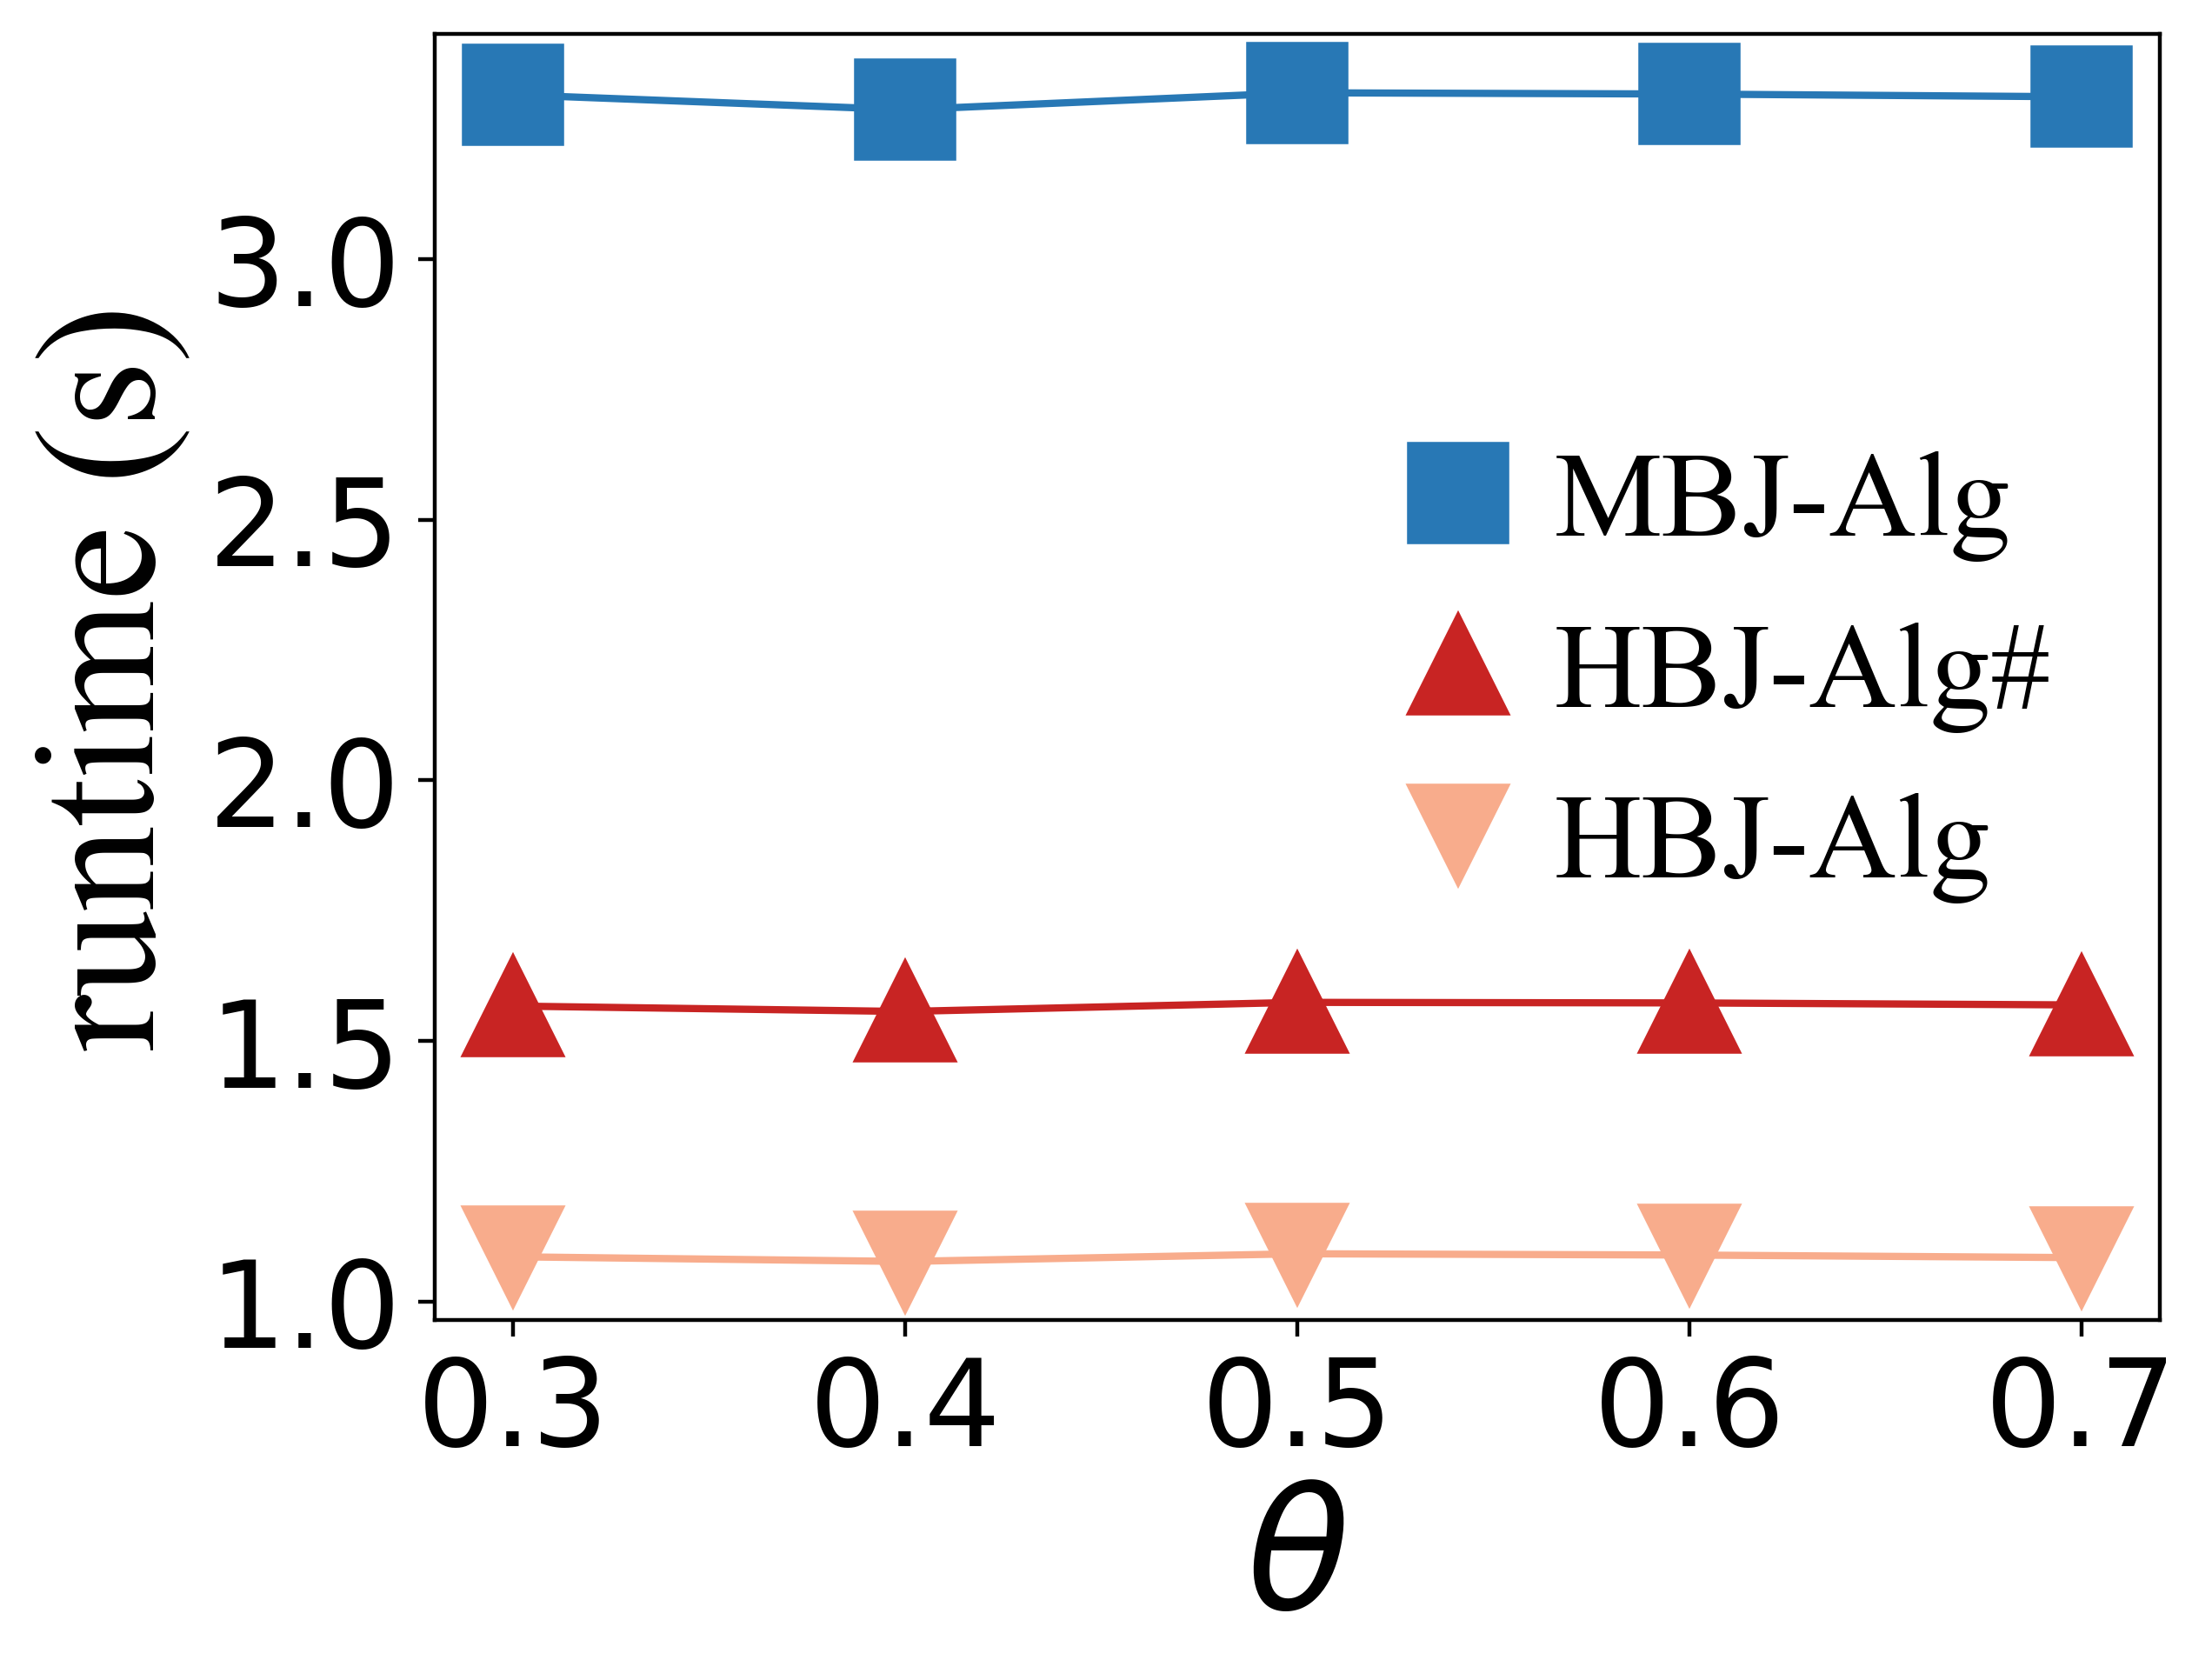
\includegraphics[width=0.4\textwidth]{fig/section6/geo-sim-ftime.png}
        \label{geo-sim-totaltime}
    }%
    \hfill
    \subfloat[]{
        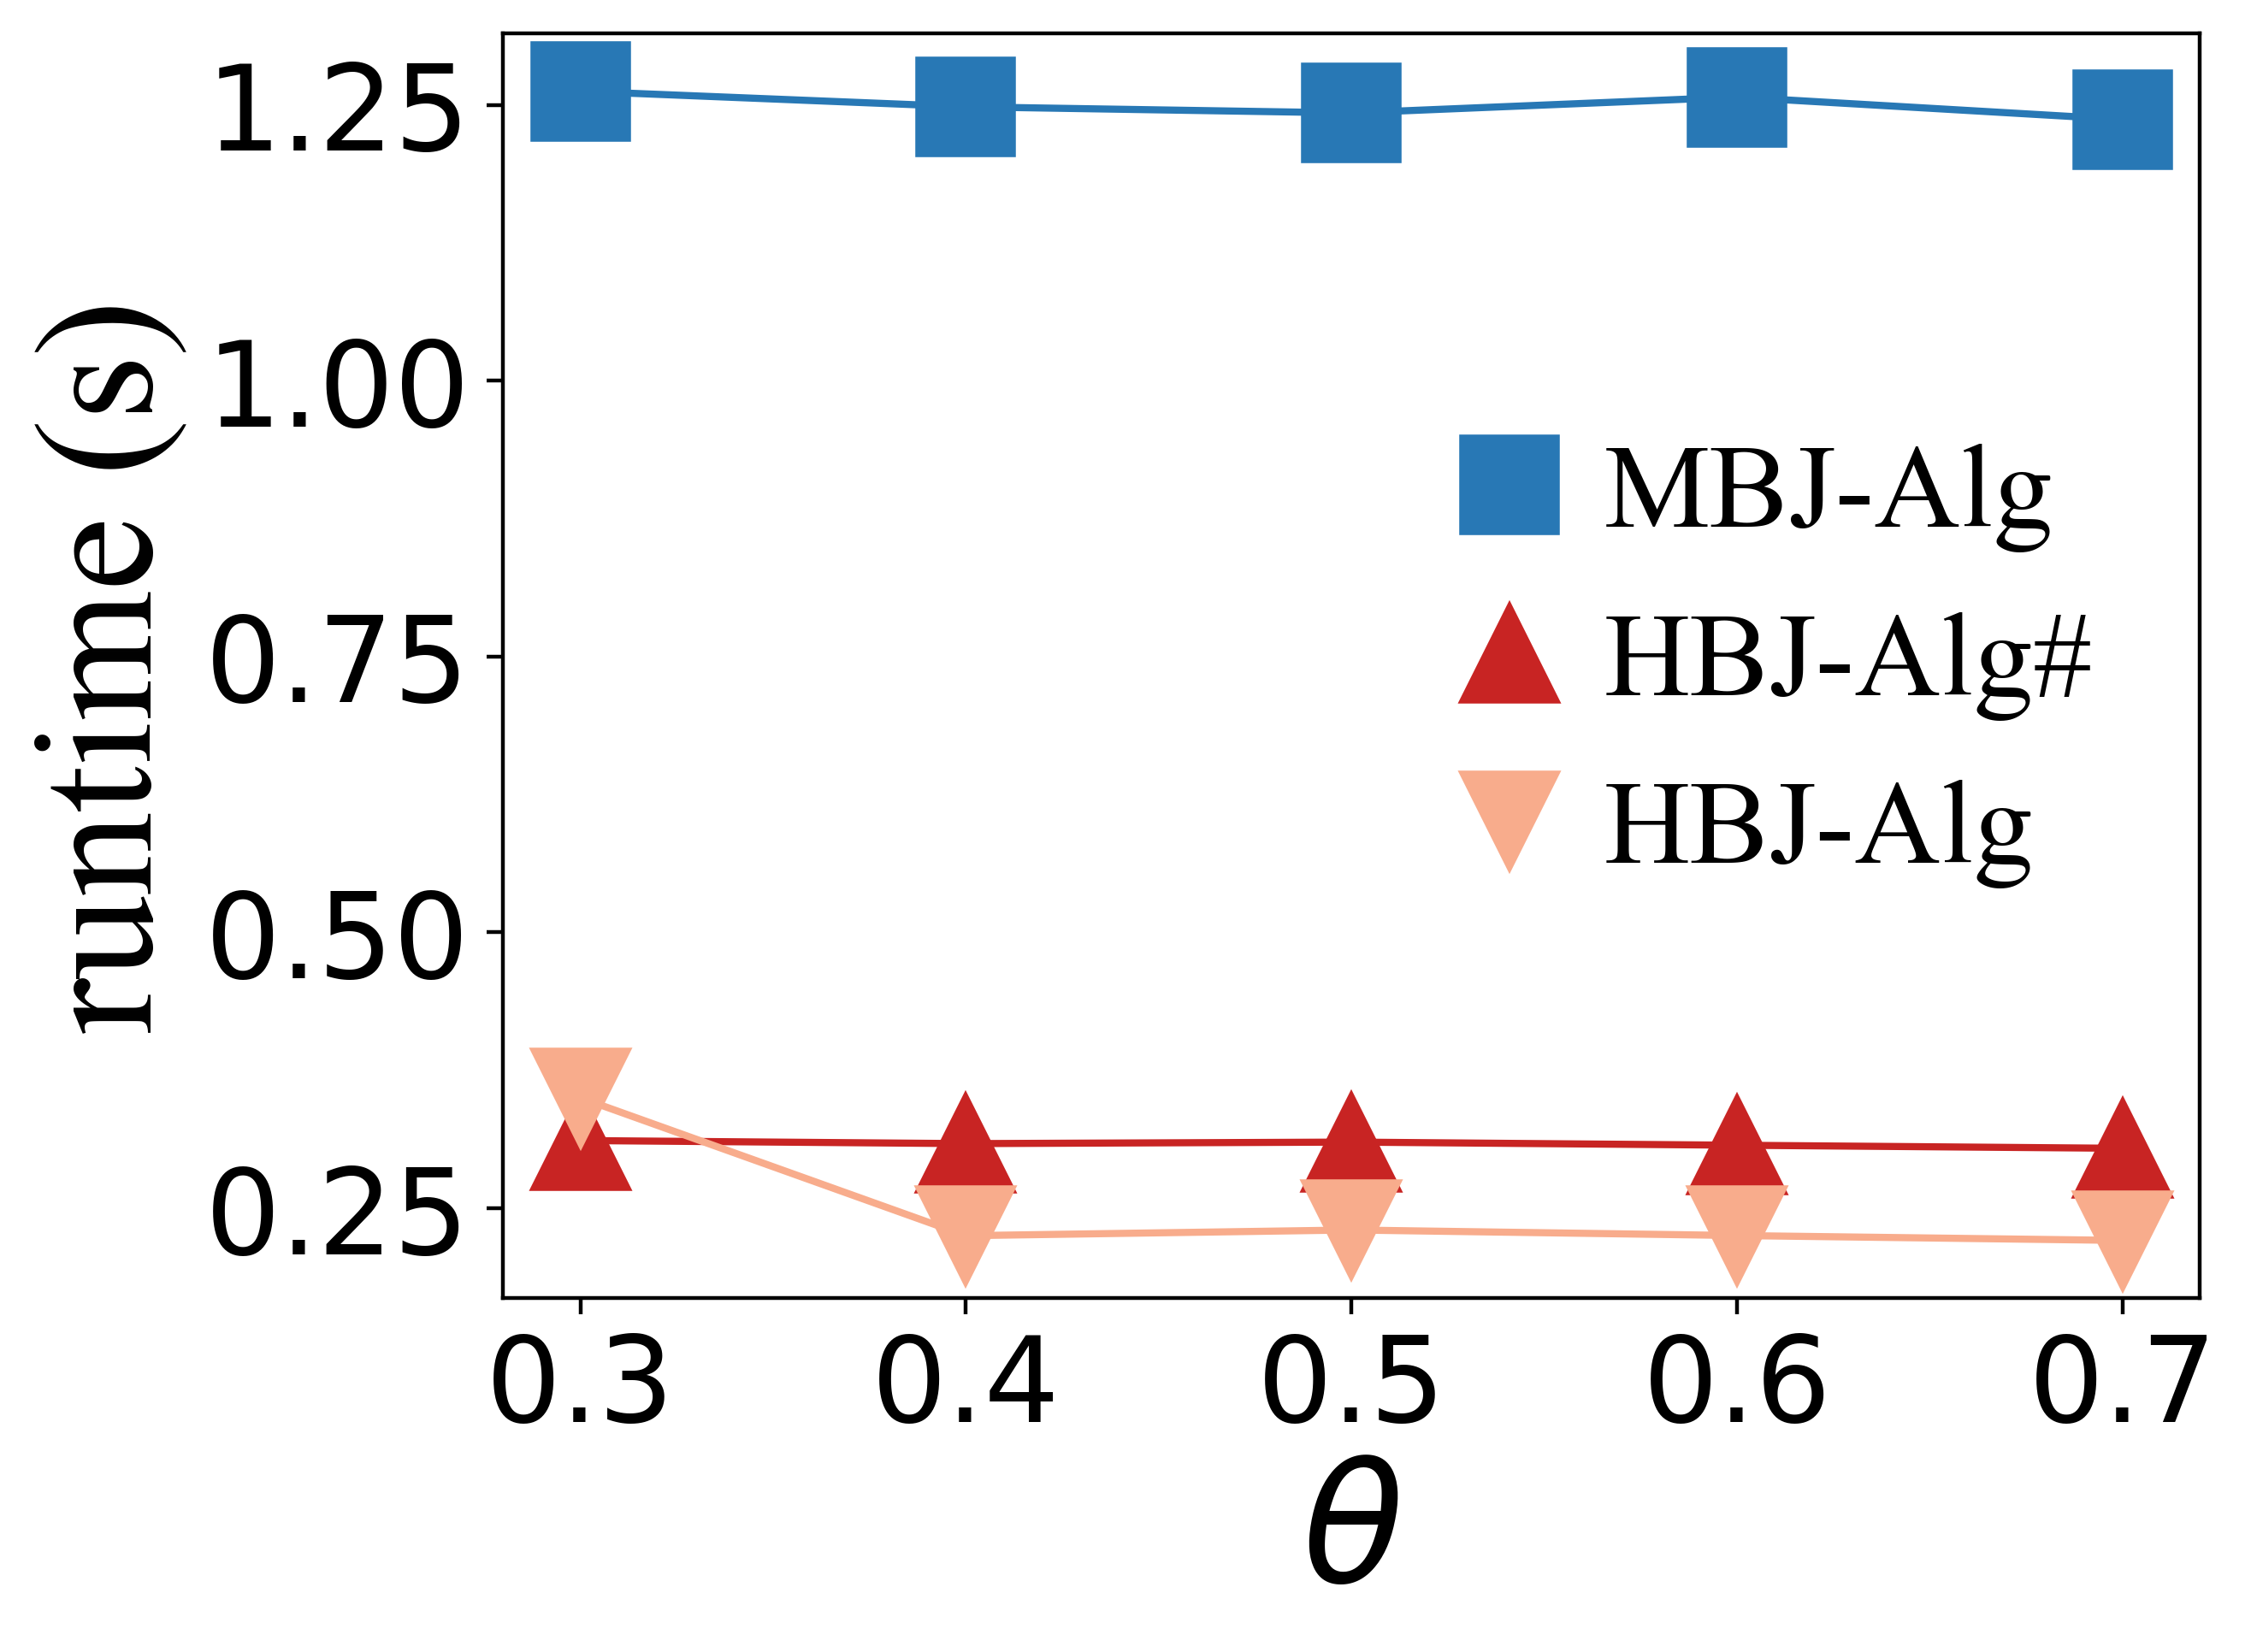
\includegraphics[width=0.4\textwidth]{fig/section6/pt-sim-ftime.png}
        \label{pt-sim-totaltime}
    }%
    \caption{相似度阈值的影响 \subref{geo-sim-totaltime}:Geolife数据集下的实验; \subref{pt-sim-totaltime}:Porto数据集下的实验}
    \label{img:vary_sim_ftime}
\end{figure}

\subsubsection{重新分区策略的评估}
我们比较 HBJ-Alg 和 HBJ-Alg$*$ 的性能，主要指标为节点访问总次数。图~\ref{img:vary_num_access} 显示了移动对象数量对重新分区策略性能的影响（默认设置）。随着移动对象数量增加，节点访问总数也增加。HBJ-Alg 与 HBJ-Alg$*$ 的性能差距随对象数量增长而扩大。HBJ-Alg 的重新分区策略可在不增加索引构建时间的情况下，将节点访问数减少约 10\%，甚至可能降低索引构建时间（见图~\ref{img:vary_num_ctime}）。因此，重新分区策略有助于提升整体效率，处理大规模数据集时更有效。

\begin{figure}[tb]
    \centering
    \subfloat[]{
        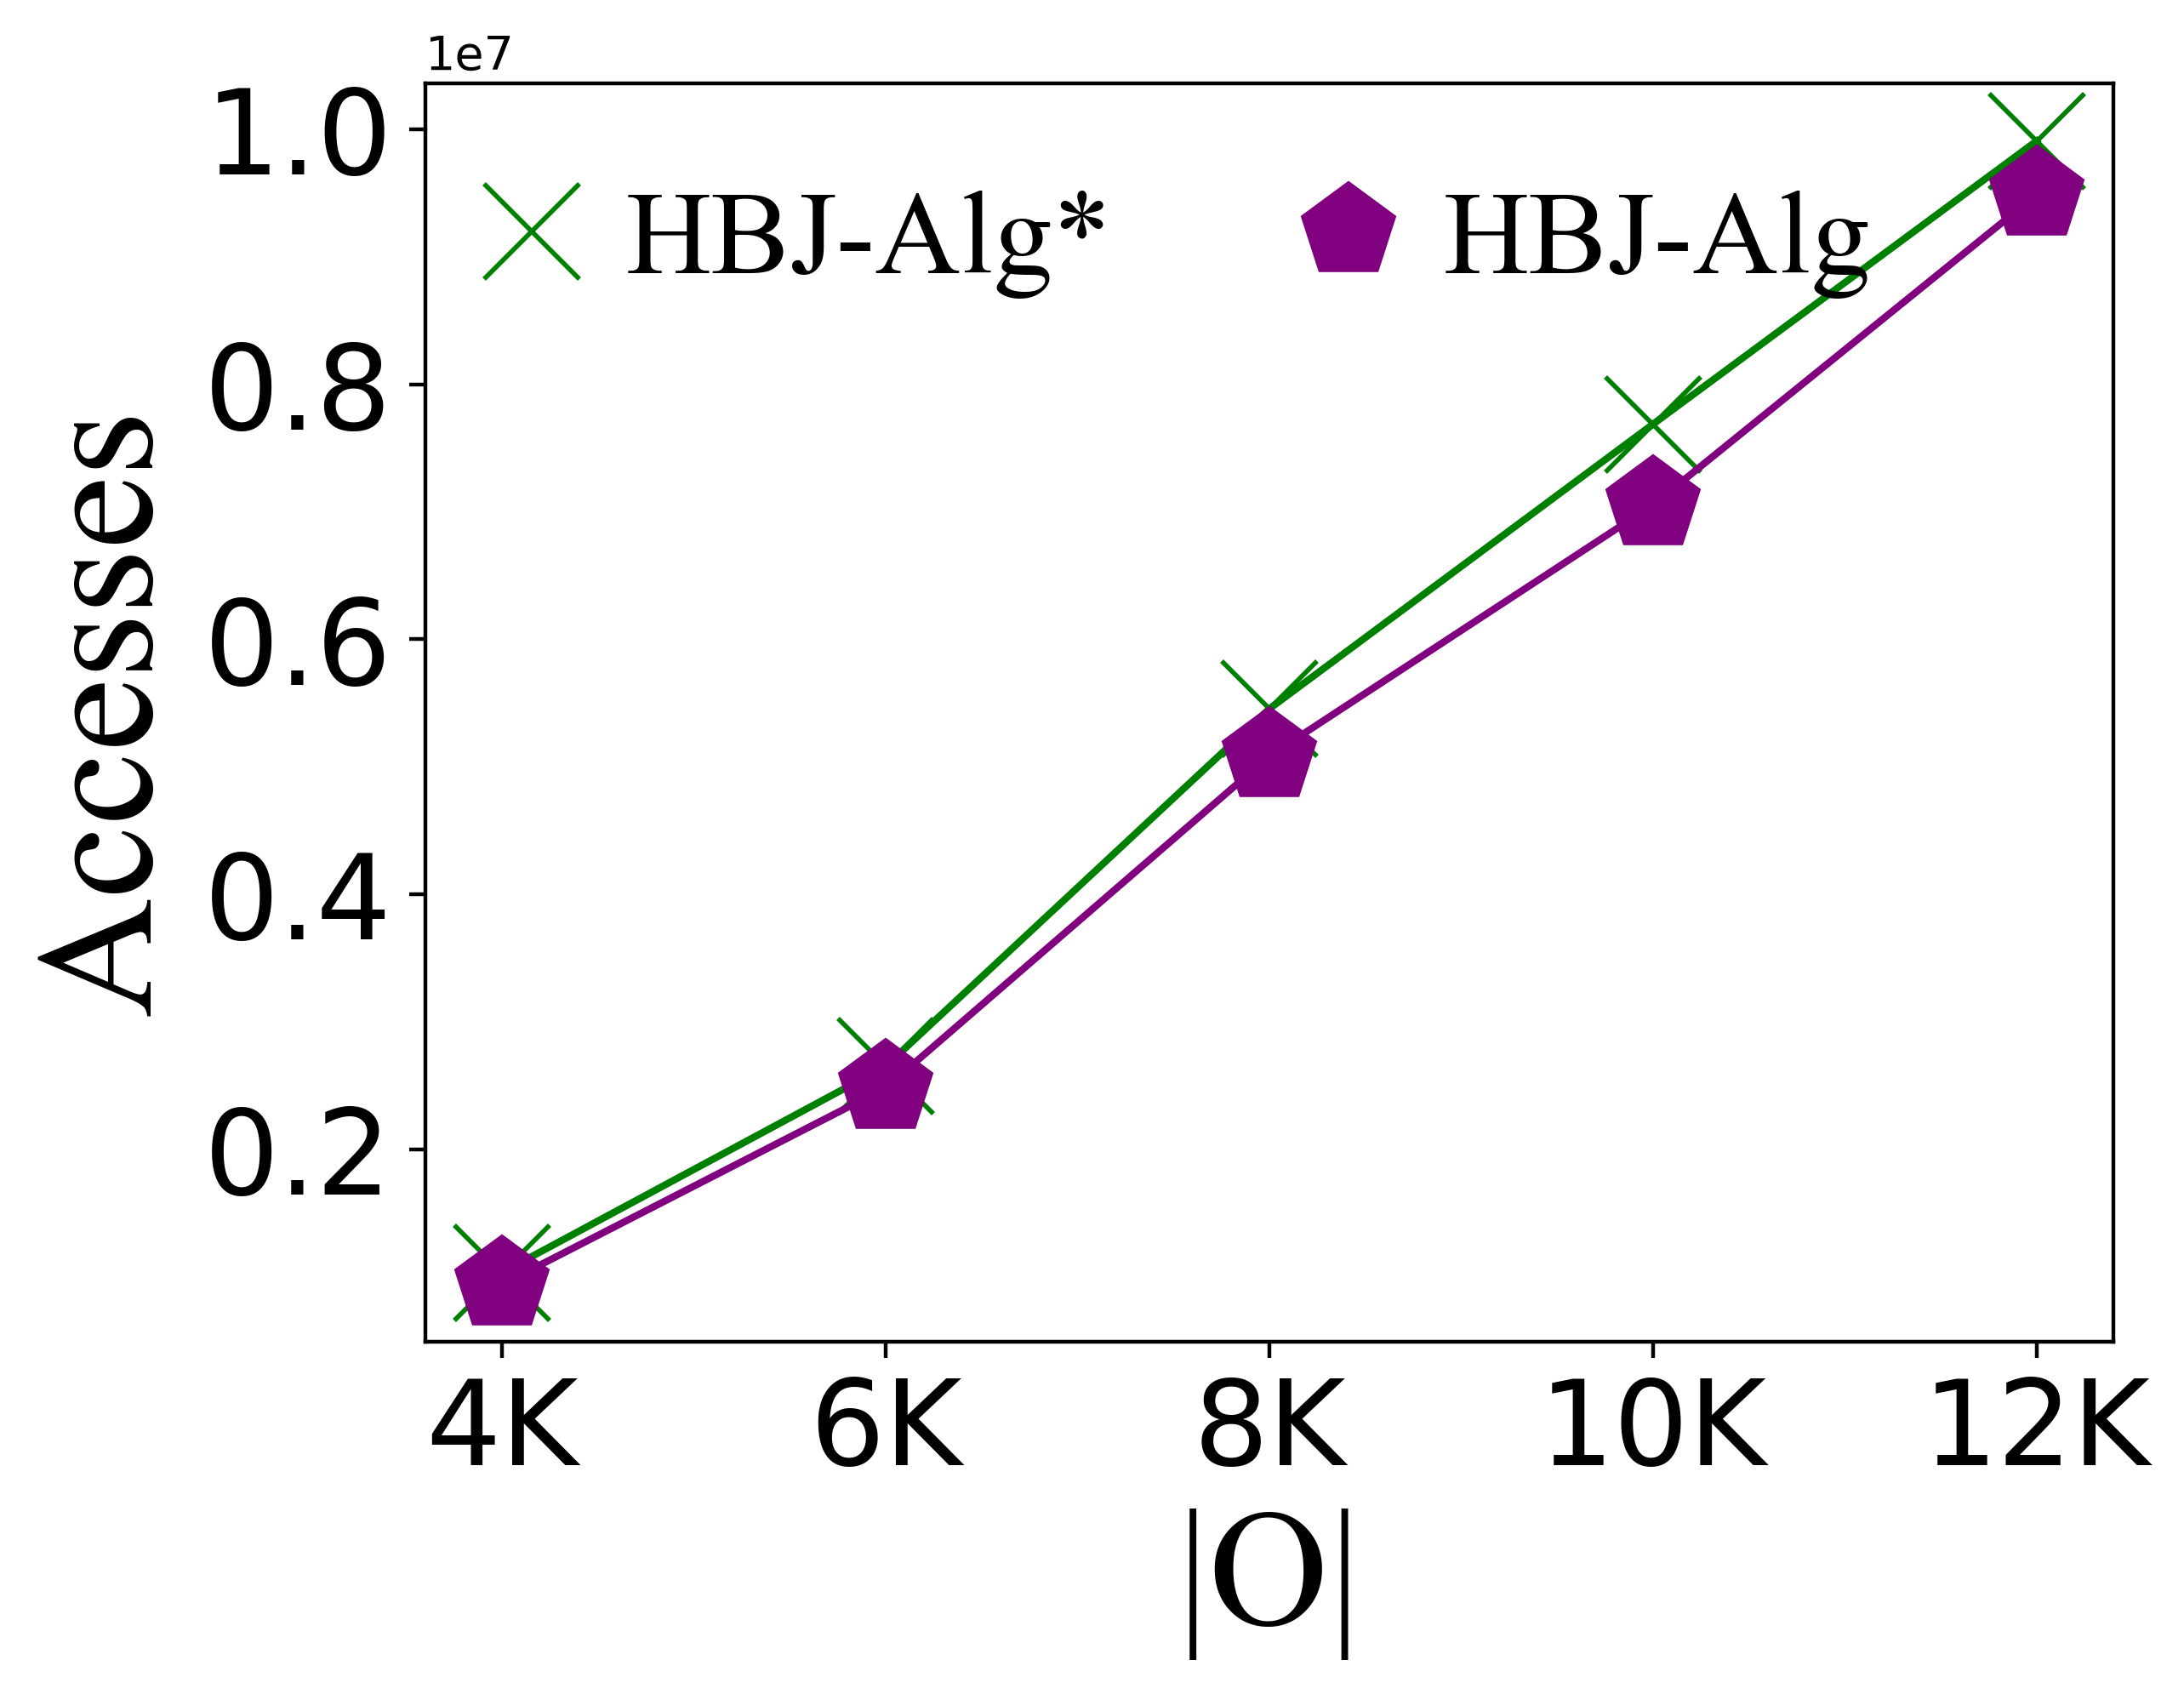
\includegraphics[width=0.4\textwidth]{fig/section6/geo-num-access.png}
        \label{geo-num-access}
    }%
    \hfill
    \subfloat[]{
        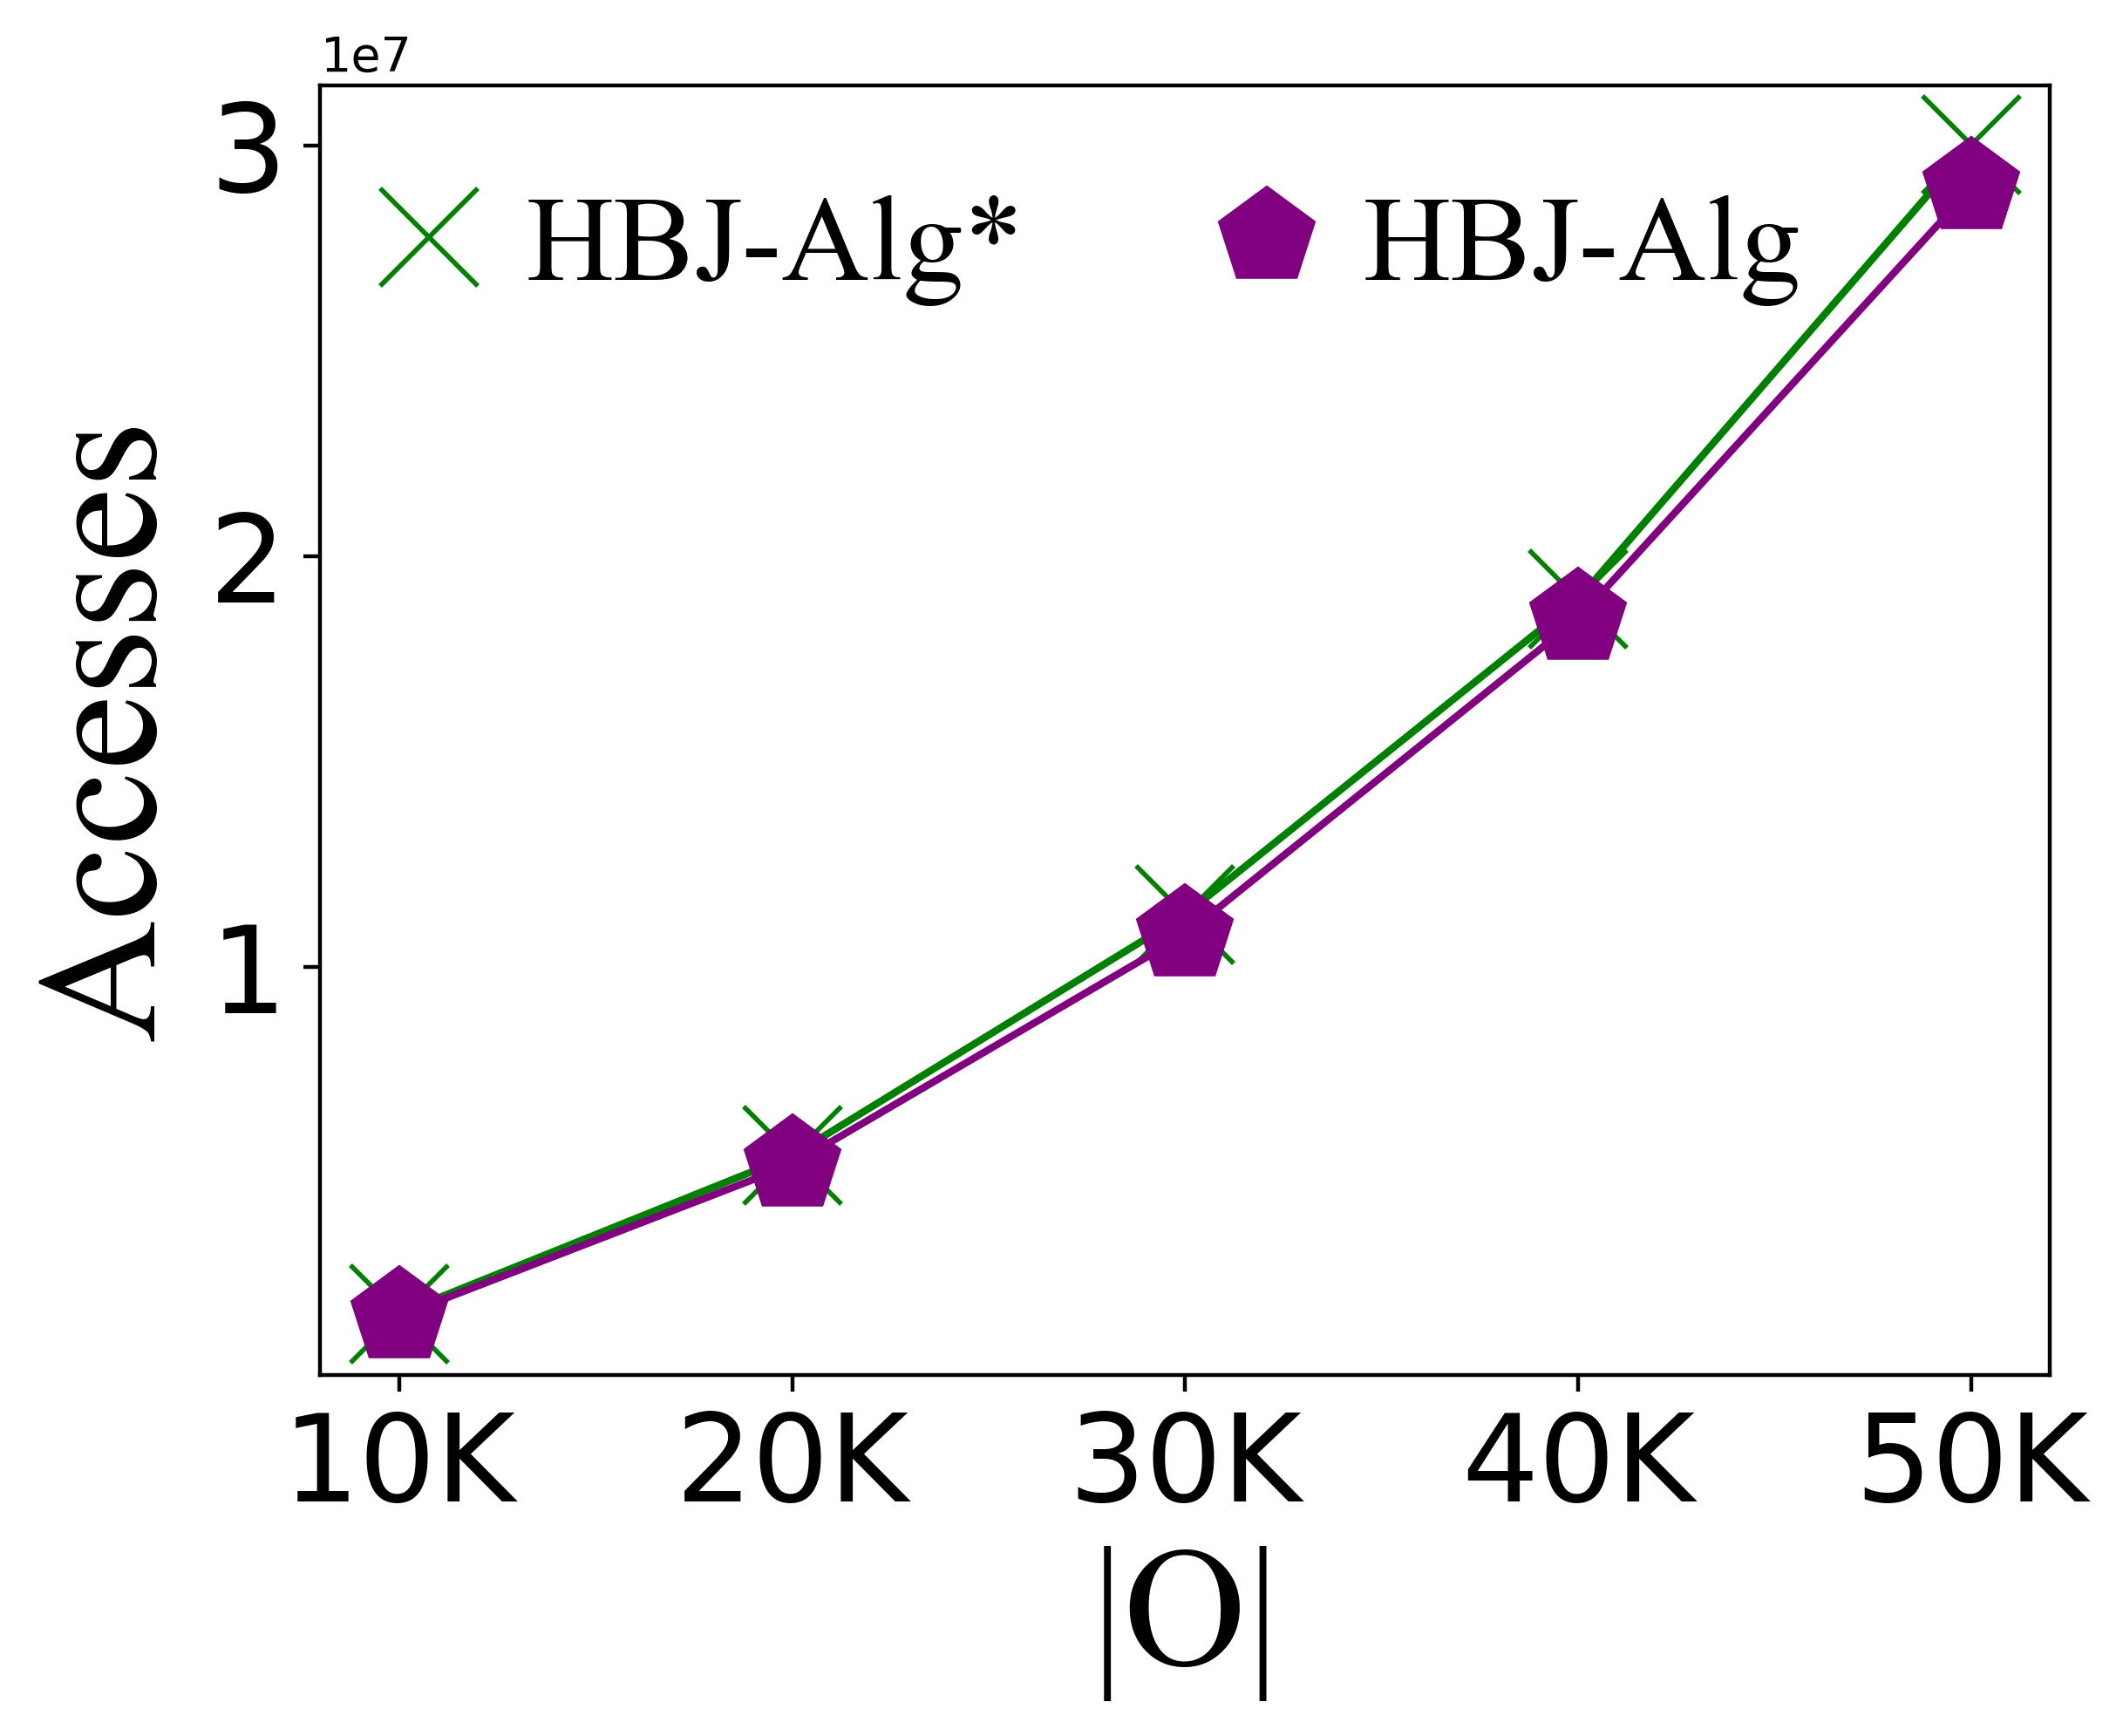
\includegraphics[width=0.4\textwidth]{fig/section6/pt-num-access.png}
        \label{pt-num-access}
    }%
    \caption{移动对象数量对节点访问次数的影响 \subref{geo-num-access}:Geolife数据集下的实验; \subref{pt-num-access}:Porto数据集下的实验}
    \label{img:vary_num_access}
\end{figure}

\subsection{Top-$k$ IS-Join 的实验研究}

\subsubsection{$k$ 的影响}
我们评估算法在 top-$k$ 交集相似度连接中的性能。图~\ref{img:vary_k_ftime} 展示了不同 $k$ 下的效率表现。可以看出，HBJ-Alg 在 Geolife 和 Porto 数据集上的 CPU 时间分别比 MBJ-Alg 提升约 3 倍和 5 倍。这表明我们的方法在 top-$k$ 连接中具有明显优势。

\begin{figure}[tb]
    \centering
    \subfloat[]{
        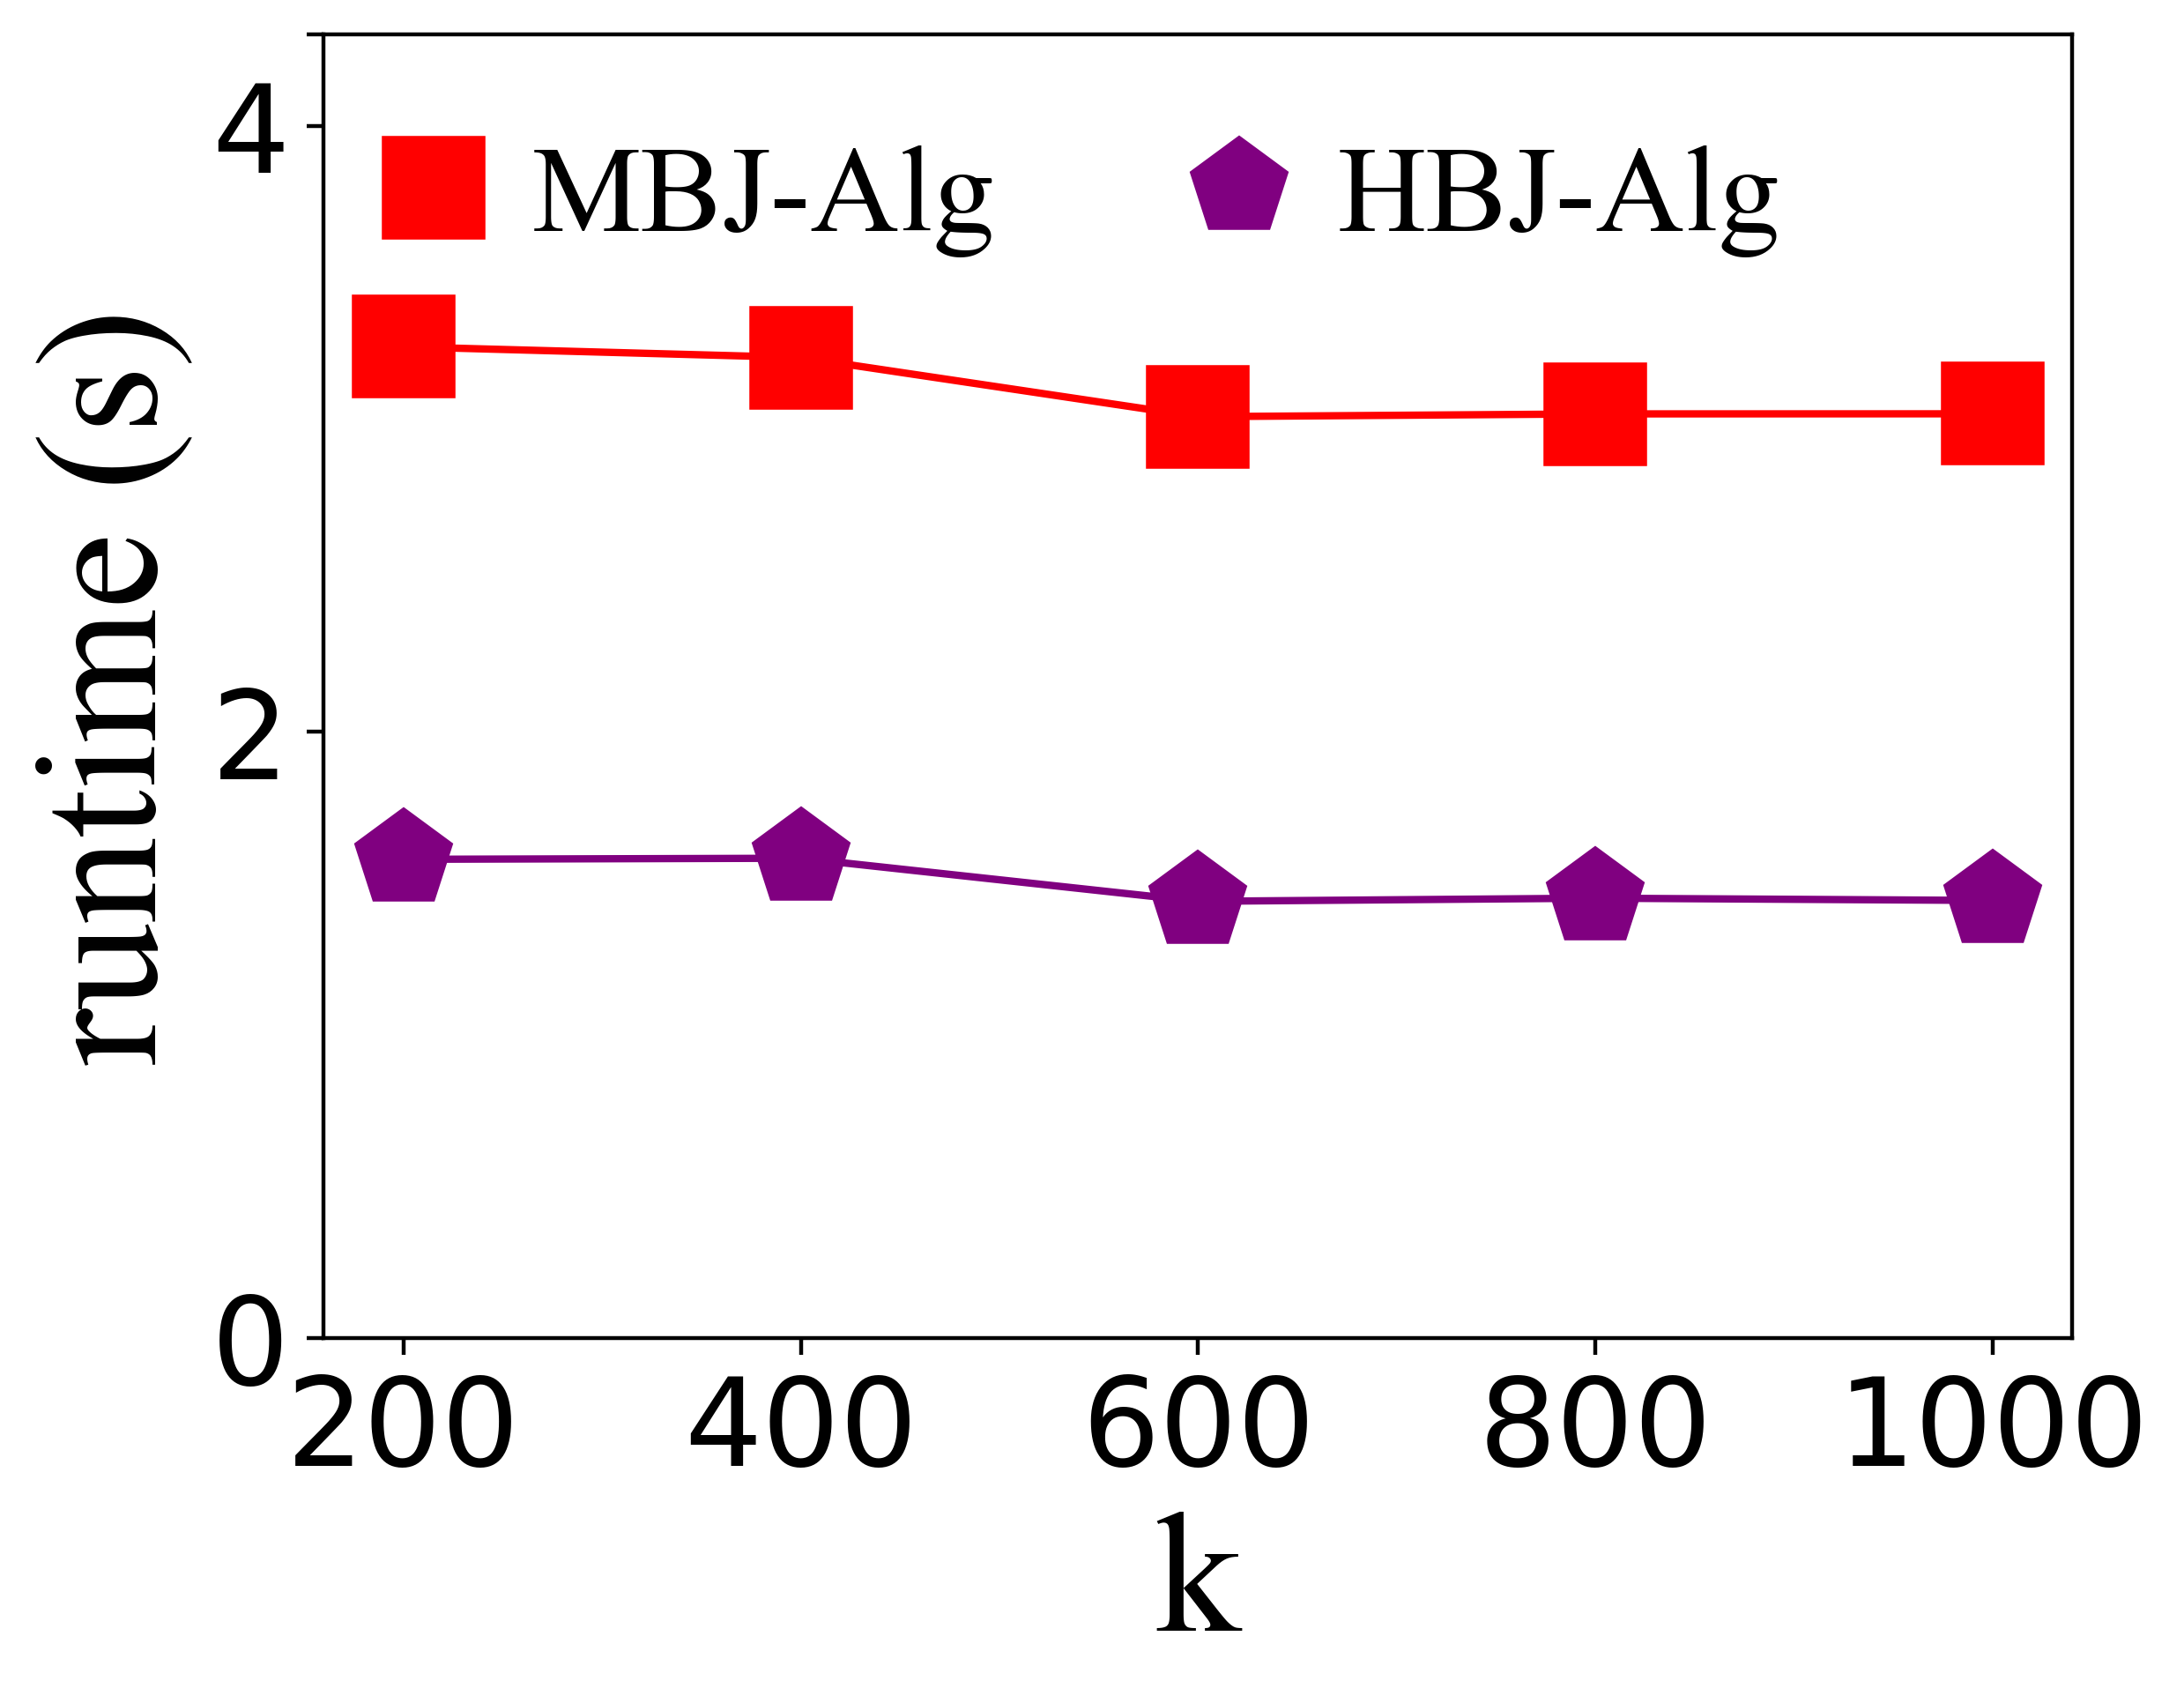
\includegraphics[width=0.4\textwidth]{fig/section6/geo-k-ftime.png}
        \label{geo-k-ftime}
    }%
    \hfill
    \subfloat[]{
        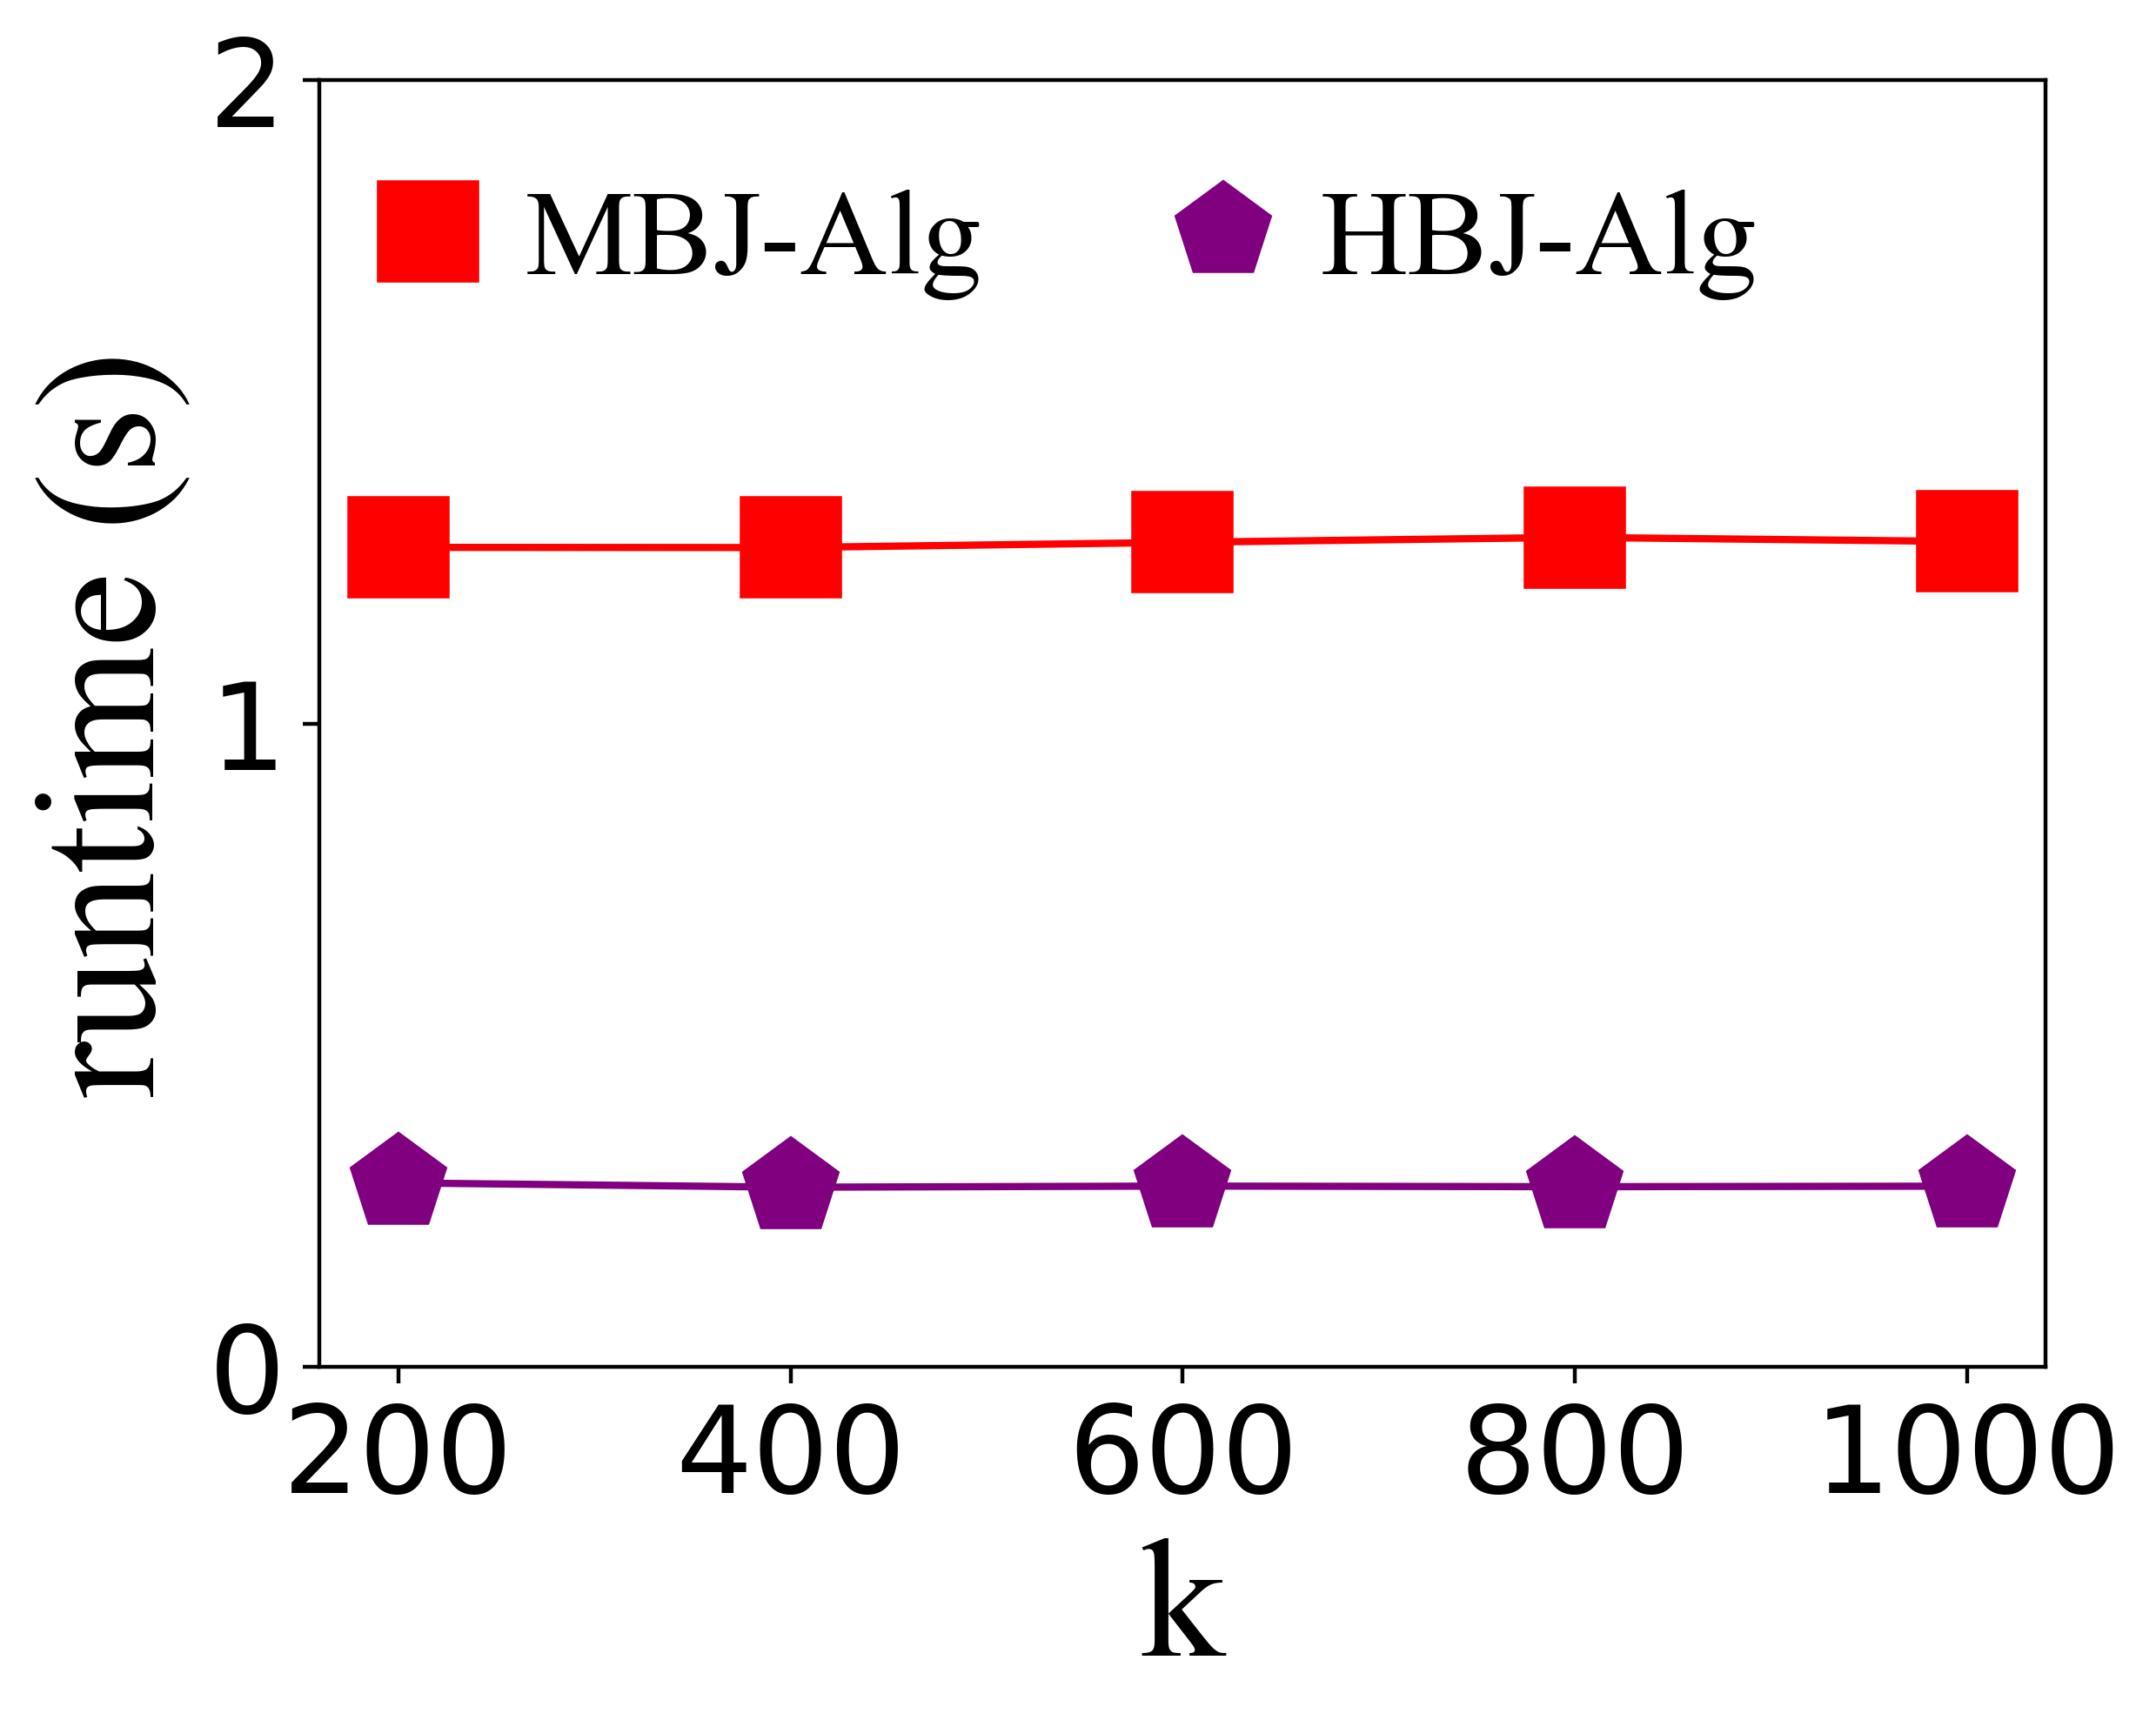
\includegraphics[width=0.4\textwidth]{fig/section6/pt-k-ftime.png}
        \label{pt-k-ftime}
    }%
    \caption{$k$ 的影响 \subref{geo-k-ftime}:Geolife数据集下的实验; \subref{pt-k-ftime}:Porto数据集下的实验}
    \label{img:vary_k_ftime}
\end{figure}

\section{特征精炼}

本节中，我们将时间点运动范围的特征视为面积。第~\ref{sec:refinement} 节介绍了对应的候选对象精炼方法，用于近似交集相似度计算。

\subsubsection{候选对象精炼}
\label{sec:refinement}

精确计算两个时间点运动范围的交集面积非常困难，计算代价高昂 \cite{DBLP:journals/comvis/HughesC12}。为了近似计算时间点交集相似度，我们在时间点运动范围内进行均匀采样。具体方法为，将运动范围包裹在矩形内，在矩形内均匀采样，再用椭圆方程过滤掉矩形外的点。一个更简洁的方法是极坐标采样 \cite{stark1979sampling}。  

具体做法如下：在 $MR(o,t_1)$ 上采样点，并计算落在 $MR(o',t_1)$ 内的点数量 $n_1$；在 $MR(o',t_1)$ 上采样点，并计算落在 $MR(o,t_1)$ 内的点数量 $n_2$。基于此，时间点交集相似度近似计算公式如下（记为 $IS'(o,o',t)$）：

\begin{equation}
    \label{eq:app point sim}
    IS'(o,o',t) = \frac{n_1}{|\mathcal{S}_o|} \times \frac{n_2}{|\mathcal{S}_{o'}|}
\end{equation}

其中，$|\mathcal{S}_o|$ 和 $|\mathcal{S}_{o'}|$ 分别表示对象 $o$ 和 $o'$ 的时间点运动范围的采样点数量。采样点数量与时间点运动范围面积成正比。采样点越多，近似结果越接近真实值，但计算开销也越大。

\begin{figure}[tb]
    \centering
    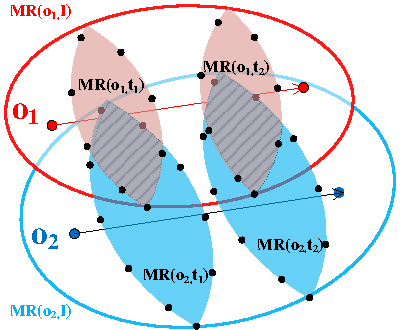
\includegraphics[width=0.6\textwidth]{fig/section6/sample.pdf}
    \caption{时间点运动范围内的采样示意}
    \label{fig:sample}
\end{figure}

\noindent
\textbf{示例. }
图~\ref{fig:sample} 展示了候选对象精炼的示例。假设候选集合 $\mathcal{L}=\{(o_1,o_2)\}$，其时间区间运动范围有交集。将当前时间区间划分为两个时间片 $t_1^\epsilon$ 和 $t_2^\epsilon$。在 $o_1$ 的时间点运动范围上采样 8 个点，在 $o_2$ 上采样 10 个点。  

在 $t_1$ 时，$n_1=3$，$n_2=2$，则根据公式~\ref{eq:app point sim}，$IS'(o,o',t_1)=\frac{3}{8}\times\frac{2}{10}=\frac{3}{40}$。在 $t_2$ 时，$IS'(o,o',t_2)=\frac{4}{8}\times\frac{2}{10}=\frac{1}{10}$。因此，$IS'(o,o',I,\epsilon)=(\frac{3}{40}+\frac{1}{10})/2=\frac{7}{80}$。

\section{本章小结}
本文提出了一种新的面向移动对象的运动范围感知相似连接框架 IS-Join。该框架通过引入对象的潜在运动区域，而非仅依赖离散的轨迹点，有效刻画了对象之间的时空交互关系。不同于传统的轨迹相似连接方法，IS-Join 以运动范围之间的交集相似度为建模对象，使其能够支持更加灵活的查询，适用于交通监控、野生动物追踪以及接触追踪等应用场景。为高效地在大规模数据上处理 IS-Join 查询，我们提出了一种融合重划分策略的 HBall-tree 索引结构，并设计了预检查与剪枝技术，以减少不必要的候选对象对评估，从而显著提升处理效率。基于两个真实世界数据集的大量实验结果表明，与精心设计的基线方法相比，我们的方法在性能上最高可获得约3倍的加速效果。
	% \chapter{总结与展望}

本章对全文进行总结，并分别列出每个研究内容的贡献创新，并讨论了未来可行的研究工作展望。
\section{全文总结}
随着 GPS 设备与智能移动终端的广泛普及，带有地理位置信息的时空数据呈现出爆炸式增长，这为城市计算与时空数据挖掘提供了丰富的数据基础，也带来了新的研究挑战。特别是在路径规划、接触搜索、联合移动模式挖掘以及轨迹相似性分析等任务中，如何在大规模、动态且存在观测不确定性的环境下进行高效计算，成为学术界和工业界亟需解决的问题。传统方法往往依赖离散轨迹点或静态路径集合，难以满足实时性、可扩展性及准确性要求，尤其在连续到达的行程请求流或大规模移动对象场景下，其性能和适用性存在明显局限。  为应对上述挑战，本文系统研究了面向城市计算的高效算法设计，提出了一系列针对不同场景与任务的算法框架。具体而言，本文涵盖四类核心研究工作：(1) 持续最优路径组合规划：针对动态路网中持续到达的行程请求流，提出了全局协同优化的路径规划方法，通过将时间窗口内的请求作为整体进行联合优化，实现整体通行效率的提升，有效缓解交通拥堵。  (2) 联合移动模式挖掘：面向大规模移动对象轨迹数据，设计了高效的群体模式检测算法，用于高效发现一种宽松的联合移动模式，支持交通管理、拼车推荐及异常行为识别等应用。 (3) 接触搜索与疾病传播分析：针对大规模连续轨迹数据，提出可扩展且低延迟的接触搜索方法，通过运动范围建模有效识别潜在接触事件，为公共卫生监测、疫情防控及风险评估提供数据支撑。  (4) 轨迹相似连接：提出基于运动范围的交集相似性连接框架，突破传统离散点方法的局限，在稀疏采样或不确定条件下仍能稳健刻画对象间潜在交互关系，适用于交通监控、野生动物迁徙分析及接触追踪等场景。  



\subsection{面向大规模行程请求流的持续最优路线组合规划} 
本文在\ref{cha:route search}研究了城市计算应用中面向大规模行程请求流的全局协同路径规划问题。该问题的复杂性在于：行程请求以数据流形式持续到达，早期规划结果会影响未来交通状态，不同行程路径通过共享路段形成复杂耦合关系，从而导致组合搜索空间呈指数级增长。传统单次最优路径规划方法无法应对这种持续性、动态性和全局耦合性的挑战，容易在局部最优决策叠加下形成新的拥堵热点。  

为此，设计了一种高效的自感知批处理解决方案，用于持续优化行程请求流中的路线组合。解决方案包含两个核心步骤：初始路径搜索与批量优化处理。初始路径搜索步骤为每批新到达的行程请求生成高质量的初始路径组合，以避免潜在交通拥堵；批量优化处理步骤则在初始组合基础上进一步优化所有路径，以最小化总通行时间并提升整体路网效率。   研究成果和贡献总结如下：  
\begin{itemize}
    \item 提出了一种新颖的持续最优路线组合问题模型，适用于城市交通流管理、实时路径规划及拥堵预防等多种应用场景。
    \item 设计了高效的自感知批处理算法及剪枝机制，实现对大规模行程请求流的实时优化，兼顾准确性与计算效率。 
    \item 验证了所提方法在真实路网数据上的表现，相较于基线方法展现出更高的性能和可扩展性，在总通行时间优化和实时处理能力上具有显著优势。
\end{itemize}


\subsection{基于轨迹数据的群体联合移动模式挖掘} 
本文在\ref{cha:comovement}研究了城市计算应用中面向大规模移动对象轨迹的联合移动模式挖掘问题。该问题的复杂性在于：轨迹数据规模庞大，移动对象随时间持续变化，联合移动模式需要在空间邻近性、时间持续性及群体规模约束下进行精确判定；同时，传统模式定义在时间上过于严格，导致候选生成与验证成本极高，尤其在实时或近实时应用场景中难以满足计算效率要求。此外，群体成员可能暂时离开群体并重新加入，历史数据与新到达轨迹间存在强动态依赖，使得模式挖掘具有高度动态性与组合耦合性。  

为此，设计了一种针对伴随群体的高效挖掘框架，包含两类核心算法：精确搜索算法（ES-ECMC）和社区感知的近似搜索算法（CS-ACMC）。ES-ECMC算法基于严格的时空约束判定机制，对候选对象对及群体进行精确验证，保证结果完备性与准确性，适用于离线或中小规模数据场景；CS-ACMC算法通过近似计算与结构化聚类方法压缩搜索空间，实现高效增量挖掘，满足实时或近实时应用需求。整体解决方案的步骤为：首先在近似联合移动对搜索阶段，通过网格划分将轨迹离散化，并快速估计对象间联合移动程度生成候选对；随后在社区感知群体发现阶段，将候选对构建为图结构并利用社区检测算法进行聚类，从而高效识别伴随群体。 研究成果和贡献总结如下：
\begin{itemize}
    \item 提出了伴随群体模式定义，兼顾空间邻近性、时间持续性与群体规模约束，并适应动态轨迹数据环境，具备广泛应用价值，包括交通监测、疫情防控及公共安全预警等场景。
    \item 设计了精确与近似两类算法（ES-ECMC与CS-ACMC），有效解决了准确性与效率之间的权衡问题。
    \item 验证了所提方法在用户可交互时间内高效发现伴随群体的能力，同时展示了在大规模数据环境下的可扩展性与实用性；
\end{itemize}  
总体而言，本章在理论与实践层面系统研究了伴随群体发现问题，提出了高
效、可扩展且具有应用价值的解决方案，为大规模动态轨迹数据环境下的群体行
为挖掘提供了新的研究方法与技术工具。


\subsection{大规模移动对象上的持续密切接触发现} 
本文在\ref{cha:contact}研究了城市计算应用中面向大规模动态移动对象的实时密切接触检测问题。该问题的复杂性在于：轨迹数据以持续流的形式到达，移动对象数量巨大且不断变化，同时需要在空间邻近性与时间持续性约束下实时识别潜在密切接触对象。此外，密切接触具有递归扩展特性，即新发现的接触对象将继续参与后续检测，导致传播链持续增长，增加了算法的计算复杂度与状态维护难度。在突发公共卫生事件或大型人群聚集场景下，若无法高效处理轨迹流，将难以及时识别关键接触节点，从而影响风险控制决策。  

为此，设计了一种针对持续密切接触搜索问题的高效解决方案。解决方案包含两类核心算法：精确实时搜索算法和近似实时搜索算法。精确实时搜索算法通过严格的空间与时间约束判定，对候选对象进行精确验证，保证检测结果的完备性与准确性；近似实时搜索算法在保证不漏检的前提下，通过首尾优先检查、跳跃检测及近似机制显著降低计算量，实现高效实时处理。整体解决方案的步骤为：首先对轨迹对象进行分组过滤，减少候选对象数量；随后基于距离上下界的预检查策略避免不必要的精确距离计算；最后在滑动时间窗口内维护对象间接触状态，实现持续更新与递归扩展。  研究成果和贡献总结如下： 
\begin{itemize}
    \item 定义了持续密切接触搜索问题，为流行病传播监测、公共卫生预警及风险追踪提供统一的数据处理框架，明确了递归扩展与实时更新特性。
    \item 设计了精确与近似两类实时处理算法，结合分组过滤、预检查及跳跃检测等优化策略，有效解决了准确性与效率之间的权衡难题。
    \item 验证了所提出方法具有良好的可扩展性与稳定性：在保证检测精度的同时，实现了大规模动态场景下的高效实时密切接触检测。
\end{itemize} 
总体而言，本章系统研究了持续密切接触搜索问题，提出了高效、可扩展且具
有应用价值的解决方案，为大规模流式轨迹数据环境下的实时疫情监控与风险管
理提供了新的技术方法与实践参考。

\subsection{面向时空运动范围的轨迹相似度连接} 
本文在\ref{cha:join}揭示了城市计算应用中移动对象相似性连接问题中的一个关键挑战——在稀疏采样条件下如何准确刻画对象间潜在交互关系。传统基于离散采样点的相似性度量方法在对象轨迹采样频率不足或存在观测缺失时容易低估真实相似性，导致潜在对象对被误剪枝。为解决这一问题，提出了交集相似性连接问题，通过引入“运动范围”概念，将对象在相邻观测样本之间可能到达的空间区域建模为运动范围，并基于这些区域的交集程度进行相似性度量，从而在稀疏采样或数据噪声条件下更稳健地刻画潜在交互。

交集相似性连接问题在多个实际场景中具有重要应用价值。例如，在城市交通监测中，车辆轨迹的运动范围可映射为道路子路段或交叉口集合，通过交集相似性识别潜在交通关联，有助于拥堵预测与异常路段识别；在野生动物迁徙分析中，运动范围结合栖息地与迁徙通道信息，可识别共享走廊或高频活动区域，实现低采样频率下的关键交互检测；在公共卫生领域，个体潜在接触事件可通过运动范围交集推断，从而支持疾病传播建模与风险评估。不同应用虽对象类型与特征不同，但核心需求均为在观测不确定条件下识别潜在运动交集关系，该研究提供了统一且可扩展的解决框架。

在建模与计算上具有以下关键创新：首先，明确将相似性度量从离散点级距离扩展到连续时间下的区域交集，允许在理论上处理未观测时间段的潜在交互；其次，将连续时间区间内的交集相似性定义为时间平均函数，既保留连续性信息，又便于离散化近似计算。该建模显著提升了稀疏采样条件下潜在对象对识别能力，同时引入连续时间处理与大规模候选对计算的两大挑战：一是连续时间计算的复杂性，需设计可计算的离散化或可控近似方法；二是高效连接的挑战，现有点或静态区域相似性算法无法直接支持连续时间运动范围的交集计算，否则候选对象对数量会急剧膨胀。

为应对上述挑战，提出了基于时间区间运动范围的高效求解框架。核心思想是通过混合 球树索引对对象运动范围进行层次化组织，并结合重划分策略与多级剪枝技术，有效过滤候选对象对，从而在保证正确性与完整性的前提下显著降低计算开销。该框架适用于稀疏采样轨迹数据，能够高效识别满足相似性阈值的对象对，实现连续时间区间下的交集相似性计算。研究成果和贡献总结如下：  
\begin{itemize}
    \item 提出了交集相似性连接问题，将相似性度量从离散点扩展到连续时间下的运动范围交集，显著增强稀疏采样轨迹潜在交互建模能力。
    \item 构建了混合球树层次索引结构，并结合重划分与多级剪枝策略，实现大规模连续时间区间下的高效连接计算。
    \item 验证了所提出方法的可扩展性与实用价值：结果表明方法在保证准确性的前提下，相较于现有基线方法平均运行时间降低约 3 倍。
\end{itemize}

总之，本文针对稀疏采样轨迹数据中潜在运动交集关系的识别提出了统一建模与高效计算框架，为交通分析、生态监测及公共卫生等多种实际场景提供了可行且高效的技术方案。

\section{展望}
本文针对城市计算应用中的4个需求，即面向大规模行程请求流的持续最优路线组合规划需求，基于轨迹数据的群体联合移动模式挖掘需求，面向大规模移动对象的持续密切接触查询需求，以及面向时空运动范围的轨迹相似度连接需求展开了深入研究，发表了一系列研究成果，但仍存在一些值得进一步研究和探索的空间。随着移动对象数据规模和实时更新频率的持续增长，单机处理在计算能力与内存资源上面临显著瓶颈。未来可能的进一步研究方向可以向分布式环境、深度学习优化、时空大模型拓展，潜在研究方向包括：

\paragraph{分布式查询}
针对大规模移动对象或位置标注数据，当数据量超出单机处理能力时，可在分布式框架中研究并行化的索引机制和查询算法。研究重点可包括：面向海量时空-文本数据的并行查询架构，优化任务调度与负载均衡；以及分布式数据迁移与副本管理策略，以保证连续查询过程中的数据一致性与高可用性。在分布式环境下，将交集相似性连接或连续密切接触搜索等计算任务进行分片处理，同时保持跨节点候选对象的完整性与准确性，是提高系统可扩展性与实时性的重要方向。相关研究可包括分布式滑动窗口维护、跨节点运动范围交集计算以及并行剪枝策略设计。分布式处理环境中，节点故障、网络延迟及数据倾斜可能导致查询性能下降。未来可探索自适应任务调度、容错恢复机制以及数据划分优化方法，以保障大规模连续时空查询的稳定性与效率。

\paragraph{基于深度学习的方法优化}
随着移动对象数据的持续增长与复杂化，传统基于规则或索引的算法在处理大规模、动态、多源数据时面临性能和可扩展性瓶颈。深度学习技术因其强大的表示学习和模式捕捉能力，为未来时空数据分析与连续查询提供了新的研究契机。具体而言，潜在的研究方向可包括以下几个方面：（1）在大规模行程请求流场景下，如何为海量移动对象实时生成最优路线组合是关键问题。深度强化学习可用于建模连续决策过程，将路线选择、时间窗口约束和交通动态因素作为状态与奖励函数，实现高效、可扩展的路径优化。通过结合历史轨迹数据与实时交通信息，模型可学习群体行程模式，从而在动态环境中提供持续优化的路线方案。（2）群体行为分析和联合移动模式识别在城市规划、公共交通调度及疫情传播监控中具有重要意义。深度学习方法，如图神经网络或时空卷积网络，可以将移动对象及其轨迹视为时空图结构或序列数据，从而自动捕捉潜在的群体协同行为、同步移动模式及关键影响节点，实现对复杂群体行为的高效挖掘。（3）持续密切接触检测涉及大规模对象在动态环境下的空间邻近与时间连续性判定。深度学习模型可通过学习对象轨迹的潜在运动分布和邻近概率，实现对未观测时间段潜在接触的预测，从而在海量数据流环境下支持实时、鲁棒的密切接触检测。结合序列建模与空间嵌入方法，可以有效提升接触预测的精度与响应速度。（4） 在稀疏采样轨迹或不完整数据条件下，基于传统规则的运动范围交集计算容易受限。深度表示学习可通过将轨迹映射到低维时空潜在空间，捕捉连续时间区间内的潜在重叠关系，从而高效完成交集相似性连接。此外，生成式模型可以辅助补全未观测轨迹，进一步增强相似性连接的准确性与鲁棒性。

\paragraph{时空大模型设计}
未来可以构建一个统一的时空大模型框架，将轨迹数据分析、群体联合移动模式挖掘、持续密切接触查询以及轨迹相似度连接等任务整合在同一平台中，并提出接口用于用户交互。该框架可通过深度学习方法实现统一时空表示，将多源轨迹、行为和环境信息映射到低维潜在空间，从而支持个体轨迹预测、群体模式识别、实时接触检测和交集相似性计算。针对大规模和高频数据，可在分布式计算环境下进行流式处理与增量模型更新，实现高效并行计算与实时响应。同时，框架可提供统一接口与查询语义，便于不同应用场景快速接入，包括智能交通、公共卫生监控和生态保护等。结合可解释性和隐私保护技术，系统既能输出可理解的决策依据，又保障个体数据安全。整体来看，该统一时空大模型有望通过深度学习和大数据优化，实现跨任务、跨数据源的高效、实时和可扩展时空智能分析。

	\chapter{后截断章节} %删除前检查是否存在后截断章节

	\acknowledgement
	本研究及学位论文是在我的导师商烁教授的亲切关怀和悉心指导下完成的。他严肃的科学态度，严谨的治学精神，精益求精的工作作风，深深地感染和激励着我。老师不仅在学业上给我以精心指导，同时还在思想、生活上给我以无微不至的关怀，在此谨向商烁教授致以诚挚的谢意和崇高的敬意。
    
感谢我的副导师吴刚副教授。吴老师在我攻博期间的科研道路中给予了我极大的帮助，每当遇到科研难题，吴老师都会为我提供正确的思路，并且耐心帮助我解决许多实际问题。在投稿学术论文和撰写博士学位论文的过程中，吴老师都帮助我进行了细致的审阅和修改，使我的科研内容顺利完成。

攻读博士学习时光已经接近尾声，在此我想对我的母校，我的父母、亲人们，我的老师和同学们表达我由衷的谢意。感谢东北大学的老师和同门的关心和鼓励。老师们课堂上的激情洋溢，课堂下的谆谆教诲；同学们在学习中的认真热情，生活上的热心主动，所有这些都让我的七年充满了感动。这次毕业论文设计我得到了很多老师和同学的帮助，其中我的论文指导老师王国仁老师对我的关心和支持尤为重要。王国仁老师不仅在学业上给我以精心指导，同时还在思想给我以无微不至的关怀，在此谨向王国仁老师致以诚挚的谢意和崇高的敬意。同时，本篇毕业论文的写作也得到了实验室的等老师的热情帮助。我要感谢和我在一个小组里并肩作战,共同学习的同学们,感谢李，以及实验室其他师姐师兄和师弟师妹和曾经在各个方面给予过我帮助的伙伴们，在此，我再一次真诚地向帮助过我的老师和同学表示感谢！

感谢培养教育我的学校，浓厚的学术氛围，舒适的学习环境我将终生难忘！祝母校蒸蒸日上，永创辉煌！感谢对我倾囊赐教、鞭策鼓励的东北大学诸位师长，诸位恩师的谆谆训诲我将铭记在心。祝恩师们身体健康，家庭幸福！感谢论文中引文的原作者，他们都是计算机界的名师大家，大师风范，高山仰止。祝他们寿域无疆，德业永辉！感谢同窗好友以及更多我无法逐一列出名字的朋友，他们和我共同度过了七年美好难忘的大学时光，我非常珍视和他们的友谊！祝他们前程似锦，事业有成！最后，我要感谢我的父母和亲人，无论我面对任何失败和挫折，你们都给予我最体贴的关怀和安慰，让我感受到家永远都是我最坚实的后盾，我才能无所畏惧的一路向前。你们坚定的支持给予我无限的动力，使我能够克服和战胜生活路上的艰难险阻，在人生路上不断前行。今后，我会用自己不懈的努力来回报你们的恩情。感谢生活中众多给了我鼓励和帮助的亲朋好友，我在这里无法一一列出他们的名字，但是他们对我的恩情我永远不会忘记，在这里写下我对他们的感激。

	%% 参考文献部分
	\nocite{*}% 为了便于在示例文档中展示参考文献而设，正式撰写时需要注释掉
	% \bibliographystyle{DissertUESTC}% 自v25.03.12版本后，参考文献风格文件由用户设定的论文类型选项自动确定，无需在此手动设置
	\bibliography{ref}

	% 
% 附录起始位置
\appendix

\chapter{九阴真经原本}

\section{总纲（核心心法）}

\subsection{梵文总纲（后由郭靖、黄蓉译解）：}

原版《九阴真经》的总纲以梵文写成，蕴含武学至高哲理，强调“阴阳互济、刚柔并重”，是化解经中武功戾气的关键。

关键理念：“天之道，损有余而补不足”（出自《道德经》），主张内力修炼需顺应自然，调和阴阳。


\chapter{黯然销魂掌秘籍}

\section{黯然销魂掌的来历}

\subsection{创招背景：}

杨过与小龙女分离十六年，饱受相思之苦，内心极度悲怆。

在南海之滨练剑时，结合毕生所学，创出这套以情驭劲的掌法。

\subsection{武学根基：}

融合《九阴真经》的刚柔并济、古墓派的轻灵迅捷、欧阳锋的蛤蟆功爆发力、黄药师的弹指神通巧劲，以及洪七公的打狗棒法变化。

\section{黯然销魂掌的十七式}

\begin{table}[!h]
    \caption{黯然销魂掌招式解析}
    \begin{tabular}{l l}
        \toprule
        \textbf{招式} & \textbf{要领} \\
        \midrule
        拖泥带水 & 缠绵悱恻，掌力如浪潮般连绵不绝 \\
        孤形只影 & 身形飘忽，掌劲忽左忽右，难以捉摸 \\
        心惊肉跳 & 以极快掌法扰乱对手心神，使其胆寒 \\
        徘徊空谷 & 掌力回荡，如幽谷回声，劲力反复叠加 \\
        力不从心 & 看似无力，实则暗藏后劲，后发制人 \\
        行尸走肉 & 身法诡异，如僵尸般飘忽不定 \\
        庸人自扰 & 掌势混乱无序，却暗合武学至理 \\
        饮恨吞声 & 掌力内敛，蓄势待发，一击必杀 \\
        六神不安 & 掌风笼罩对手全身，使其难以招架 \\
        穷途末路 & 绝境反击，掌力爆发至极限 \\
        面无人色 & 掌风阴寒，令对手如坠冰窟 \\
        想入非非 & 虚招惑敌，实则暗藏杀机 \\
        呆若木鸡 & 静立不动，却蕴含极强防御反击之势 \\
        神不守舍 & 掌法飘忽，如鬼魅般难以预测 \\
        魂不附体 & 掌劲透体，直击对手经脉 \\
        倒行逆施 & 逆反常理，出招角度刁钻 \\
        黯然销魂 & 终极杀招，需极度悲痛心境才能施展 \\
        \bottomrule
    \end{tabular}
\end{table}

\section{黯然销魂掌的特点}
	% \achievement % 仅研究生用

	\section*{发表论文：}
	
	\begin{enumerate}
		\item \textbf{Li Ke}, Leong Hou U, Shang Shuo. App2Exa: accelerating exact kNN search via dynamic cache-guided approximation. International Joint Conferences on Artificial Intelligence, 2025: 3045-3053. %(\textbf{CCF A}, \underline{中科院分区}, IF: 98.8)
		
		\item \textbf{Li Ke}, Chen Lisi, Shang Shuo, Christian S Jensen, Panos Kalnis. Beyond Locations: A Motion Range-Aware Similarity Join. In Proceedings of the 31st ACM SIGKDD Conference on Knowledge Discovery and Data Mining V. 2, 2025:  1424-1434. %(\textbf{CCF A}, \underline{中科院分区}, IF: 98.8)
		
		\item Ding Zhongjun, \textbf{Li Ke}, Chen Lisi, Shang Shuo. Parallel online similarity join over trajectory streams. Proceedings of the ACM on Web Conference, 2025: 3426-3437. %(\textbf{CCF A}, \underline{中科院分区}, IF: 98.8)
		
		\item Chen Ziwen, \textbf{Li Ke}, Zhou Silin, Chen Lisi, Shang Shuo. Towards robust trajectory similarity computation: Representation-based spatio-temporal similarity quantification. World Wide Web, 2023, 26(4): 1271-1294. %(\textbf{CCF A}, \underline{中科院分区}, IF: 98.8)
		
		\item \textbf{Li Ke}, Chen Lisi, Shang Shuo, Wang Haiyan, Liu Yang, Panos Kalnis, Bin Yao. Towards Controlling the Transmission of Diseases: Continuous Exposure Discovery over Massive-Scale Moving Objects. International Joint Conferences on Artificial Intelligence, 2022: 3891-3897. %(\textbf{CCF A}, \underline{中科院分区}, IF: 98.8)
		
	    \item \textbf{Li Ke}, Chen Lisi, Shang Shuo. Towards alleviating traffic congestion: Optimal route planning for massive-scale trips. International Joint Conferences on Artificial Intelligence, 2021: 3400-3406. %(\textbf{CCF A}, \underline{中科院分区}, IF: 98.8)
	    
		\item \textbf{Li Ke}, Chen Lisi, Shang Shuo, Panos Kalnis, Bin Yao. Traffic congestion alleviation over dynamic road networks: Continuous optimal route combination for trip query streams. International Joint Conferences on Artificial Intelligence, 2021, 62(10): 5344--5348. %(\textbf{CCF A}, \underline{中科院分区}, IF: 98.8)
		
		
		
		\item Wang Hongyu, \textbf{Li Ke}, Shang Shuo. DLRD: dual-level network for rumor detection on geo-textual data. GeoInformatica, 2024, 28 (2): 335-351. %(\textbf{CCF A}, \underline{中科院分区}, IF: 98.8)
		
		\item Chen Ziwen, \textbf{Li Ke}, Chen Lisi, Hu Nan, Yoshiharu Ishikawa. Co-movement aware trajectory generation via waypoint-guided generative adversarial networks. GeoInformatica, 2025, 29 (4): 1093-1119. %(\textbf{CCF A}, \underline{中科院分区}, IF: 98.8)
		
		\item Chen Ziwen, \textbf{Li Ke}, Yoshiharu Ishikawa. Ca-gen: Trajectory generation with co-movement awareness. Proceedings of the 19th International Symposium on Spatial and Temporal Data, 2025: 115-118. %(\textbf{CCF A}, \underline{中科院分区}, IF: 98.8)

		\item \textbf{Li Ke}, Rao Xuan, Pang Xiaobing, Chen Lisi, Fan Siqi. Route search and planning: A survey. Big data research, 2021, 26: 100246. %(\textbf{CCF A}, \underline{中科院分区}, IF: 98.8)
		
        
        \item \textbf{Li Ke}, Wang Hongyu, Chen Ziwen, Chen Lisi. Relaxed group pattern detection over massive-scale trajectories. Future Generation Computer Systems, 2023, 144: 131-139. %(\textbf{CCF A}, \underline{中科院分区}, IF: 98.8)
        
		\item Wang Chenhao, \textbf{Li Ke}, Chen Lisi. Deep unified attention-based sequence modeling for online anomalous trajectory detection. Future Generation Computer Systems, 2023, 144: 1-11. %(\textbf{CCF A}, \underline{中科院分区}, IF: 98.8)
		
		\item Wang Haiyan, Feng Jiaming, \textbf{Li Ke}, Chen Lisi. Deep understanding of big geospatial data for self-driving: Data, technologies, and systems. Future Generation Computer Systems, 2022, 137: 146-163. %(\textbf{CCF A}, \underline{中科院分区}, IF: 98.8)

		
		
		
		
		


	\end{enumerate}
	
	\newpage
	% %%%%%% 开启“外文资料原文”
	%% \originalliterature{<外文标题>}{<外文作者>}
	\originalliterature{How to Take Revenge When My Father's
	Murderer is Suspected to Be a Famous Hero}{Yang Guo}

	%% 这部分内容务必使用模板提供的首字母大写的标题命令生成对应的外文原文标题，
	%% 否则，对应内容将出现在正文的目录和pdf的书签中，非常冗余。
	%% 另外，可使用的各级标题有\Section{}、\Subsection{}、\Subsubsection{}，没有chapter

	\textit{Abstract}——When Yang was a teenager, his mother contracted a disease and died, and he then lived a wandering life. When he met Guo Jing and his wife, they took care of him. However, due to the conflict between Yang and Guo Fu, Guo Jing sent him to learn martial arts in the Quanzhen Sect.

	\textit{Index Terms}——Martial arts, apostasy, revenge, fighting against the enemy, martial arts, apostasy, revenge, fighting against the enemy

	\Section{Introduction}

	\begin{table}[htp]
		\captionsetup{list=no}% 阻止此表格显示在表目录中
		\caption{Example of a table}
		\begin{tabular}{ccccc}
			\toprule
			\multirow{2}{*}{Column0} &  \multicolumn{2}{c}{Column1\tnote{1}} & \multicolumn{2}{c}{Column2\tnote{2}} \\
			\cmidrule(lr){2-3}\cmidrule(l){4-5}
			~     & subcolumn1 & subcolumn2 & subcolumn1 & subcolumn2 \\
			\midrule
			Row1  & element11 & element12 &element13 & element14 \\
			Row2  & element21 & element22 &element23 & element24 \\
			\cmidrule{2-3}\cmidrule{4-5}
			Row3  & element31 & element32 &element33 & element34 \\
			\bottomrule
		\end{tabular}
	\end{table}


	\Subsection{Contributions}


	\Subsubsection{While while while}

	\begin{longtable}{p{2em} p{6em}}
		\captionsetup{list=no}% 阻止此表格显示在表目录中
		\caption{Recommended journals and conferences}\\
		
		\toprule
		\textbf{Num} & \textbf{Abbreviation} \\
		\midrule
		\endfirsthead
		
		% 在这里设计首页以外的表题和表头
		\CPcaption{2}{Recommended journals and conferences}\\
		\toprule
		\textbf{Num} & \textbf{Abbreviation} \\
		\midrule
		\endhead
		
		% 在这里设计首页以外的表尾
		\bottomrule
		\multicolumn{2}{l}{to next page} \\  % 如不希望跨页表尾显示任何内容则注释掉即可
		\endfoot
		
		\bottomrule
		\endlastfoot
		
		1 & JSAC \\
		2 & TMC \\
		3 & TON \\
	\end{longtable}
	
	\Section{Related works}

	
	\Section{System model}

	%% 在“外文资料原文”部分，排版定义、公理、定理、命题、推论、引理、示例、假设需使用对应首字母大写的环境，如下所示

	
	\Section{Algorithm design}

	\begin{algo}[!h](8em)
		\caption{Example of an algorithm}
		\Input{1) input1; 2) input2.}
		\Output{result.}

		Pseudocode line 1.
		
		\For(\tcc*[f]{for note 1}){Condition 1}{
			Pseudocode line 2.
			
			\tcp{note 2}
			Pseudocode line 3.
			
			\DoWhile(\tcc*[f]{while note 3}){Condition 2}{
				Pseudocode line 4.
			}
			
			\tcc{loop cycle}
			\Loop(\tcc*[f]{note 4}){
				cycle body 1.
			}
			
			\Repeat(\tcc*[f]{repeat note 5}){Condition 3}{
				cycle body 2.
			}
			\eIf(\tcc*[f]{if note 6}){Condition 6}{
				when true，Pseudocode line 5.
			}{
				when false，Pseudocode line 6.\tcp*[f]{repeat cycle}
			}
		}
		\textbf{return} result.
	\end{algo}
	
	\Section{Experiments}

	
	\Section{Conclusions}
	% %%%%%% 开启“外文资料译文”
%% \translatedliterature{<译文标题>}{<原文作者>}
\translatedliterature{关于我的杀父仇人疑似是名震天下的
	大侠时该如何报仇}{杨过}

	%% 这部分内容务必使用模板提供的首字母大写的标题命令生成对应的外文译文标题，
	%% 否则，对应内容将出现在正文的目录和pdf的书签中，非常冗余。
	%% 另外，可使用的各级标题有\Section{}、\Subsection{}、\Subsubsection{}，没有chapter

	\textit{摘要}——杨过少年时期母亲染病而亡

	\textit{关键词}——练武，离经叛道，复仇，抗敌，练武，离经叛道，复仇，抗敌，练武，离经叛道，复仇，抗敌，练武，离经叛道，复仇，抗敌

	\Section{引言}

	\begin{table}[htbp]
		\captionsetup{list=no}% 阻止此表格显示在表目录中
		\caption{表格样例}
		\begin{tabular}{ccccc}
			\toprule
			\multirow{2}{*}{Column0} &  \multicolumn{2}{c}{Column1\tnote{1}} & \multicolumn{2}{c}{Column2\tnote{2}} \\
			\cmidrule(lr){2-3}\cmidrule(l){4-5}
			~     & subcolumn1 & subcolumn2 & subcolumn1 & subcolumn2 \\
			\midrule
			Row1  & element11 & element12 &element13 & element14 \\
			Row2  & element21 & element22 &element23 & element24 \\
			\cmidrule{2-3}\cmidrule{4-5}
			Row3  & element31 & element32 &element33 & element34 \\
			\bottomrule
		\end{tabular}
	\end{table}


	\Subsection{贡献}


	\Subsubsection{好好好}

	\begin{longtable}{p{2em} p{4.5em}}
		\captionsetup{list=no}% 阻止此表格显示在表目录中
		\caption{中科院部分推荐期刊及会议}\\
		
		\toprule
		\textbf{序号} & \textbf{简称} \\
		\midrule
		\endfirsthead
		
		% 在这里设计首页以外的表题和表头
		\CPcaption{2}{中科院部分推荐期刊及会议}\\
		\toprule
		\textbf{序号} & \textbf{简称} \\
		\midrule
		\endhead
		
		% 在这里设计首页以外的表尾
		\bottomrule
		\multicolumn{2}{l}{续下页} \\  % 如不希望跨页表尾显示任何内容则注释掉即可
		\endfoot
		
		\bottomrule
		\endlastfoot
		
		1 & JSAC \\
		2 & TMC \\
		3 & TON \\
	\end{longtable}
	
	\Section{相关工作}

	\begin{equation}
		x^2 + y^2 + z^2
	\end{equation}
	
	\Section{系统模型}

	\Section{算法设计}

	\begin{algo}[!h]
		\caption{algo环境伪码示例}
		\Input{1) 输入1; 2) 输入2。}
		\Output{输出结果。}

		伪码行1。
		
		\For(\tcc*[f]{循环条件注释1}){循环条件1}{
			伪码行2。
			
			\tcp{注释2}
			伪码行3。
			
			\DoWhile(\tcc*[f]{循环条件注释3}){循环条件2}{
				伪码行4。
			}
			
			\tcc{loop循环}
			\Loop(\tcc*[f]{注释4}){
				循环体1。
			}
			
			\Repeat(\tcc*[f]{循环条件注释5}){循环条件3}{
				循环体2。
			}
			\eIf(\tcc*[f]{条件注释6}){条件语句6}{
				为真，伪码行5。
			}{
				条件为假，伪码行6。\tcp*[f]{repeat循环}
			}
		}
		\textbf{return} 算法结果。
	\end{algo}
	
	\Section{实验}


	
	\Section{结论}
	
\end{document}